\documentclass[
	12pt,
	a4paper,
	BCOR10mm,
	%chapterprefix,
	DIV14,
	listof=totoc,
	bibliography=totoc,
	headsepline
]{scrreprt}

\usepackage[T1]{fontenc}
\usepackage[utf8]{inputenc}
%\usepackage{ngerman}

\usepackage{lmodern}
\usepackage[german]{babel}

\usepackage[footnote]{acronym}
\usepackage[page,toc]{appendix}
\usepackage{fancyhdr}
\usepackage{float}
\usepackage{graphicx}
\usepackage[pdfborder={0 0 0}]{hyperref}
\usepackage[htt]{hyphenat}
\usepackage{listings}
\usepackage{lscape}
\usepackage{microtype}
\usepackage{nicefrac}
\usepackage{subfig}
\usepackage{textcomp}
\usepackage[subfigure,titles]{tocloft}
\usepackage{units}
\usepackage{amssymb}
\usepackage{pgfplots}
\usepackage{amsmath}
\usepackage{csvsimple}
\usepackage[export]{adjustbox}
\usepackage[T1]{fontenc}
\usepackage{mwe}    % loads »blindtext« and »graphicx«
\usepackage{subfig}

\restylefloat{table}

\lstset{
	basicstyle=\ttfamily,
	frame=single,
	numbers=left,
	language=C,
	breaklines=true,
	breakatwhitespace=true,
	postbreak=\hbox{$\hookrightarrow$ },
	showstringspaces=false,
	tabsize=4
}

\renewcommand*{\lstlistlistingname}{Listingverzeichnis}

\renewcommand*{\appendixname}{Anhang}
\renewcommand*{\appendixtocname}{Anhänge}
\renewcommand*{\appendixpagename}{Anhänge}

\begin{document}

\begin{titlepage}
	\begin{center}
		{\titlefont\huge Vorhersage von E/A-Leistung im Hochleistungsrechnen unter der Verwendung von neuronalen Netzen\par}

		\bigskip
		\bigskip

		{\titlefont\Large --- Bachelorarbeit ---\par}

		\bigskip
		\bigskip

		{\large Arbeitsbereich Wissenschaftliches Rechnen\\
		Fachbereich Informatik\\
		Fakultät für Mathematik, Informatik und Naturwissenschaften\\
		Universität Hamburg\par}
	\end{center}

	\vfill

	{\large \begin{tabular}{ll}
		Vorgelegt von: & Jan Fabian Schmid \\
		E-Mail-Adresse: & \href{mailto:2schmid@informatik.uni-hamburg.de}{2schmid@informatik.uni-hamburg.de} \\
		Matrikelnummer: & 6440383 \\
		Studiengang: & Computing in Science - SP. Physik \\
		\\
		Erstgutachter: & Dr. Julian Kunkel \\
		Zweitgutachter: & Prof. Dr. Thomas Ludwig\\ \\
		Betreuer: & Dr. Julian Kunkel \\
		\\
		Hamburg, den 17.12.2015
	\end{tabular}\par}
\end{titlepage}

\chapter*{Abstract}

\thispagestyle{empty}


\tableofcontents

\chapter{Einleitung}
\label{Einleitung}
%\textit{%
%Im folgenden wird zunächst kurz dargelegt mit welcher Problemstellung sich diese %Thesis befasst, welches Ziel verfolgt wird, und wie sie im Weiteren aufgebaut %sein wird.
%}
%\bigskip

\section{Motivation}

Hochleistungsrechnen ist in der Wissenschaft ein Thema mit zunehmender Bedeutung, viele komplexere Fragestellungen, insbesondere in den Naturwissenschaften und der Informatik, können nur in einer effizienten Weise durch eine abstrakte Modellierung des Problems mit anschließender Computersimulation gelöst werden. Der hohe Rechenaufwand solcher Modellberechnungen erfordert, dass Wissenschaftler für ihre Simulationsprogramme die Dienste eines Hochleistungszentrums in Anspruch nehmen. 
Die Entwicklung der Computer-Hardware in den vergangen Jahrzehnten drängte die Hochleistungszentren dazu für den gewünschten Rechenleistungszuwachs in stark parallelisierte Systeme zu investieren. Sodass, statt einzelner sehr schneller Prozessoren heutzutage viele Tausend Prozessoren vernetzt arbeiten. Diese horizontale Leistungssteigerung am Hochleistungsrechner umgeht die technischen Flaschenhälse, welche die Leistung eines einzelnen Prozessors beschränkt, die zur Verfügung stehende Leistung wird dadurch allerdings schwieriger nutzbar. 
Einerseits liegt dies am großen  technische Aufwand, der zur Vernetzung der Recheneinheiten notwendig ist, andererseits liegt es an der komplexen Programmierung der Software, welche die Parallelität des Rechners berücksichtigt. Insbesondere ist es auch bei der Ein-/Ausgabe (E/A) von Dateien, Eingabeparametern und Ergebnissen des Programms wichtig, dass sie parallel durchgeführt wird. Das liegt einerseits am Wunsch der Wissenschaftler möglichst viele Zwischenergebnisse der Simulation abzuspeichern, und andererseits an der im Vergleich zur Rechenleistung langsamen Steigerung der Netzwerkgeschwindigkeit.
Um die Wissenschaftler beim Programmieren zu unterstützen, gibt es hilfreiche Tools zur Fehlerdiagnostik, Leistungsanalyse, Visualisierung des Programms und der Ergebnisse, sowie zum Parallelisieren des Programmcodes. Wünschenswert ist es dabei, wenn diese Tools die Optimierungen möglichst selbstständig durchführen können, sodass der Wissenschaftler sich auf die Funktionalität seines Programms konzentrieren kann, statt sich mit Leistungsoptimierung aufzuhalten.

\section{Problemstellung}
Im Bereich der Leistungsanalyse stellt sich unter anderem die Problematik der effizienten Ausnutzung der verschiedenen Puffer-Speicher (Caches), wie Arbeitsspeicher, und die direkt auf dem Prozessor-Chip liegenden Caches.
Werkzeuge können den Nutzer eines Hochleistungsrechners dabei unterstützen ein Programm mit möglichst produktiver E/A zu schreiben. 
Zur Entwicklung eines solchen Werkzeugs muss das E/A-System des Hochleistungsrechners zunächst ausreichend verstanden worden sein.
Die Vorhersage der benötigten Zeit für eine E/A-Aktion kann dabei helfen das zugrunde liegende System besser zu verstehen. Wenn mit einem Modell E/A-Leistung zuverlässig mit guter Genauigkeit vorhergesagt werden kann, so können durch Studium dieses einfacheren Systems Aussagen über das Komplexe gemacht werden.
Ein gutes Modell hätte zudem den Vorteil, dass verschiedene E/A-Aufrufe schnell und ohne großen Aufwand simuliert werden können. Das Werkzeug könnte somit die Leistung verschiedener E/A-Strategien berechnen und das beste gefundene Ergebnis dem Programmierer vorschlagen oder sogar autonom implementieren.  
In dieser Arbeit soll ein Modell zur E/A-Leistungsvorhersage mit dem Hilfsmittel neuronaler Netze entwickelt werden. 

\section{Ziele der Thesis}
Das Hauptziel der Thesis ist ein künstliches neuronales Netz zu entwickeln, das zuverlässig und mit hinreichender Genauigkeit die Laufzeit von E/A-Zugriffen auf einem Hochleistungsrechner vorhersagt. 

Der Weg zu dieser Lösung kann in Teilziele unterteilt werden.
Zunächst muss untersucht werden, welche Informationen über die E/A-Aufrufe zur Verfügung gestellt werden können.
Danach können die Informationen identifiziert werden, die mit der Laufzeit des E/A-Zugriffs in Relation stehen. Dabei können diese Informationen direkt aus den gemessenen Daten gewonnen werden oder aus der Kombination verschiedener Daten abgeleitet worden sein.
Zu den gefundenen Daten müssen dann passende neuronale Netze gefunden werden, die mit diesen gute Vorhersagen treffen können.
Um diese guten Vorhersagen zu erkennen und um die Ergebnisse unterschiedlicher Modelle vergleichen zu können, müssen Maße für deren Qualität definiert werden.
Damit die Ergebnisse der neuronalen Netze im Hinblick für das Hauptziel bewertet werden können, muss ein Verständnis dafür entwickelt werden, welche Qualität als hinreichend betrachtet werden kann.
Abschließend können dann die Vorhersagen verschiedener Modelle untereinander verglichen werden.

\section{Strukturierung}
Nachdem in diesem Kapitel die Themen der Arbeit umrissen wurden, soll das zweite Kapitel alle nötigen Hintergrundinformationen zum Verstehen der Thematik und der hier angewandten Ansätze liefern. Im dritten Kapitel werden verwandte Arbeiten vorgestellt.
Im vierten Kapitel wird erläutert, welche Annahmen über das E/A-System getroffen werden und wie dieses mit verschiedenen Ansätzen modelliert werden soll.
Das fünfte Kapitel gibt einen kleinen Einblick wie die Analyse umgesetzt wurde.
Die Evaluierung der verschiedenen Lösungsansätze wird daraufhin im sechsten Kapitel vorgenommen. Dabei wird zunächst erklärt, wie das Testsystem ausgemessen wurde und wie die Modelle bewertet werden.
Über die gewonnen Erkenntnisse wird im siebten Kapitel ein Fazit gezogen.

\chapter{Hintergrund}
\label{Hintergrund}

\section{Ein-/Ausgabe}
\label{E/A}

Als Ein-/Ausgabe (E/A) bezeichnet man jedweden Austausch von Informationen eines Informationssystems mit seiner Umgebung. Durch Eingaben erhält der Rechner auszuführende Befehle, die Programme und Funktionen die er ausführen soll, sowie die Daten, die verarbeitet werden sollen. Eine Ausgabe des Rechners gibt dem Nutzer Informationen zum inneren Zustand des Systems, insbesondere erhält er Einblick in berechnete (Zwischen-)Ergebnisse.  
Im Kontext dieser Arbeit handelt es sich bei Ein-/Ausgaben um Dateien und Ausschnitte von Dateien, die vom Computersystem von und auf einem Speichermedium eingelesen bzw. geschrieben werden.
Die in dem Testsystem verwendeten Datenträger sind Festplattenlaufwerke, bei diesen werden Informationen durch magnetische Polarisierung von Speicherzellen auf Magnetscheiben gespeichert und durch Abtastung dieser Magnetisierung mit einem Lesekopf ausgelesen.
Festplatten sind in Datenblöcke (auch Sektoren) unterteilt, diese bilden die kleinste Einheit, die auf dem Medium abgespeichert werden kann. Durch eine eindeutige Adressierung dieser Sektoren kann der Schreib-/Lesekopf durch Aus- und Einfahren, sowie einer Drehung der Magnetscheibe, direkt auf den gewünschten Datenblock zugreifen.
Aufgrund des vergleichsweise geringen Durchsatzes, und insbesondere wegen der großen Latenz bei der Durchführung von Festplattenaufrufen, sind zwischen Festplatte und den tatsächlichen Recheneinheiten im Prozessor mehrere Schichten von schnelleren Speichern zwischengeschaltet.
Von der Festplatte gelesene Daten befinden sich zunächst auf dem Arbeitsspeicher und werden dann in die direkt beim Prozessor liegenden Pufferspeicher (Caches) geladen. In den verschiedenen Cache-Ebenen geschieht Vergleichbares, die Ebenen gehen von kleinen, sehr schnellen zu größeren, jedoch langsameren Speichern über, üblich sind hier zwei oder drei Ebenen mit solchen Übergängen. Die Ebenen werden auch Level bezeichnet und sind von innen nach außen, beziehungsweise schnell nach langsam, durchnummeriert. 
Die Zugriffszeit auf eine Datei ist durch diese Struktur stark davon abhängig in welcher Speicherebene es einen Treffer zu den gesuchten Speicheradressen gibt. Wenn die Daten bereits vollständig im Level 1 Cache liegt, ist sie schon nach wenigen Prozessorzyklen geladen. Es dauert mehrere Größenordnungen länger wenn sie aus dem Arbeitsspeicher geholt werden müssen. Weiterhin ist das lesen von Festplatte erneut signifikant aufwendiger. Im Wesentlichen kann unterschieden werden, ob eine Datei \textit{gecached} ist, sich also im Arbeitsspeicher (\textbf{bezeichnet man sich im Arbeitsspeicher befindliche Dateien gecached?}) oder Prozessor-Cache befindet, oder noch von der Fesplatte geladen werden muss.
Verschiedene Caching-Strategien erlauben eine noch effizientere Nutzung der Zwischenspeicher.
Ein Beispiel ist das Einschalten der Read-Ahead-Einstellung, dadurch werden weitere Sektoren in den Cache geladen, die sich in der unmittelbaren physischen Umgebung der angefragten Datenblöcke auf dem  Speichermedium befinden. Falls ein Programm fortlaufend über einen großen Datenbereich arbeitet, weil dort beispielsweise direkt hintereinander Bilddateien eines Fotoalbums befinden, das gerade im Präsentationsmodus gezeigt wird, so ist der Zugriff auf ein weiteres Bild für das E/A-System nicht mehr 'überraschend'. Statt erst in dem Moment des E/A-Aufrufs des nächsten Bildes die erforderlichen Datenblöcke von der Festplatte zu lesen, befinden sich diese nun bereits in einem der vorgeschalteten Zwischenspeicher. Diese Caching-Strategie macht nur Sinn, wenn ein solches sequentielles Zugriffsverhalten eines Programms stattfindet. 
Wenn aufeinanderfolgende Zugriffe in unterschiedlichen Bereichen der Festplatte Datenblöcke anfordern, würde bei dieser Strategie immerzu zusätzlicher Aufwand für das lesen der umgebenden Daten betrieben ohne davon einen Nutzen zu haben. 
Eine weitere Caching-Strategie ist das Wechseln von Write-Through zu Write-Back. Beim Write-Through werden Schreibbefehle, die zunächst nur direkt im Cache umgesetzt werden, direkt in den Arbeitsspeicher übernommen. Datenblöcke im Cache und Arbeitsspeicher sind so immer im gleichen und daher widerspruchsfreien Zustand, sodass auch nach plötzlicher Löschung des Caches keine Informationen verloren gehen.
Diese Sicherheit ist beim Write-Back nicht gegeben, da der geänderte Zustand von Daten zunächst nur im Cache bekannt bleibt. Das Ausschreiben der Änderungen in den Arbeitsspeicher geschieht erst in einem günstigen Moment, wenn beispielsweise ansonsten gerade wenige E/A-Zugriffe geschehen. Die Änderungen müssen jedoch spätestens dann übernommen werden wenn ein Zugriff einer anderen Instanz auf die nicht aktuellen Datenblöcke im Arbeitsspeicher stattfindet.\\
Entscheidend für die beste Auswahl der Cache-Strategien sind jeweils die vorherrschenden Bedingungen im System, sowie dessen Benutzungsweise und die gestellten Anforderungen.

\section{Hochleistungsrechnen}

Man spricht von Hochleistungsrechnen, wenn der Rechen- oder Speicheraufwand eines ausgeführten Programms außerhalb dessen liegt, was ein einzelner Desktop-Computer in vertretbarer Zeit bearbeiten kann.
Die im Hochleistungsrechnen verwendeten Computer werden als Superrechner bezeichnet, hierbei handelt es sich heutzutage üblicherweise um Rechnerverbünde (engl. Cluster) in denen eine große Anzahl Prozessoren und Speichermedien zusammengeschaltet werden.
Die übliche Struktur sieht dabei so aus, dass eine Vielzahl Rechnerknoten durch eine gemeinsame E/A-Verwaltung zusammengeschaltet werden. Bei einem Rechnerknoten handelt es sich ein Mehrprozessorsystem mit gemeinsamen Speicher. Jeder Prozessor im Knoten hat einen eigenen Cache mit dem er arbeiten kann, zudem gibt es einen Speicher, auf den alle Prozessoren gemeinsam zugreifen. (\textbf{BILD})
Der Cluster von Rechnerknoten, der den Hochleistungsrechner bildet, verfügt wiederum über einen gemeinsamen Speicher.
Notwendig wird Hochleistungsrechnen in der Forschung für die Simulation von numerischen Modellen aus verschiedensten Bereichen, beispielsweise für Mehrkörpersimulationen in der Astronomie, für Strömungssimulationen oder zur Berechnung von Klimaprognosen.
Wichtige Themen im Hochleistungsrechnen sind die effiziente Ausnutzung der zur Verfügung stehenden Leistung, das Erkennen und Beheben von Fehlern des parallelisierten Programmcodes, die Bereitstellung der Rechen- und Speicherkapazitäten, sowie die Energieeffizienz von Hard- und Software.
Um den Superrechner gut ausnutzen zu können ist bei vielen Anwendungen eine leistungsfähige Ein-/Ausgabe von großer Wichtigkeit. Bedingt ist dies dadurch, dass die Menge der anfallenden Daten wesentlich stärker ansteigt, als die Geschwindigkeit der Verbindungen zwischen den verschiedenen Speichermedien und -orten. So stieg beispielsweise die Rechenleistung und die Speicherkapazität vom vorherigen zum aktuellen Superrechner des Deutschen Klimarechenzentrums (DKRZ) wesentlich stärker an, als der mögliche Datendurchsatz (\textbf{Verweis?}).

Die in \ref{E/A} beschriebene Ein-/Ausgabe erweitert sich im Rechnerverbund zur parallelen E/A, dies bedeutet einerseits, dass eine Datei von mehreren Prozessen zeitgleich gelesen und bearbeitet werden kann, und andererseits, dass eine Datei über mehrere Festplatten verteilt sein kann. Diese Parallelität hat einen wesentlichen Einfluss auf die Aufgabe der E/A-Leistungsvorhersage, denn statt nur den Aufwand der Arbeitsschritte auf einer einzelnen Festplatte abzuschätzen, müssen hier die verstrickten Zusammenhänge zwischen Netzwerken von Festplatten und Rechnern, den jeweiligen Auslastungen der Komponenten, sowie Priorisierungen bestimmter Aufgaben und Instanzen durch die Speicherverwaltung.

Die Erfassung aller dieser Informationen wäre sehr aufwendig, sodass dies zur Zeit nicht möglich ist. Die Genauigkeit einer Vorhersage von E/A-Leistung eines parallelen Systems sollte daher systematisch nicht genauer sein können, als die zu einem seriellen System.


%\section{Ein-Ausgabe Optimierung mit SIOX}
%Ziele
%Vorgehen
%Wofür diese Arbeit?

%\cite{UMLTPTPONI15} The SIOX framework [13,14] aims to become a holistic approach covering the
%full cycle of monitoring, analysis, machine learning of the adequate settings and
%their automatic enactment.

\section{Maschinelles Lernen}
\label{ML}
Maschinelles Lernen gehört zu den Themengebieten künstliche Intelligenz und automatisierte Wissensgenerierung. Verfahren dieser Disziplin versuchen durch intelligentes Lernen von Mustern Vorhersagen und Entscheidungen zu treffen.
Typische Aufgabsen sind die Zuordnung eines Objekts mit spezifischen Attributen zu einer bestimmten Klasse oder die Prognose zu einem unbekannten Attributwert des Objekts. 
Intelligent bedeutet hierbei, dass vorgegebene Informationen nicht schlicht auswendig gelernt und wiedergegeben werden, sondern von diesen Informationen abstrahiert wird. Durch eine globale Sichtweise auf die Daten können Gesetzmäßigkeiten zwischen den Trainingsdaten erkennt werden.
Ein Verfahren oder Algorithmus des maschinellen Lernens erstellt ein Modell, welches einerseits Aussagen über die zur Verfügung stehenden Daten trifft und andererseits Vorhersagen über Daten macht, die beim Lernen nicht bekannt waren. 
Zu unterscheiden sind Verfahren des überwachten und unüberwachten Lernens. Während beim überwachten Lernen die idealen Ausgaben zu den Eingabedaten vorgegeben werden, wird beim unüberwachten Lernen kein bestimmtes Ergebnis erwartet, stattdessen muss der Algorithmus versuchen den Informationen inhärente Abhängigkeiten und Zusammenhänge zu erkennen.
Je nach Art der behandelten Daten sind die Modelle von Verfahren, die Vorhersagen über ungesehene Daten treffen sollen, Klassifikationsmodelle oder Regressionsmodelle. Das Klassifikationsmodell ordnet Datenpunkte einer Klasse von Daten mit ähnlichen Eigenschaften zu, die verschiedenen Klassen müssen beim Erstellen des Modells bekannt sein. Üblicherweise werden die verschiedenen Klassen durch eine Menge zugehöriger Datenpunkte vorgegeben. Es wird also eine qualitative Aussage über die abgefragten Datenpunkte anhand der Einordnung in Gruppen getroffen.
Dagegen wird beim Regressionsmodell eine quantitative Aussage über die Zusammenhänge zwischen den Attributen der Daten getroffen. Das Modell sagt einen bestimmten Wert für ein Attribut der Datenpunkte voraus.  

Die Trainingsdaten sind die Informationen, die dem Algorithmus bekannt sind, von diesen versucht er zu lernen. Ein Testdatensatz ist eine Menge von ungesehenen Daten, in denen der tatsächliche Wert eines vom Algorithmus zu bestimmenden Attributs bekannt ist. Mit den Testdaten kann durch Vergleich der tatsächlichen und den vorhergesagten Werten eine Bewertung des Modells gemacht werden.
Sowohl Trainingsdaten, als auch Testdaten enthalten gemessene Werte zu den Attributen, von denen gelernt werden soll (Eingabewerte).
Ein Attribut ist eine messbare Größe des Systems, das untersucht wird. Dies könnte beispielsweise bei einem Datensatz über Blumen die Farbe der Blütenblätter sein.
Ein Datenpunkt beschreibt eine Instanz des untersuchten Systems (z.B. ein bestimmtes Exemplar der Blume), dazu enthält er einen an der Instanz gemessenen Wert zu jedem Attribut.
Die Datenpunkte der Trainingsdaten beim überwachten Lernen enthalten auch die \textit{Lösungen} (die gesuchten Ausgabewerte) zu den Attributen, dessen Werte der Algorithmus vorhersagen soll. Diese Informationen werden dann beim Test vorenthalten, sodass durch den Vergleich zwischen tatsächlicher und vorhergesagter Lösung Rückschlüsse auf die Qualität der Vorhersagen gezogen werden können.
Zur Anwendung eines Verfahrens des maschinellen Lernens müssen zunächst Kriterien bzw. Leistungsmetriken eingeführt werden, anhand derer die Qualität der Vorhersagen und Entscheidungen gemessen werden können. Einerseits zum Vergleich verschiedener Ansätze, aber auch bereits für den Lernprozess des Algorithmus selbst, damit dieser sozusagen aus seinen Fehlern und Erfolgen lernen kann. Einfache Metriken wären beispielsweise für einen Klassifizierungsalgorithmus der Anteil falsch zugeordneter Datenpunkte.
Oft is es notwendig die zur Verfügung stehenden Daten aufzubereiten, bevor ein maschineller Lernalgorithmus effizient und korrekt Informationen aus diesen ableiten kann. Ein Problem können fehlerhafte Daten sein, die durch zufälligen Messfehler oder eine systematisch inkorrekte Messung entstehen können \cite{Alpaydin:2010:IML:1734076} (Seite 13-15). Zudem schreibt Alpaydin, dass Teile der Daten überflüssig sein können, da sie redundant sind oder keine relevanten Informationen enthalten. Problematisch sind auch widersprüchliche Datenpunkte, hierbei stellen mehrere Datenpunkte dem maschinellen Entscheider die ununterscheidbare Eingabewerte zur Verfügung, sie haben jedoch unterschiedliche zugehörige Ausgabewerte \cite{Alpaydin:2010:IML:1734076} (Seite 14).
Mit all diesen Problemen muss, unter Beachtung der Eigenschaften des vorliegenden Datensatzes, bei der Aufbereitung der Daten sinnvoll umgegangen werden. So können beispielsweise Ausreißer bei den Daten aussortiert werden, da diese eventuell durch eine Fehlmessung entstanden sind. Widersprüchliche Datenpunkte können zusammengefasst werden, indem sie zusammen einen neuen Datenpunkt mit eindeutigen Ausgabewerten bilden (dies könnten die Mittelwerte sein).

Unüberwachtes Lernen findet bei der Clusteranalyse statt, Kantardzic beschreibt Clusteranalyse folgendermaßen: "Cluster analysis is the formal study of methods and algorithms for natural grouping, or clustering, of objects according to measured or perceived intrinsic characteristics or similarities." \cite{kantardzic2011data} (Seite 250). Ein einfaches und anschauliches Beispiel sind Punkte im zweidimensionalen Raum, die hinsichtlich ihrer Position gruppiert werden (siehe Abbildung \ref{fig:clustering_beispiel}).

\begin{figure}
	\subfloat{
		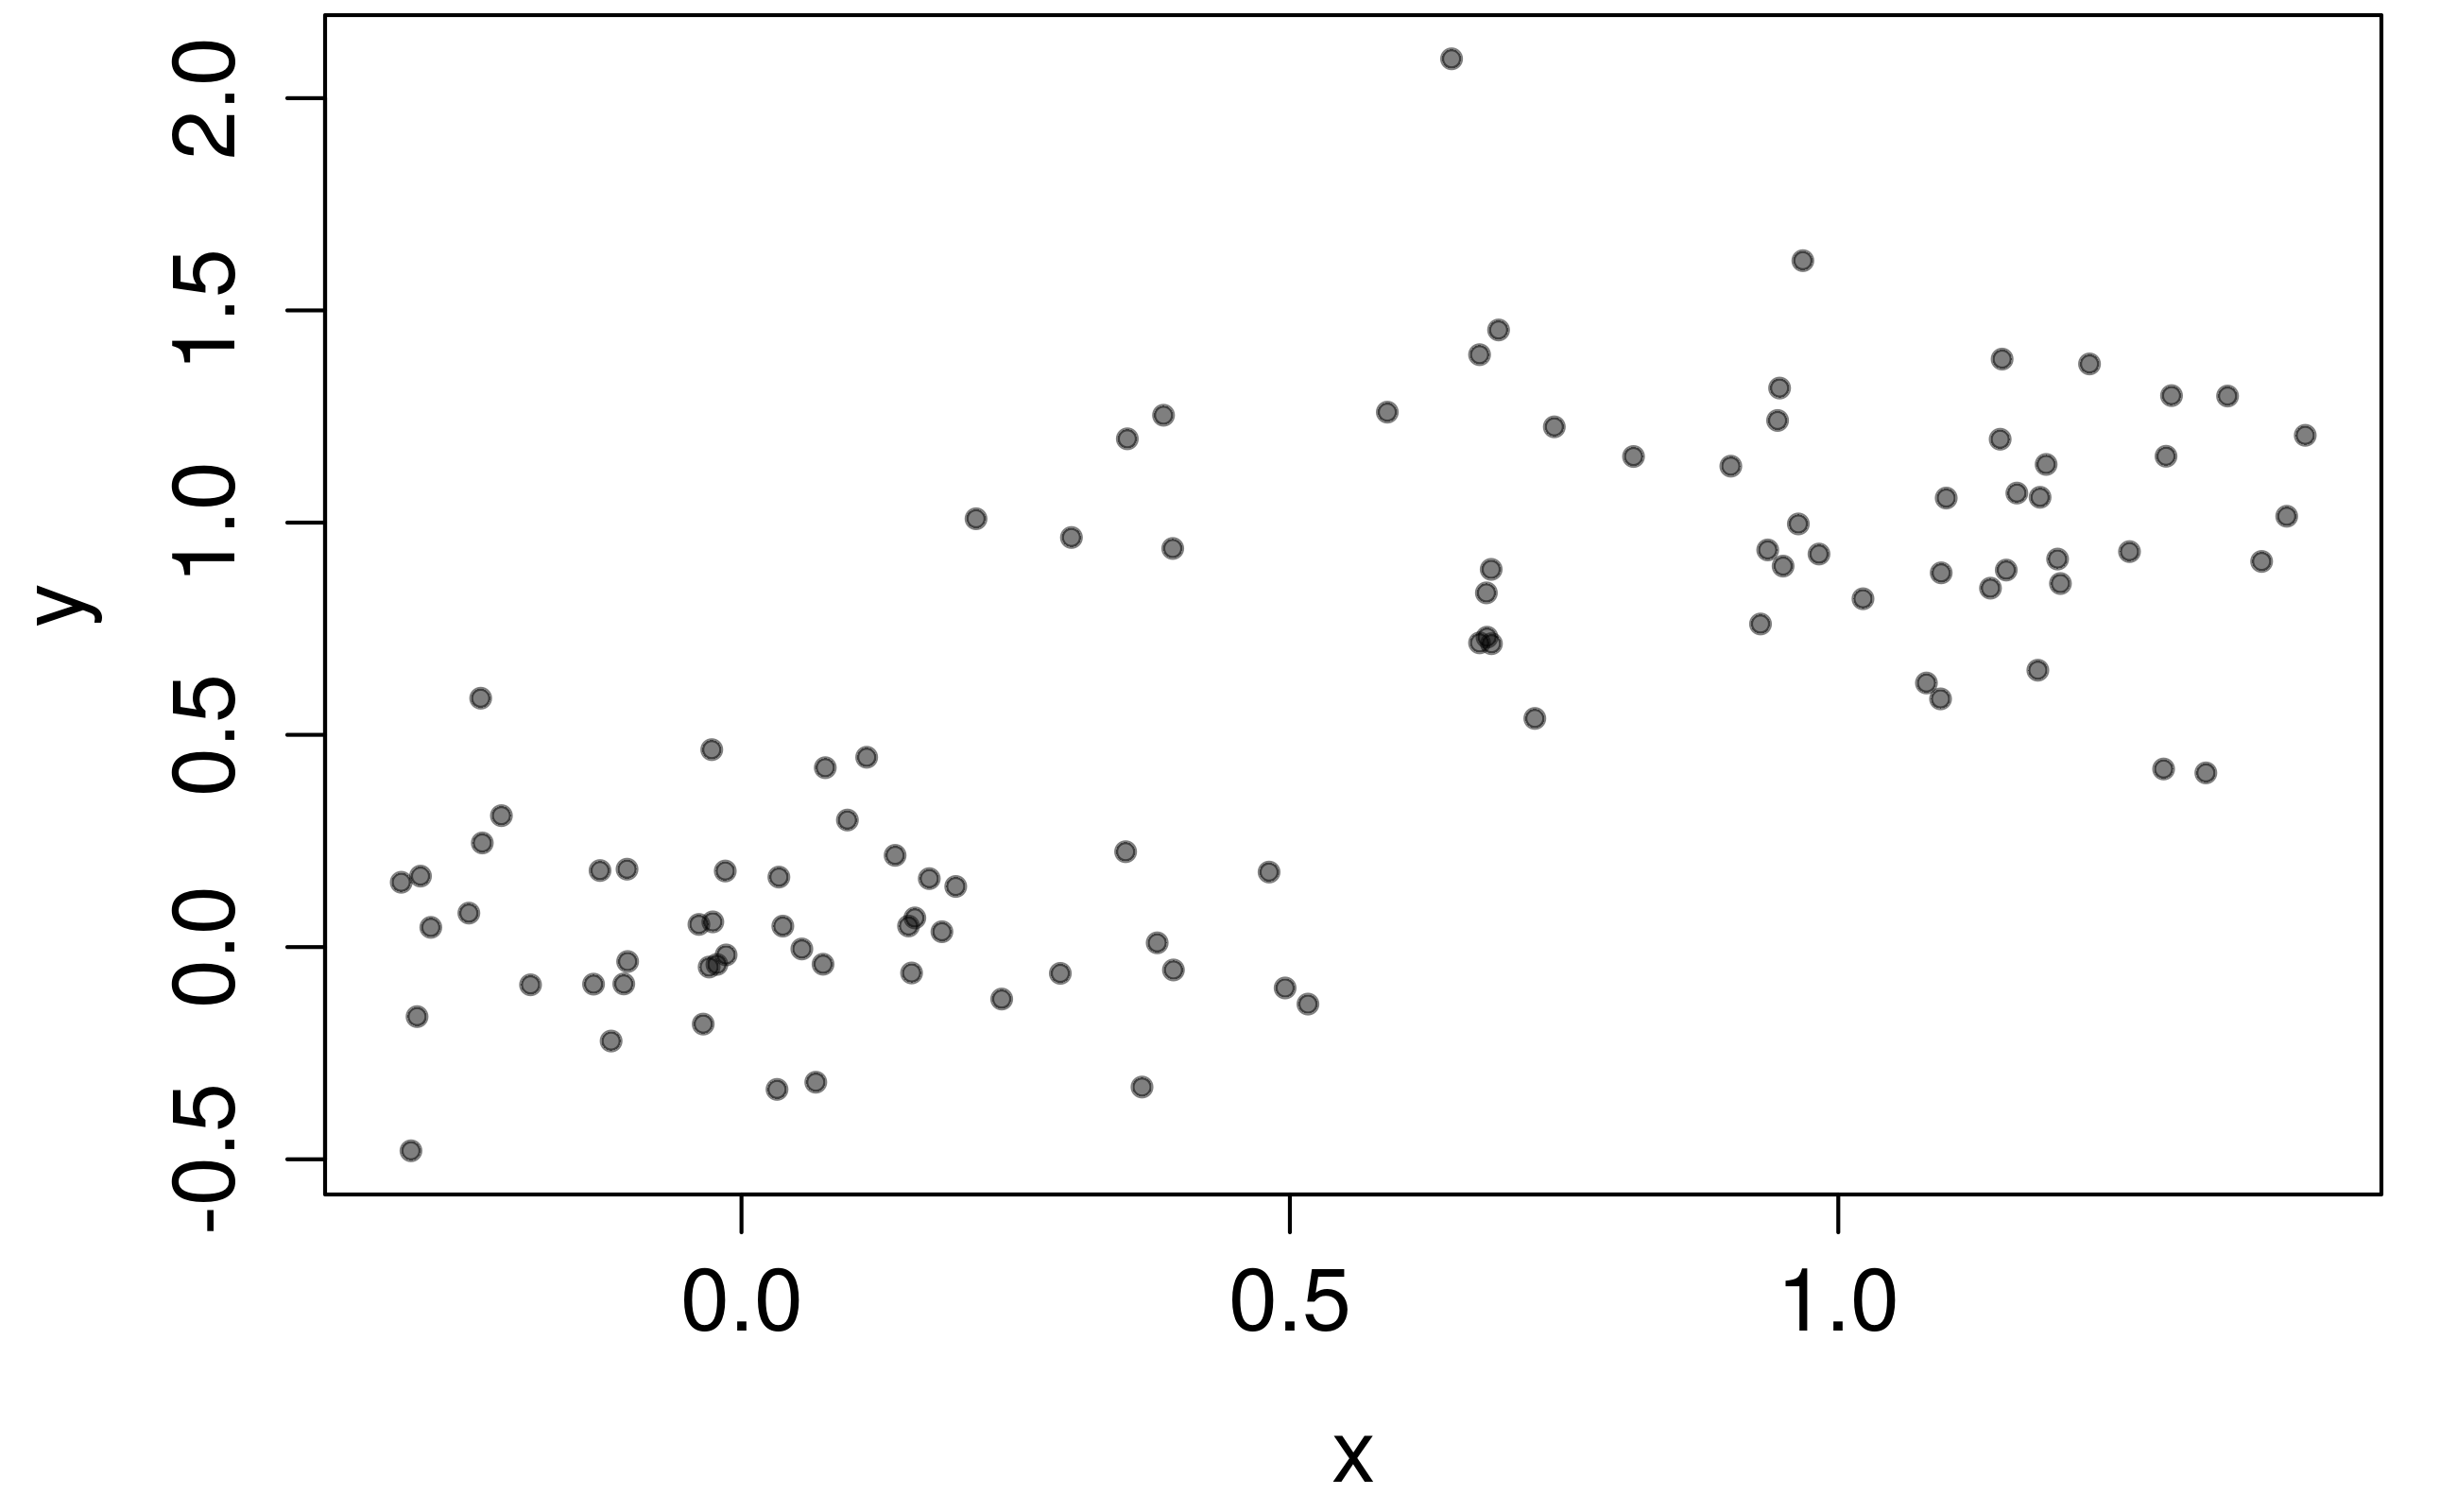
\includegraphics[width=.5\textwidth]{Bilder/test_clustering_points.png}
	}
	\hfill
	\subfloat{
		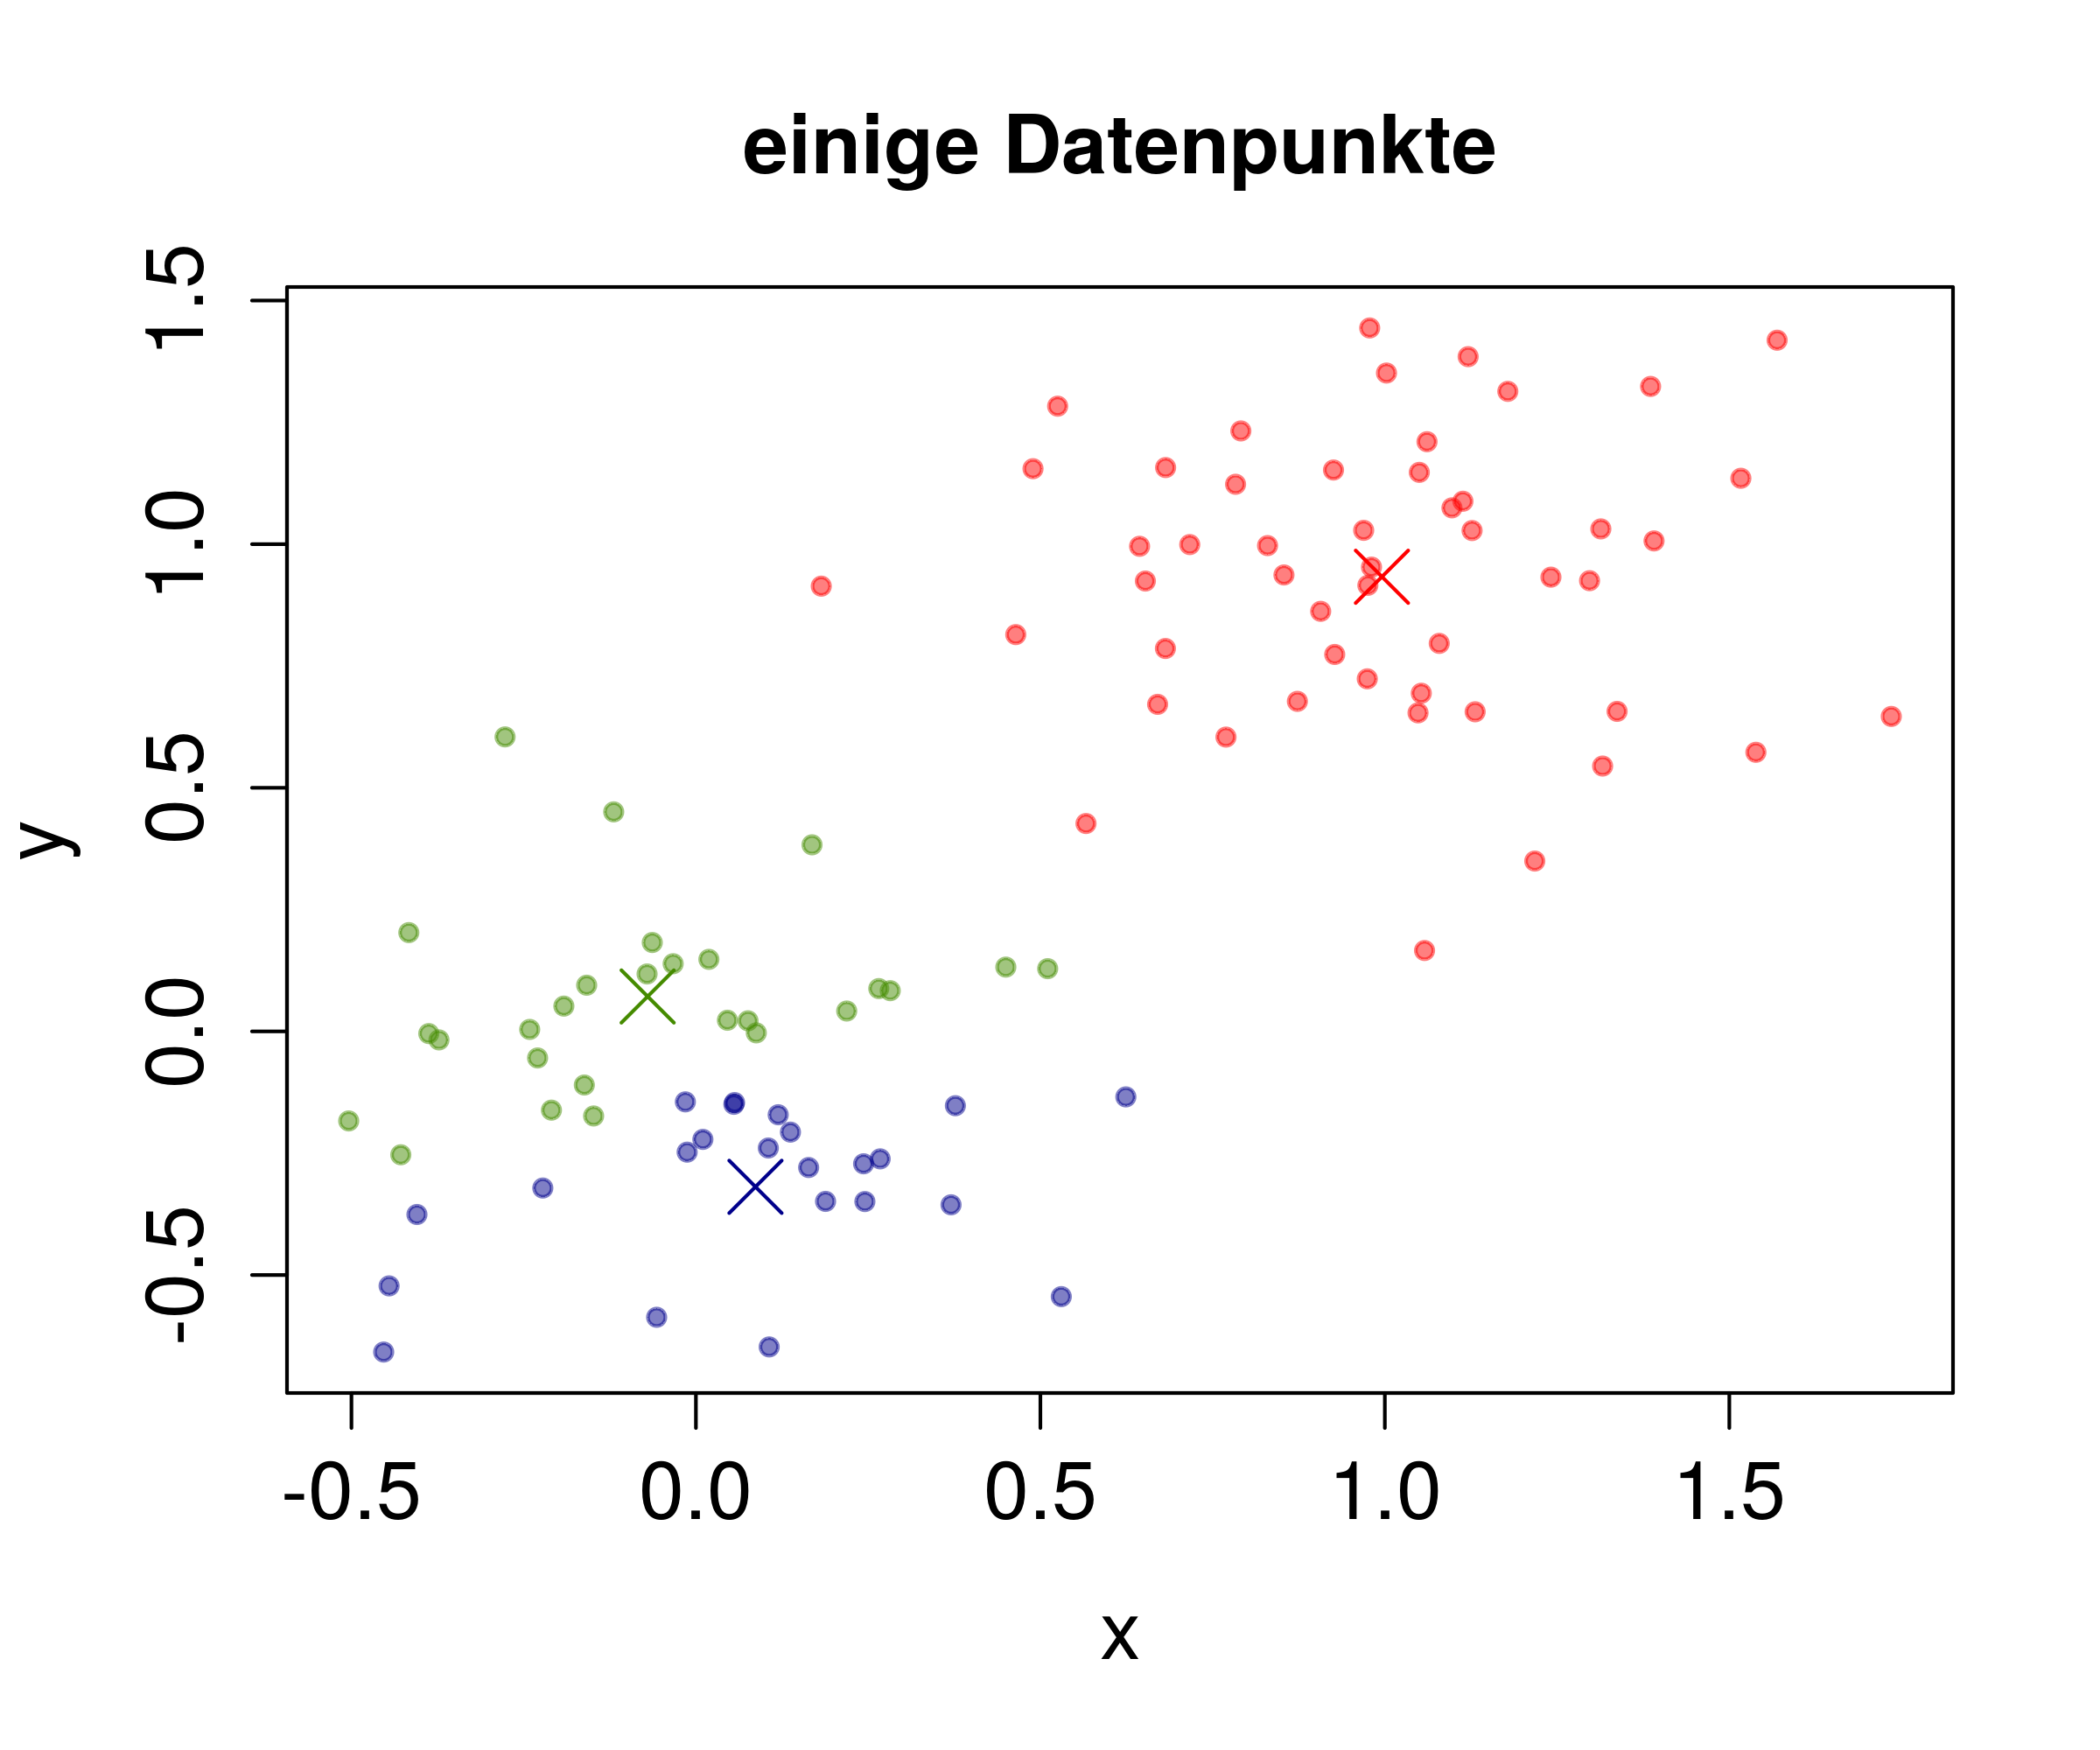
\includegraphics[width=.5\textwidth]{Bilder/test_clustering.png}
	}	
	\caption{Datenpunkte mit je einem Wert für x und y-Dimension. Rechts farbliche Markierung für die Zugehörigkeit zu drei vom k-Means-Algorithmus bestimmte Cluster. Ein Kreuz markiert den Mittelpunkt des Clusters (Mittelwert aller zugehörigen Punkte)}
	\label{fig:clustering_beispiel}
\end{figure} 

Ein einfacher Clustering-Algorithmus ist der k-Means-Algorithmus. Bei diesem muss zunächst die Anzahl Cluster $k$ festgelegt werden. Die $k$ Mittelwerte der Cluster mit zufälligen Werten initialisiert. Dann wird jeder Datenpunkt dem Cluster zugeordnet, dessen Mittelwert seinem am dichtesten ist. Danach werden die Mittelwerte der Cluster anhand der Ihnen zugeordneten Punkte berechnet und gesetzt. Das Neuzuordnen der Punkte und Berechnen der Mittelwerte wird nun solange wiederholt, bis sich keine Änderung der Zuordnung mehr ergibt. Als Endergebnis eines Cluster-Algorithmus erhält man eine Gruppierung der Datenpunkte in Mengen mit möglichst niedriger Varianz innerhalb eines Clusters und möglichst großer Varianz zwischen den Clustern.

%Die Aggregierung der Vorhersagen gesuchter Ausgabewerte von überwachten Lernalgorithmen ist eine recht simple Möglichkeit ein zuverlässigeres und exakteres Endergebnis zu erhalten. Verschiedene Modelle im Bereich des Ensemble Lernens verfolgen diesen Ansatz. Ein Ensemble ist dabei eine Menge von Vorhersage-Modellen. Nach Kantardzic \cite{kantardzic2011data} (Seite 236) kann ein solches Ensemble eine bessere Vorhersage treffen, als eines der in ihm enthaltenen einzelnen Modelle, wenn das Ensemble aus voneinander unabhängigen Modellen besteht, die mit einer Wahrscheinlichkeit größer als $0,5$ das richtige Ergebnis vorhersagen. Wobei er sich hier auf Klassifizierende Modelle bezieht, bei einem Regressionsmodell kann eine solche Wahrscheinlichkeit für die exakt richtige Ausgabe nicht erreicht werden, hier würde man eventuell von der Wahrscheinlichkeit sprechen, dass die Vorhersage in einem bestimmten Fehlerrahmen liegt. 
%An einem einfachen Beispiel verdeutlicht Kantardzic \cite{kantardzic2011data} (Seite 237) weshalb seine Behauptung gilt. Angenommen man hat $15$ voneinander unabhängige Modelle, jeweils mit einer Fehlerrate $\epsilon = 0,3$, das Ensemble bestehend aus diesen $15$ Modellen sagt die Klasse für einen Datenpunkt voraus, für die die Mehrheit der Modelle stimmt. Entsprechend liegt die Vorhersage des Ensembles falsch, wenn mehr als die Hälfte der Modelle eine falsche Vorhersage gemacht haben. Somit ergibt sich als Fehlerrate des Ensembles: 
%Der Fehler der einzelnen Modelle von $0,3$ konnte also um ein wesentliches Stück verkleinert werden.
%\begin{align*}
%	\epsilon _{ensemble}=\sum{15,i=8}{n\choose k}\epsilon^i(1-\epsilon)^(15-i) = 0,05
%\end{align*}
%\\
%\textbf{(generell , statt . bei Zahlen)}

\section{Künstliche Neuronale Netze}
\label{hintergrund_nn}
Bei künstlichen neuronalen Netzen, im Folgenden nur neuronale Netze genannt, handelt es sich um eine Methode aus dem Bereich des maschinellen Lernens zum Approximieren einer unbekannten Funktion, die der Relation zwischen zwei Datenmengen zugrunde liegt. Die Methode ist inspiriert von biologischen neuronalen Netzen, wie sie im Gehirn vorkommen. 
Sie verwenden einen statistischen Ansatz, ihre Lösung für das Problem wird zunächst zufällig im Lösungsraum angelegt und dann mit Hilfe eines Gradientenverfahrens optimiert.
Rojas \cite{Rojas:1996:NNS:235222} vergleicht neuronale Netze mit einer Black Box, also einem System mit beobachtbarer Ein- und Ausgabe, aber unbekannter innerer Verarbeitung der Informationen. 
Zur Verwendung eines neuronalen Netzes gibt man dem Netz eine Menge von Eingabevektoren $E \in \mathbb{R}^n$ mit jeweils zugehörigem Ausgabevektor $A \in \mathbb{R}^m$ vor und dieses versucht eine passende Funktion $F: \mathbb{R}^n \rightarrow \mathbb{R}^m$ zu finden. Dementsprechend handelt es sich hierbei um überwachtes Lernen, da eine gewünschte ideale Ausgabe vorgegeben wird.
Ein feedforward-Netz besteht aus einer Eingabeschicht, einer beliebigen Anzahl verborgener Schichten und einer Ausgabeschicht (siehe \ref{fig:Schichten}), wobei die Verbindungen aus jeder Schicht jeweils nur in die Nächsthöhere gehen. 
Die Eingabeschicht besteht meiner vorherigen Definition entsprechend aus $n$ Stellen, an denen die Werte eines Eingabevektors stehen. Jeder Eingabewert wird dann an jedes Neuron in der ersten verborgenen Schicht weitergegeben und dort verrechnet. Die Ergebnisse der Neuronen der verborgenen Schicht werden dann an die nächste Schicht gegeben und so weiter.
Die Ergebnisse der Ausgabeschicht bilden den Ausgabevektor mit Länge $m$.
Rekurrente Netze haben die gleiche Struktur, doch es können auch Verbindungen zu zurückliegenden Schichten vorkommen, dadurch ist die Berechnung zu einem Eingabevektor nicht mehr deterministisch bestimmt. Es müssen Berechnungs- und Determinierungsregeln festgelegt werden. 
\begin{figure}[h]
	\begin{center}
		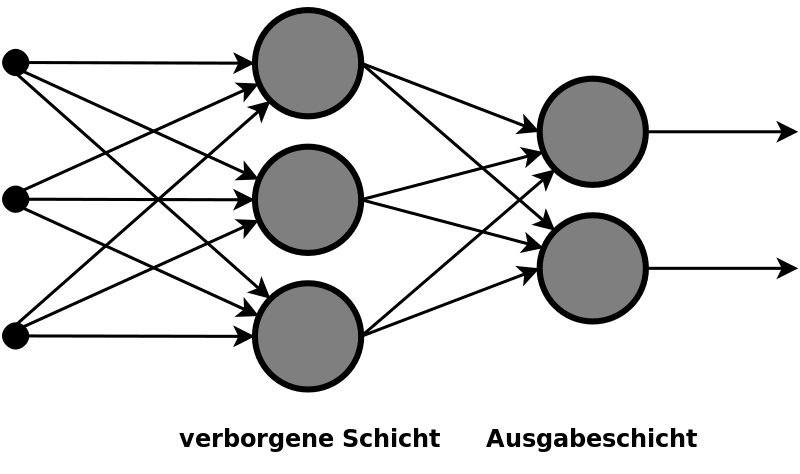
\includegraphics[totalheight=0.2\textheight]{Bilder/Multi-Layer_Neural_Network-Vector.png}
	\end{center}
	\caption{Zweischichtiges Netz (wiki)}
	\label{fig:Schichten}
\end{figure}
Jedes Neuron rechnet die eingehenden Eingabewerte mit einer zur Übertragungskante zugehörigen Gewichtung mit einer Übertragungsfunktion zusammen, die Anzahl der Eingaben ist hierbei unbegrenzt ("unlimited fan-in property" \cite{Rojas:1996:NNS:235222}). Die Übertragungsfunktion kann hierbei schlicht die Summe aller gewichteten Eingaben sein. Der errechnete Wert wird als Netzeingabe an die Aktivierungsfunktion gegeben. 
\begin{figure}[h]
	\begin{center}
		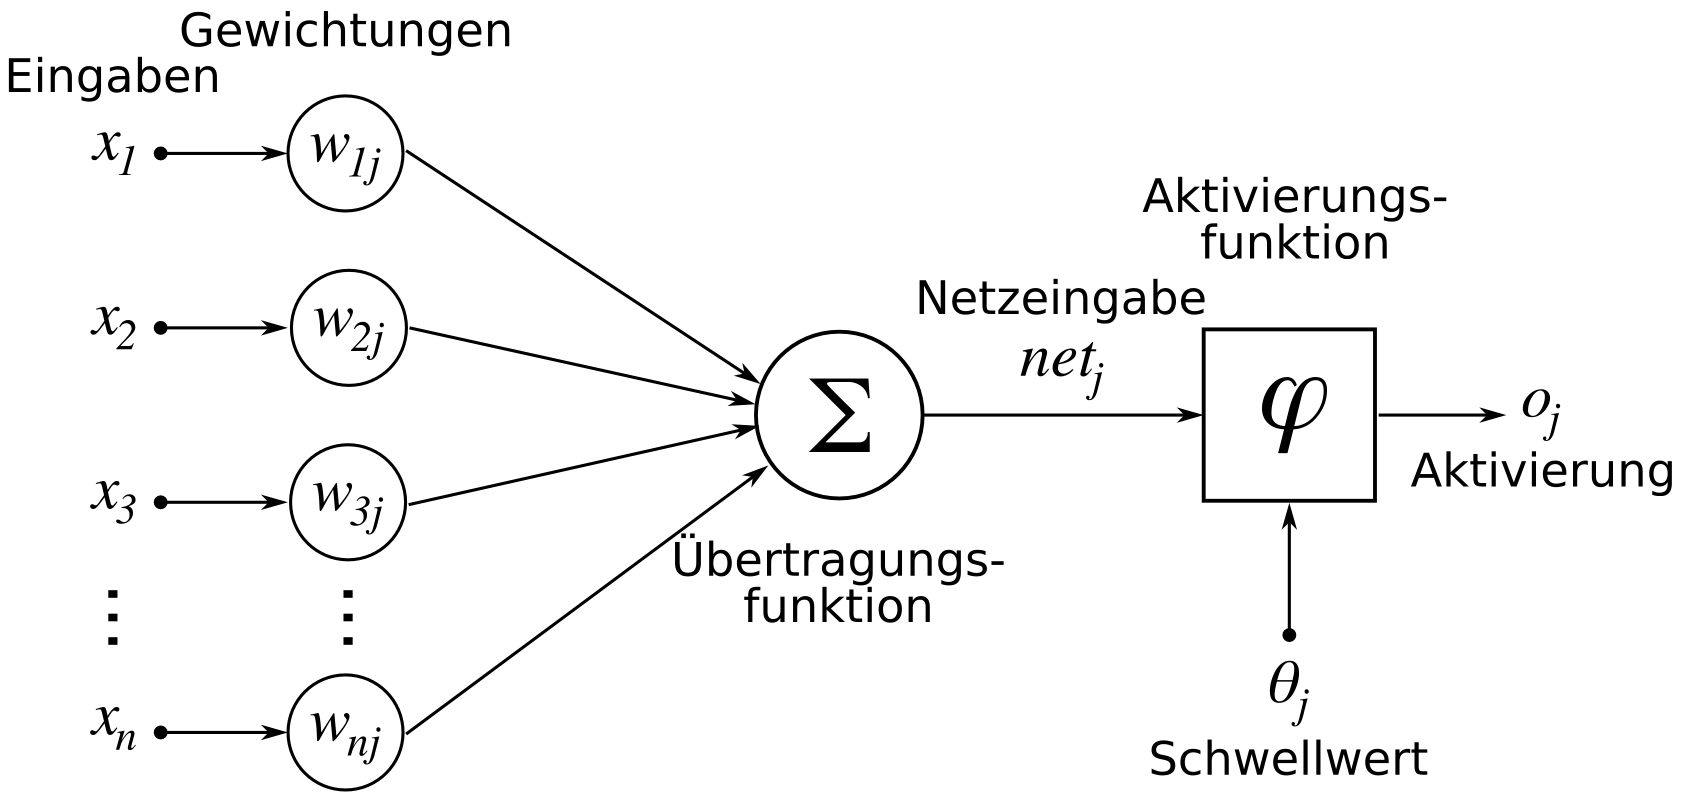
\includegraphics[totalheight=0.2\textheight]{Bilder/ArtificialNeuronModel_deutsch.png}
	\end{center}
	\caption{Schema eines künstlichen Neurons (wiki)}
	\label{fig:Neuron}
\end{figure}
Die Aktivierungsfunktion berechnet eventuell mit oder ohne einem Schwellwert die Aktivierung des Neurons, welche dann an alle verbundenen Neuronen der nächsten Schicht weitergegeben wird.
Die Aktivierungsfunktion kann beispielsweise eine simple Stufenfunktion sein, die allen Netzeingbaben kleiner des Schwellwertes eine Null und allen Eingaben größer gleich des Schwellwertes eine Eins zuweist.
Ein Neuron mit der gewichteten Summe aller Eingaben als Übertragungsfunktion und einer Stufenfunktion mit Schwellwert als Aktivierungsfunktion wird von Rojas \textit{Perzeptron} bezeichnet \cite{Rojas:1996:NNS:235222} (S. 60).
Ein feedforward-Netzwerk aus Perzeptrons, in dem jedes Neuron mit allen Neuronen der folgenden Schicht verbunden ist, wird als \textit{multilayer perceptron} (kurz MLP) bezeichnet.
Ein neuronales Netz lernt die Abbildung zwischen den vorgegebenen Paaren von Eingabe- und Ausgabedaten durch Anpassung der Gewichte an den Kanten, nachdem es mit zufällig initialisierten Kantengewichten gestartet ist.
Diese Anpassung geschieht beim MLP durch Fehlerrückführung (engl. backpropagation). Dabei wird der mittlere quadratische Fehler der berechneten Ausgabe gegenüber der vorgegebenen Ausgabe ermittelt und daraufhin unter Rücksichtnahme auf eine Lernrate mit Hilfe des Gradientenverfahren minimiert.

Vor der Anwendung von künstlichen neuronalen Netzen für ein Problem stellt sich die Frage, ob diese für das Problem geeignet sind. Dazu gibt es einige interessante mathematische Beweise.
Ein einzelnes Perzeptron kann alle linear separierbaren logischen Funktionen exakt approximieren \cite{Rojas:1996:NNS:235222} (S. 62-63). 
Wobei lineare Separierbarkeit definiert ist als:

Zwei Punktmengen A und B in einem n-dimensionalen Raum sind linear separierbar, wenn $n + 1$ reelle Zahlen $w_1,...,w_{n+1}$ existieren, sodass für jeden Punkt $(x_1,x_2,...,x_n) \in A$ die Ungleichung $\sum_{i=1}^{n} w_ix_i \ge w_{n+1}$ gilt und für jeden Punkt $(x_1,x_2,...,x_n) \in B$ $\sum_{i=1}^{n} w_ix_i < w_{n+1}$ \cite{Rojas:1996:NNS:235222} (S. 63)

\begin{figure}[h]
	\begin{center}
		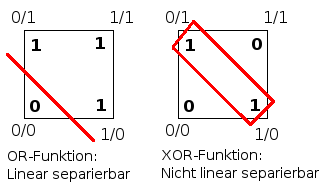
\includegraphics[totalheight=0.2\textheight]{Bilder/Lineare_Separierbarkeit.png}
	\end{center}
	\caption{Lineare Separierbarkeit von Funktionen (wiki)}
	\label{fig:Separierbarkeit}
\end{figure} 

Diese Beschränkung gilt allerdings nicht für ein Netzwerk von Neuronen. Bereits ein zweilagiges Netzwerk aus noch simpleren McCulloch-Pitts-Zellen kann jede beliebige logische Funktion berechnen \cite{Rojas:1996:NNS:235222} (Seite 37).
Für MLPs hat Cybenko \cite{cybenko:mcss} bewiesen, dass sie beliebige kontinuierliche Funktionen auf einer kompakten Teilmenge des euklidischen Raums $\mathbb{R}^n$ approximieren kann. Der entsprechende Satz hierzu ist das \textit{universal approximation theorem}.

\bigskip
\paragraph{Zusammenfassung:}
\textit{ 
	Das Kapitel hat einen kurzen Abriss der für diese Thesis relevanten Themen geliefert. Es wurde festgestellt, dass die Vorhersage von E/A-Laufzeiten im Hochleistungsrechnen eine komplexe Aufgabe ist. Zusätzlich zu dem ohnehin aufwendigen E/A-System eines normalen Rechners müssen die Komplilkationen durch die Vernetzung des Hochleistungsrechners in Betracht gezogen werden.
	Solange die E/A-Leistung durch eine kontinuierliche Funktion beschrieben werden kann und alle dafür benötigten Informationen zur Verfügung stehen, kann ein künstliches neuronales Netz das Problem lösen.
}


\chapter{Verwandte Arbeiten}
\textit{%
	Es finden sich keine wissenschaftlichen Veröffentlichungen die sich auch mit dem Einsatz von neuronalen Netzen zur Vorhersage von E/A-Leistung im Hochleisungsrechnen befassen. Jedoch werden die verschiedenen Teilgebiete des Themas behandelt. Als Erstes gehe ich auf einige Arbeiten ein, die allgemeine E/A-Leistungsvorhersage behandeln, um dabei weniger Umschreiben zu müssen führe ich zunächst zwei Kategorien von Lösungsansätzen ein. Danach gehe ich kurz auf die Verwendung von neuronalen Netzen zur Leistungsvorhersage und die Leistungsmodellierung im Hochleistungsrehcnen ein.
}
\bigskip

\section{Leistungsvorhersage von Ein-/Ausgabe}

\subsection{Kategorisierung}
Das Problem, die Zugriffszeiten auf Festplatten vorherzusagen, kann im wesentlichen durch zwei verschiedene Ansätze gelöst werden \cite{Crume:2013:FML:2538542.2538561} (S. 1). Zum einen kann man versuchen das Festplattensystem in einem Modell nachzubilden, indem Hardwaredetails, wie die Rotationsgeschwindigkeit der Platte, die Reaktionszeit und Geschwindkeit des Lesekopfs, sowie das Zusammenspiel der Komponenten bekannt sind oder entsprechende Parameter durch gezielte Untersuchung approximiert werden. Mit diesem möglichst exakten Modell können dann Zugriffe simuliert und die Laufzeit des Modells gemessen werden. Diese Messung kann daraufhin als Vorhersage für das reale System verwendet werden.
Der zweite Ansatz ist auch der in dieser Arbeit evaluierte, es wird von dem eigentlichen Festplattensystem abstrahiert und stattdessen ein mathematisches Modell gesucht, das das Verhalten des Systems möglichst genau beschreibt.
Zur Entwicklung des mathematischen Modells werden gemessene Leistungswerte von Festplattenzugriffen untersucht, um daraus passende Parameter für das Modell abzuleiten.
Ich unterscheide daher im Folgenden zwischen dem Modellierungssansatz, bei dem versucht wird das Festplattensystem nachzubilden (in der englischen Fachliteratur auch als \textit{analytic device modeling} und \textit{simulation modeling} bzw. allgemeiner als white-box modeling bezeichnet) und dem Interpolationsansatz, bei dem ein numerisches Modell entwickelt wird. Da man hier ohne Wissen über die inneren Zustände des Systems modelliert, wird dieser Ansatz auch als \textit{black-box modeling} bezeichnet. 

\subsection{Modellierungssansatz gegenüber Regressionsansatz}
Die Nachteile von Modellen mit Modellierungssansatz liegen insbesondere darin, dass sie aufwendig zu konfigurieren sind \glqq In fact, one of us (Oldfield) spent several months configuring DiskSim to model an existing device\grqq{} \cite{Crume:2013:FML:2538542.2538561} (S.1) und naturgemäß schnell veraltern, da sie jeweils an spezielle Hardware angepasst sind. Der Vorteil dagegen ist, dass sie bei korrekter Konfiguration sehr präzise sind, wie z.B. hier gezeigt \cite{Ruemmler94anintroduction}.

Der Interpolationsansatz ist in der Anwendung einfacher und flexibler, da es sich automatisch an das System anpasst. Dafür erwartet man aufgrund der fehlenden analytischen Einsicht ins System ungenauere Prognosen. Für die Anwendung im HPC-Bereich spielt der analytische Ansatz eine untergeordnete Rolle, da hier unterschiedliche Festplattensysteme zusammenarbeiten und stark mit der Netzwerkarchitektur verstrickt sind, sodass eine entsprechende Analyse des Systems zu aufwendig wird. \glqq Furthermore, [...] building an accurate model or simulator using white box method cannot be a genereal solution in serving a variety of very different workloads\grqq{} \cite{DBLP:conf/npc/ZhangLZJC10} (S.2, Zeile 20-24).

Eine weitere Arbeit, in der ein Modellierungsansatz genutzt wird stammt von Lebrecht et al. \cite{Lebrecht:2009:10.1109/QEST.2009.31}. Darin wird besonders auf ein Verfahren eingegangen, das dafür sogt, dass E/A-Anfragen in einer Reihenfolge abgearbeitet werden, die die notwendigen Bewegungen des Lese-/Schreibkopf möglichst gering hält.

Bei Arbeiten, in denen ein Interpolationsansatz genutzt wird, werden verschiedene Data-Mining bzw. stochastischen Methoden angewandt, beispielsweise eine Kombination aus Regressionsbäumen und Stützvektormaschinen \cite{Dai:2012:SDP:2477169.2477214} oder Bagging Klassifikation und Regressionsbäumen \cite{DBLP:conf/npc/ZhangLZJC10}. Verschiedene statistische Methoden werden von Kelly et al. untersucht \cite{Kelly04inducingmodels}.
Ein in diesem Kontext beachtenswertes Patent \cite{gough2012predicting} zeigt ein Anwendungsbeispiel für E/A-Leistungsvorhersage mit Regressionsansatz. Dabei wird mit Hilfe maschinellen Lernens ein Überwachungssystem für Festplatten entwickelt, das einen Ausfall des Systems anhand der beobachteten internen Zustände vorhersagt. 

\section{Leistungsvorhersage mit neuronalen Netzen}

Wie bereits im Kapitel \ref{hintergrund_nn} beschrieben wurde, gibt es einige Forschung zu der Frage der Mächtigkeit von neuronalen Netzen. \cite{Rojas:1996:NNS:235222} und \cite{cybenko:mcss} behandeln die Modellierung von nicht-linearen Systemen. Darüber hinaus \cite{suykens2012artificial} hat \textit{universal approximation theorem} für neuronale Netze bewiesen. Es ist nicht bekannt, welche Komplexität für die exakte Beschreibung eines Hochleistungs-E/A-System benötigt wird. Der Mächtigkeit von neuronalen Netzen sollte allerdings zumindest zur Bestimmung einer Näherung mit Berücksichtigung der wesentlichen Einflüsse ausreichen.

Ein mathematisch anspruchsvolles Verfahren mit Interpolationsansatz unter der Verwendung von neuronalen Netzen wurde von Adam Crume et al. \cite{Crume:2013:FML:2538542.2538561} entwickelt. Sie gehen davon aus, dass der entscheidende Faktor bei der Vorhersage von Zugriffszeiten in der Erkennung von periodischen Mustern liegt. Diese Annahme ist für eine einzelne Festplatte gerechtfertigt, da man die Zugriffszeit grob in zwei Teile aufteilen kann, zum einen die Bewegung des Lesekopfs auf die richtige Spur und die Bewegung des Kopfes entlang der Spur zum richtigen Punkt, auch wenn diese beiden Bewegungen in der Realität überlappen. Jede Festplattenspur hat entsprechend des Radius eine andere Periodendauer.
Durch eine Fourier-Analyse finden sie die Hauptfrequenzen heraus und können diese dann nutzen, um mit einem neuronalen Netz Vorhersagen zu treffen.
Eine Schwierigkeit in dieser Arbeit ist unter anderem, dass durch die große Anzahl Perioden nur ein kleiner Ausschnitt der Festplatte in seiner Gesamtheit, also alle möglichen Paare von Ausgangs- und Endspuren, untersucht werden kann.

In einer weiteren Arbeit führen Crume und Maltzahn diesen Ansatz fort \cite{crumeadammaltzahncarlos2015}. Sie zeigen, dass die Periodizität der Festplattenlatenzen auch ohne Fourier-Analyse von neuronalen Netzen ausgenutzt werden kann. Dazu geben sie den verwendeten Netzen zusätzliche Sinuskurven als Eingabeattribute.

Der hohe Aufwand für das Auffinden interessanter Frequenzen in einer einzelnen Festplatte zeigt, dass dieser Ansatz für das komplexe E/A-System im Hochleistungsrechner zunächst einmal nicht geeignet erscheint.

\section{Leistungsvorhersage im Hochleistungsrechnen}

Im Hochleistungsrechnen ist die Leistungsanalyse eine wichtige Aufgabe. Mit dessen Hilfe können Aussagen darüber gemacht werden, wie effizient die Hardware ausgenutzt wird und Optimierungen vorgeschlagen werden. 

So simulieren Liu et. al \cite{liu2011towards} beispielsweise den Scheduling-Algorithmus vom Dateisystem. Dazu verwenden sie DiskSim \cite{Bucy08thedisksim} zur Vorhersage von Festplattenzugriffszeiten.

Interessant ist die Arbeit von Molina-Estolano, Maltzahn, Bent und Brandt in der sie ein Simulationsprogramm für parallele Dateisysteme vorstellen \cite{molina2009building}. Sie ermöglichen es auf einem vergleichsweise kleinen Rechner, dass Dateisystem eines Hochleistungsrechners abzubilden. Mit dieser Simulation kann mit wenig Aufwand ein großes Dateisystem analysiert werden, um die Ergebnisse anschließend am richtigen System umzusetzen. Das verwendete Modell ist dabei naturgemäß eine Abstraktion des richtigen E/A-Systems und eignet sich daher nicht dafür das Leistungsverhalten im Detail zu untersuchen.

Eine Arbeit aus dem Hochleistungsrechnen, die sich mit Vorhersage von E/A-Leistung befasst ist die von Kunkel et. al \cite{UMLTPTPONI15}. Hier wird versucht mit Hilfe von Entscheidungsbäumen die performantesten Parameter für nicht zusammenhängende Zugriffe auf Dateien durch ROMIO, einer Implementierung von MPI-2 I/O, zu finden.
Dabei sagen sie mit Entscheidungsbäumen die Leistung für verschiedene Parameter auf den Daten voraus. Dies geht schneller, als die Parameter in der Anwendung zu testen. Anhand der Vorhersagen können dann die besten Parameter gewählt werden. (\textbf{habe ich das richtig verstanden}?) 
Entscheidungsbäume können keine sehr komplexen Probleme lösen, sie können nur Entscheidungen als eine Aneinanderreihung von linearen Separationen des Werteraums treffen. Dennoch sind die mit dieser Methode erzielten Ergebnisse zufriedenstellend. Dies lässt vermuten, dass mit Hilfe von komplexeren Methoden des maschinellen Lernens, wie neuronalen Netzen noch bessere Ergebnisse erzielt werden könnten.
Hier findet sich ein potenzielles Anwendungsgebiet der Ergebnisse dieser Bachelorarbeit.

\paragraph{Zusammenfassung:}
\textit{
	Nach der Betrachtung verwandter Arbeiten kann resümiert werden, dass E/A-Leistungsvorhersage mit neuronalen Netzen kein neuer Ansatz ist und bereits einige Erfolge erreicht hat. Die Übertragung der Konzepte im Detail scheint dagegen aufgrund der Analyse eines komplexen E/A-Systems eines Hochleistungsrechners schwierig zu sein.
}

\chapter{Gestaltung der Analyse}
\textit{
In diesem Kapitel wird darauf eingegangen, wie die Ziele dieser Arbeit erreicht werden sollen und welche Ansätze dabei verfolgt werden.
Zunächst wird dargestellt, welche die Modellvorstellung des untersuchten Systems 	den weiteren Untersuchtungen zugrunde liegt.
Dann gehe ich auf die beiden verwendeten Methoden der Leistungsvorhersage ein, zum einen die direkte Vorhersage von Leistung als E/A-Laufzeiten, zum anderen die Vorhersage von Ausreißern über Laufzeitbereiche. 
Daraufhin wird das Kernstück dieser Arbeit behandelt. Die unterschiedlichen untersuchten Modelle. Die Modelle werden in Klassen unterteilt. Die Analyse der verschiedenen Klassen geschieht zu unterschiedlichen Zwecken und sollen in einer bestimmten Weise Einsicht über das komplexe E/A-System eines Hochleistungsrechners geben. Als letztes werden die verwendeten Modelle im Detail gezeigt und auf deren Anwendung eingegangen.
}
\bigskip

\section{Modell der Ein-/Ausgabe}
\label{ea_modell}
Um eine Idee dafür zu bekommen, wie die Modelle in etwa gestaltet sein müssen, um die Zugriffszeiten abbilden zu können, wird hier zunächst ein grobes Modell der E/A aufgestellt.

Anhand der Verarbeitung eines Leseaufrufs gehe ich die Stufen des E/A-Systems durch. Wie in \ref{E/A} beschrieben hängt die Zugriffszeit davon ab, in welcher Speicherebene sich die angefragten Daten befinden.
Für die Zugriffszeit kann im wesentlichen unterschieden werden, ob sich die angefragten Daten bereits innerhalb des anfragenden Rechnerknoten befinden oder diese von einer Festplatte außerhalb des Knotens geholt werden müssen.
Falls die Daten sich nicht im Speicher des Rechnerknotens befinden, muss als erstes eine Anfrage an das angebundene E/A-System gestellt werden.
Dort ist der reine Verwaltungsaufwand der Anfrage im wesentlichen für alle Aufrufe konstant sein, denn sie sieht strukturell für aufwendige Aufrufe nicht anders aus, als für weniger aufwendige.
Daraufhin muss das E/A-System die Festplatten ansprechen (evt. auch mehrere) auf der die relevante Datei liegt. Der Aufwand für den Aufbau der Verbindung zum Speicherort der Datei ist dabei von der Struktur des Netzwerkes abhängig. Die Festplatte liest die Daten aus und schickt sie über das Netzwerk an den Rechnerknoten auf dem sie benötigt werden.
Nun müssen die angefragen Daten aus dem Arbeitsspeicher des Knotens über die Cache-Ebenen in den Prozessor geladen werden. 
Falls die Daten bereits im Arbeitsspeicher oder einem der Caches liegen, werden entsprechend weniger Schritte durchgeführt.
Für einen Schreibzugriff gilt im Wesentlichen ein ähnlicher Ablauf, der Datenfluss ist nur umgekehrt.

Es können drei voneinander unabhängige Anteile der Zugriffszeit unterschieden werden. Die Zeit, die für die Verwaltung der E/A-Anfrage und die Dateiübertragung über das Netzwerk benötigt wird (tNetzwerk), sowie für die Verarbeitung auf der Festplatte (tHDD) und für das Lesen/Schreiben von dem Arbeitsspeicher und der Caches (tMem).

In allen Bereichen gibt es jeweils einen konstanten Anteil und einen Anteil, der von der aufgerufenen Datei abhängt. 
Der Anteil der Zugriffszeit, die für jeden Aufruf konstant ist, ist für die Modellierung weniger spannend und sollte bereits durch einfache linerare Modelle darstellbar sein, dieser Teil wird im Folgenden nicht weiter berücksichtigt.

Der Netzwerkabhängige Teil ist zum einen vom genauen Speicherort der aufgerufenen Datei, sowie der Größe der Datei abhängig. Der Datenfluss über das Netzwerk hängt von dessem Durchsatz ab, dieser sollte nach kurzer Verbindungsaufbauphase konstant sein. Im Rahmen meiner Instrumentierungsmöglichkeiten ist es nicht möglich die Abhängigkeit der Zugriffszeit von Speicherort im Netzwerk direkt vorherzusagen. Dazu wäre ein Einblick in eine Datenbank notwendig, aus der sich solche Informationen ableiten ließen, oder eine solche Wissensbasis müsste selbst aufgebaut werden.
tMem ist am einfachsten zu modellieren, denn der hier auftretende Direktzugriffsspeicher (engl. Random-Access Memory) kennzeichnet sich gerade dadurch, dass der Zugriff auf alle Datenblöcke mit geichem Aufwand verbunden ist.
Ansonsten hängt die Zugriffszeit vom Durchsatz des Speichers ab.
Eigentlich handelt es sich bei tMem um die Zusammensetzung der Zeitanteile von Arbeitsspeicher und der Caches, es wird im Modell jedoch vom langsamsten Speicher dominiert, der angesprochen werden muss. Die höheren Ebenen der Zwischenspeicher bleiben jeweils unbeachtet.
Die Festplatte ist ähnlich Komplex wie das Netzwerk. Wie beim Netzwerk ist die Zugriffszeit zum einen von dem genauen Speicherort der angefragten Datenblöcke und zum anderen vom Durchsatz der Festplatte abhängig.
Die Abhängigkeit von der Speicherposition schlägt sich in dem Abstand des Aufenthaltsortes des Lesekopfes vor dem Aufruf zu dem Zielort auf der Festplatte nieder. Die zu überwindende Strecke des Lesekopfes hängt dabei grob von dem Abstand der zuletzt zugegriffenen Speicherposition zur nächsten gesuchten Speicherposition ab. Dieser Abstand im Folgenden wird dieser Abstand als Delta-Abstand bezeichnet.
Der zeitliche Aufwand zum Überwinden des Delta-Abstandes ist von Hardwarecharakteristika der Festplatte abhängig. Zum einen die Zeit, die der Lesekopf benötigt, um von der aktuellen Festplatten-Spur zur Zielspur zu kommen und zum anderen, die Rotationszeit der Magnetscheibe, die den Lesekopf in der Horizontalen zur richtigen Stelle befördert. 
Dieser Spurwechsel und die Rotation geschehen dabei gleichzeitig. Ansonsten ist die Zugriffszeit linear von dem Durchsatz der Festplatte und der Größe des angefragen Abschnittes abhängig.

tMem müsste nach diesem Modell vollständig durch ein lineares Modell dargstellt werden können. Dagegen ist dies für tNetzwerk und tHDD nur bedingt der Fall.
Netzwerk und Festplatte haben einen je nach Zugriffsgröße dominierenden linearen Anteil, jedoch auch einen Speicherort abhängigen.
Die Durchsätze von tMem, sowie tHDD sind Hardware bedingt von der Art des Zugriffs abhängig, es muss also zwischen Lese- und Schreibzugriffen unterschieden werden, dies ist geschieht im Folgenden über den Operationstyp (OpTyp).
Das Modell für die Ein-/Ausgabe in dieser Arbeit entspricht letztendlich

\begin{align*}
tGesamt &= tHDD + tNetzwerk + tMem\\
\text{mit}\\
tHDD &= \frac{Zugriffsgrö\text{ß}e}{Festplattendurchsatz(OpTyp)} + Festplattenlatenz(Delta\text{-}Abstand) \\
tNetzwerk &= \frac{Zugriffsgrö\text{ß}e}{Netzwerkdurchsatz} + Netzwerklatenz(Netzwerkspeicherort) \\
tMem &= \frac{Zugriffsgrö\text{ß}e}{Speicherdurchsatz(OpTyp)} + Speicherlatenz
\end{align*}

Latenz bezeichnet die Verzögerungszeit, bis die Datenübertragung angelaufen ist.
Die Vermutung in dieser Arbeit ist, dass sich E/A-Aufrufe in verschiedene Pfade unterteilen lassen, dabei entspricht der Pfad der Verbindung vom aufrufenden Prozess zur aufgerufenen Datei. Die Zugriffszeit eines solchen Pfades wird von der langsamsten Komponente auf dem Weg dominiert. 
Ein perfektes Modell könnte unter Kenntnis dieses Pfades und der Dateiattribute die Dauer des Zugriffs exakt vorhersagen.

Relevante und Messbare Größen sind nach diesem Modell die Größe des gelesenen/geschriebenen Bereichs, der Operationstyp und der Delta-Abstand. 
Das Tripel $(Zugriffsgrö\text{ß}e,OpTyp,Delta\text{-}Abstand)$ bezeichne ich als Attribut-Set, es charakterisiert einen E/A-Aufruf. Alle Messungen zu Speicheraufrufen mit dem selben Attribut-Set hätten nach diesem Modell idealerweise die selbe Laufzeit. 

\section{Leistungs- und Ausreißervorhersage}
Mit den im Weiteren entwickelten Modellen soll untersucht werden, wie gut es gelingt den Aufwand der E/A-Aufrufe vorherzusagen. 
Für die Berechnung eines Modells werden jeweils Informationen über das zu beschreibende System benötigt. Dies wird durch die Vermessung E/A-Aufrufen geschehen.
Die Vermessung wird als Benchmark-Test bezeichnet und wird in der Evaluation entwickelt. 
Wenn Messdaten vorliegen, kann das Modell einen Teil der Daten als Trainingsdatensatz zum Lernen nutzen, die restlichen Daten sind dem Modell unbekannt und bilden den Testdatensatz. Die Vorhersagen der Modelle zum Testdatensatz können dann mit den tatsächlichen Werten verglichen werden. Dies ist die Leistungsvorhersage vom Modell zum System. 
Desweiteren wird die Ausreißervorhersage des Modells betrachtet werden. Als Ausreißer werden dabei die Messungen bezeichnet, die eine ungewöhnlich schnelle oder langsame Laufzeit haben. In unseren Messdaten werden die langsamsten und die schnellsten $10\%$ der Messungen jedes Attribut-Sets als Ausreißer bezeichnet. Es handelt sich hierbei in diesem Kontext nicht um invalide Messungen, für die die Instrumentierung des Experiments verantwortlich ist. Stattdessen kann es beispielsweiese sein, dass das System punktuell sehr ausgelastet war. 
Bei der Ausreißervorhersage wird geprüft, ob das Modell korrekt voraussagen kann, dass die Laufzeit einer E/A-Anfrage zu den Ausreißern gehört. Da es sich bei den Ausreißern nicht um Messfehler handelt ist eine solche Vorhersage prinzipiell möglich, erfordert allerdings eine sehr gute Einsicht ins System.
Man könnte die Ausreißervorhersage auch als Test auf den schwierigsten Daten ansehen. 
Es würde für die Qualität eines Modells sprechen, wenn es sowohl eine gute Leistungsvorhersage, auch eine gute Ausreißervorhersage macht. Da die Informationen, die den Modellen zur Verfügung stehen allerdings nicht für eine verlässliche Ausreißervorhersage ausreichen sollten (beispielsweise wäre dazu Wissen über parallel laufende Prozesse von anderen Benutzern des Hochleistungsrechners notwendig), könnte dieser Test auch ein Maß für eine zu starke Adaption an die Trainingsdaten sein.

\section{Modellklassen}
Modelle unterscheiden sich an den Informationen, die Ihnen über die Messdaten zur Verfügung stehen.
Da es sich bei der E/A-Leistungsvorhersage um ein komplexes Problem handelt, steht nicht a priori fest, wie eine passende Modellierung auszusehen hat. 
In dieser Arbeit wurden daher verschiedene Ansätze getestet.

Um besser zu verstehen, welche Ideen einem Modell zugrunde liegen und zur einfacheren Beschreibung der Modelle führe ich verschiedene Kategorien von Modellen ein, die jeweils einem bestimmten Ansatz entsprechen.
Die Modellklassen unterscheiden sich in ihrer Herangehensweise ans Problem. Modelle, die den selben Klassen zugehören, unterscheiden sich an den Informationen, die ihnen über die Messdaten zur Verfügung stehen.

\subsection{Triviale und höhere Modelle}
Triviale Modelle werden auf einfache Weise mit klassischen mathematischen Methoden mit relativ geringem Rechenaufwand berechnet.
Die höheren Modelle in dieser Arbeit basieren dagegen auf neuronalen Netzen und müssen aufwendig trainiert werden.

Die trivialen Modelle sind zum einen beim Erkunden verschiedener Ansätze hilfreich, zum anderen dienen sie dem Vergleich zu den aufwendigeren Modelle und stellen eine untere Schranke für deren Leistungen dar.
So kann an den Ergebnissen eines Modells, das bloß lineare Zusammenhänge beschreiben kann, untersucht werden, ob die Daten in linearer Weise beschrieben werden können. Die Erwartung ist, dass die höheren Modelle wesentlich bessere Ergebnisse zeigen, als die trivialen. Wenn dies nicht der Fall ist, war entweder die Modellierung schlecht oder die verwendeten Informationen über die Messdaten waren unzureichend für eine zufriedenstellende Beschreibung.
Eine Ausnahme bilden dabei \textit{unfaire} triviale Modelle, die mit Informationen ausgestattet sind, die sie als legitimes Modell nicht haben dürften. Unfairen Modellen standen sämtliche Messdaten zum Lernen bereit, also neben den Trainingsdaten auch die Testadaten. Diese Modelle dienen zur Überprüfung, was mit einem Konzept maximal machbar ist.

\subsection{Zeitreihen- und Aggregierungs-Modelle}
Für Aggregierungsmodelle werden die Trainingsdaten stark vereinfacht. Sie verfolgen den Ansatz, dass es nicht möglich ist innerhalb eines Attribut-Sets zu differenzieren. Sodass verschiedene Messungen eines Sets alle die selbe Vorhersage zugewiesen bekommen. Dazu werden alle Trainingsdatenpunkte zusammengefasst, die zum selben Set gehören.

Bei Zeitreihen-Modellen hingegen findet keine Aggregierung statt. Zu verschiedenen Messungen eines Attribut-Sets gibt es entsprechend \glqq widersprüchliche\grqq{} Informationen, da sich ihre Laufzeit unterscheidet. Das Modell muss dann entweder intern die Daten zusammenfassen, um doch die selbe Vorhersage für jede Messung eines Sets zu machen oder es versucht anhand weiterer Informationen über den Systemzustand eine Differenzierung durchzuführen. Dieses zusätzliche Wissen über den aktuellen Zustand des Systems kann allerdings nur über die Kenntnis der vorherigen E/A-Aufrufe abgeleitet werden, denn die in \ref{ea_modell} beschriebenen Attribute bleiben die einzigen Informationen, die zu einer Messung zur Verfügung gestellt werden.
Die Zeitreihen-Modelle können also versuchen ein periodisches Systemverhalten zu erkennen und dieses für ihre Vorhersage auszunutzen. So könnte es beispielsweise sein, dass jeder dritte Leseaufruf doppelt so lange, wie die vorherigen dauert, weil das E/A-System zunächst einem anderen Prozess Priorität gibt. Wenn ein solches Verhalten erkannt wird, könnte die Vorhersage durch so ein Modell erheblich verbessert werden.

\subsection{Fehlerklassen-Modelle}
Um die These zu untersuchen, dass sich E/A-Aufrufe im System mit anhand des genommenen Pfades unterscheiden lassen, sollen die verbesserten Vorhersagen untersucht werden, die unter Kenntnis dieser Pfade gemacht werden können. Dazu werden Modelle mit der Zusatzinformation von Fehlerklassen (FK) analysiert.
Fehlerklassen werden mit Hilfe der Vorhersagen eines anderen Modells berechnet. Der Fehler der Vorhersagen gegenüber den tatsächlichen Laufzeiten der E/A-Aufrufe wird mit dem k-Means-Algorithmus (\ref{ML}) in Cluster unterteilt. Jede Cluster-Gruppe entspricht einer Klasse und bekommt eine Nummer. 
Die Klassen repräsentieren unterschiedliche Pfade, die im E/A-System genommen wurden. Dies ist dann der Fall, wenn das Modell mit dem die Fehlerklassen erstellt wurden bereits recht gute Vorhersagen macht und somit den \textit{üblichen} E/A-Pfad des Attribut-Sets richtig bestimmt. Die verschiedenen Pfade sollten sich,unabhängig vom gemessenen Attribut-Set, durch signifikante Sprünge in der benötigten Laufzeit unterscheiden, sodass ein Fehler in der Größenordnung eines solchen Sprungs bedeutet, dass die vorliegende Messung einem anderen Pfad zuzuordnen ist. (\textbf{Simmt das so, sollten wir dann nicht lieber unterschiedlich funktionierende Modelle für Generierung der FK und zur Vorhersage mit diesen nutzen?})

\section{Untersuchte Modelle}
\label{impl:modelle}
Bevor die Modelle entwickelt wurden, die in dieser Arbeit untersucht werden sollen, wurden die zu Messdaten exploriert (siehe \ref{exploration}), um zu verstehen, welche Attribute zu den Messungen interessant sind.
Wenn es darum geht gute Attribute für die Modelle zu finden, kann die Korrelation des Attributs zu den Laufzeiten der Messungen betrachtet werden. Die Korrelation ist ein Wert zwischen 0 und 1, und ist ein Maß für den Zusammenhang zweier Variablen. Eine Korrelation von 0 besagt, dass die Information über eine der Variablen keinen linearen Zusammenhang zur anderen hat. Bei einer Korrelation von 1 dagegen, kann eine lineare Funktion angegeben werden aus der sich der Wert der einen Variablen direkt der Wert der anderen berechnen lässt. Somit ist eine hohe Korrelation zwischen einem Attribut eines E/A-Aufrufs und dessen Laufzeit ein Hinweis darauf, dass dieses Attribut zur Vorhersage der Laufzeit verwendet werden könnte. 
Allerdings wird bei der Korrelation bloß die lineare Abhängigkeit betrachtet, ein komplexerer Zusammenhang zweier Variablen wird dadurch schlecht oder gar nicht repräsentiert.

Ich stelle nun kurz alle Modelle vor, die untersucht wurden. Zunächst gehe ich die trivialen Modelle durch, dann die höheren.
Das einfachste Modell ist \textit{Durchschnitt}, das Modell kennt den globalen arithmetischen Mittelwert aller gemessen Messungen und ist in sofern unfair. Da das Modell überhaupt nicht auf die Attribute der betrachteten Messungen eingeht, sollten alle Modelle, die dies tun, bessere Leistungen erbringen. Einem Modell, das diese Informationen ausnutzt, das jedoch schlechtere Leistungen erzielt könnte unterstellt werden zufällige Vorhersagen zu machen und man kann auf eine Fehlfunktion schließen.

Eine ähnliche Methode verwendet das Modell \textit{Median agg}. Dies ist auch ein unfaires Modell, das Kenntnis über alle Messungen in den Datensätzen hat. Es berechnet für jedes Attribut-Set den Median der Laufzeiten, dieser Wert entspricht dann der Vorhersage des Modells für Messungen dieses Sets.
Dieses Modell stimmt mit dem Ansatz überein, eine Datenbank aufzubauen, in der alle E/A-Aufrufe und deren Laufzeiten gespeichert werden würden.
Diese triviale Variante ist der Idealfall des Ansatzes, bei dem es zu allen auftretenden Attribut-Sets bereits einen gespeicherten Mittelwert gibt.

Während die ersten beiden Modelle Aggregations-Modelle sind, sind die folgenden Modelle, denen lineare Regression zugrunde liegt, Zeitreihen-Modelle.
Lineare Regression ist ein einfaches numerisches Verfahren, dass eine lineare Funktion berechnet, die den Fehler zu den bekannten Messpunkten minimiert.
Die Funktion ist eine Gerade der Form $f(x) = a + b*x$, mit der Verschiebung a und Steigung b. Wird die Regression über mehrere Variablen gemacht erhält man Verschiebungen und Steigungen, die sich aus den Komponenten zu jeder Variable zusammensetzen.
Ich probiere drei verschiedene lineare Modelle aus.
\textit{LinReg G} wird nur aus dem Zusammenhang von Zugriffsgröße und Laufzeit berechnet.
\textit{LinReg GA} enthält auch die Werte zu Delta-Abstand und \textit{LinReg GAO} berücksichtigt zudem den Operationstyp der Messungen.
Die Modelle können wegen der linearen Form nicht innerhalb eines Attribut-Sets unterscheiden. Sollte das vermessene E/A-System bereits durch lineare Zusammenhänge in den gemessenen Informationen beschreibbar sein, so sollten diese Modelle gute Ergebnisse zeigen.

Zuletzt gibt es noch zwei weitere Aggregations-Modelle, die Fehlerklassen ausnutzen.
Sie funktionieren genauso, wie \textit{Median agg}, nur das sie Messungen zusätzlich noch durch ihre Fehlerklasse unterscheiden. Es wird also der Median für alle Messungen eines Attribut-Sets berechnet, die zur selben Fehlerklasse gehören.
\textit{Median agg LinReg-FK} kennt die Fehlerklassen, die aus der Clusteranalyse der Fehler von \textit{LinReg G} gewonnen worden, und \textit{Median agg Tupel1-FK} die Klassen der besten Instanz von \textit{Tupel1}.

Die weiteren Modelle sind höhere Modelle, es handelt sich hierbei um neuronale Netze, die sich anhand der Eingabedaten unterscheiden.
Das Aggregations-Modell \textit{Tupel1 agg} entspricht der fairen Variante zu \textit{Median agg}, das Modell kennt, so wie alle höheren Modelle, nur einen Ausschnitt der Messdaten, dies sind seine Trainingsdaten.
Im Gegensatz zum zuvor betrachteten Idealfall muss das Modell die Laufzeiten unbekannter Mess-Attribute interpolieren.
Das neuronale Netz des Modells bekommt als Eingabedaten alle Daten der Attribut-Sets, sowie die Laufzeiten, von den als Median aggregierten Trainingsdaten.
Das Netz versucht dann das Tripel $(Zugriffsgr\text{ß}e, Delta\text{-}Abstand, Operationstyp)$ in Relation zum zugehörigen Median der Laufzeiten zu bringen.
Das Modell muss sich nicht bloß die mittleren Laufzeiten zu den Attribut-Sets \textit{merken}, sondern möglichst gut die Zusammenhänge zwischen den Attribut-Werten und den zugehörigen Laufzeit-Mediane bestimmen, um unbekannte Attribut-Sets sinnvoll vorhersagen zu können.

Ähnlich dazu agiert das Modell Zeitreihen-Modell \textit{Tupel1}. Die Eingabedaten werden allerdings nicht aggregiert.
Es versucht also direkt das beschriebene Tripel der Attribut-Sets auf die zugehörigen Laufzeiten abzubilden. Es hat sonst keine weiteren Informationen, sodass es ebenso wenig, wie das Aggregationsmodell, zwischen Messungen mit gleichen Attributen unterscheiden kann.

\textit{Tupel2} bekommt nicht nur die Attribute der Messung, dessen Leistung es vorhersagen soll, sondern auch die Attribute und die Laufzeit der vorherigen Messung.
Die Idee hierbei ist, dass anhand des Wissens, wie schnell die letzte E/A-Prozedur bearbeitet werden konnte, eine Aussage über die Nächste getroffen werden kann. Falls das System beispielsweise gerade besonders ausgelastet ist, würde sich dies an der vergangenen E/A-Leistung niederschlagen.
Es könnte auch sein, dass das System eine sehr simple Periodizität aufweist. Sodass, nach einer schnellen Bearbeitung eine langsame folgt oder Ähnliches.

Eine tieferliegende Periodizität könnte unter Umständen durch \textit{Tupel1 EMA Durchsatz} ausgenutzt werden. Die Grundlage für dieses Modell bildet die exponentielle Glättung (im englischen \textit{exponentiell moving average}(EMA)), in der Signalverarbeitung ist dies ein Tiefpassfilter mit unendlicher Impulsantwort.
Dadurch kann mit dessen Funktionswert ein Einblick in den generellen Trend der Zeitreihe gewährt werden, da temporäre Spitzen geglättet werden. Die Idee dieses Verfahrens ist, dass der kommende Zeitreihenwert im wesentlichen von den direkten Vorgängern beeinflusst wird, in einem geringeren Maße jedoch auch von weiter zurückliegenden Messungen.
In dem hier betrachteten Fall könnte das beispielsweise bedeuten, dass ein E/A-Aufruf gemacht wurde, der Speicherblöcke angefragt hat die aus dem Arbeitsspeicher des Rechnerknoten geholt werden müssen, da der Arbeitsspeicher jedoch gerade durch einen anderen Prozessor ausgelastet ist, hat der Aufruf ungewöhnlich lange gedauert. Nun werden ein paar Aufrufe innerhalb des eigenen Caches gemacht, die eine normale Laufzeit aufweisen. Über den aktuellen Wert der exponentiellen Glättung besteht noch eine Erinnerung an das langsame Verhalten vor einigen E/A-Aufrufen, sodass ein kommender Aufruf in den weiterhin ausgelasteten Arbeitsspeicher eventuell genauer gemacht werden könnte.
Um die Auslastung des E/A-Systems sinnvoll wiederzugeben wird der Durchsatz der Messungen für die exponentielle Glättung genutzt. Der Durchsatz berechnet sich als $Durchsatz = Zugriffsgrö\text{ß}e / Laufzeit$.

In \cite{kantardzic2011data} (S. 40) ist EMA rekursiv definiert:
\begin{align*}
	EMA(i,m) &= p*t(i)+(1-p)*EMA(i-1,m-1)\\
	EMA(i,1) &= t(i)
\end{align*}
Dabei ist $p$ also die Gewichtung für den direkten Vorgängerwert und $1-p$ die Gewichtung für alle vergangenen Werte, $i$ ist der aktuelle Messwert und es werden die letzten $m$ Messungen berücksichtigt. Nummerieren wir alle Messungen durch $1:n$ und berücksichtigen immer alle bisherigen Messungen, also $i = m$ so sind die ersten Werte:
\begin{align*}
EMA(1,1) &= t(1)\\
EMA(2,2) &=  p*t(2)+(1-p)*t(1)\\
EMA(3,3) &=  p*t(3)+(1-p)*(p*t(2)+(1-p)*t(1))
\end{align*}
Das Modell \textit{Tupel1 EMA Durchsatz} bekommt alle Attribute als Eingabe, die auch \textit{Tupel1} hat, also die drei Werte der Attribut-Sets, zusätzlich erhält es den EMA mit $p=0.5$ der vergangenen Durchsätze.

Abschließend gibt es, parallel zu den trivialen Modellen, auch zwei höhere Modelle, die mit Fehlerklassen arbeiten.
Die beiden Modelle bekommen das Attribut-Set der Messungen und zudem deren Fehlerklasse als Informationen.
\textit{Tupel1 LinReg-FK} mit den Fehlerklassen aus dem trivialen Modell \textit{LinReg G} und \textit{Tupel1 Tupel1-FK} mit den Fehlerklassen, die aus den Ergebnissen der \textit{Tupel1} Instanz mit geringstem RMQA (siehe \ref{Validierung}) berechnet wurden.

\section{Anwendung und Parameter}
Nachdem die Modelle, die untersucht werden sollen, bestimmt worden sind, stellt sich die Frage, wie sie am besten angewendet werden können. Dies ist für die trivialen Modelle nicht weiter schwierig und hängt nur von der verwendeten mathematischen Methode ab.
Für für die neuronalen Netze der höheren Modelle müssen dagegen gute Parameter gefunden werden.
Während manche Parameter durch Heuristiken oder nach einigen Testdurchläufen schnell ermittelt werden können, sind andere stark abhängig von den tatsächlichen Trainingsdaten, der Anzahl Datenpunkte und den verwendeten Attributen. 

Als Funktion zur Fehlerrückführung wird in allen Netzen eine resilente Backpropagation genutzt, nämlich \textit{Rprop+} (\textit{resilent backpropagation with weightbacktracking}) \ref{gunther2010neuralnet} (S. 32).
Im Unterschied zur normalen Backpropagation wird jedes Gewicht mit einer individuellen Lernrate verändert. Die Anpassung der Gewichte der Verbindungen geschieht bei diesem Algorithmus nicht über die Größe des Gradienten in der Fehlerfunktion, sondern bloß über das Vorzeichen des Gradienten zusammen mit der Lernrate.
Durch das merken der Gewichte (engl. weightbacktracking) der vergangenen Iteration kann der letzte Aktualisierungsschritt rückgängig gemacht werden. Dies wird genutzt, falls das Fehlerminimum überschritten wurde, dann wird stattdessen ein kleinerer Schritt durchgeführt. \ref{gunther2010neuralnet} (S. 32)

Als Fehlerfunktion bietet sich die mittlere quadratische Abweichung der Ausgabe des Netzes zur idealen Ausgabe an.
Für die Aktivierungsfunktion wird die logistische Funktion verwendet, die sich durch einen weicheren Übergang als die Stufenfunktion zwischen minimalen und maximalen Wert auszeichnet, sodass ein Neuron nicht ganz oder gar nicht feuert, sondern auch etwas dazwischen möglich ist. Bei der logistischen Funktion handelt es sich um eine Sigmoidfunktion, sie hat daher eine wohldefinierte Ableitung, was für die Fehlerrückführung benötigt wird. 

Die übrigen Parameter der Netze, die Anzahl verdeckter Schichten und die Anzahl der Neuronen pro Schicht aus denen es aufgebaut ist, sowie der Schwellenwert für die partiellen Ableitungen des Fehlergradienten, der als Haltekriterium für den Lernalgorithmus verwendet wird \ref{gunther2010neuralnet} (S. 33), müssen durch systematisches Durchsuchen des Parameterraums für jedes Modell herausgefunden werden.
Dabei werden zunächst Netze in einer großen Spannweite der Parameterwerte berechnet, um die Parameter dann immer weiter einzugrenzen, wenn sich ein Trend für besonders gute Ergebnisse in einem Wertebereich ergibt.

\paragraph{Zusammenfassung:}
\textit{
Es wurde nun dargestellt, wie das Problem der Leistungsvorhersage von Ein- und Ausgabe, in dieser Arbeit angegangen werden soll.
Durch die Analyse der Ergebnisse verschiedener Modelle sollen Aussagen über das E/A-System getroffen werden können.
Es wurde auch die Hypothese erläutert, die im folgenden untersucht wird, nach der sich E/A-Leistung durch den verwendeten Pfad im Speichersystem beschreiben lässt.  
}


\chapter{Implementierung}
\textit{%
In diesem Kapitel soll kurz auf ein paar wesentliche Punkte eingegangen werden, die bei der Umsetzung der Analyse von Bedeutung sind.
}
\bigskip

\section{Verwendete Programmiersprache und Bibliotheken}
Die Aufbereitung der Messdaten, die Berechnung der Modelle, sowie die Auswertung der Ergebnisse wurden mit R gemacht.
Die neuronalen Netze wurden mit dem \textit{neuralnet} Paket \ref{gunther2010neuralnet} berechnet. Der Lernvorgang der Netze ist recht aufwendig und kann mehrere Stunden in Anspruch nehmen.
Desweiteren sind die idealen Parameterwerte nicht bekannt, sodass viele Netze berechnet werden müssen, um den Parameterraum zu durchsuchen.
Der Zeitaufwand kann durch die parallele Berechnung mehrerer Netze deutlich reduziert werden, sodass die Mehrkernprozessoren der Rechner, auf denen gearbeitet wird, ausgenutzt werden.
Eine Code-Parallelisierung kann für ein System mit gemeinsamen Arbeitsspeicher am einfachsten durch die Parallelisierung von Schleifen erreicht werden. Dafür verwende ich die Pakete \textit{doParallel} und \textit{foreach} \ref{weston2014getting}.
Die \textit{EMA}-Werte für \textit{Tupel1 EMA Durchsatz} werden mit dem Paket \textit{TTR} berechnet.

\section{Implementationsdetails}
Um die neuronalen Netze am effektivsten zu Nutzen, sollten die Eingabewerte normiert werden, ansonsten werden Attributen mit höheren Werte-Domänen eine größere Bedeutung vom Gradientienverfahren beigemessen.
Ich normiere daher alle Eingabeattribute auf den Wertebereich 0 bis 1. Bei der Exploration der Daten (\ref{exploration}) wurde festgestellt, dass es viele Messungen mit sehr kleiner Laufzeit gibt.
Bei der Fehlerminimierung des Lernalgorithmus besteht daher die Gefahr, dass der Fehler für die wenigen langen Laufzeiten bevorzugt verringert wird. Gleiches gilt für die Zugriffsgrößen, deswegen werden Laufzeit und Größe zunächst logarithmiert bevor sie normiert werden.
Die Ergebnisse der neuronalen Netze müssen mit passenden Umkehrfunktionen ihrer Vorverarbeitung entsprechend wieder in die ursprünglichen Wertebereiche zurückgeführt werden, um die Fehlermetriken zu bestimmen.

Da der Algorithmus der die neuronalen Netze berechnet nur ein Haltekriterium hat, das von der Konvergenz der Gewichte abhängt, kann es beliebig lange bis zur Termination dauern.
Um nicht viel Zeit mit der Berechnung von Netzen mit ungeeigneten Parametern zu verbringen, wird daher eine maximale Grenze für die Iterationen des Lernalgorithmus gesetzt. Diese ist zunächst groß gewählt, wenn sich zeigt, dass die besten Netze eines Modells bereits mit weniger Iterationen auskommen, kann eine geringere Grenze gesetzt werden.

\chapter{Evaluierung}
\textit{%
	Evalevaleval
}
\bigskip

\section{Testsystem, Mistral}
\label{impl:testsystem}
Speziell die Hardware von Mistral, von hier kommen die Benchmarks\\

Als Testsystem für alle Messungen, die in dieser Arbeit untersucht werden, wurde der Hochleistungsrechner Mistral vom Deutschen Klimarechenzentrum (DKRZ) genutzt. Mistral befindet sich in der derzeit aktuellen Version vom November 2015 auf Platz 64 der von der TOP500-Organisation geführten Liste der schnellsten Supercomputer der Welt. Das System besteht aus über 1500 Knoten, die jeweils mit zwei Intel E5-2680v3 bestückt sind, diese laufen mit einer Taktfrequenz von 2.5GHz und haben jeweils 30MiB L3 Cache. Das Speichersystem des Rechners läuft mit dem parallelen und verteilten Dateisystem Lustre. Es bietet 30 Petabyte Speicherkapazität und eine Speicherbandbreite von 300 GiB/s. Die Messungen wurden während einer üblichen Belastungssituation des Systems durchgeführt, sodass Schwankungen in der Nutzung des E/A-Systems durch andere Nutzer die Messungen beeinflusst haben können.

\section{Aufbau der Benchmark-Tests}
\label{benchmark}
Das Testsystem muss durch Vermessung von Experimenten untersucht werden. Mit Hilfe der Messdaten können die vorgestellten Modelle aus \ref{impl:modelle} entwickelt und anschließend getestet werden. Um die Stärken und Schwächen der Modelle gut untersuchen zu können, wird ein systematischer Ansatz für die Experimente gewählt. Es wurden vier verschiedene Experimente gemacht, sie repräsentieren zwei unterschiedliche Anwendungsfälle. Die sich ergebenden Datensätze bezeichne ich als cached-off0-seq-R, cached-off0-seq-W, sowie cached-off0-rnd-R und cached-off0-rnd-W.\\
Bei allen Tests wurde die Datei, auf die sich die E/A-Anfragen beziehen, zunächst einmal eingelesen. Das System hat die Datei also bereits geladen, die Daten sollten gecacht (engl. gecached) sein. 
Das genutzte Speicherlayout ist ein off0-Layout, das bedeutet, dass die gelesenen Daten von Position 0 des verwendeten Puffers im Arbeitsspeichers ausgelesen bzw. ausgeschrieben werden.
Die Unterscheidung der beiden Anwendungsfälle (seq und rnd) befindet sich im Dateilayout. Während bei den cached-off0-seq Fällen ein sequentielles Layout der Datei gewählt wurde, sind diese bei cached-off0-rnd randomisiert. Beim sequentiellen Layout werden die E/A-Operationen jeweils hintereinander auf der Datei ausgeführt. Beispielsweise liest der erste Aufruf die ersten 10KB, der nächste die darauf folgenden 10KB. Dagegen wird beim randomisierten Layout auf eine beliebige Position der Datei zugegriffen.
Das R steht für Read, also lesende Dateizugriffe und das W für Write, also schreibende Zugriffe.

Die Zugriffsgrößen variieren von 1B bis 16MiB (1B, 4B, 16B, 64B, 256B, 1KiB, 4KiB, 8KiB, 16KiB, 64KiB, 256KiB, 512KiB, 1MiB, 2MiB, 4MiB, 8MiB und 16MiB).
Die Testdatei ist 10GiB groß, sie passt daher nicht komplett in den Arbeitsspeicher, sodass tatsächlich E/A-Anfragen aus dem Rechnerknoten herausgehen.
Zu jeder Größe werden in drei Messreihen 10000 Messungen durchgeführt. Beim sequentiellen Fall werden allerdings nur so viele Aufrufe hintereinander gemessen, bis über das Ende der Datei hinausiteriert wurde. Diese Beschränkung trifft für die Messreihen mit Zugriffsgrößen ab 2MiB ein. 16MiB werden im sequentiellen entsprechend nur 640 mal pro Messreihe verwendet.
Zwischen zwei Messreihen besteht kein Zusammenhang, sodass nur zeitliche, wie periodische, Abhängigkeiten innerhalb einer Messreihe bestehen können.  
Unter der Bezeichnung cached-off0-seq ist die Hintereinanderkettung der beiden Datensätze cached-off0-seq-R und cached-off0-seq-W zu verstehen. Gleiches gilt für cached-off0-rnd.

\section{Validierung der Modelle}
\label{Validierung}

Die Modelle werden jeweils auf den zwei Datensätzen, also sowohl lesende als auch schreibende E/A-Zugriffe, der beiden getesteten Anwendungsfälle (\ref{benchmark}) gelernt. Jeder Datensatz umfasst 200000 Messungen, sodass 400000 zu beiden Fällen zur Verfügung stehen. Die neuronalen Netze bekommen 40000 zufällig bestimmte Datenpunkte davon als Trainingsdatensatz. Dies sollte eine relevante Stichprobe der Messdaten sein, andererseits ist der Trainingsaufwand für die Netze so in einem angemessen Aufwand von meist einigen Minuten bis wenigen Stunden. Die restlichen 360000 Datenpunkte werden zur Berechnung der Fehlermetriken (\ref{Validierung}) verwendet.

Anstatt eine Kreuzvalidierung (engl. cross-validation) der Netze durchzuführen, werden viele Netze mit ähnlichen oder gleichen Parametern mit jeweils neuen Trainingsdaten berechnet, dadurch kann der komplexe Parameterraum gleichzeitig durchsucht werden. Aufgrund der zufälligen Initialisierung und der lokalen Konvergenz im Fehlerraum durch das verwendete Gradientenverfahren sind die neuronalen Netze nicht deterministisch bestimmt. Je nachdem mit welchen Gewichten das Netz startet ist das Ergebnis des Lernalgorithmus besser oder schlechter, um falsche Schlussfolgerungen über die Qualität der Parameter zu verhindern, werden daher jeweils 12 Instanzen mit den gleichen Parametern und Trainingsdaten, aber mit unterschiedlicher Initialisierung, berechnet.

Zur Analyse der Leistungsvorhersage führe ich sechs Fehlermetriken ein.
\textit{MAF} ist der arithmetische absolute Fehler gemittelt über alle Vorhersagen.
Der \textit{RMAF} ist der relative \textit{MAF}, also der \textit{MAF} auf dem relativen Fehler der Vorhersage gegenüber der tatsächlichen Laufzeit. Diese beiden Metriken geben eine Vorstellung davon welchen Fehler man bei einer Vorhersage erwarten kann.
Um ein Verständnis für die Streuung der Vorhersagefehler zu bekommen ist der relative mittlere quadratische absolute Fehler gemittelt über alle Vorhersagen (\textit{RMQA}) nützlich. Eine geringe quadratische Abweichung lässt darauf schließen, dass das Modell zuverlässig ist und nicht teilweise sehr gut und teilweise sehr schlecht agiert.
Für den selben Zweck sind \textit{Q3} und \textit{Max} nützlich. \textit{Q3} gibt das obere Quartil des absoluten relativen Fehlers über alle Vorhersagen an und \textit{Max}
den größten relativen Fehler vom Modell gemacht wurde.
Der Wert von \textit{Bereich} gibt an, wie viele der gemachten Vorhersagen zwischen dem 0.1 und 0.9 Quantil der Laufzeiten aller Messungen eines Attribut-Sets lagen. Wenn alle Laufzeiten exakt vorhergesagt werden würden, wäre dieser Wert also bei 80\%. An \textit{Bereich} lässt sich erkennen, ob ein Modell sehr konservativ vorhersagt, sodass 100\% der prognostizierten Werte zwischen den Quantilen liegen und ob überhaupt sinnvolle Vorhersagen gemacht werden.

Neben der Vorhersage der Leistung wird in den höheren Modellen selbst auch versucht die Quantile 0.1 und 0.9 vorherzusagen. Wenn die schnellsten und langsamsten $10\%$ der Messungen eines Attribut-Sets als Ausreißer bezeichnet werden, können die Modelle mit Hilfe der Vorhersage dieser Quantile eine Klassifizierung in Ausreißer und Nicht-Ausreißer machen. Idealerweise sollte das Modell jeweils einen einheitlichen Wert für die Quantile zu jedem Attribut-Set vorhersagen, der möglichst nah am tatsächlichen Wert liegt. Zur Evaluierung der Ausreißer-Vorhersage werden weitere Fehlermetriken genutzt.
Die relativen mittleren arithmetischen Fehler (\textit{Q0.1 RMAF} und \textit{Q0.9 RMAF}) und die relativen mittleren quadratische Abweichungen (\textit{Q0.1 RMQA} und \textit{Q0.9 RMQA}) zu den Vorhersagen beider Quantile.
Sowie den Anteil der korrekt vorhergesagten Ausreißer und den Anteil an Datenpunkten, die fälschlicherweise als Ausreißer bestimmt wurden, in der Konfusionsmatrix werden diese Werte als richtig positiv und falsch positiv bezeichnet (engl. true positive und false positive, \textit{TP} und \textit{FP}).
Es ist wichtig sowohl \textit{TP}, als auch \textit{FP} zu betrachten, da ein Netz, dass einfach alle Messungen als Ausreißer deklariert einen perfekten \textit{TP}-Wert von 100\% erreicht.

\section{Exploration der Daten}
\label{exploration}
Zunächst werde ich die vier Datensätze genauer betrachten. Dazu eignet es sich einige Metainformationen zu sammeln. In der Tabelle \ref{tab:meta} sind für alle vier Datensätze jeweils für die drei Attribute Dauer, Größe und Delta-Abstand der minimale Wert, der Wert des ersten Quartils, der Median, das arithmetische Mittel, der Wert des dritten Quartils, der maximale Wert und die Korrelation zu Dauer. Alle Datensätze bestehen aus 200.000 Messungen.\\

\begin{table}
	\scriptsize
	\subfloat[cached-off0-seq-R]{
		\begin{tabular}{|r|r|r|r|r|r|r|r|}\hline%
			Attribut & Min.  & 1. Quartil & Median & Arith. Mittel & 3. Quartil & Max. & Korrelation \\\hline\hline
			\csvreader[late after line=\\\hline]%
			{CSV/exploration/data_summary_read_seq.csv}{Attribut=\Attribut,Min=\Min,Quartil1=\L, Median = \Median, Mittel = \Mittel,Quartil3 = \Q, Max = \Max, Korrelation = \Korrelation}%
			{\Attribut & \Min & \L & \Median & \Mittel & \Q & \Max &\Korrelation}%
		\end{tabular}
	}\\
	\subfloat[cached-off0-seq-W]{
		\begin{tabular}{|r|r|r|r|r|r|r|r|}\hline%
			Attribut & Min.  & 1. Quartil & Median & Arith. Mittel & 3. Quartil & Max. & Korrelation \\\hline\hline
			\csvreader[late after line=\\\hline]%
			{CSV/exploration/data_summary_write_seq.csv}{Attribut=\Attribut,Min=\Min,Quartil1=\L, Median = \Median, Mittel = \Mittel,Quartil3 = \Q, Max = \Max, Korrelation = \Korrelation}%
			{\Attribut & \Min & \L & \Median & \Mittel & \Q & \Max &\Korrelation}%
		\end{tabular}
	}\\
	\subfloat[cached-off0-rnd-R]{
		\begin{tabular}{|r|r|r|r|r|r|r|r|}\hline%
			Attribut & Min.  & 1. Quartil & Median & Arith. Mittel & 3. Quartil & Max. & Korrelation \\\hline\hline
			\csvreader[late after line=\\\hline]%
			{CSV/exploration/data_summary_read_rnd.csv}{Attribut=\Attribut,Min=\Min,Quartil1=\L, Median = \Median, Mittel = \Mittel,Quartil3 = \Q, Max = \Max, Korrelation = \Korrelation}%
			{\Attribut & \Min & \L & \Median & \Mittel & \Q & \Max &\Korrelation}%
		\end{tabular}
	}\\
	\subfloat[cached-off0-rnd-W]{
		\begin{tabular}{|r|r|r|r|r|r|r|r|}\hline%
			Attribut & Min.  & 1. Quartil & Median & Arith. Mittel & 3. Quartil & Max. & Korrelation \\\hline\hline
			\csvreader[late after line=\\\hline]%
			{CSV/exploration/data_summary_write_rnd.csv}{Attribut=\Attribut,Min=\Min,Quartil1=\L, Median = \Median, Mittel = \Mittel,Quartil3 = \Q, Max = \Max, Korrelation = \Korrelation}%
			{\Attribut & \Min & \L & \Median & \Mittel & \Q & \Max &\Korrelation}%
		\end{tabular}
	}
	\caption{Metainformationen über die Datensätze}
	\label{tab:meta}
\end{table}

Das Attribut OpTyp kann nur sinnvoll über der Vereinigung von cached-off0-seq-R und cached-off0-seq-W bzw. cached-off0-rnd-R und cached-off0-rnd-W betrachtet werden. \ref{tab:metaoptyp}

\begin{table}
	\scriptsize
	\subfloat[cached-off0-seq]{
		\begin{tabular}{|r|r|r|r|r|r|r|r|}\hline%
			Attribut & Min.  & 1. Quartil & Median & Arith. Mittel & 3. Quartil & Max. & Korrelation \\\hline\hline
			\csvreader[late after line=\\\hline]%
			{CSV/exploration/data_summary_seq_optyp.csv}{Attribut=\Attribut,Min=\Min,Quartil1=\L, Median = \Median, Mittel = \Mittel,Quartil3 = \Q, Max = \Max, Korrelation = \Korrelation}%
			{\Attribut & \Min & \L & \Median & \Mittel & \Q & \Max &\Korrelation}%
		\end{tabular}
	} \\
	\subfloat[cached-off0-rnd]{
		\begin{tabular}{|r|r|r|r|r|r|r|r|}\hline%
			Attribut & Min.  & 1. Quartil & Median & Arith. Mittel & 3. Quartil & Max. & Korrelation \\\hline\hline
			\csvreader[late after line=\\\hline]%
			{CSV/exploration/data_summary_rnd_optyp.csv}{Attribut=\Attribut,Min=\Min,Quartil1=\L, Median = \Median, Mittel = \Mittel,Quartil3 = \Q, Max = \Max, Korrelation = \Korrelation}%
			{\Attribut & \Min & \L & \Median & \Mittel & \Q & \Max &\Korrelation}%
		\end{tabular}
	}
	\caption{Metainformationen über OpTyp, 1 entspricht einerm Leseaufruf und 2 einem Schreibaufruf}
	\label{tab:metaoptyp}
\end{table}


Nachdem nun ein grobes Verständnis für die vorliegenden Daten erlangt worden ist, folgt eine Betrachtung der tatsächlichen Messungen in Zeitreihe (\ref{Laufzeiten_Zeitreihe}). Um den wesentlichen Teil der Punkte besser erkennen zu können, wurden in den Graphen die obersten 1\%, also die langsamsten Datenpunkte, abgeschnitten.

\begin{figure}
	\subfloat{
		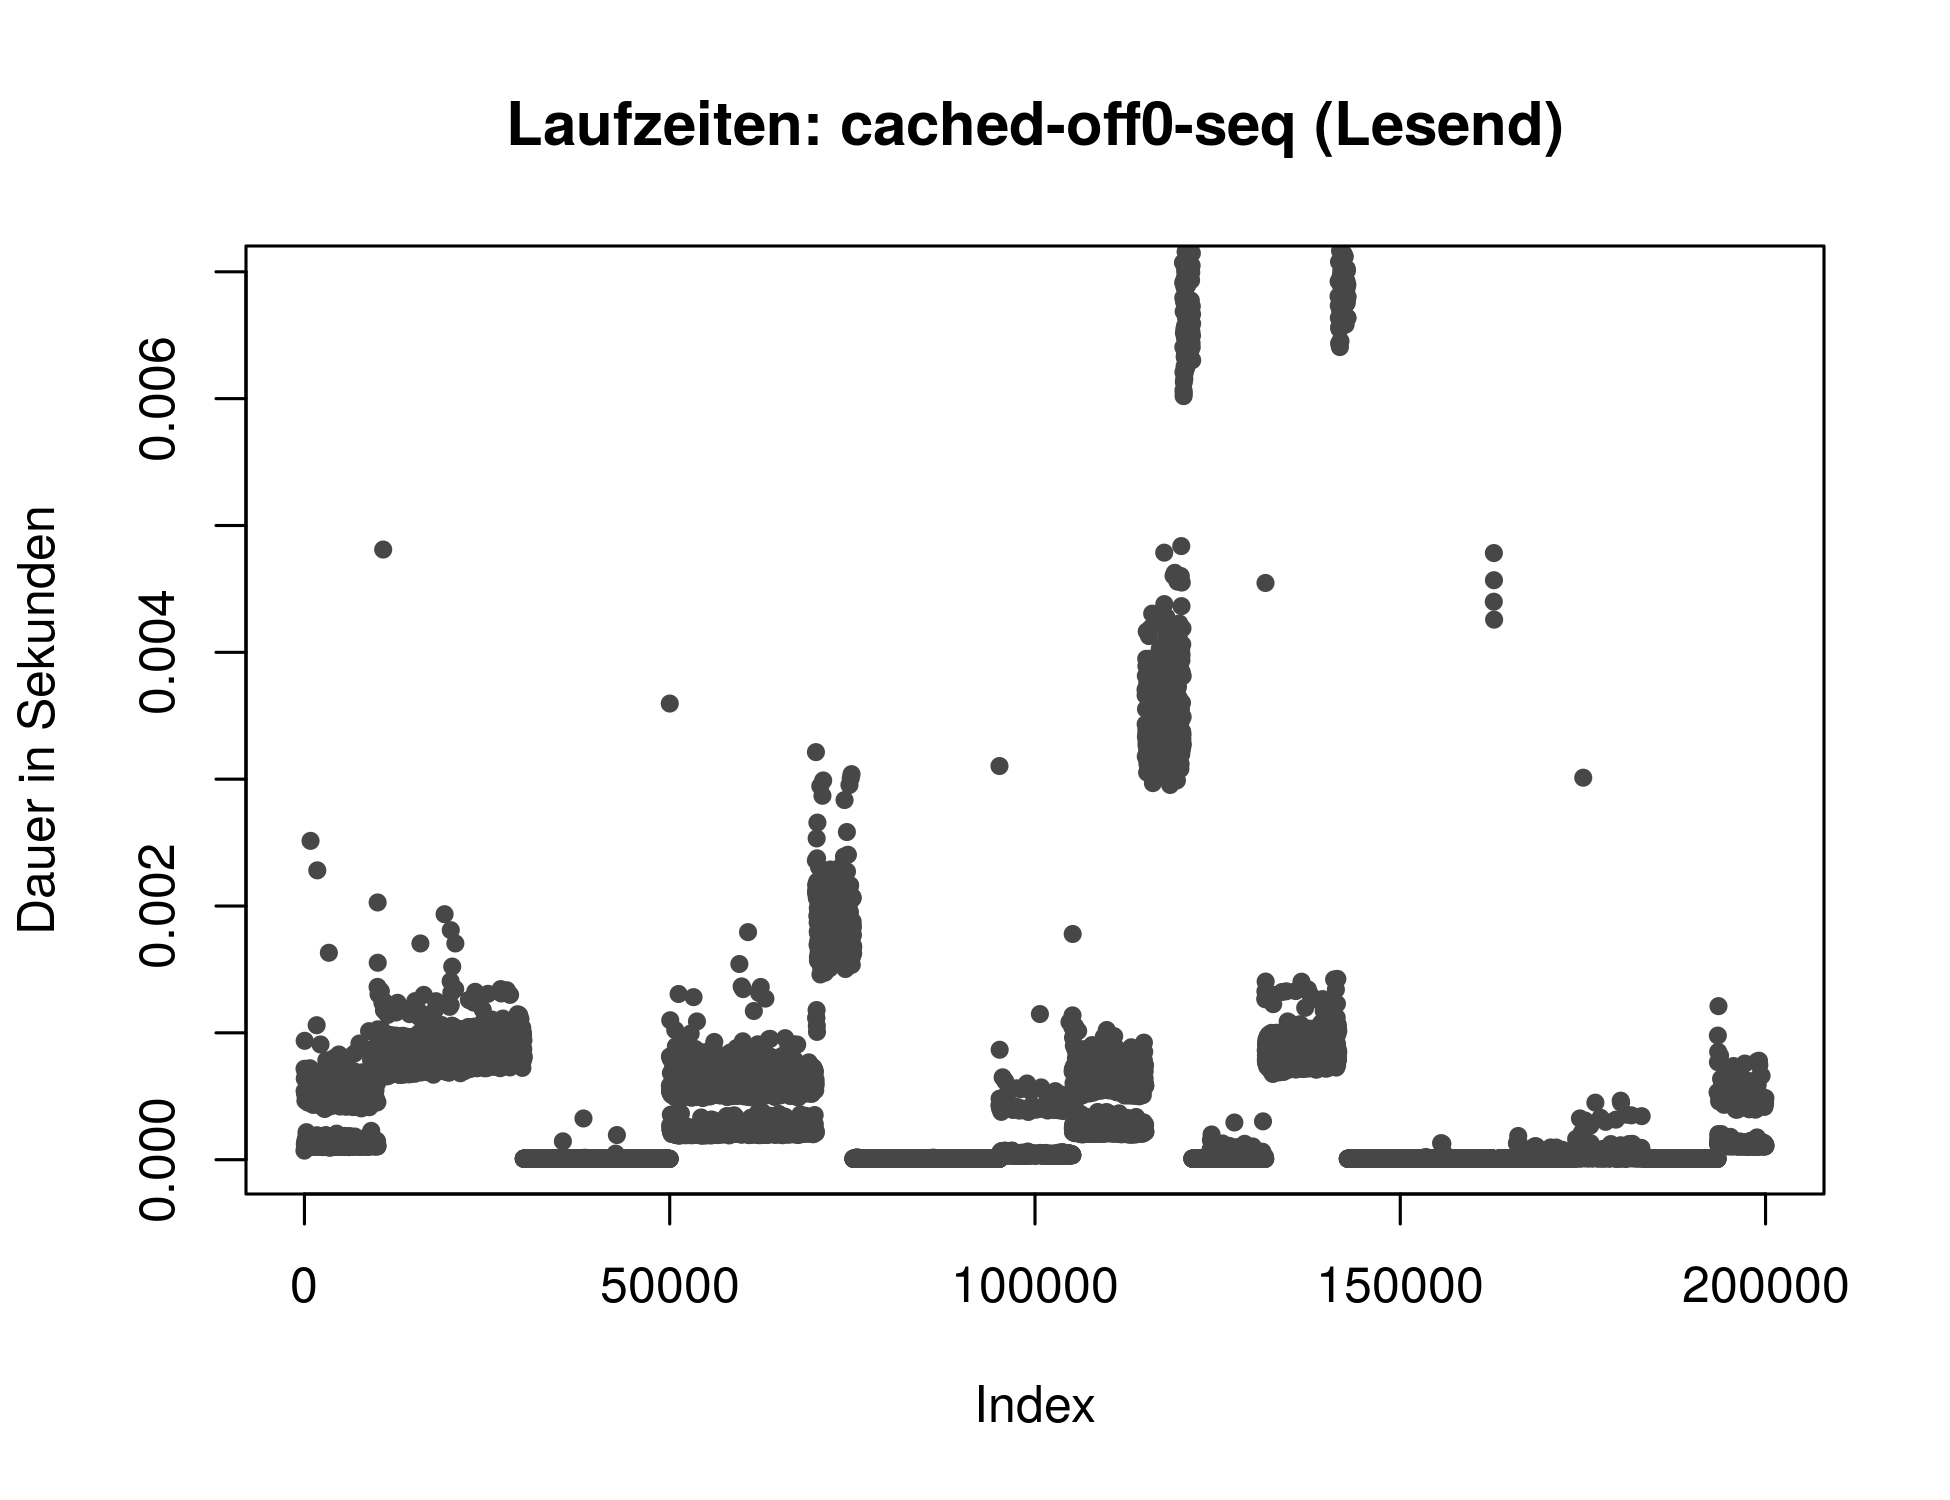
\includegraphics[width=.43\textwidth]{Bilder/Plots/exploration/plot_Duration_read_seq.png}
	}
	\hfill
	\subfloat{
		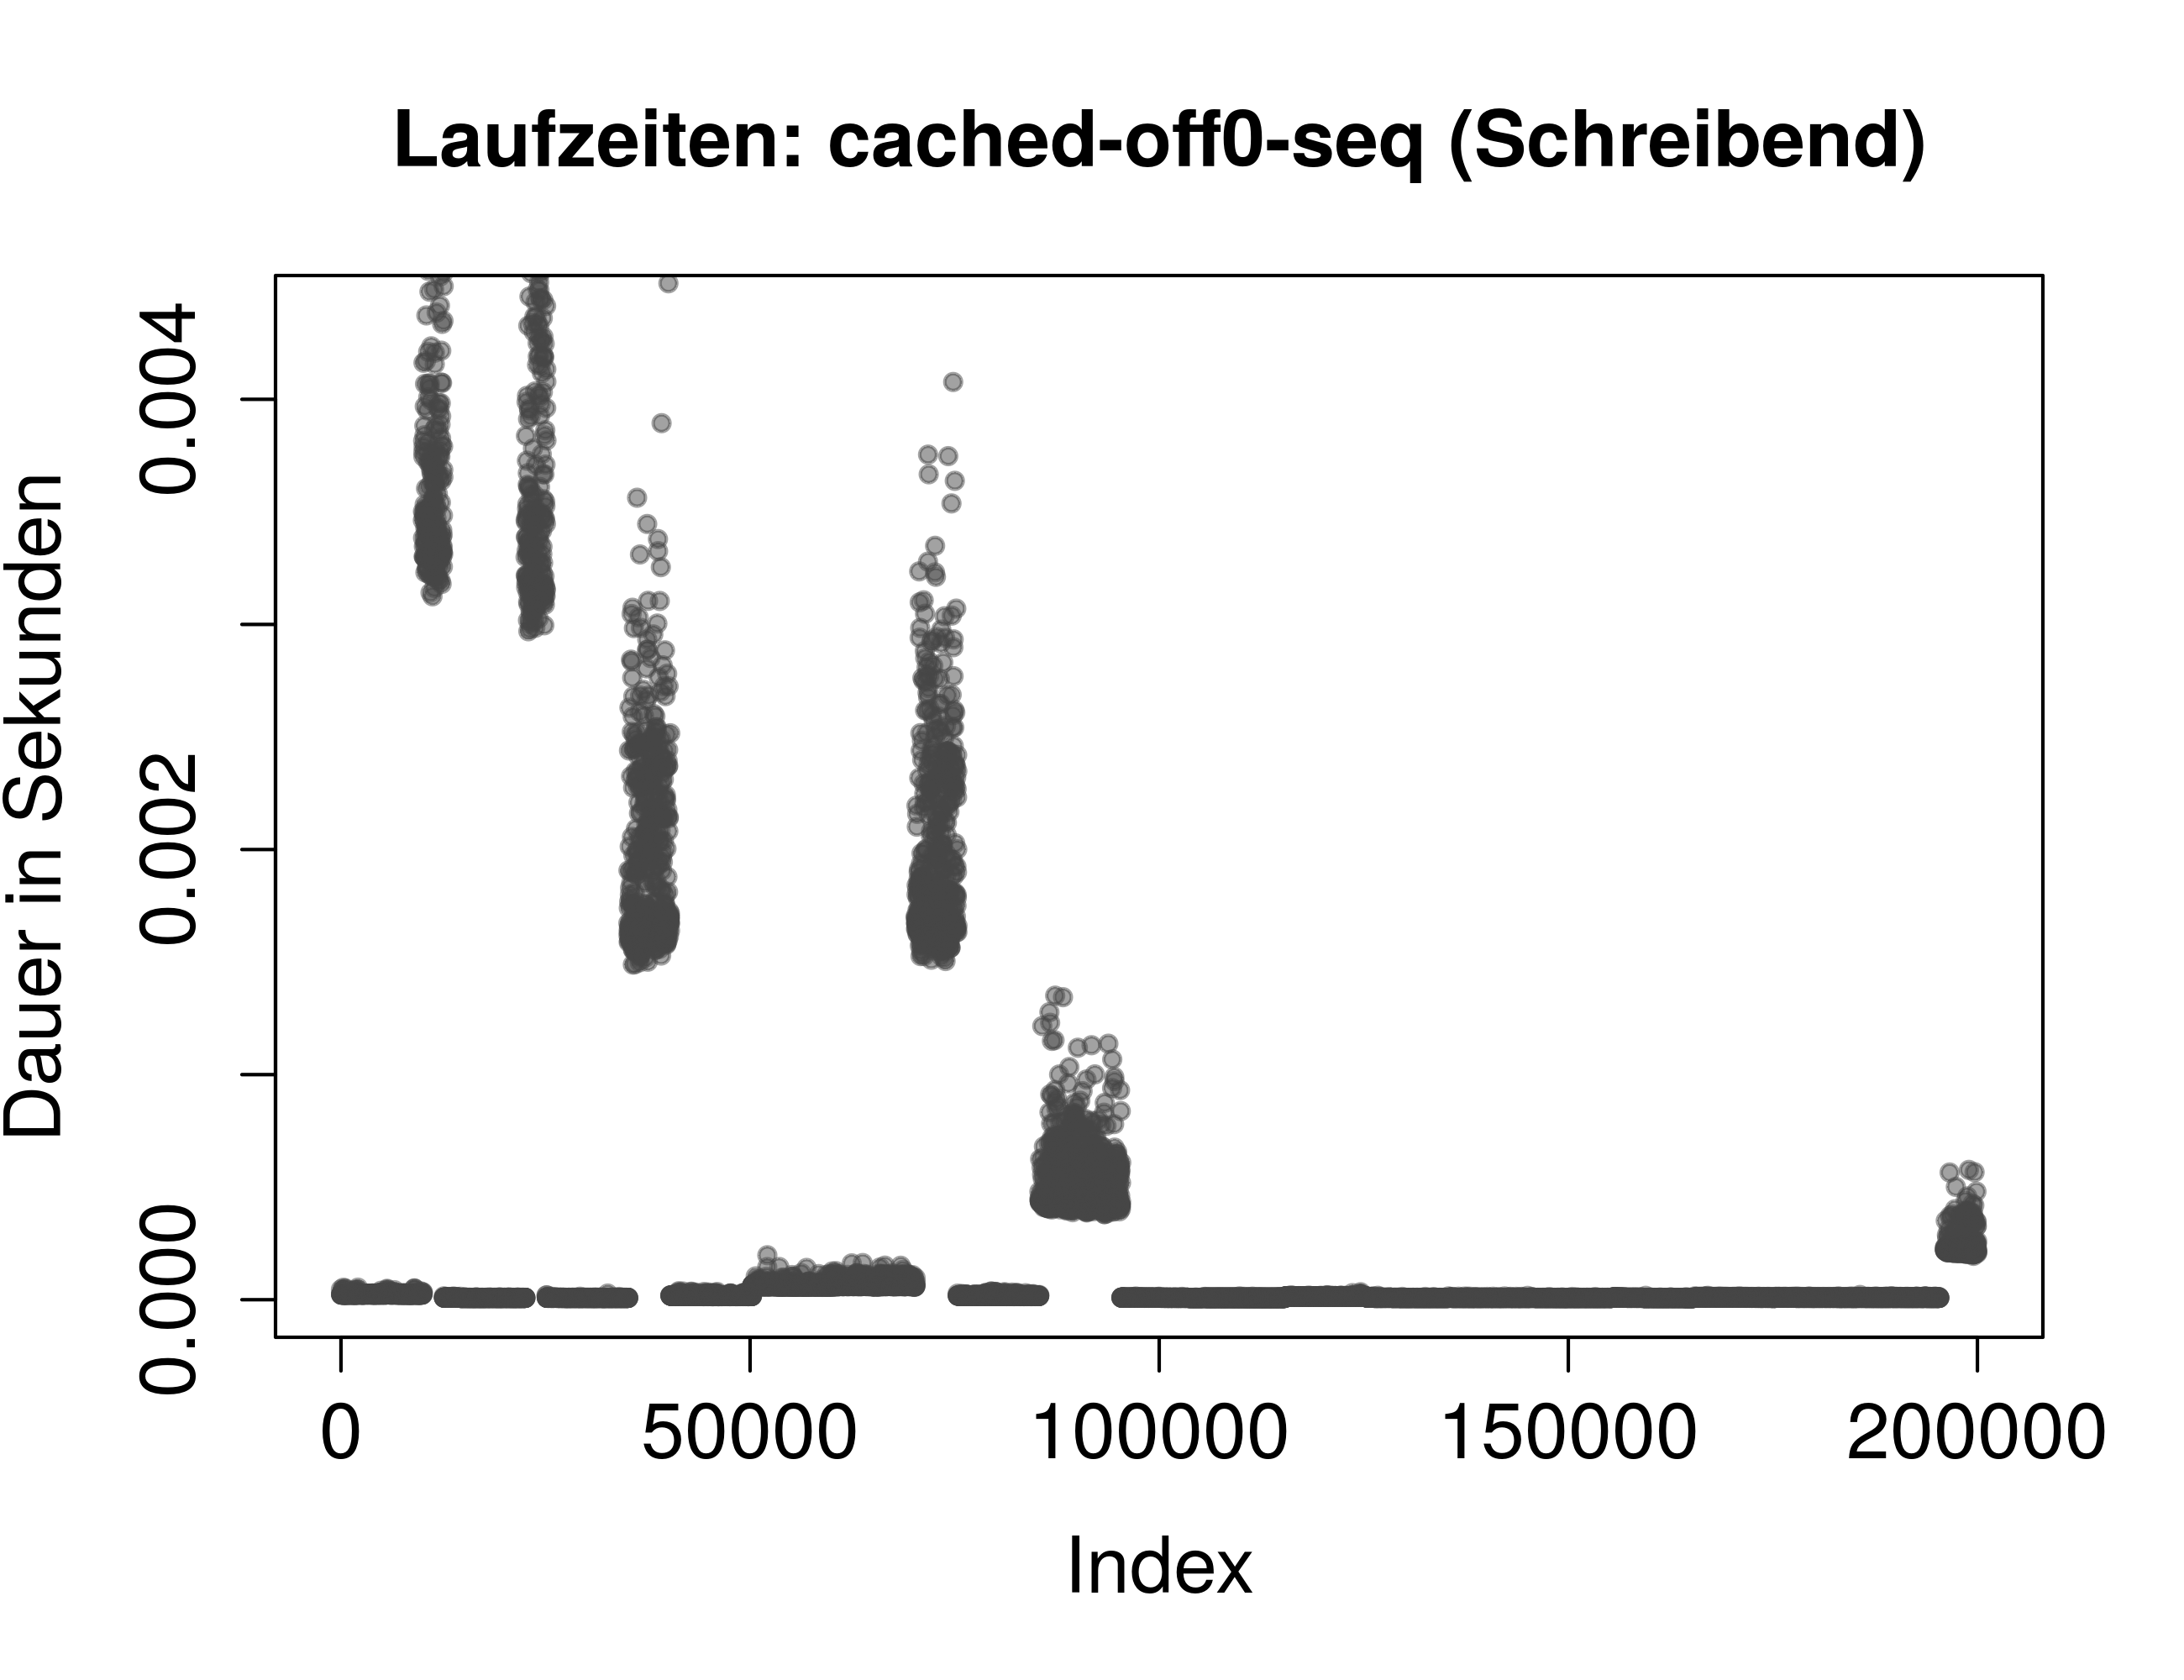
\includegraphics[width=.43\textwidth]{Bilder/Plots/exploration/plot_Duration_write_seq.png}
	}\\
	\subfloat{
		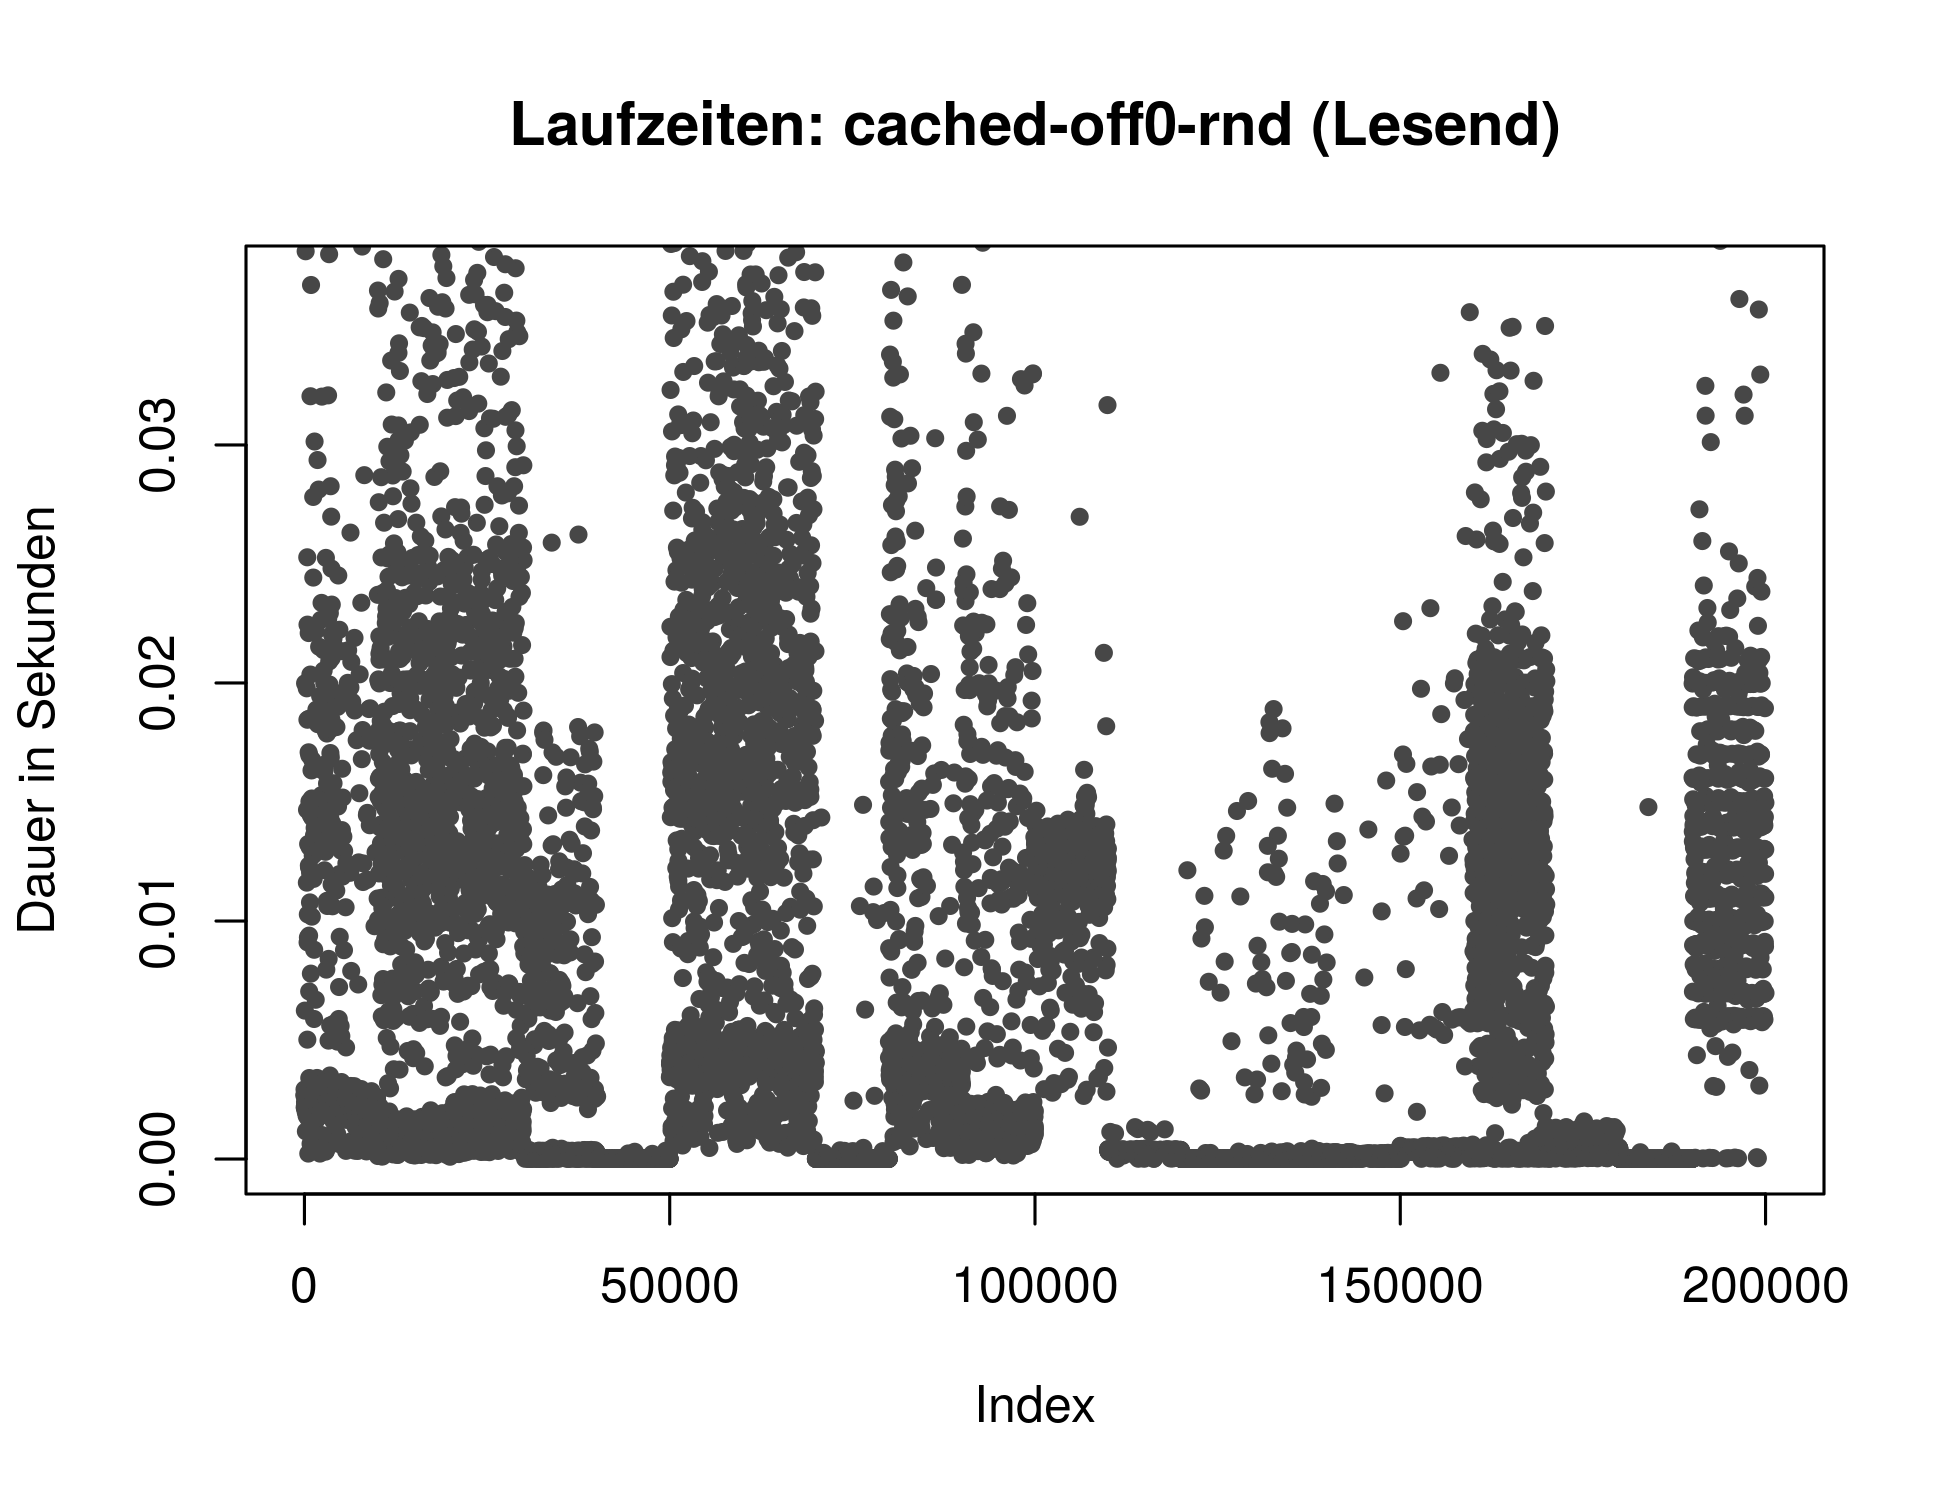
\includegraphics[width=.43\textwidth]{Bilder/Plots/exploration/plot_Duration_read_rnd.png}
	}
	\hfill
	\subfloat{
		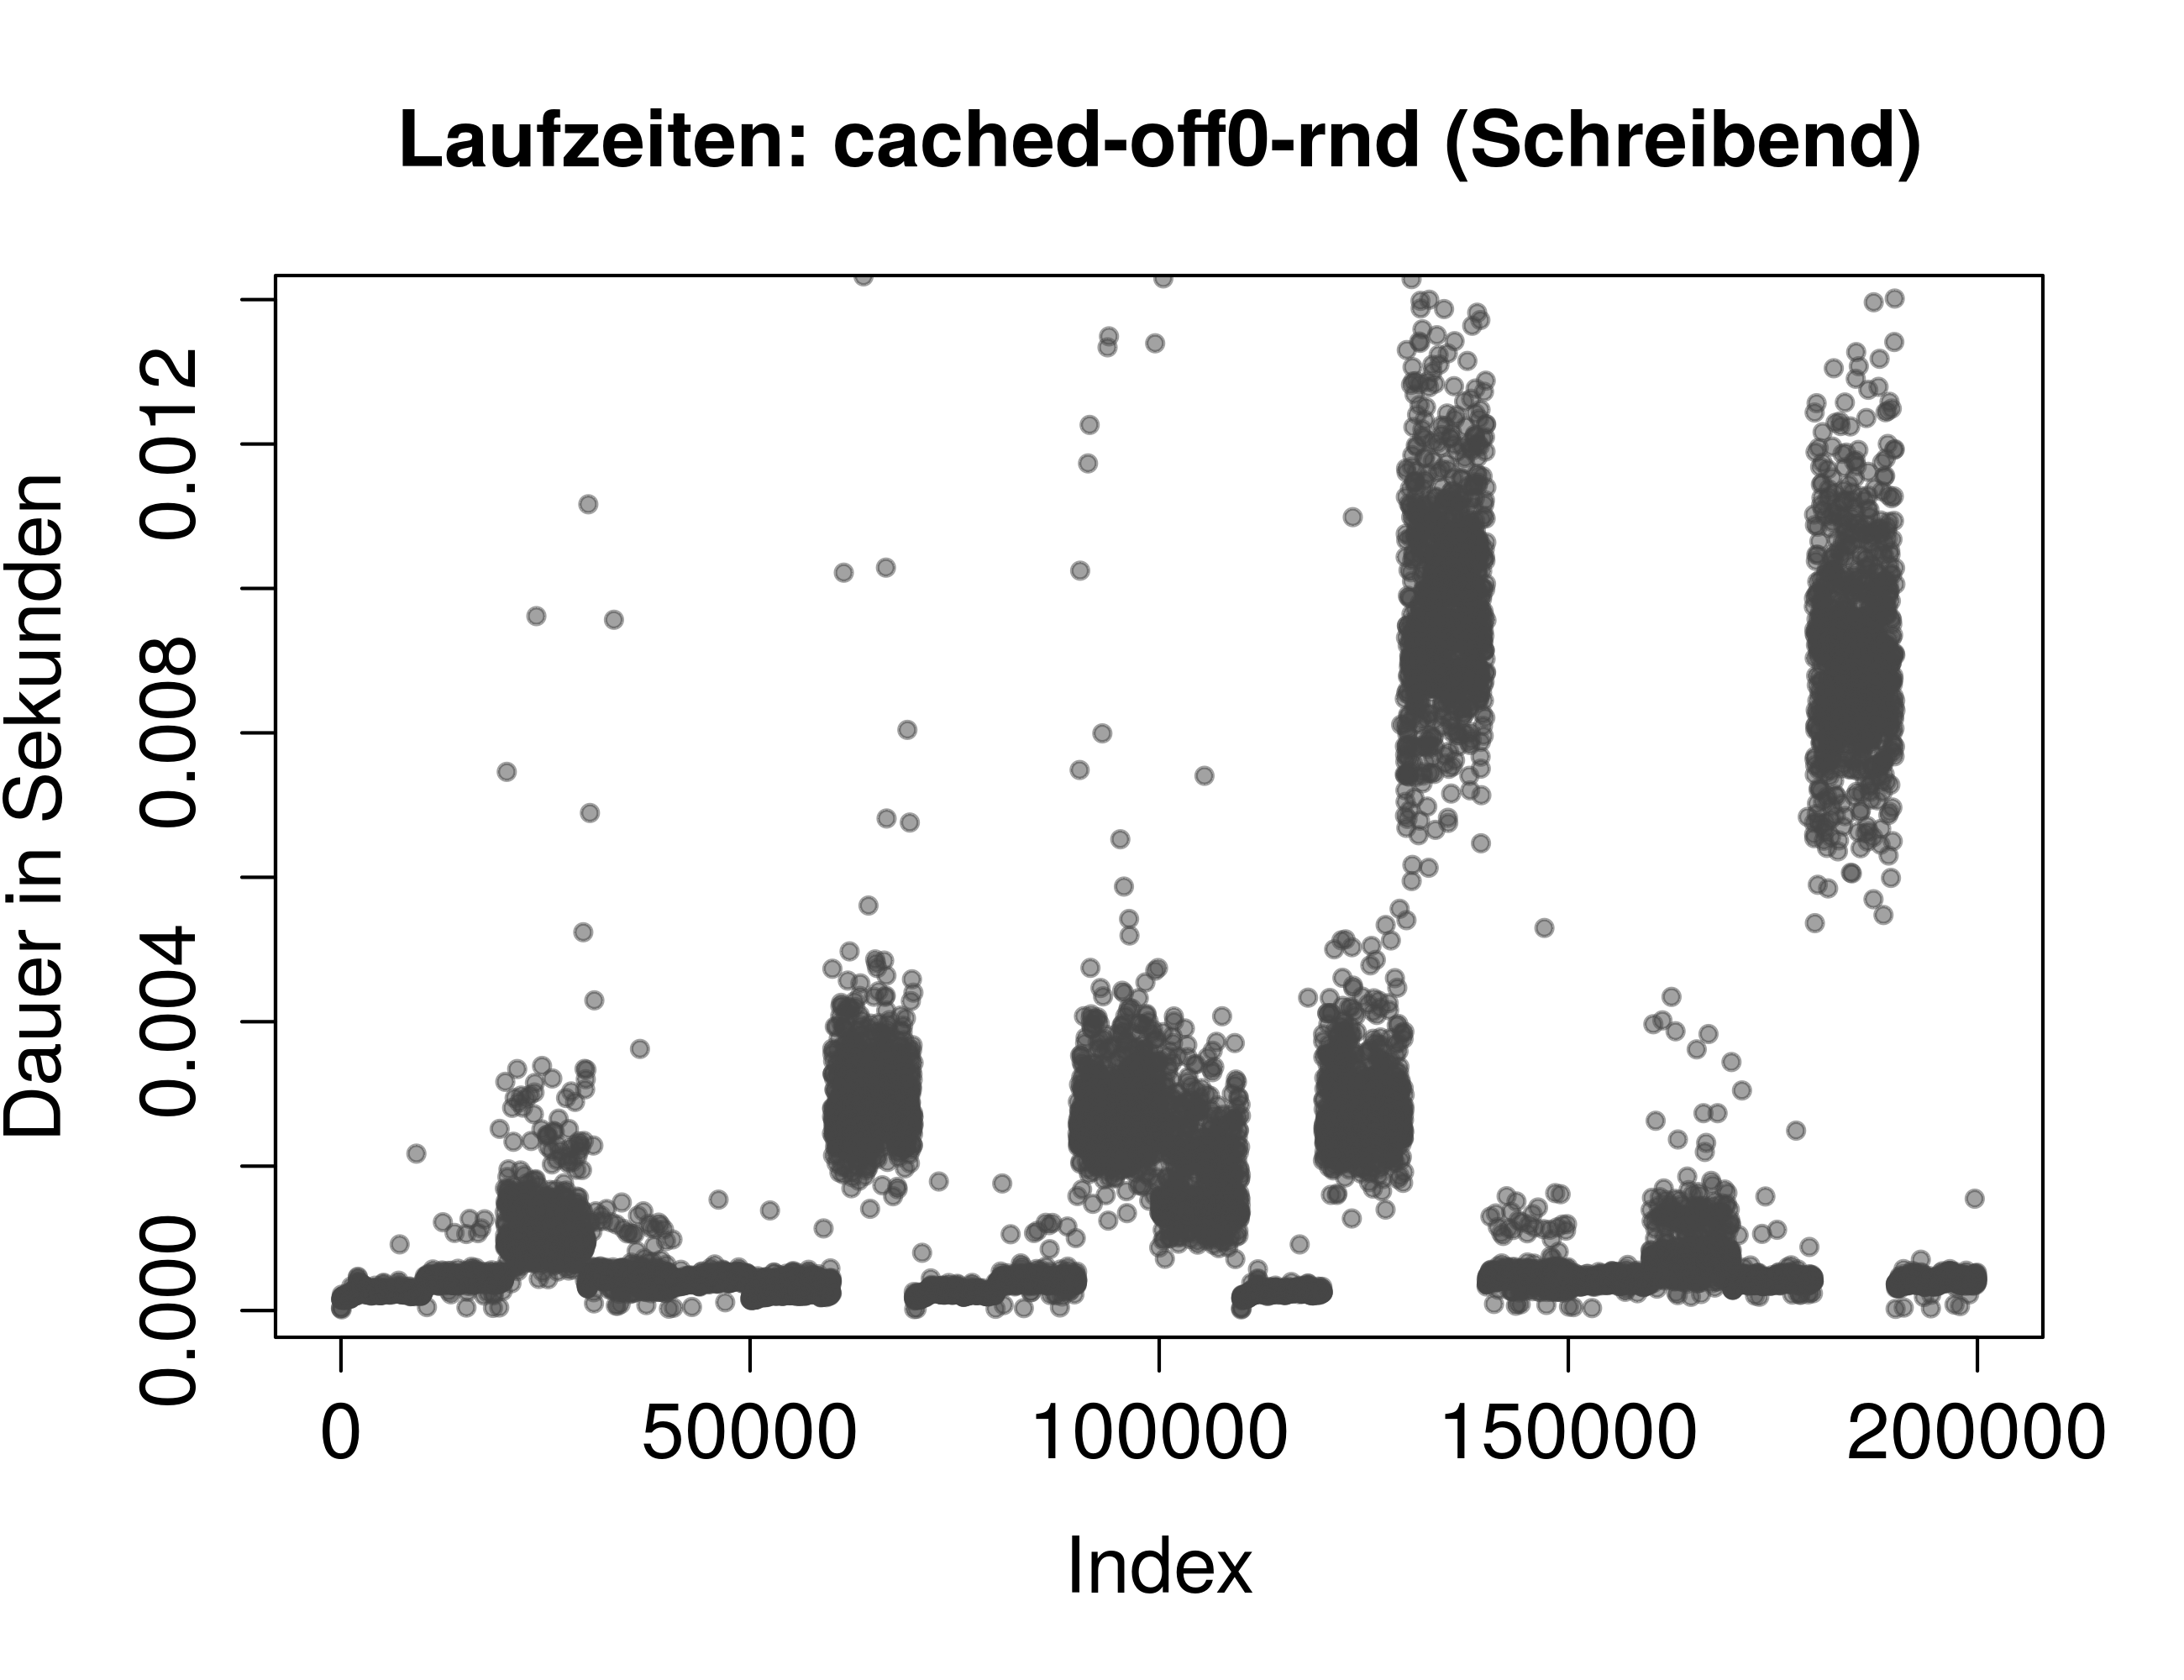
\includegraphics[width=.43\textwidth]{Bilder/Plots/exploration/plot_Duration_write_rnd.png}
	}		
	\caption{Messungen der Laufzeiten als Zeitreihe dargestellt, Index ist die Nummer der Messung}
	\label{Laufzeiten_Zeitreihe}
\end{figure} 

Wenn die Messpunkte nach der Laufzeit sortiert sind, kann die Verteilung Daten besser betrachtet werden. Die logarithmische Skalierung der Y-Achse entzerrt die Punkte (\ref{Laufzeiten_Sortiert}).

\begin{figure}
	\subfloat{
		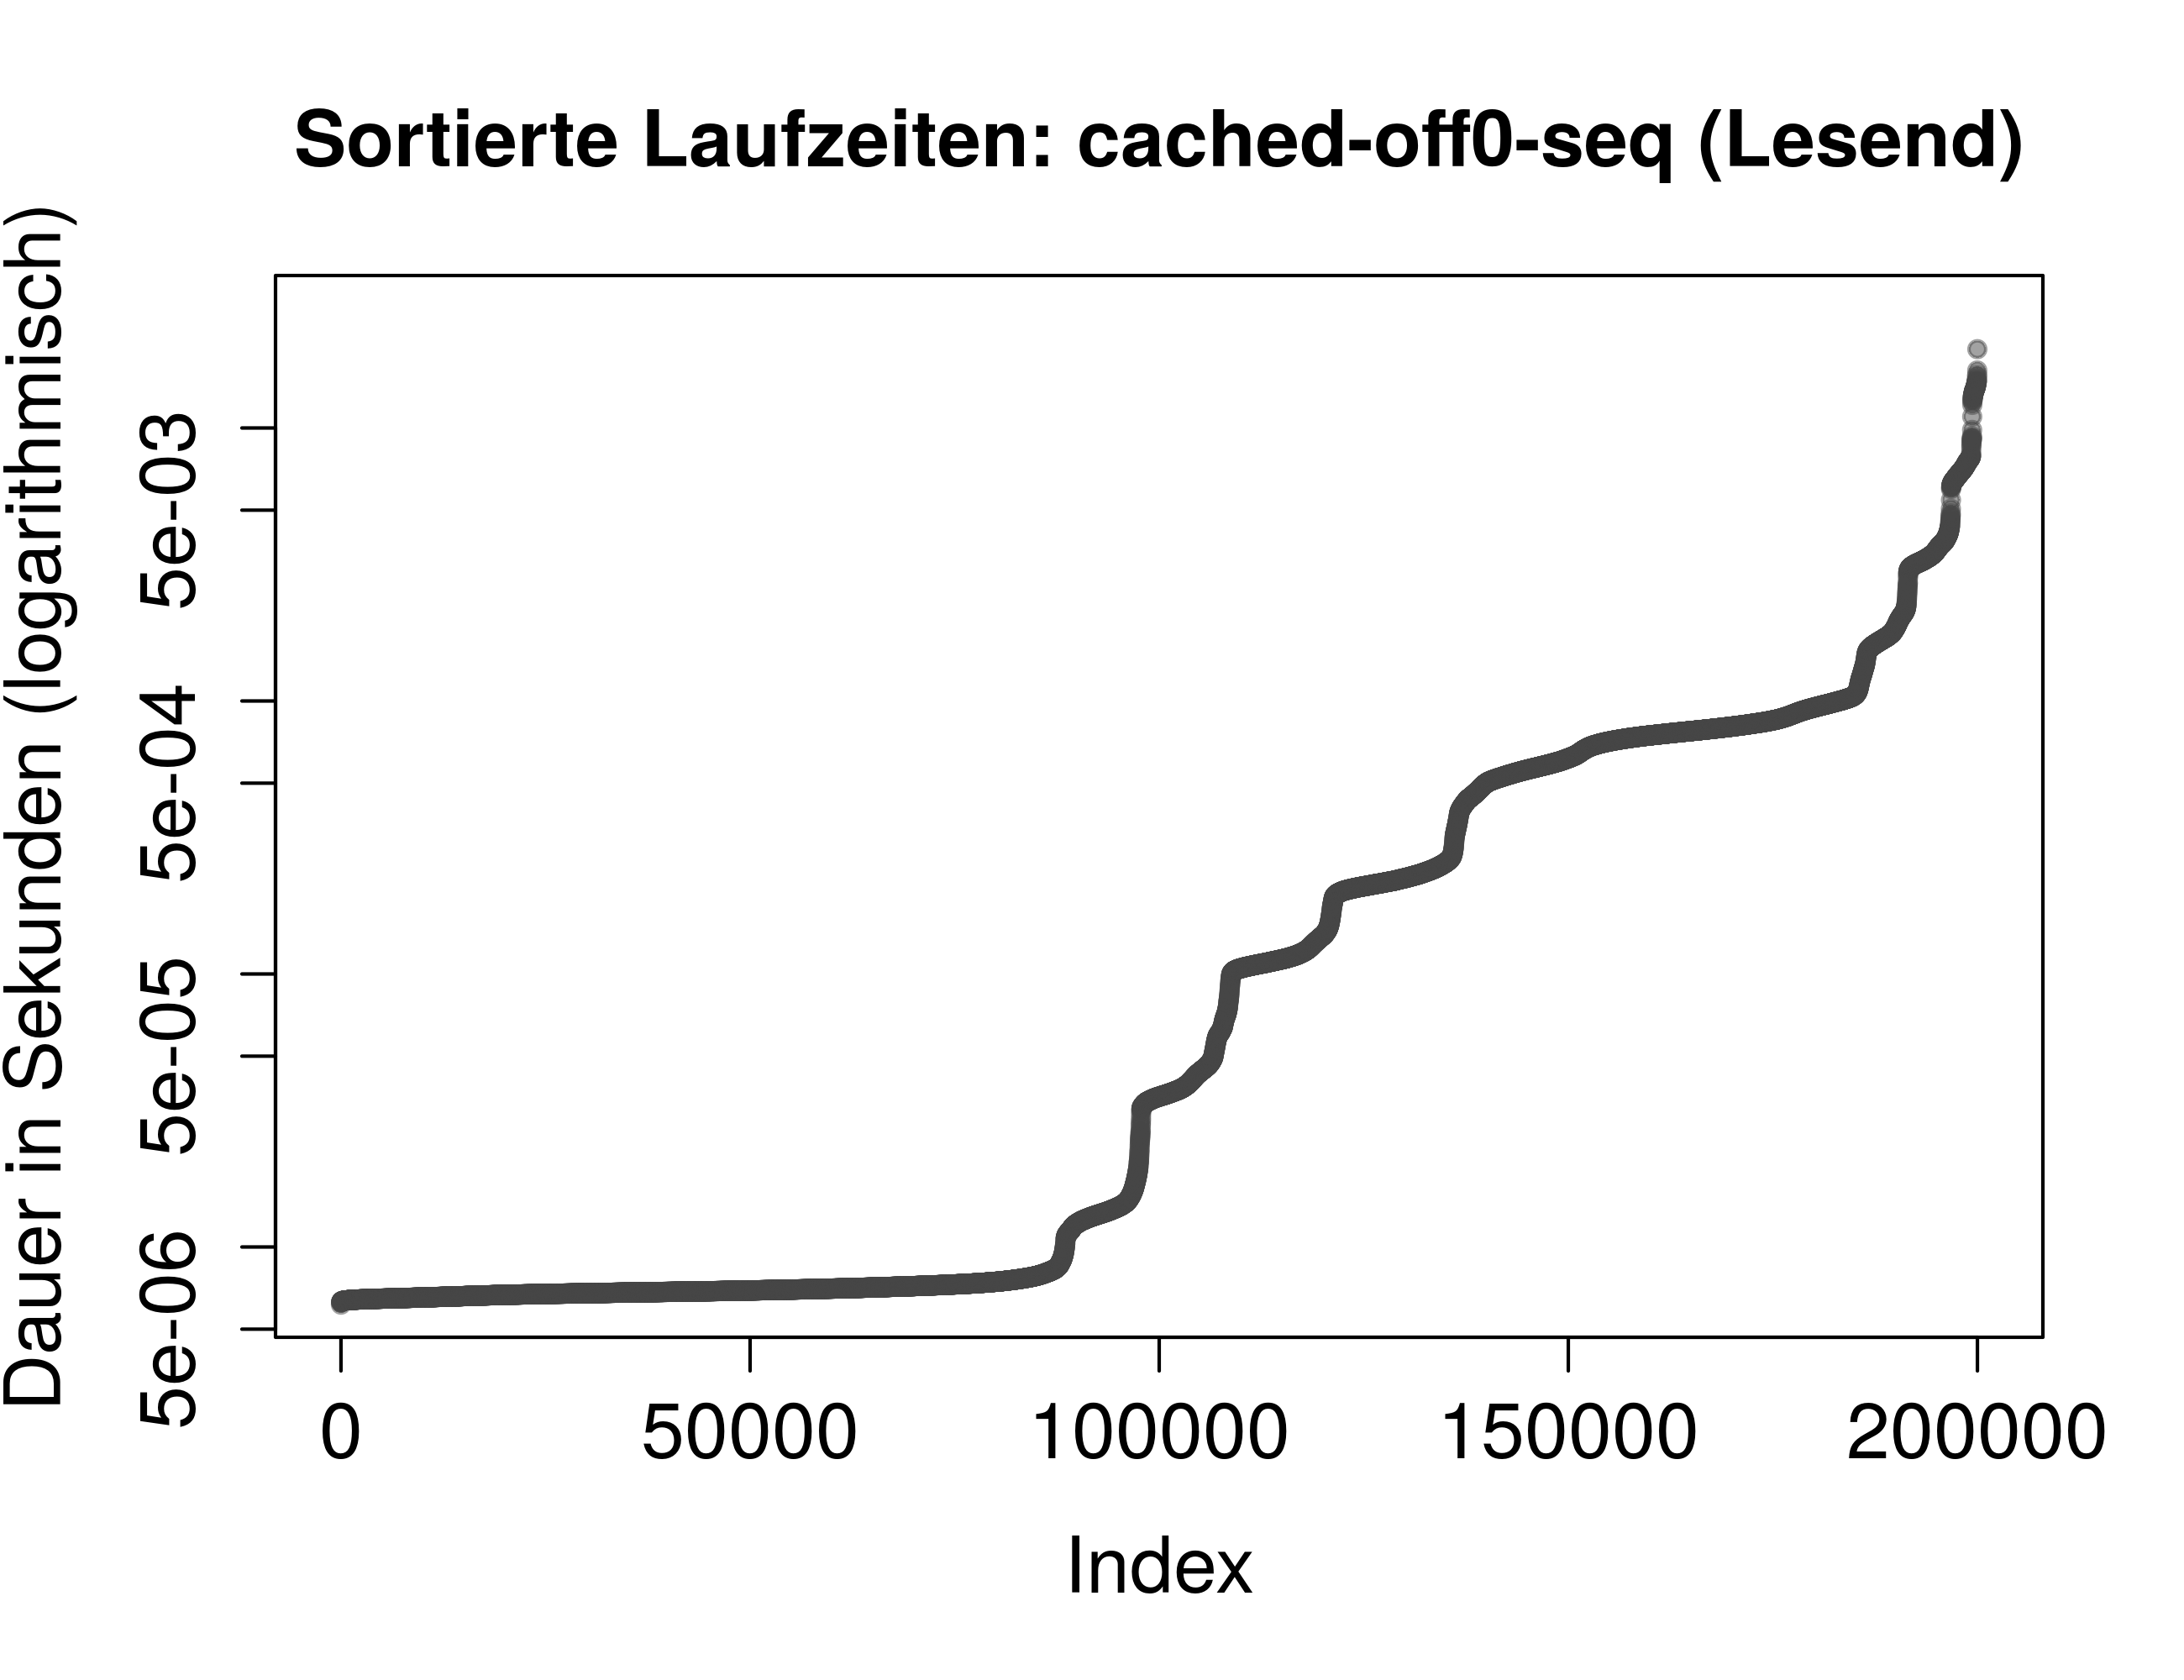
\includegraphics[width=.43\textwidth]{Bilder/Plots/exploration/plot_DurationSorted_read_seq.png}
	}
	\hfill
	\subfloat{
		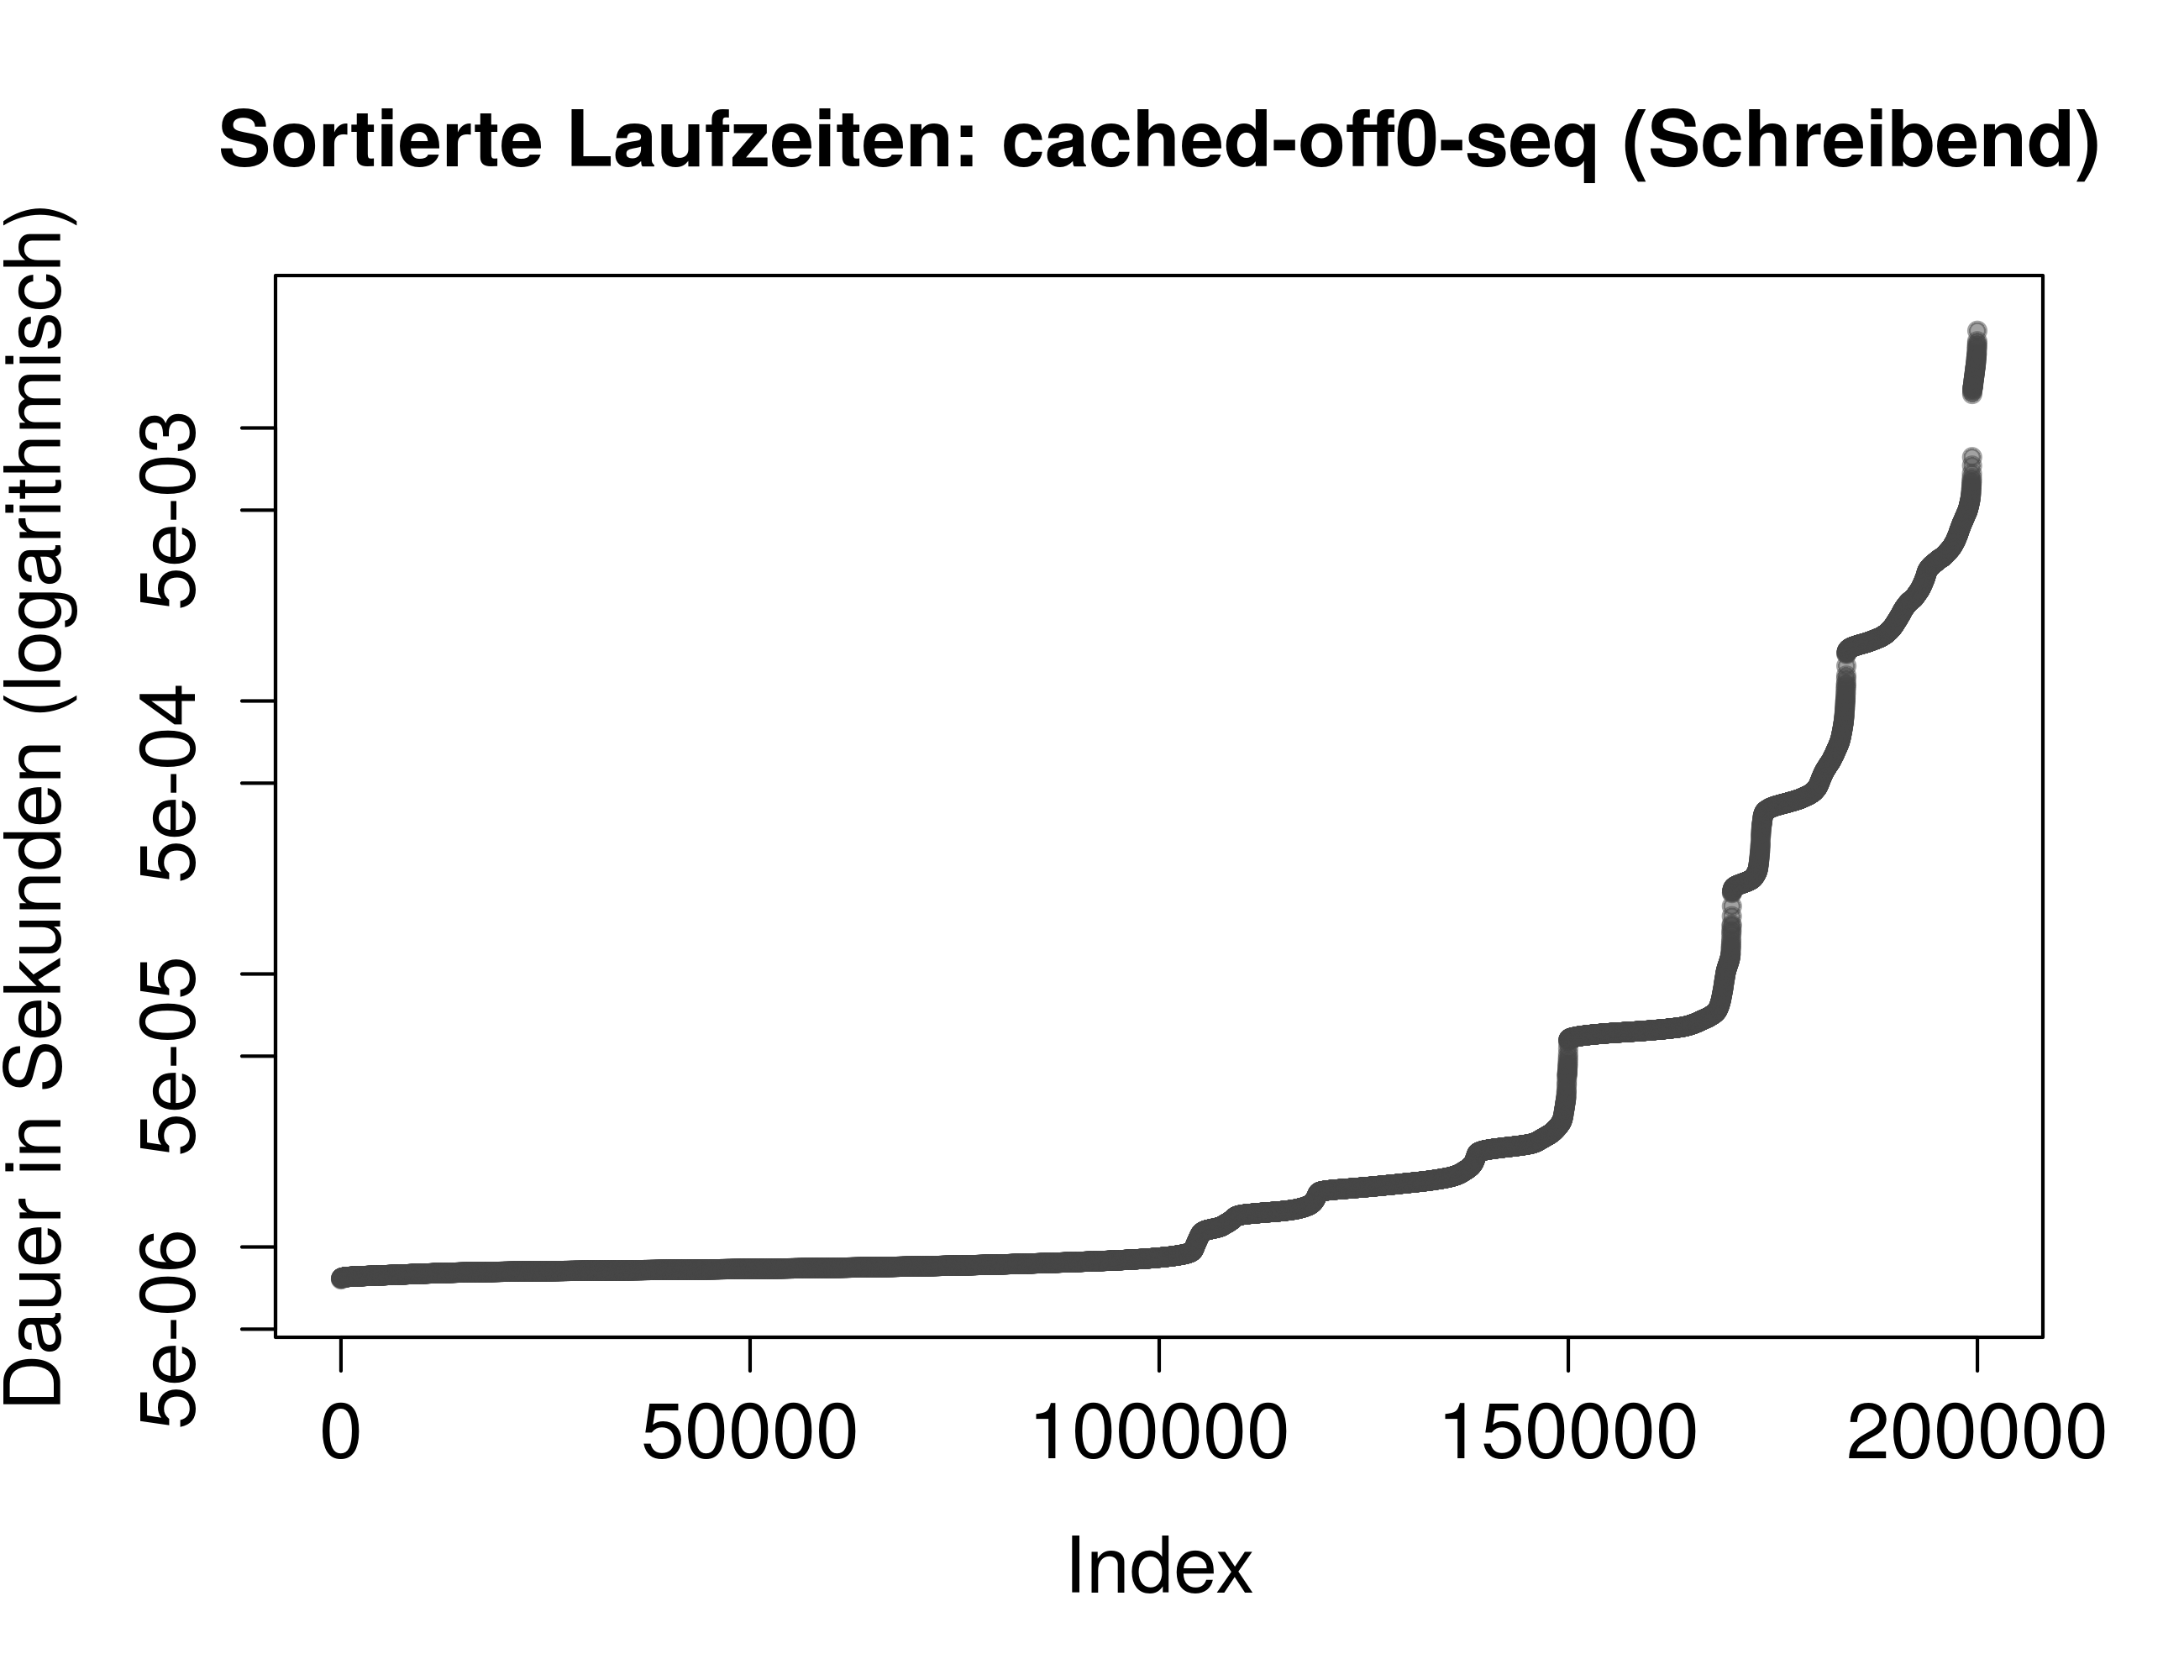
\includegraphics[width=.43\textwidth]{Bilder/Plots/exploration/plot_DurationSorted_write_seq.png}
	}\\
	\subfloat{
		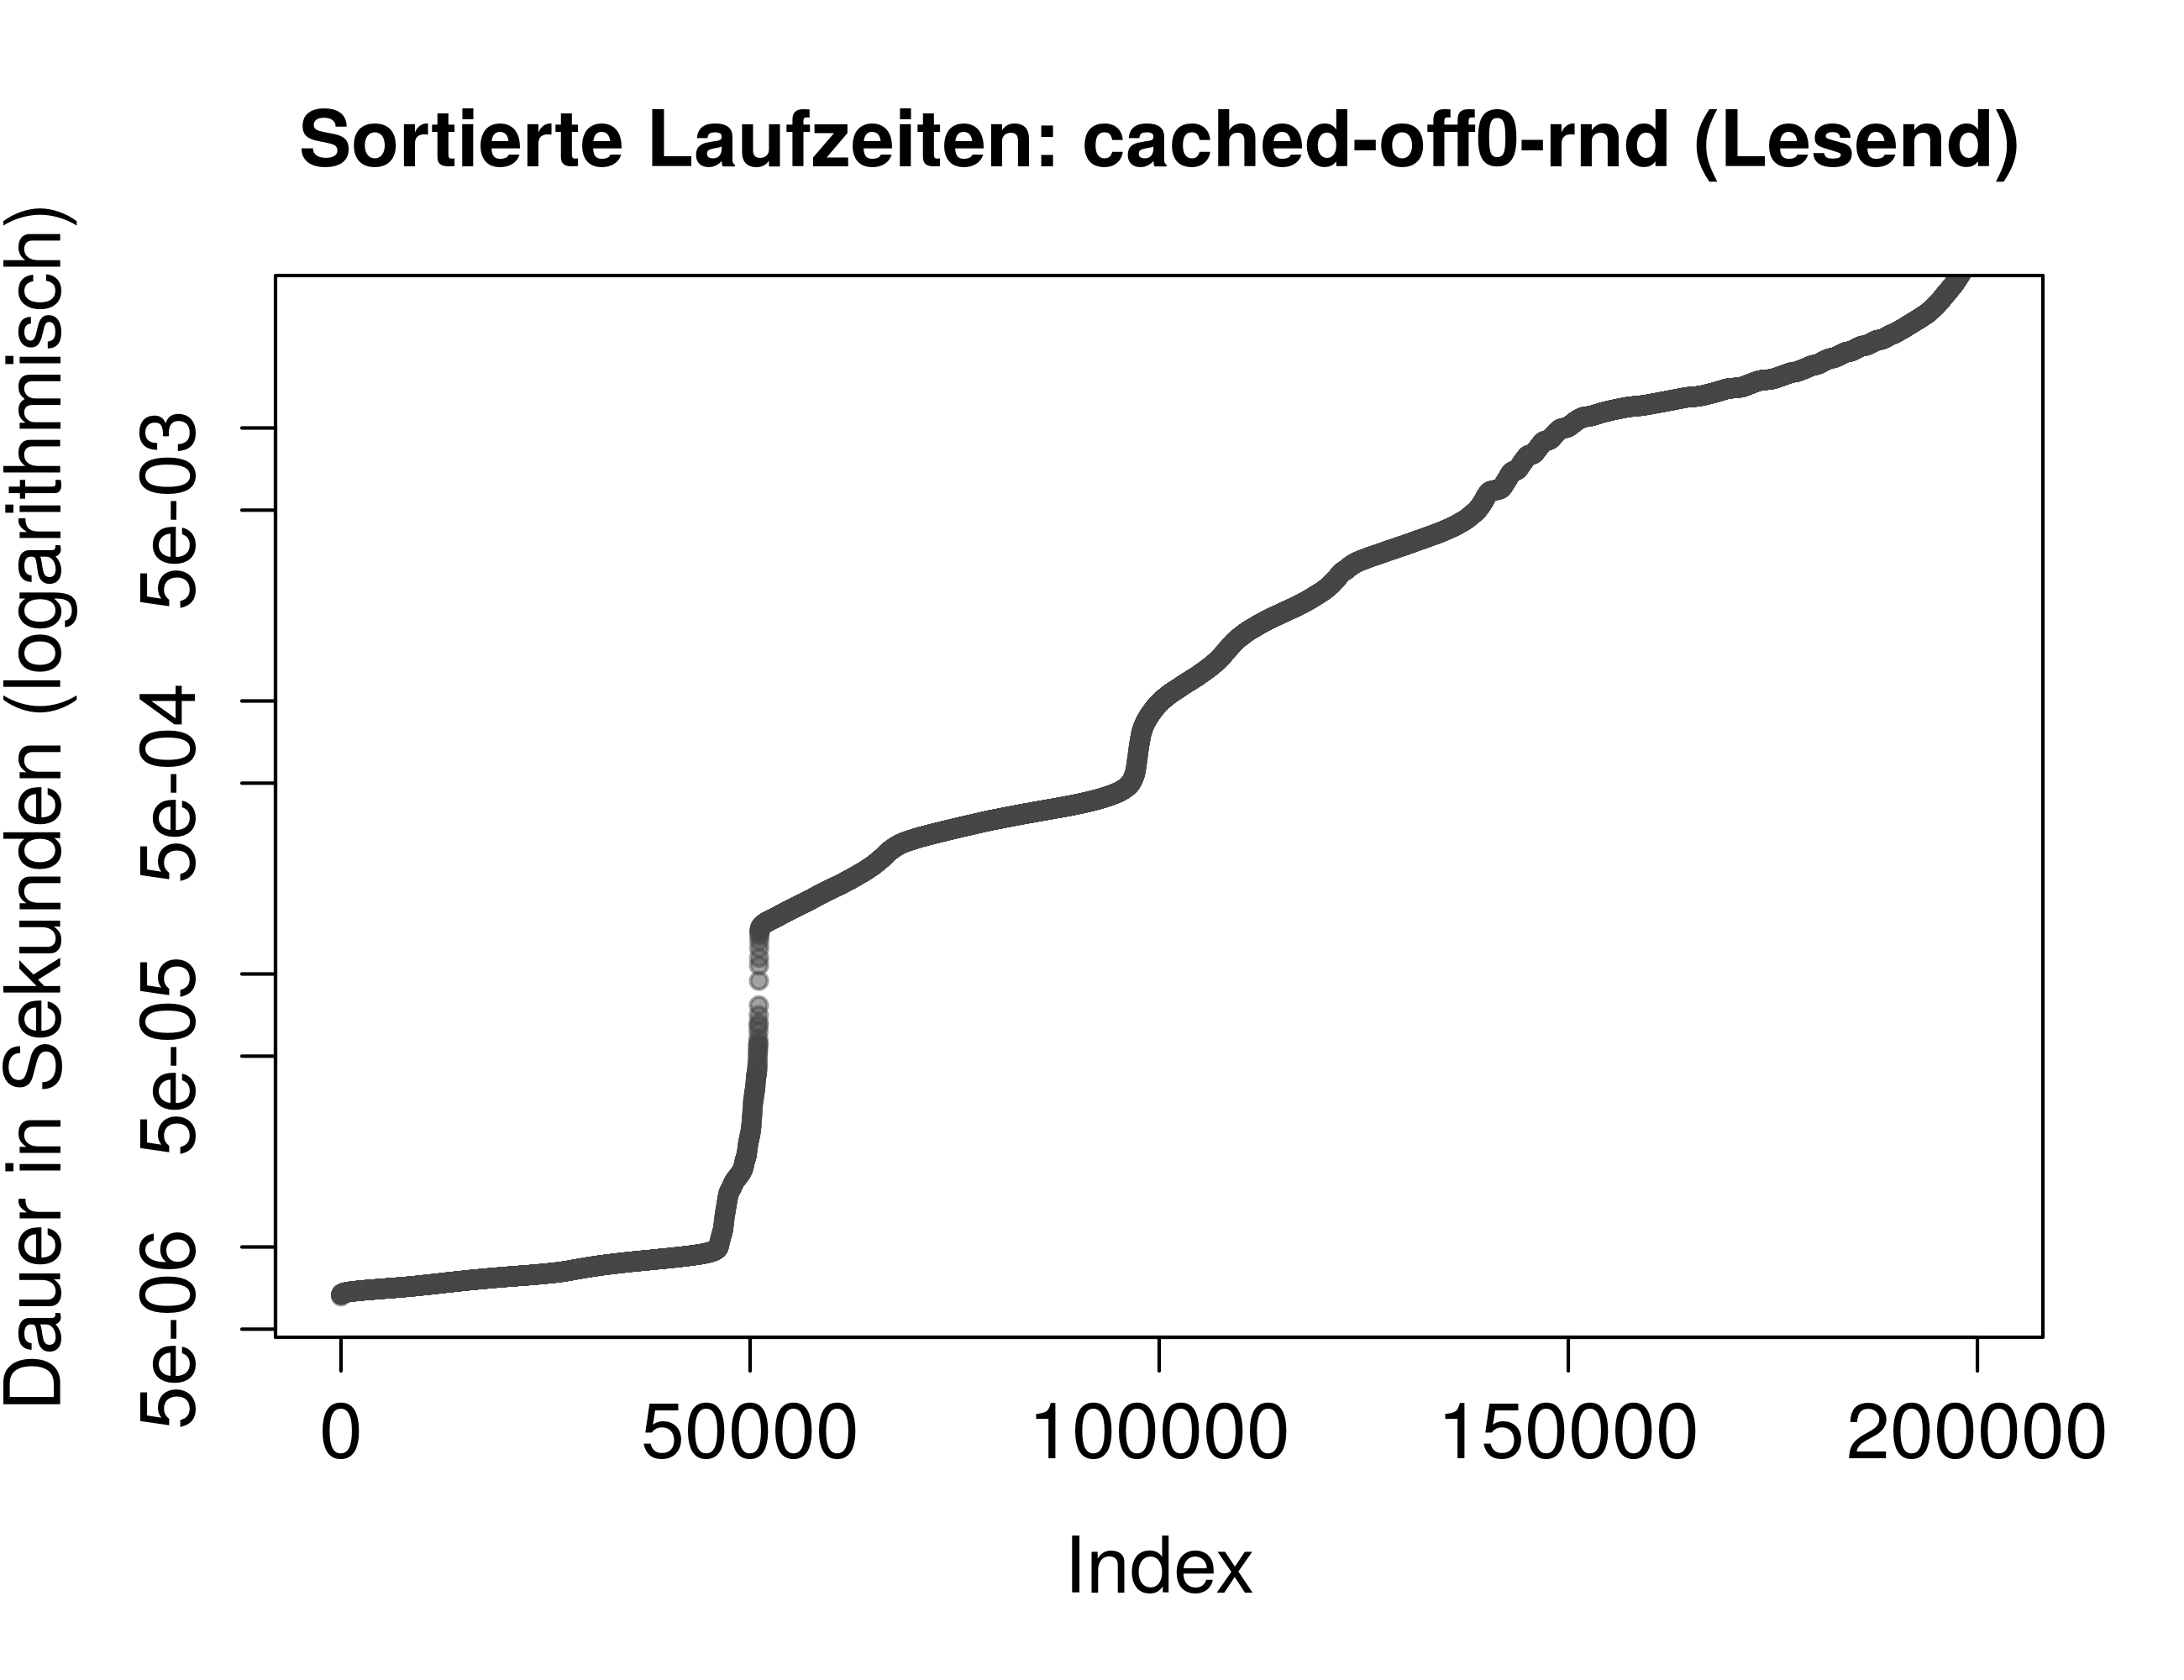
\includegraphics[width=.43\textwidth]{Bilder/Plots/exploration/plot_DurationSorted_read_rnd.png}
	}
	\hfill
	\subfloat{
		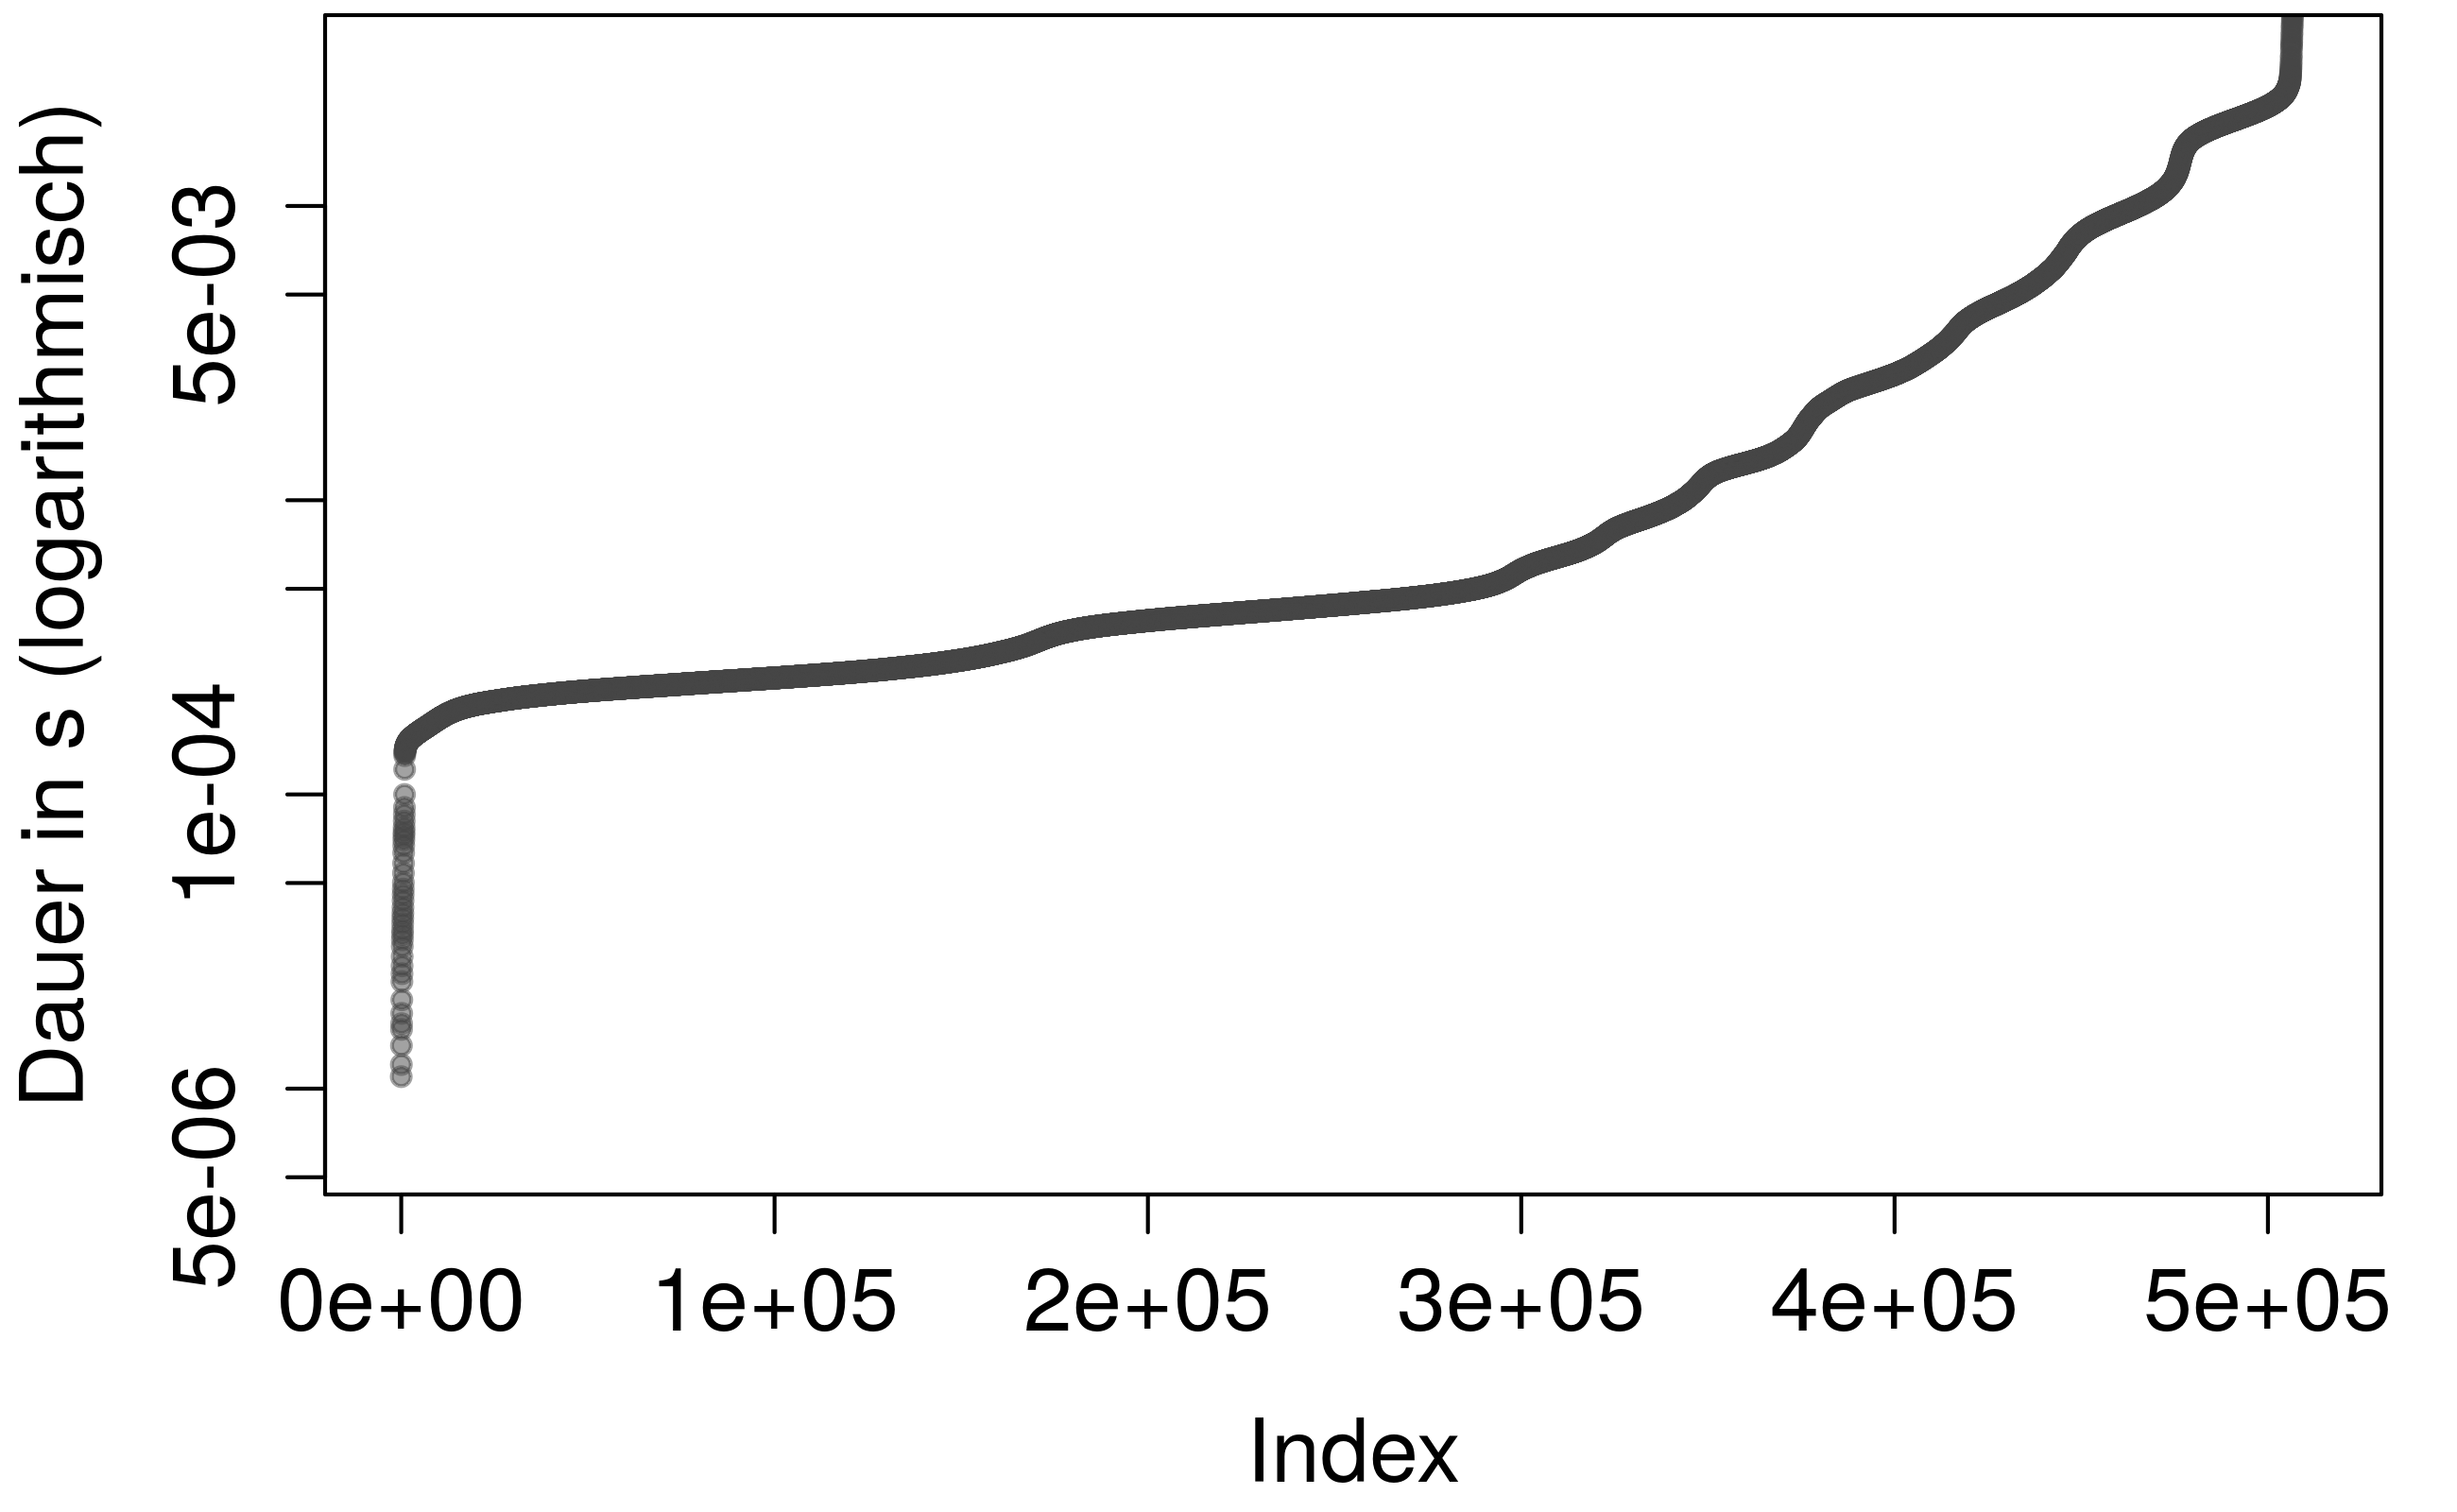
\includegraphics[width=.43\textwidth]{Bilder/Plots/exploration/plot_DurationSorted_write_rnd.png}
	}		
	\caption{Messungen der Laufzeiten sortiert dargestellt (logarithmische Y-Achse)}
	\label{Laufzeiten_Sortiert}
\end{figure} 

Zum Vergleich werden die Laufzeiten in \ref{Laufzeiten_Sortiert_nolog} ohne logarithmische Y-Achse dargestellt. Aufgrund der Häufung von Messungen mit sehr kurzer Laufzeit sind etwa die ersten 100.000 Werte in dieser Darstellung nicht zu unterscheiden. Aus diesem Grund werden die Laufzeiten (und Zugriffsgrößen zur Erhaltung der Korrelation) für die höheren Modelle zum Lernen logarithmiert. Da die neuronalen Netze versuchen den Modellfehler zu minimieren würde es ansonsten eine Tendenz dazu geben, die Messungen mit längerer Laufzeit korrekt zu lernen. Während für die kürzeren Laufzeiten für den internen Modellfehler unwichtiger wären. Ein ungenaues Lernen der Messungen mit kürzeren Laufzeiten würde sich  nicht in einer absoluten Metrik, sondern nur in einer Relativen niederschlagen.

\begin{figure}
	\subfloat{
		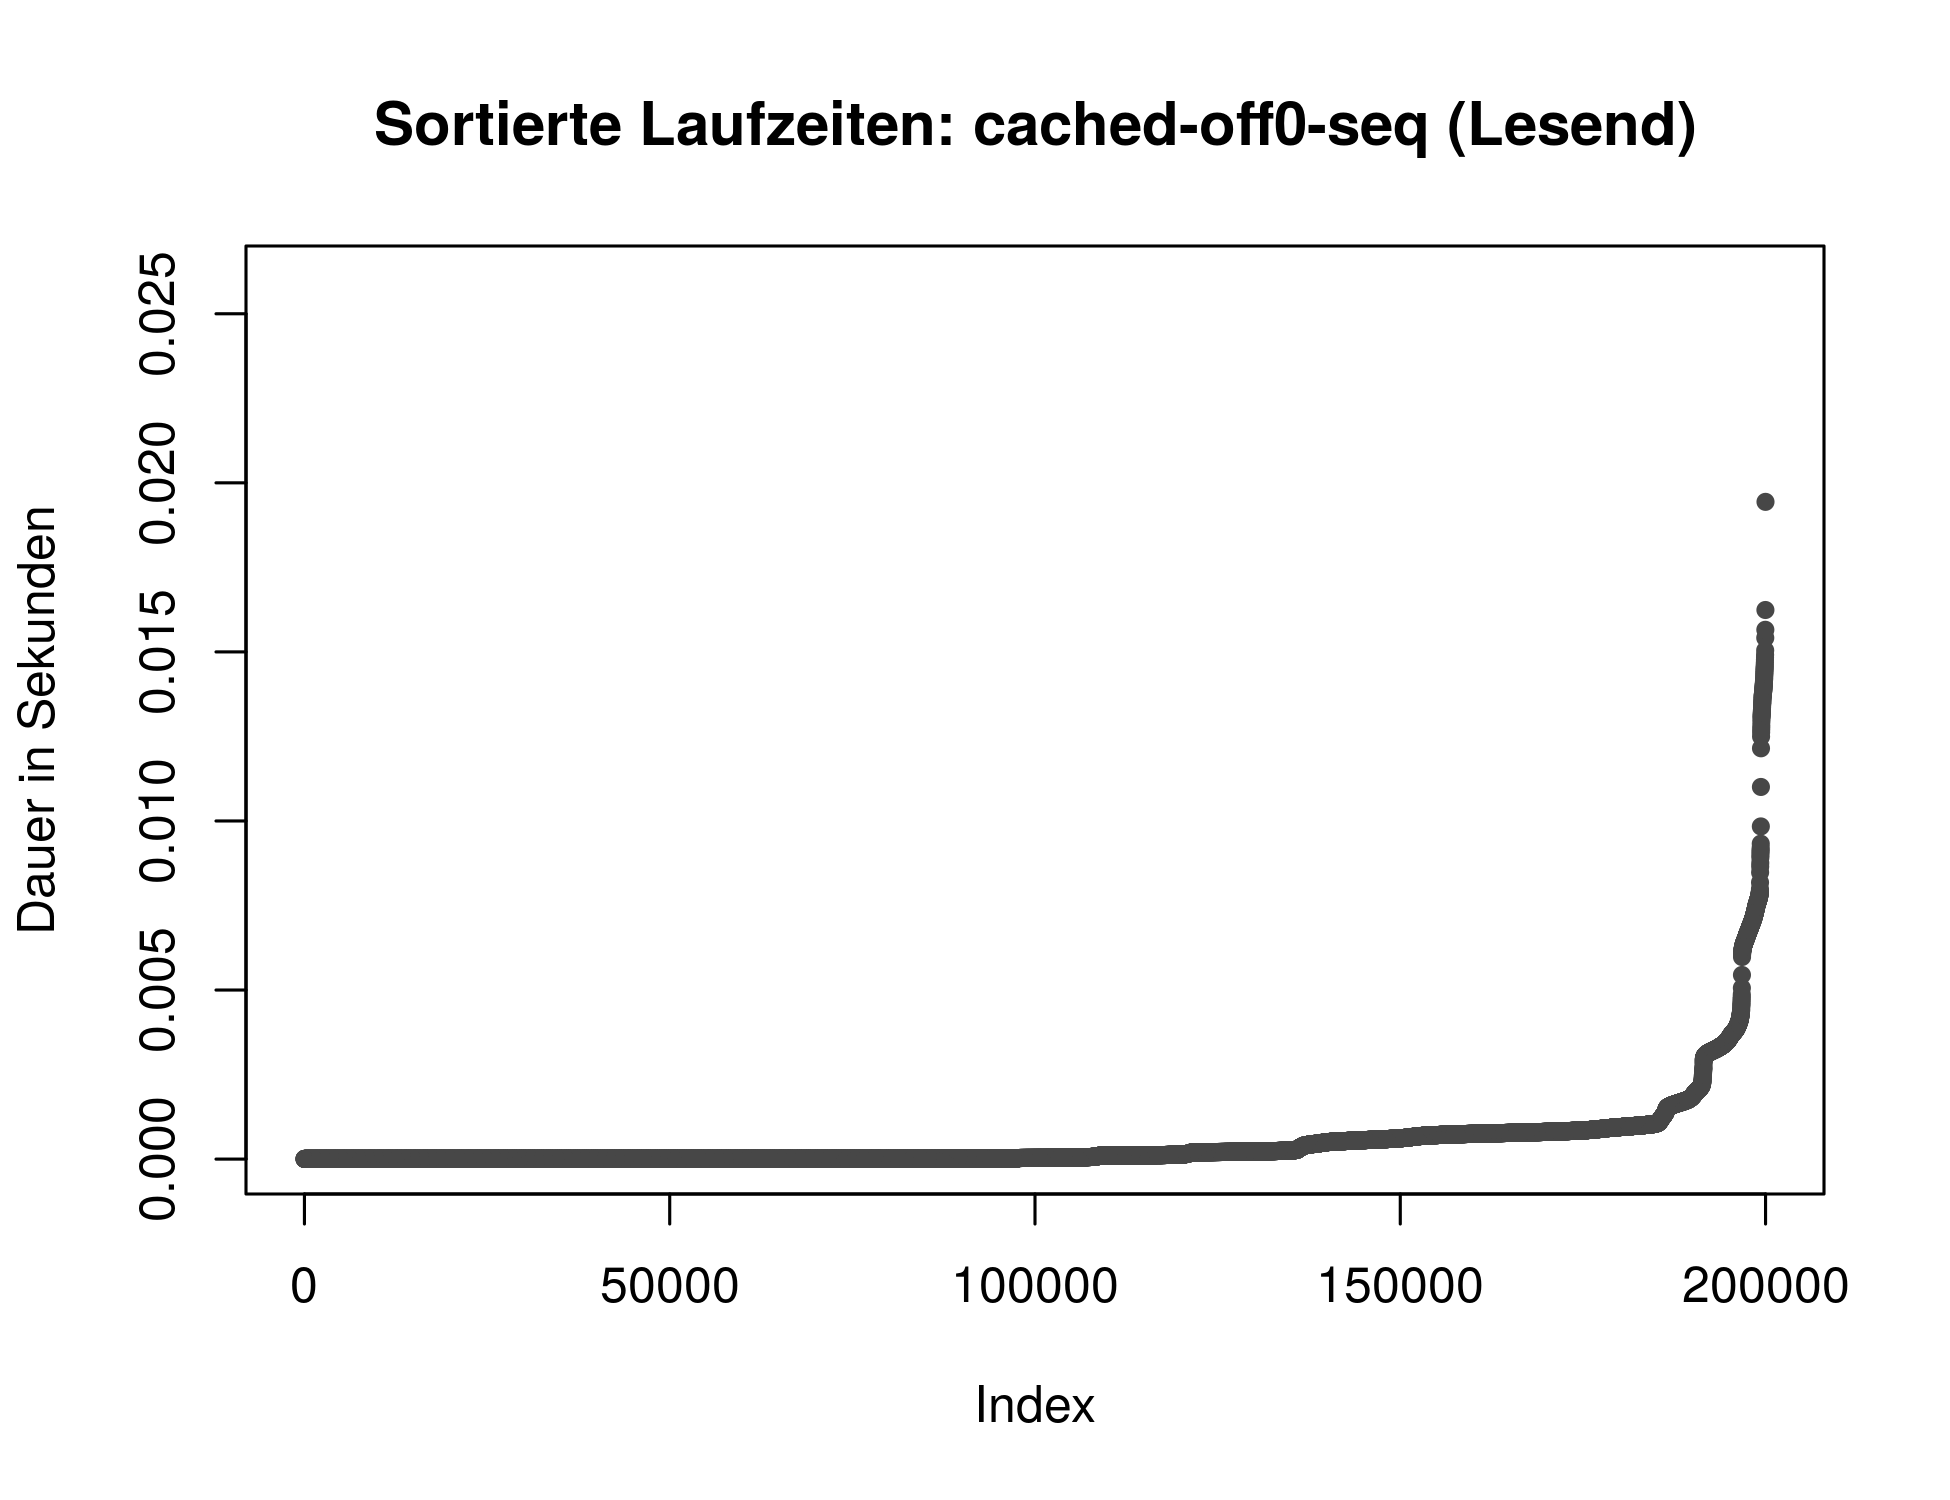
\includegraphics[width=.43\textwidth]{Bilder/Plots/exploration/plot_DurationSorted_read_seq_nolog.png}
	}
	\hfill
	\subfloat{
		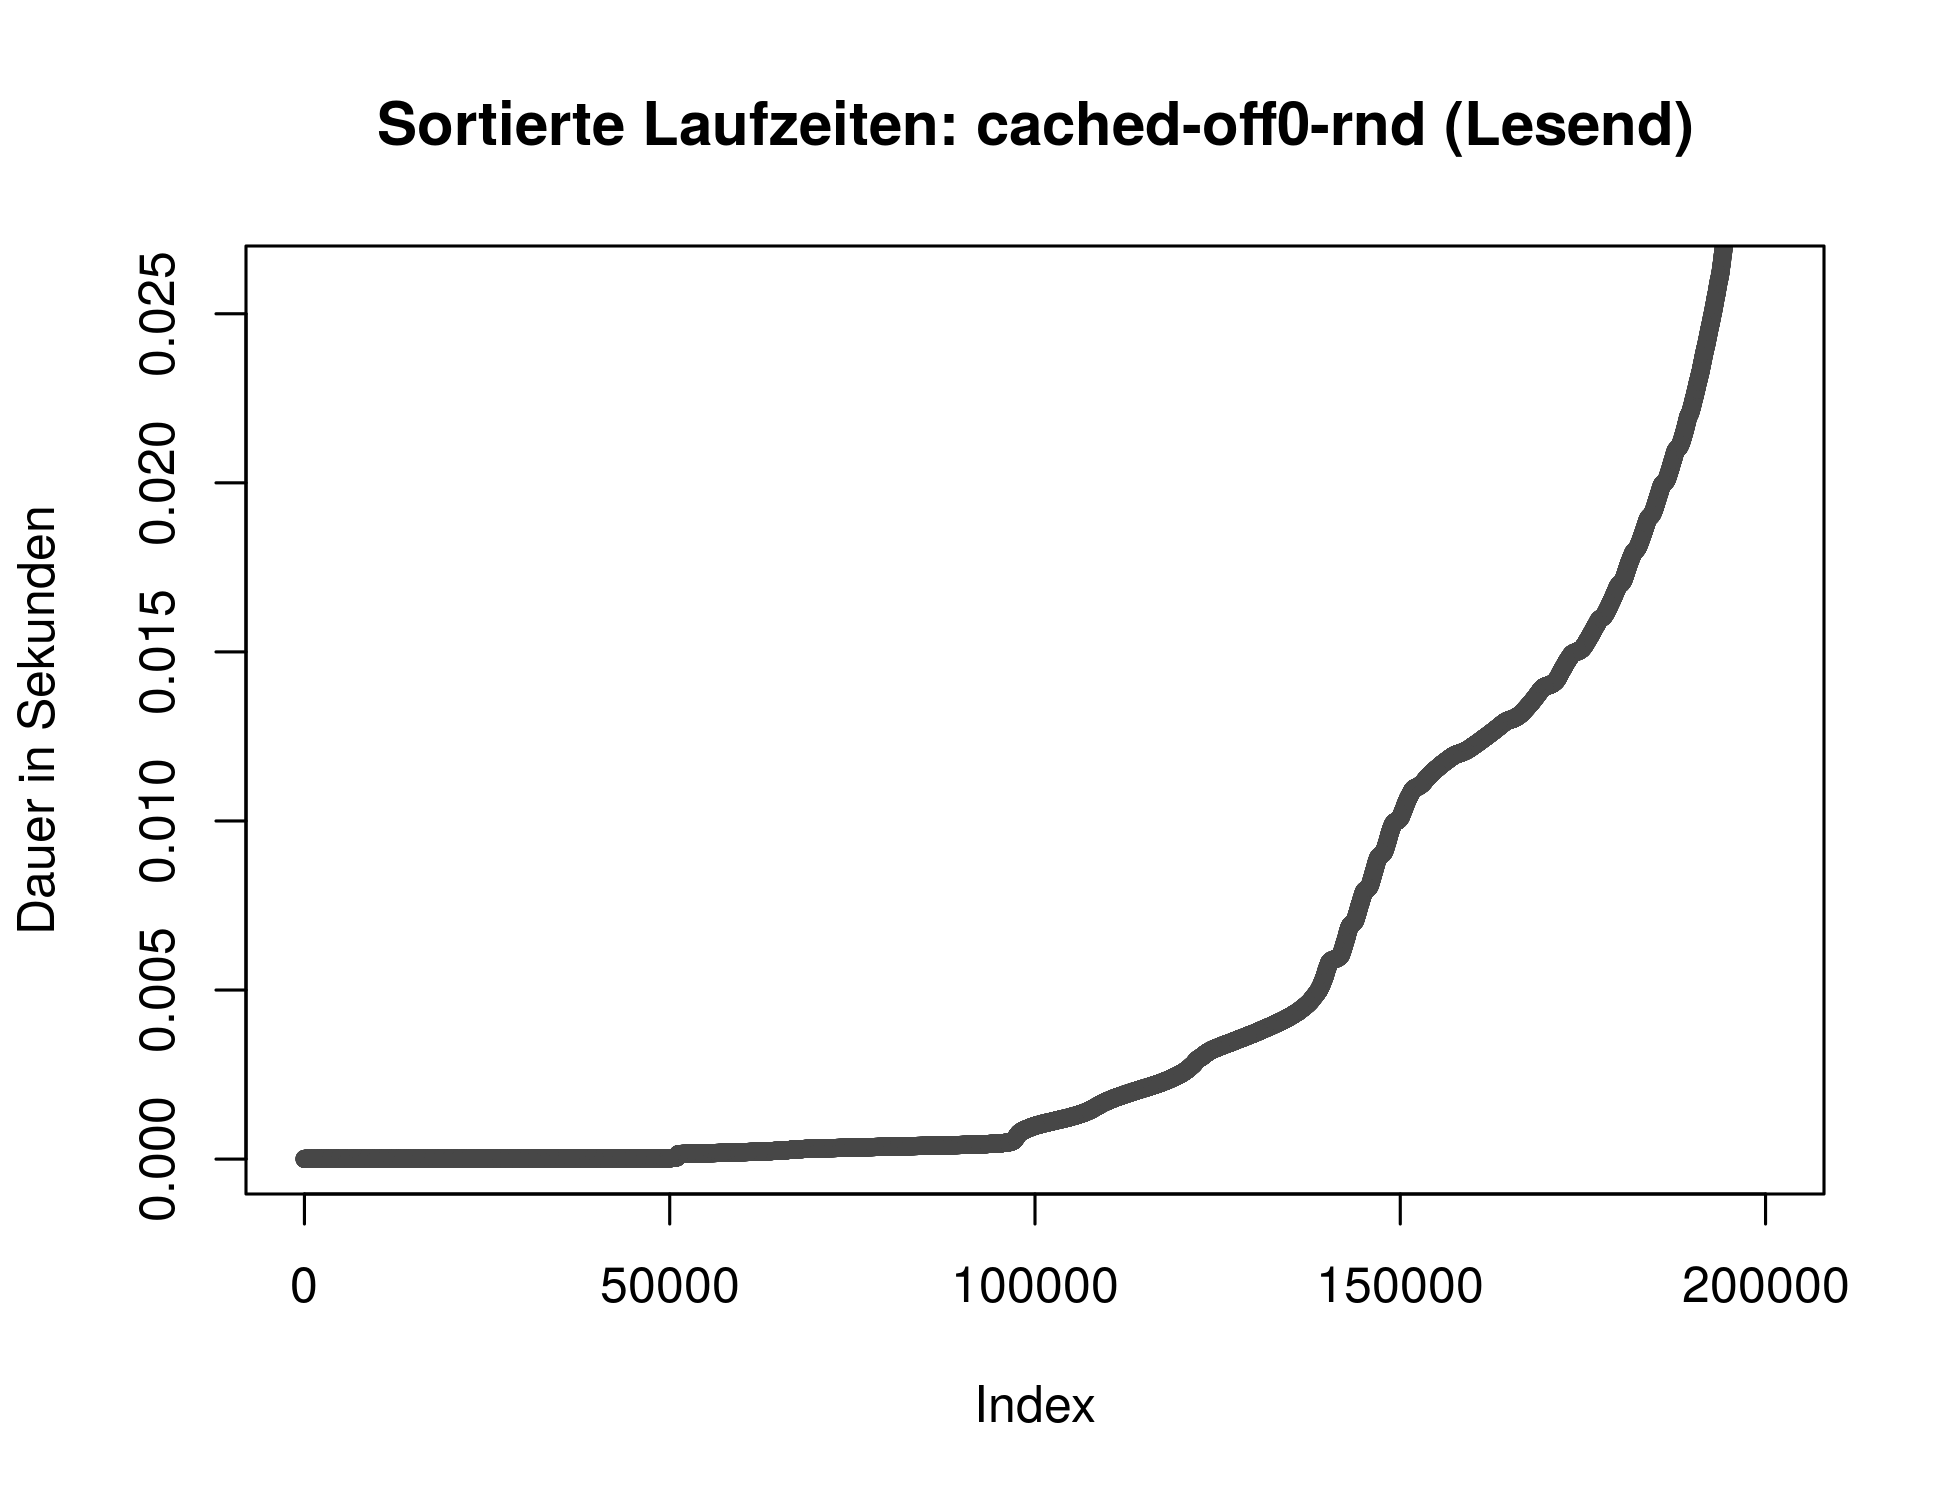
\includegraphics[width=.43\textwidth]{Bilder/Plots/exploration/plot_DurationSorted_read_rnd_nolog.png}
	}			
	\caption{Messungen der Laufzeiten sortiert dargestellt ohne Logarithmus}
	\label{Laufzeiten_Sortiert_nolog}
\end{figure} 

Als Ausreißer werden für alle \textbf{Attribut-Sets} die Messungen mit den $10\%$ kürzesten und längsten Laufzeiten behandelt. Die Verteilung der Ausreißer ist in \ref{fig:ausreisser} erkennen.\\
Am Verhalten der Ausreißer lässt sich gut unterscheiden, ob es sich um den sequentiellen oder den randomisierten Datensatz handelt. Bei cached-off0-seq befinden sich die Ausreißer gerade an den oberen und unteren Enden einer Ansammlung von Punkten. Da alle Punkte innerhalb der Ansammlung zu einem Attribut-Set gehören muss sich gerade dieses Bild ergeben. Dagegen sind die roten Punkte bei cached-off0-rnd unregelmäßiger verteilt. Da die Ausreißer als zweites in den Graphen gezeichnet wurden, überdecken sie die grauen und erscheinen daher präsenter. (\textbf{Sind die Ausreißer hier eher ein Zeichen dafür, dass das System in den Häufungspunkten von Ausreißern besonders schnell oder langsam  agiert hat, oder ist dies durch die Art des Benchmarks bedingt}?)

\begin{figure}
	\subfloat{
		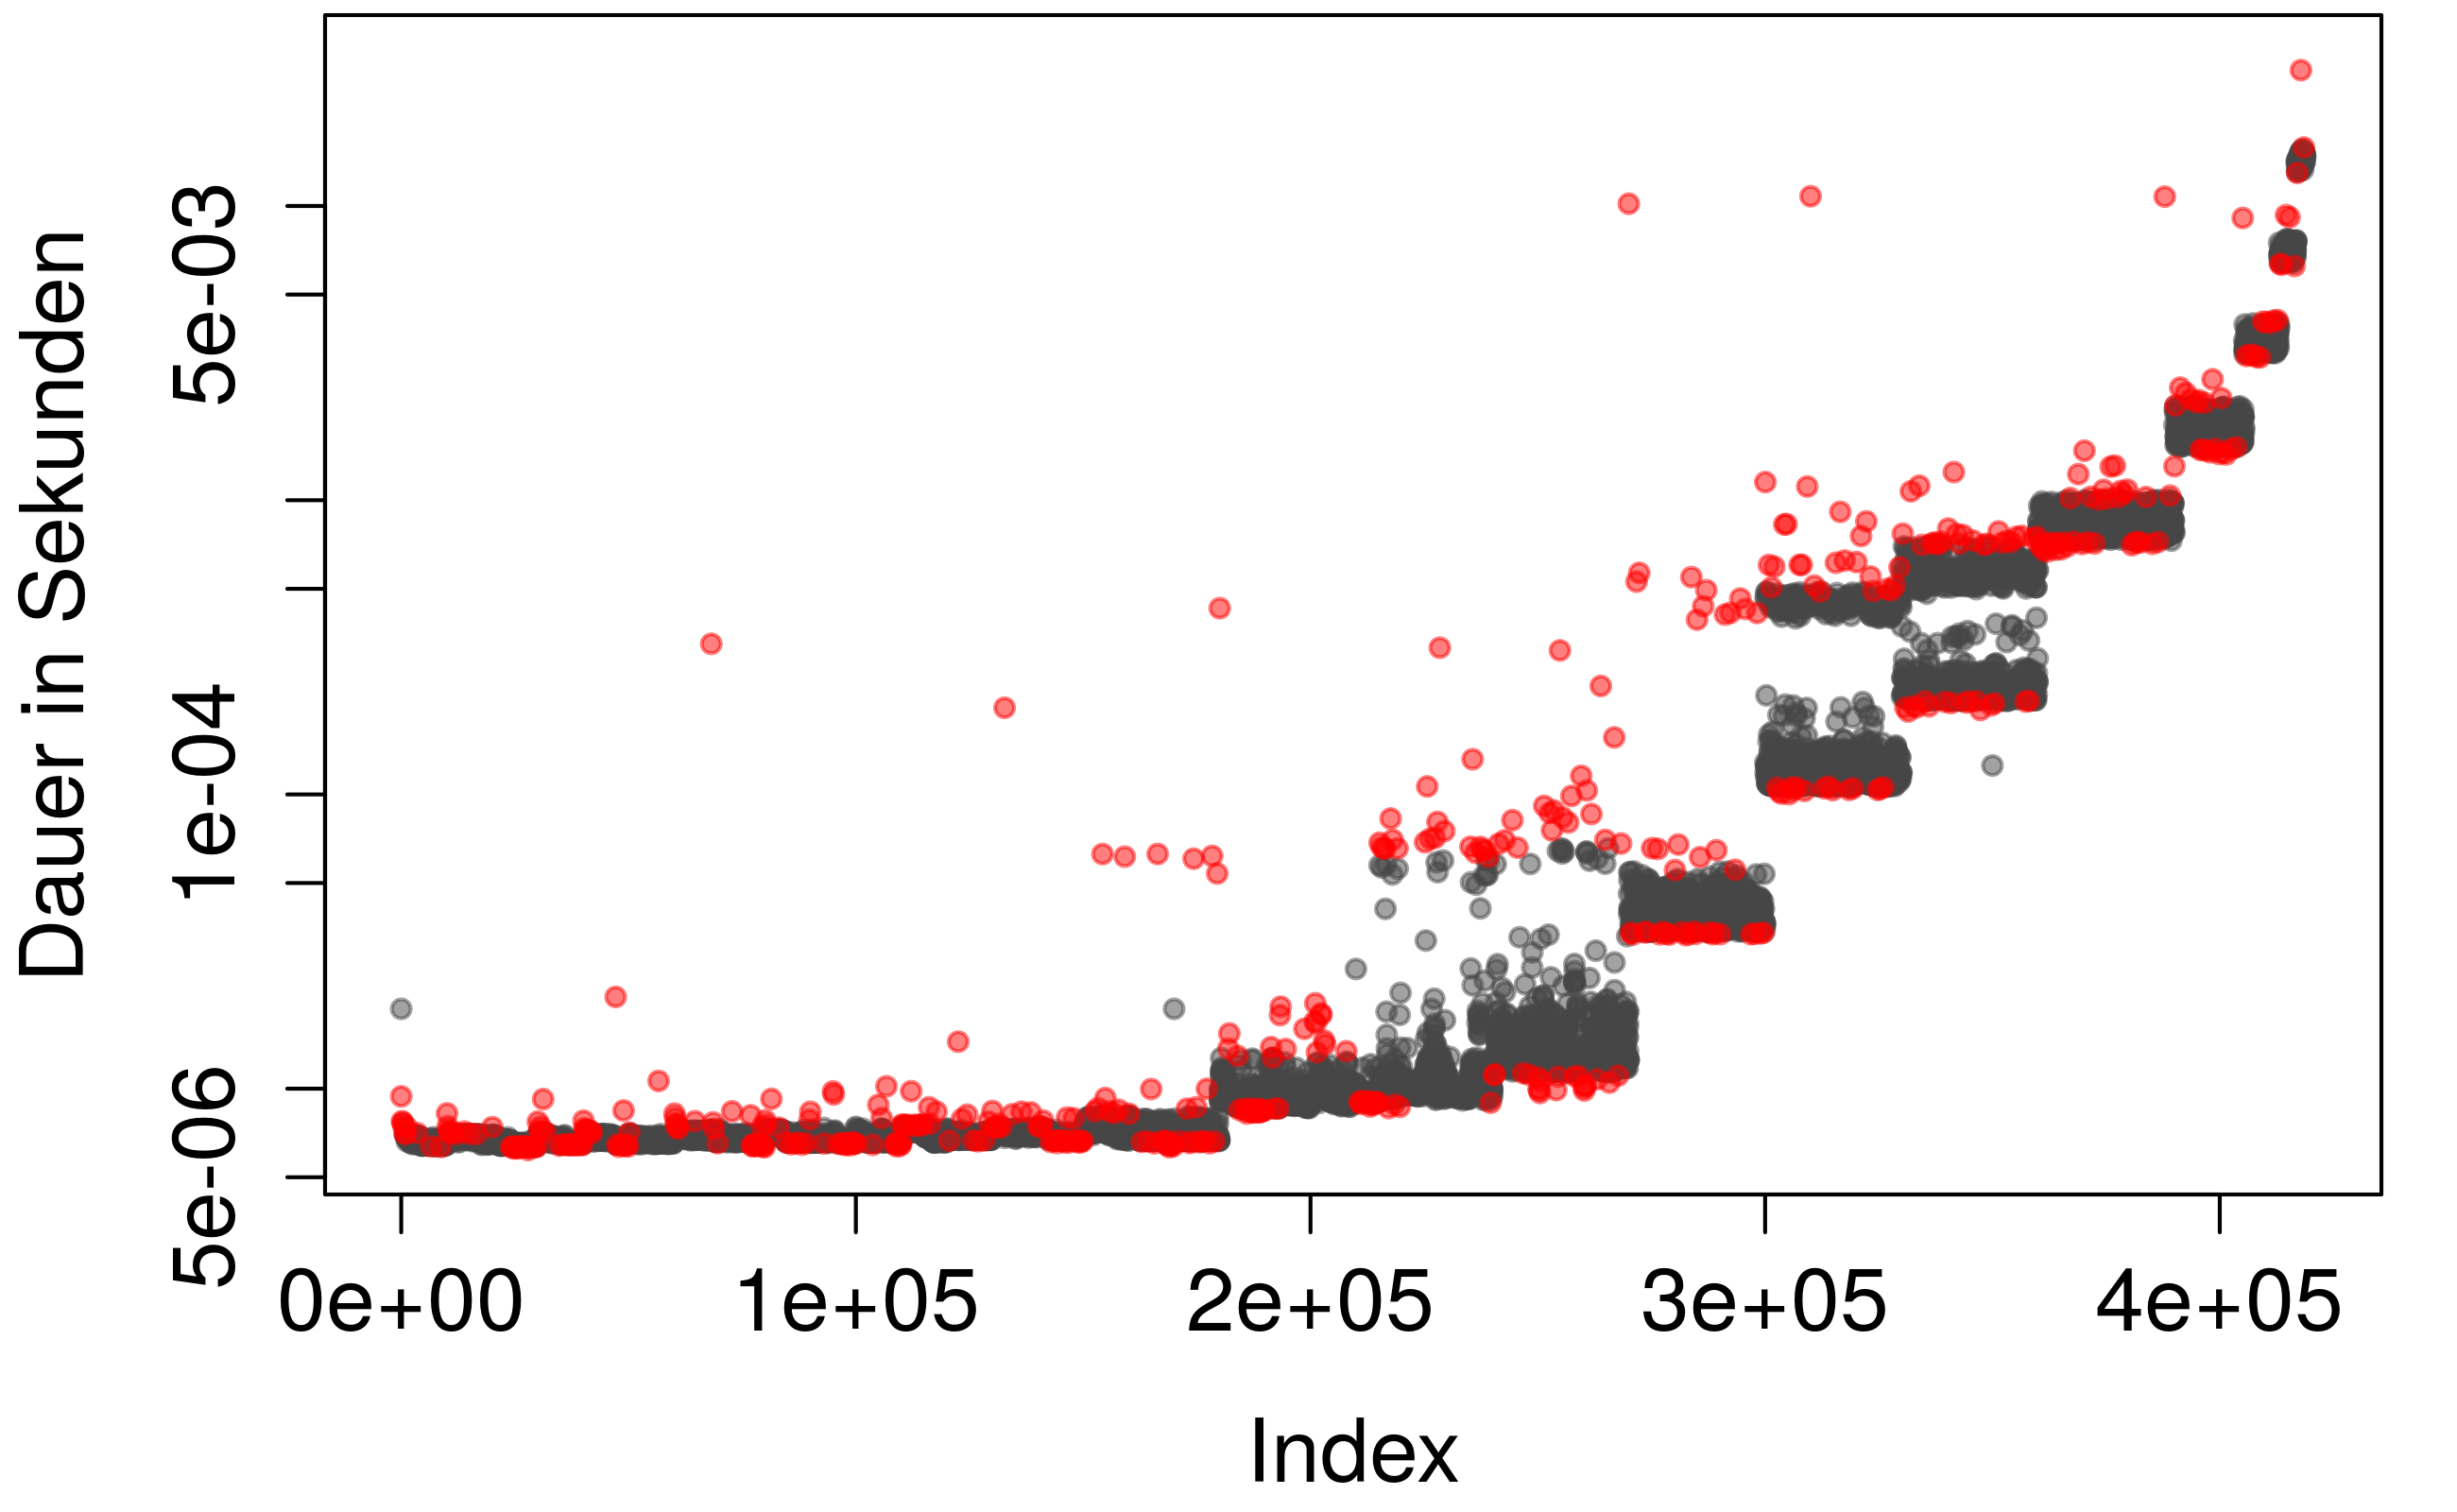
\includegraphics[width=.43\textwidth]{Bilder/Plots/exploration/plot_outlier_read_seq.png}
	}
	\hfill
	\subfloat{
		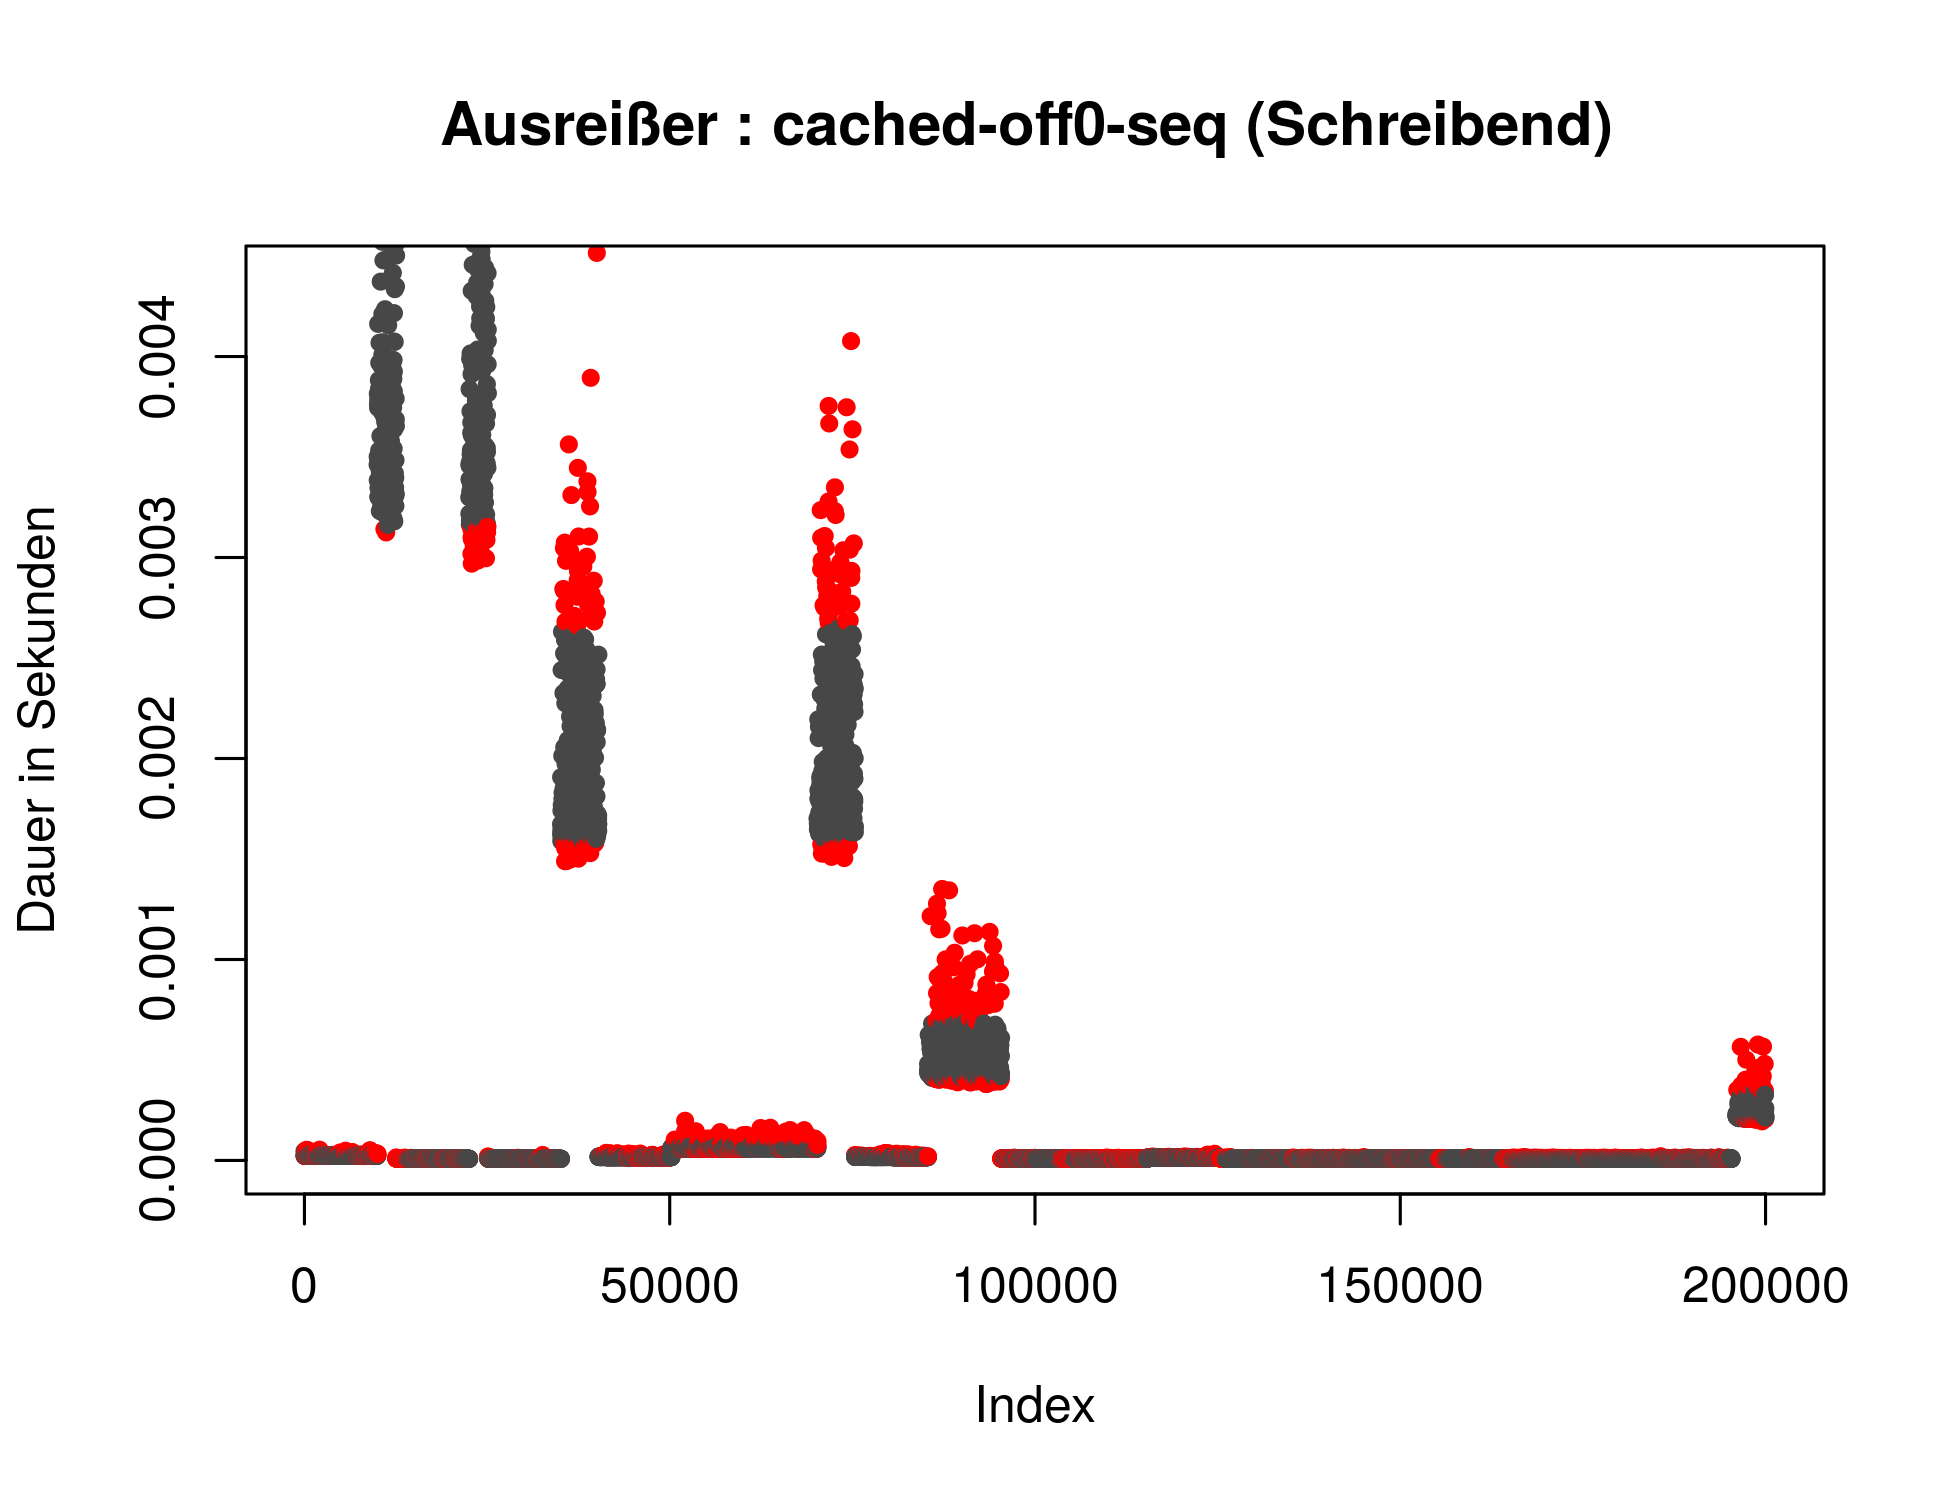
\includegraphics[width=.43\textwidth]{Bilder/Plots/exploration/plot_outlier_write_seq.png}
	}\\
	\subfloat{
		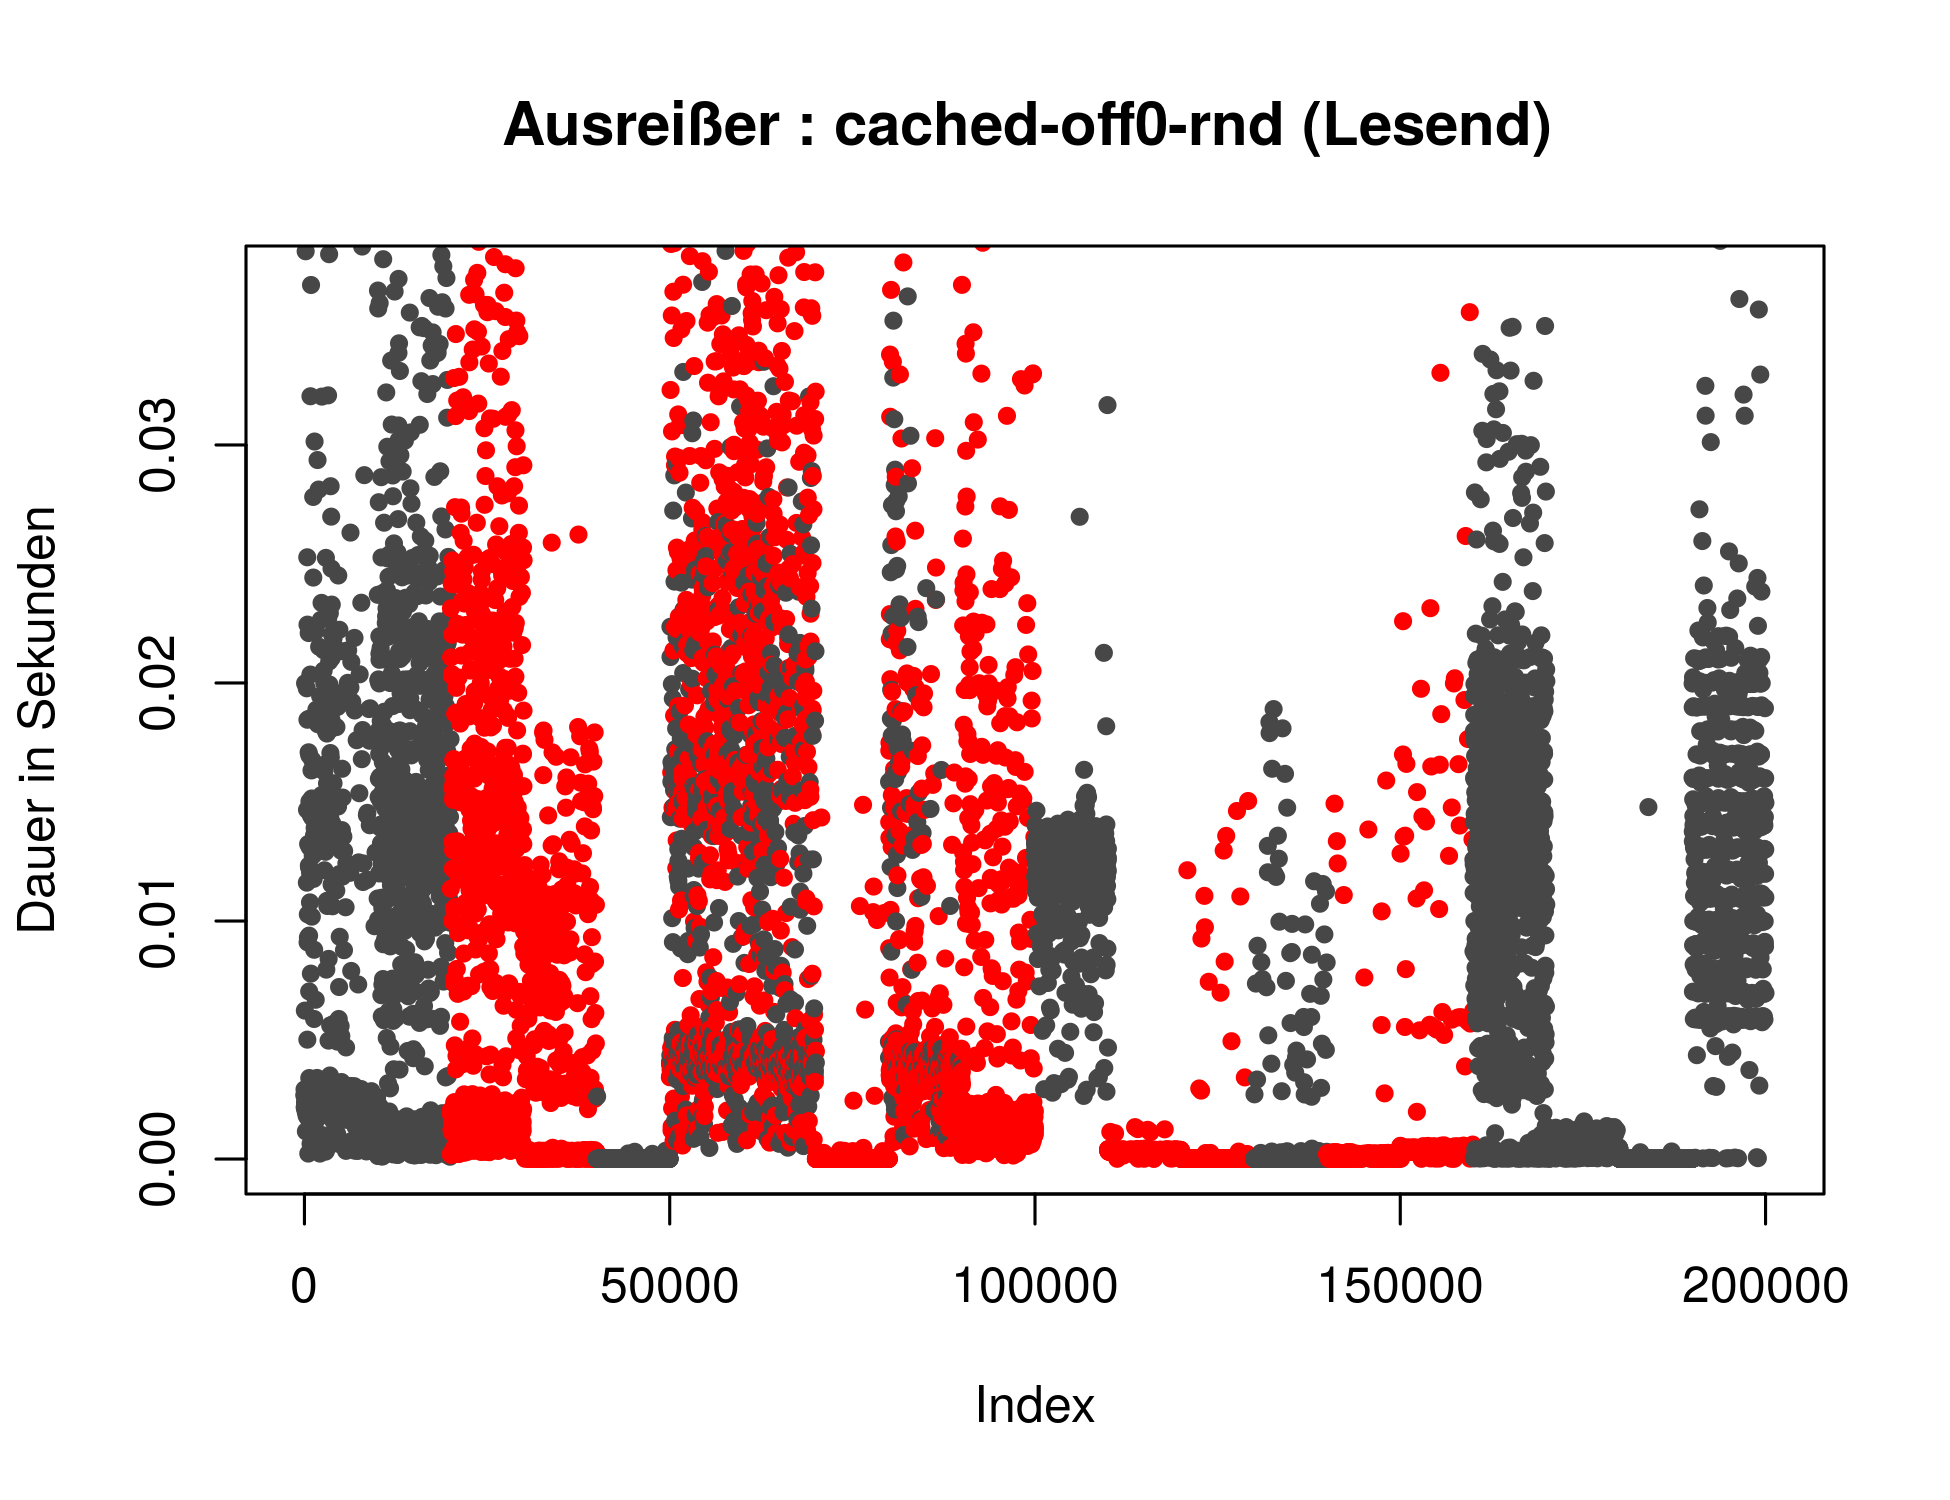
\includegraphics[width=.43\textwidth]{Bilder/Plots/exploration/plot_outlier_read_rnd.png}
	}
	\hfill
	\subfloat{
		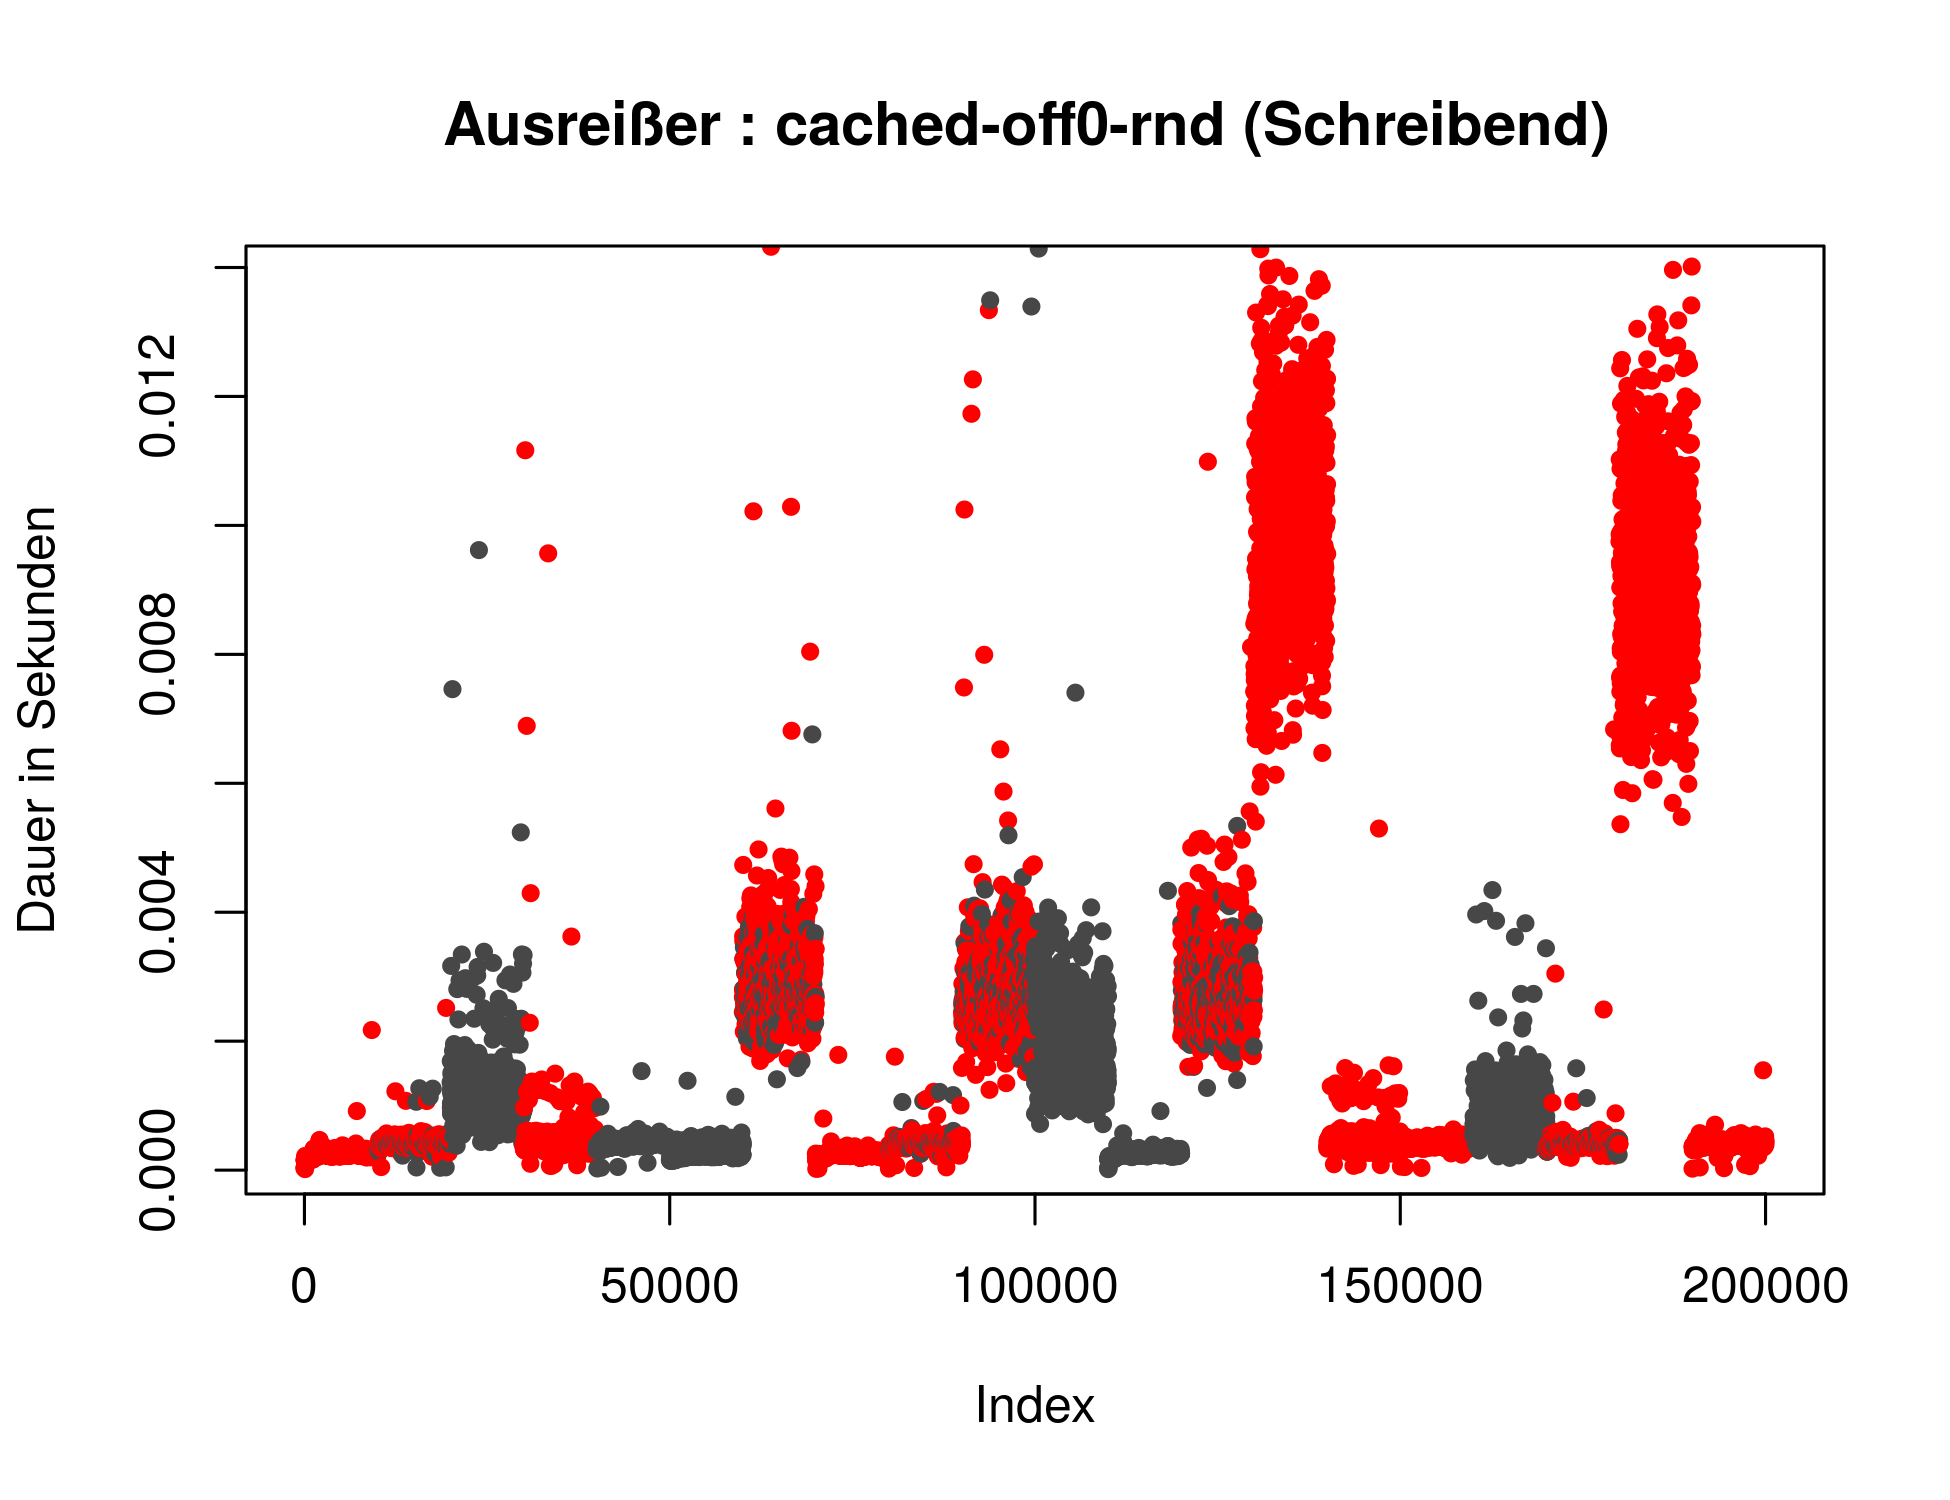
\includegraphics[width=.43\textwidth]{Bilder/Plots/exploration/plot_outlier_write_rnd.png}
	}		
	\caption{Ausreißer sind in rot dargstellt, sie überdecken die grauen Punkte}
	\label{fig:ausreisser}
\end{figure} 

Bei der Betrachtung der Metainformationen wurde festgestellt, dass die Zugriffsgröße sehr stark mit der Laufzeit eines Messpunktes korreliert. Um eine Vorstellung davon zu entwickeln, wie diese beiden Größen miteinander zusammenhängen, habe ich die Messdaten nach der Zugriffsgröße sortiert und ihre Laufzeit aufgetragen. \ref{fig:Zugriffsgroesse_Sortiert} \\
Die Korrelation der beiden Größen ist deutlich erkennbar, die Laufzeiten nehmen im Mittel zu. Doch es ist auch zu erkennen, insbesondere bei cached-off0-rnd-R, dass die Laufzeiten aufgrund der Streuung von weiteren Faktoren abhängen müssen. Die Verteilung der Messpunkte einer Zugriffsgröße in zwei bis drei deutlich zu unterscheidende Gruppen deutete darauf hin, dass Messungen innerhalb einer vom E/A-System Gruppe ähnlich behandelt wurden.

\begin{figure}
	\subfloat[Von links nach rechts in KB: 1, 4, 16, 256, 1024, 16384, 65536, 262144, 524288, 1048576, 2097152, 4194304, 8388608, 16777216]{
		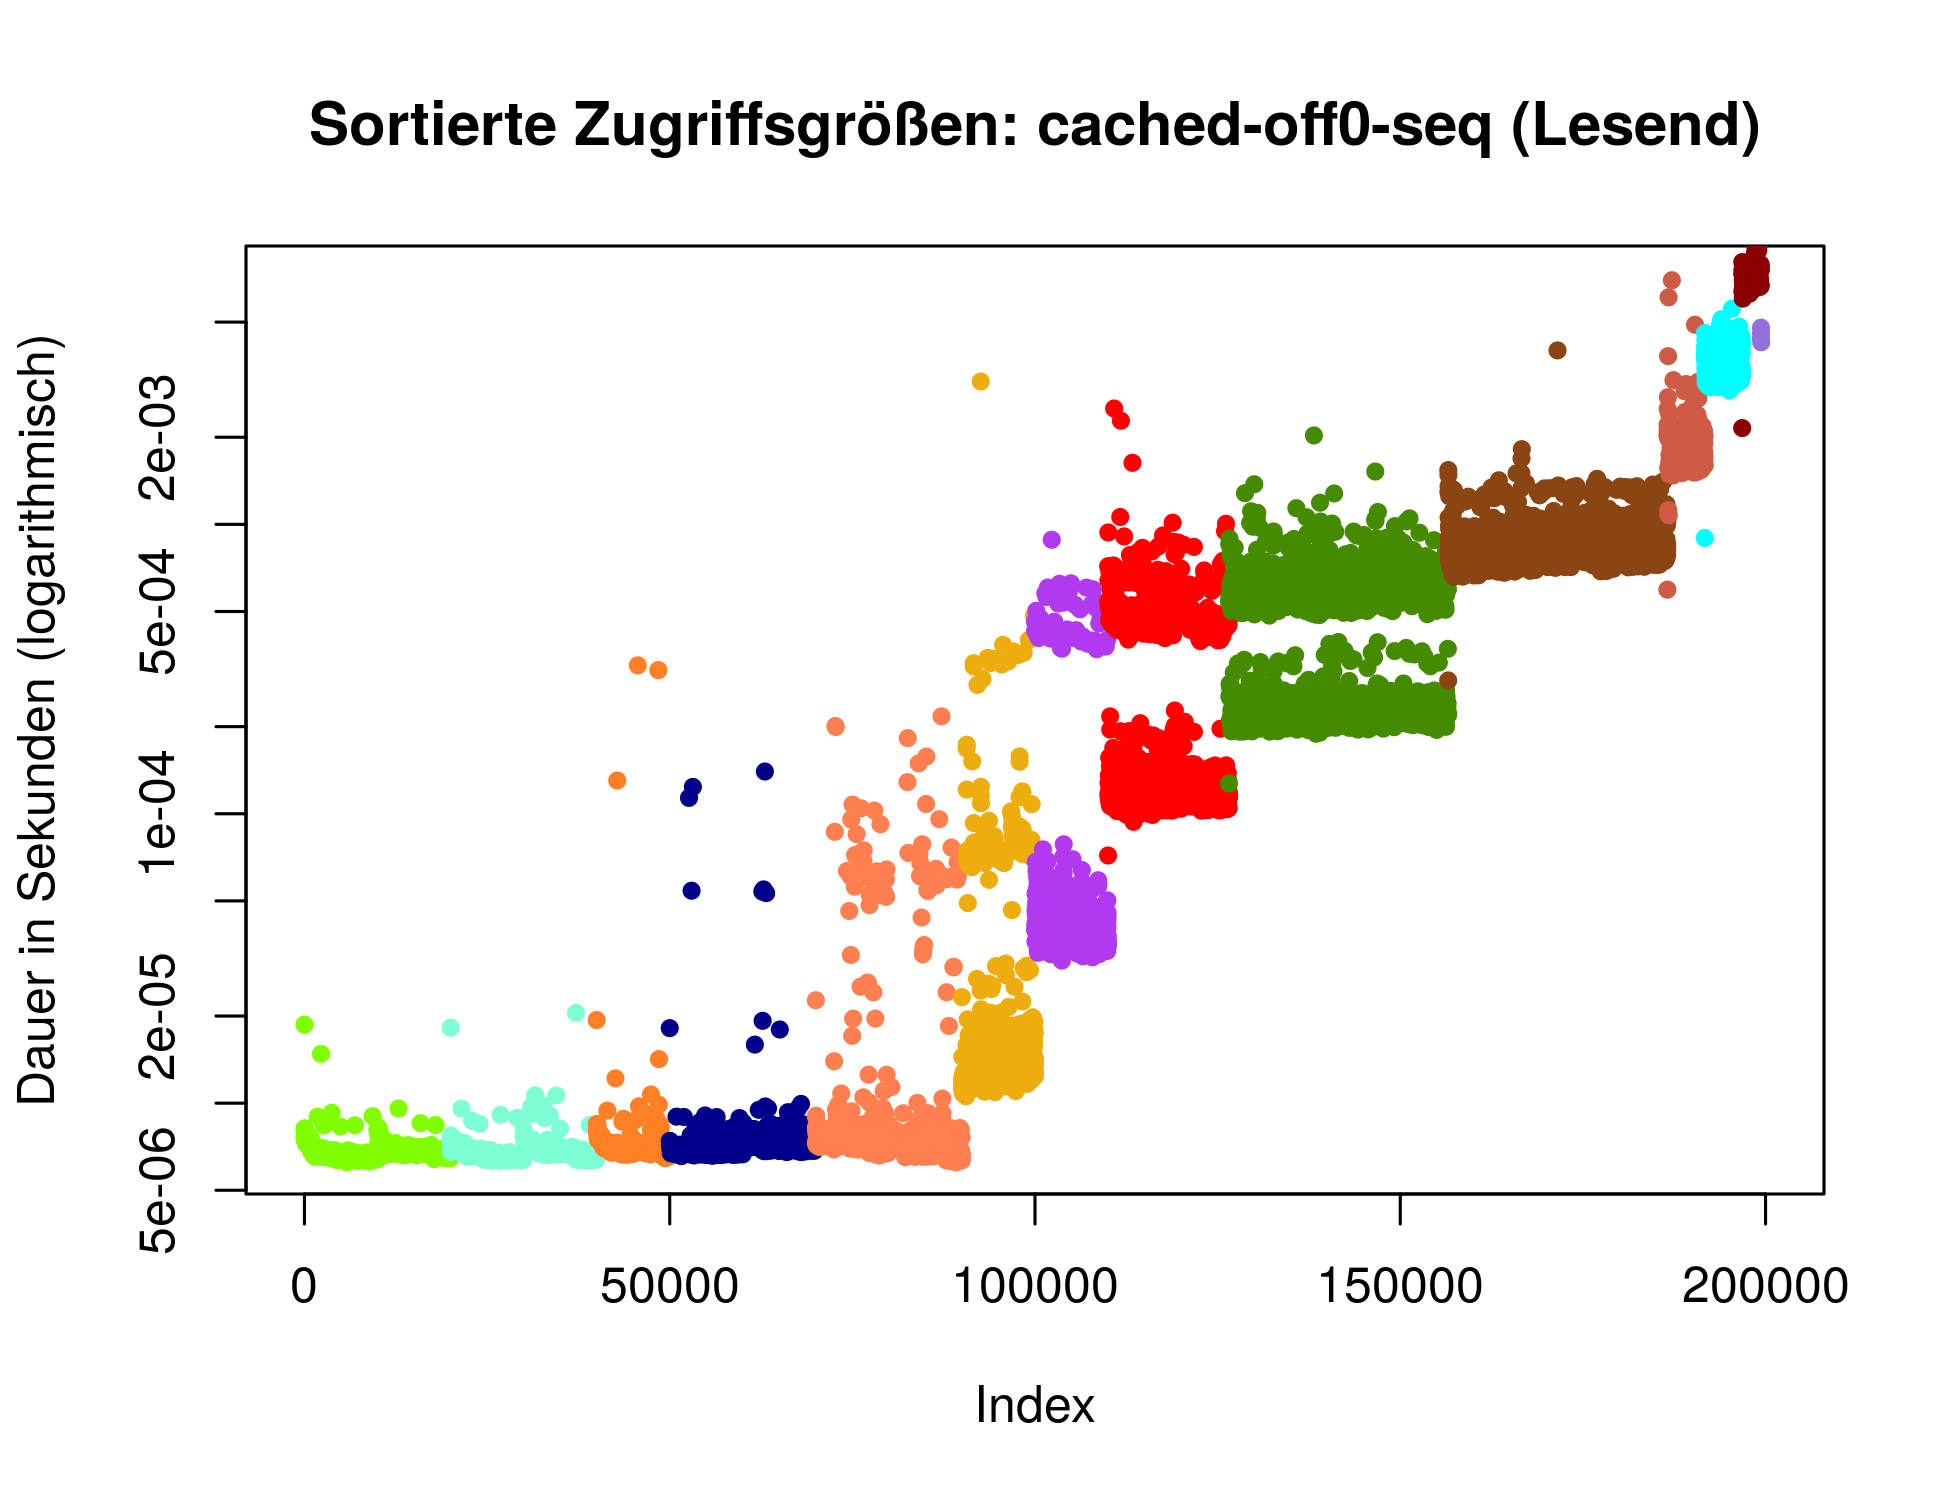
\includegraphics[width=.5\textwidth]{Bilder/Plots/exploration/plot_SizeSorted_read_seq.png}
	}
	\hfill
	\subfloat[Von links nach rechts in KB: 1, 4, 16, 64, 256, 1024, 4096, 8192, 16384, 65536, 262144, 524288, 2097152, 4194304, 16777216]{
		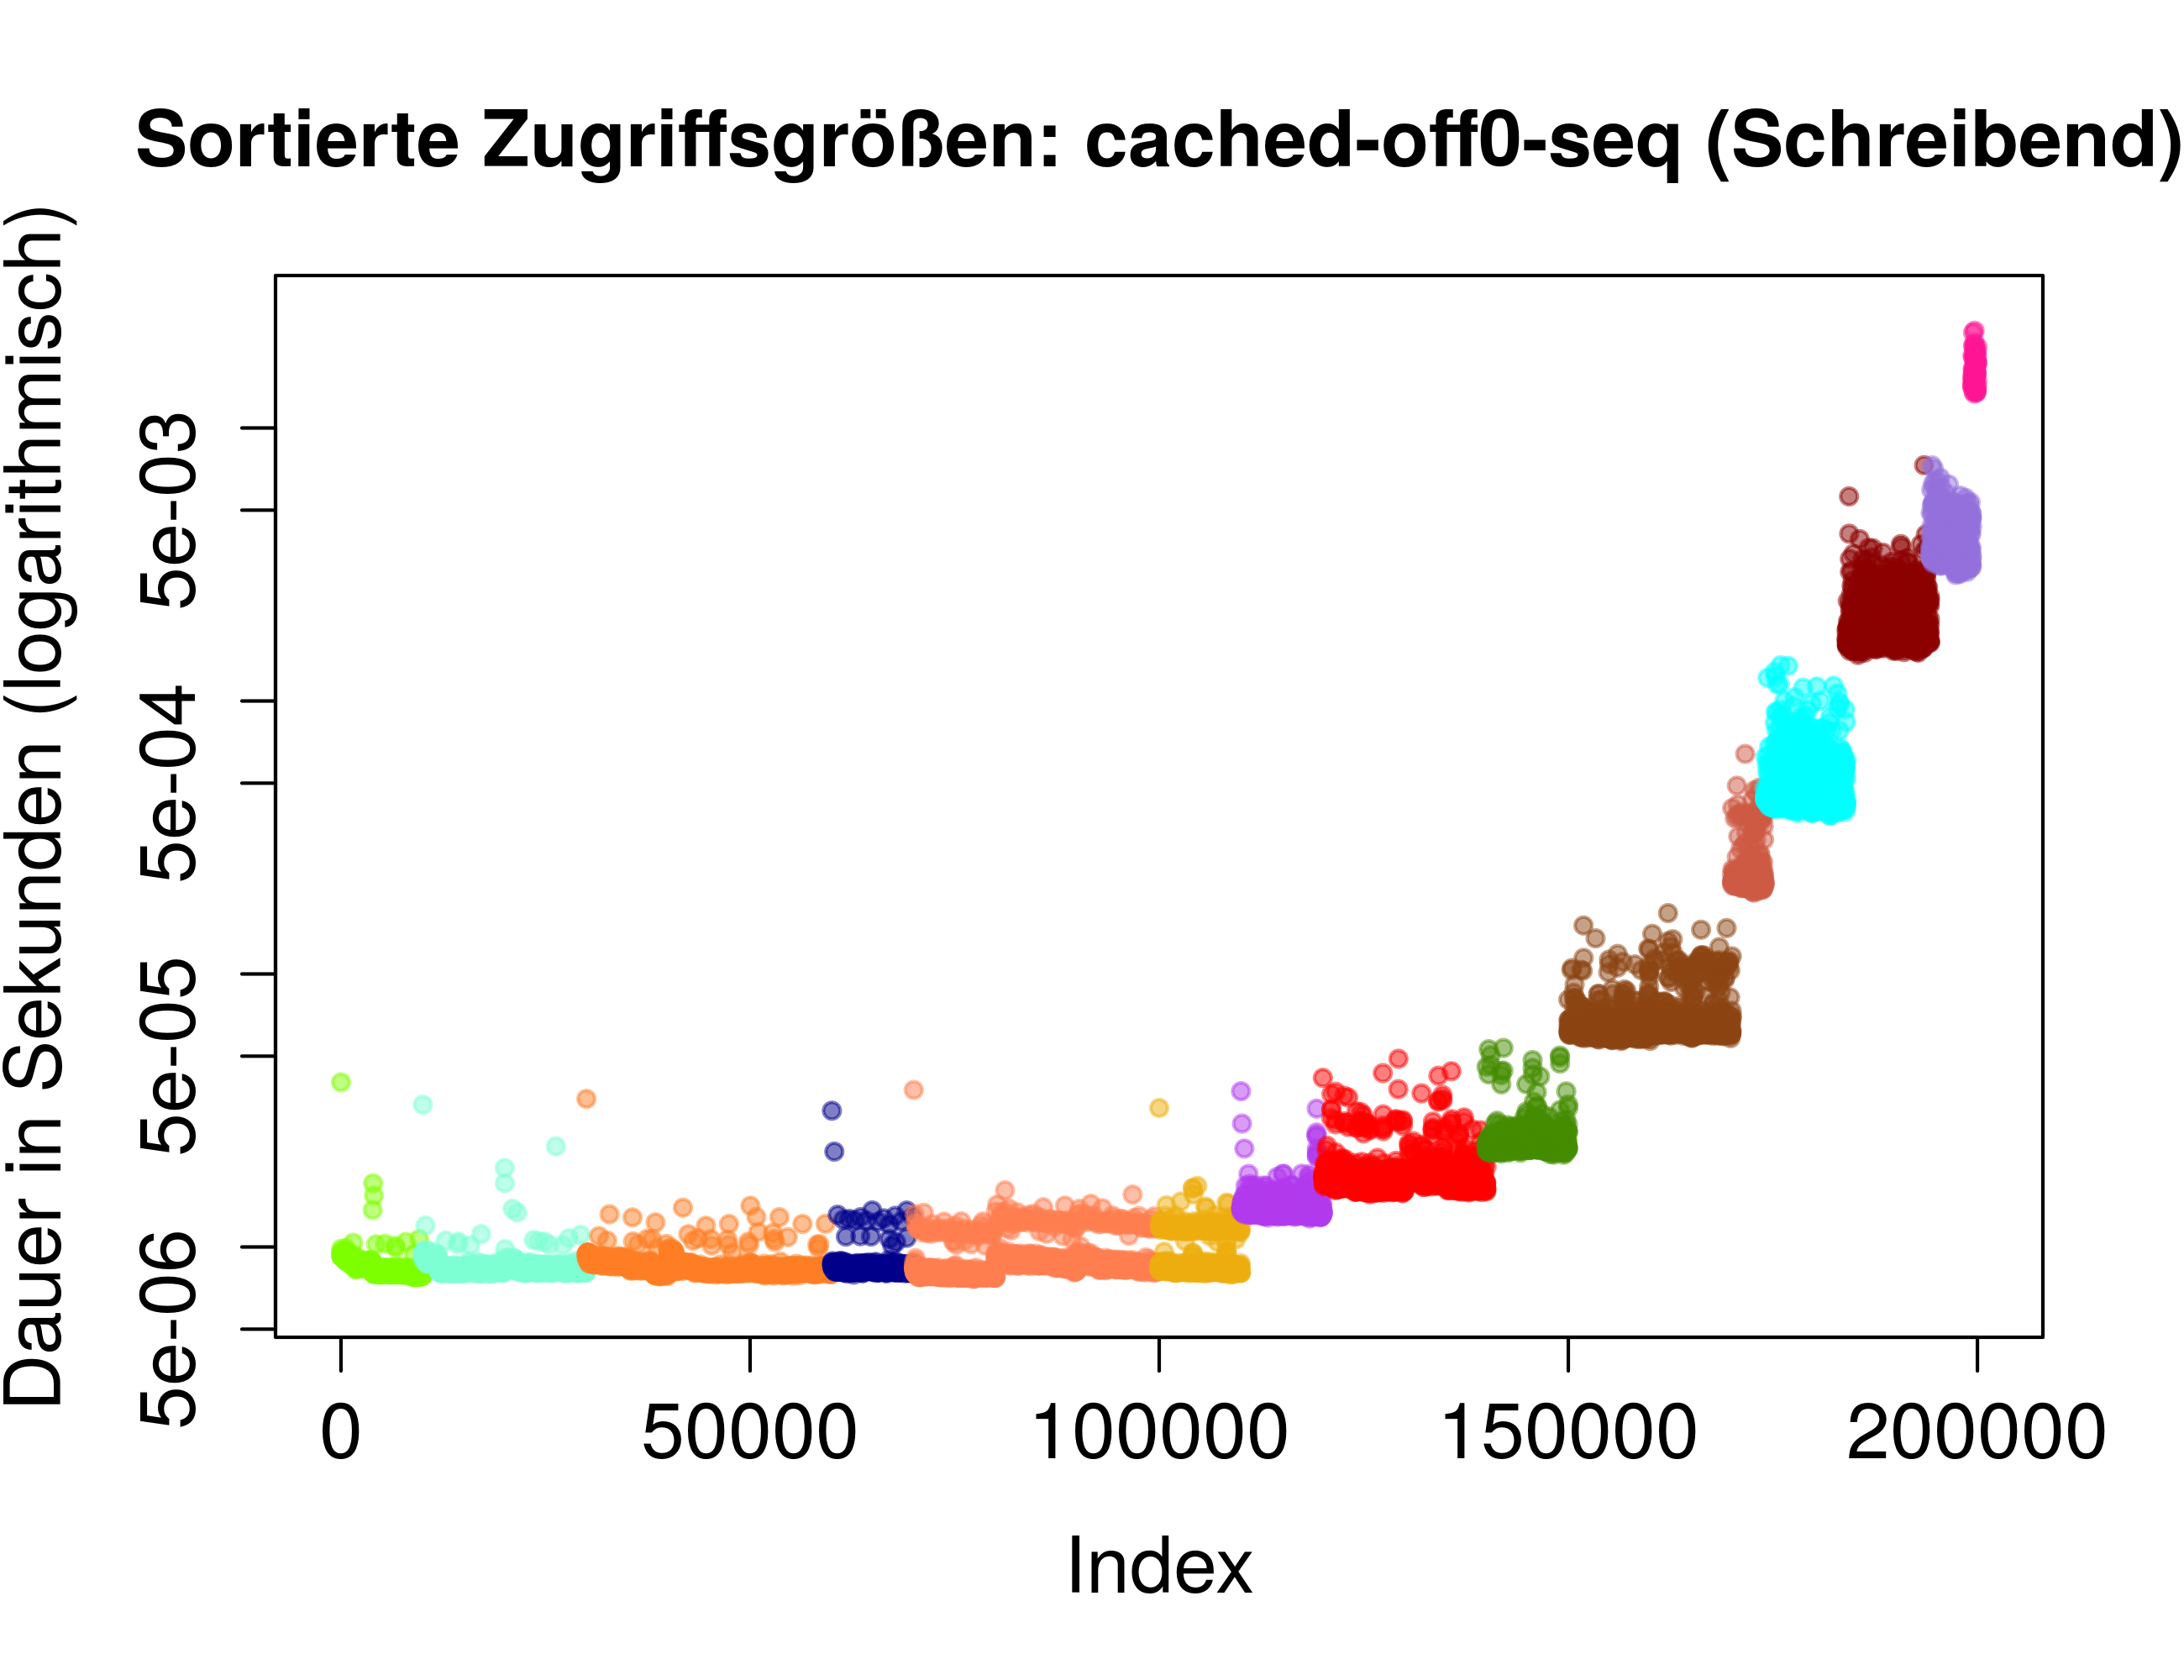
\includegraphics[width=.5\textwidth]{Bilder/Plots/exploration/plot_SizeSorted_write_seq.png}
	}\\
	\subfloat[Von links nach rechts in KB: 1, 4, 16, 64, 256, 4096, 8192, 16384, 65536, 262144, 524288, 1048576, 2097152, 8388608]{
		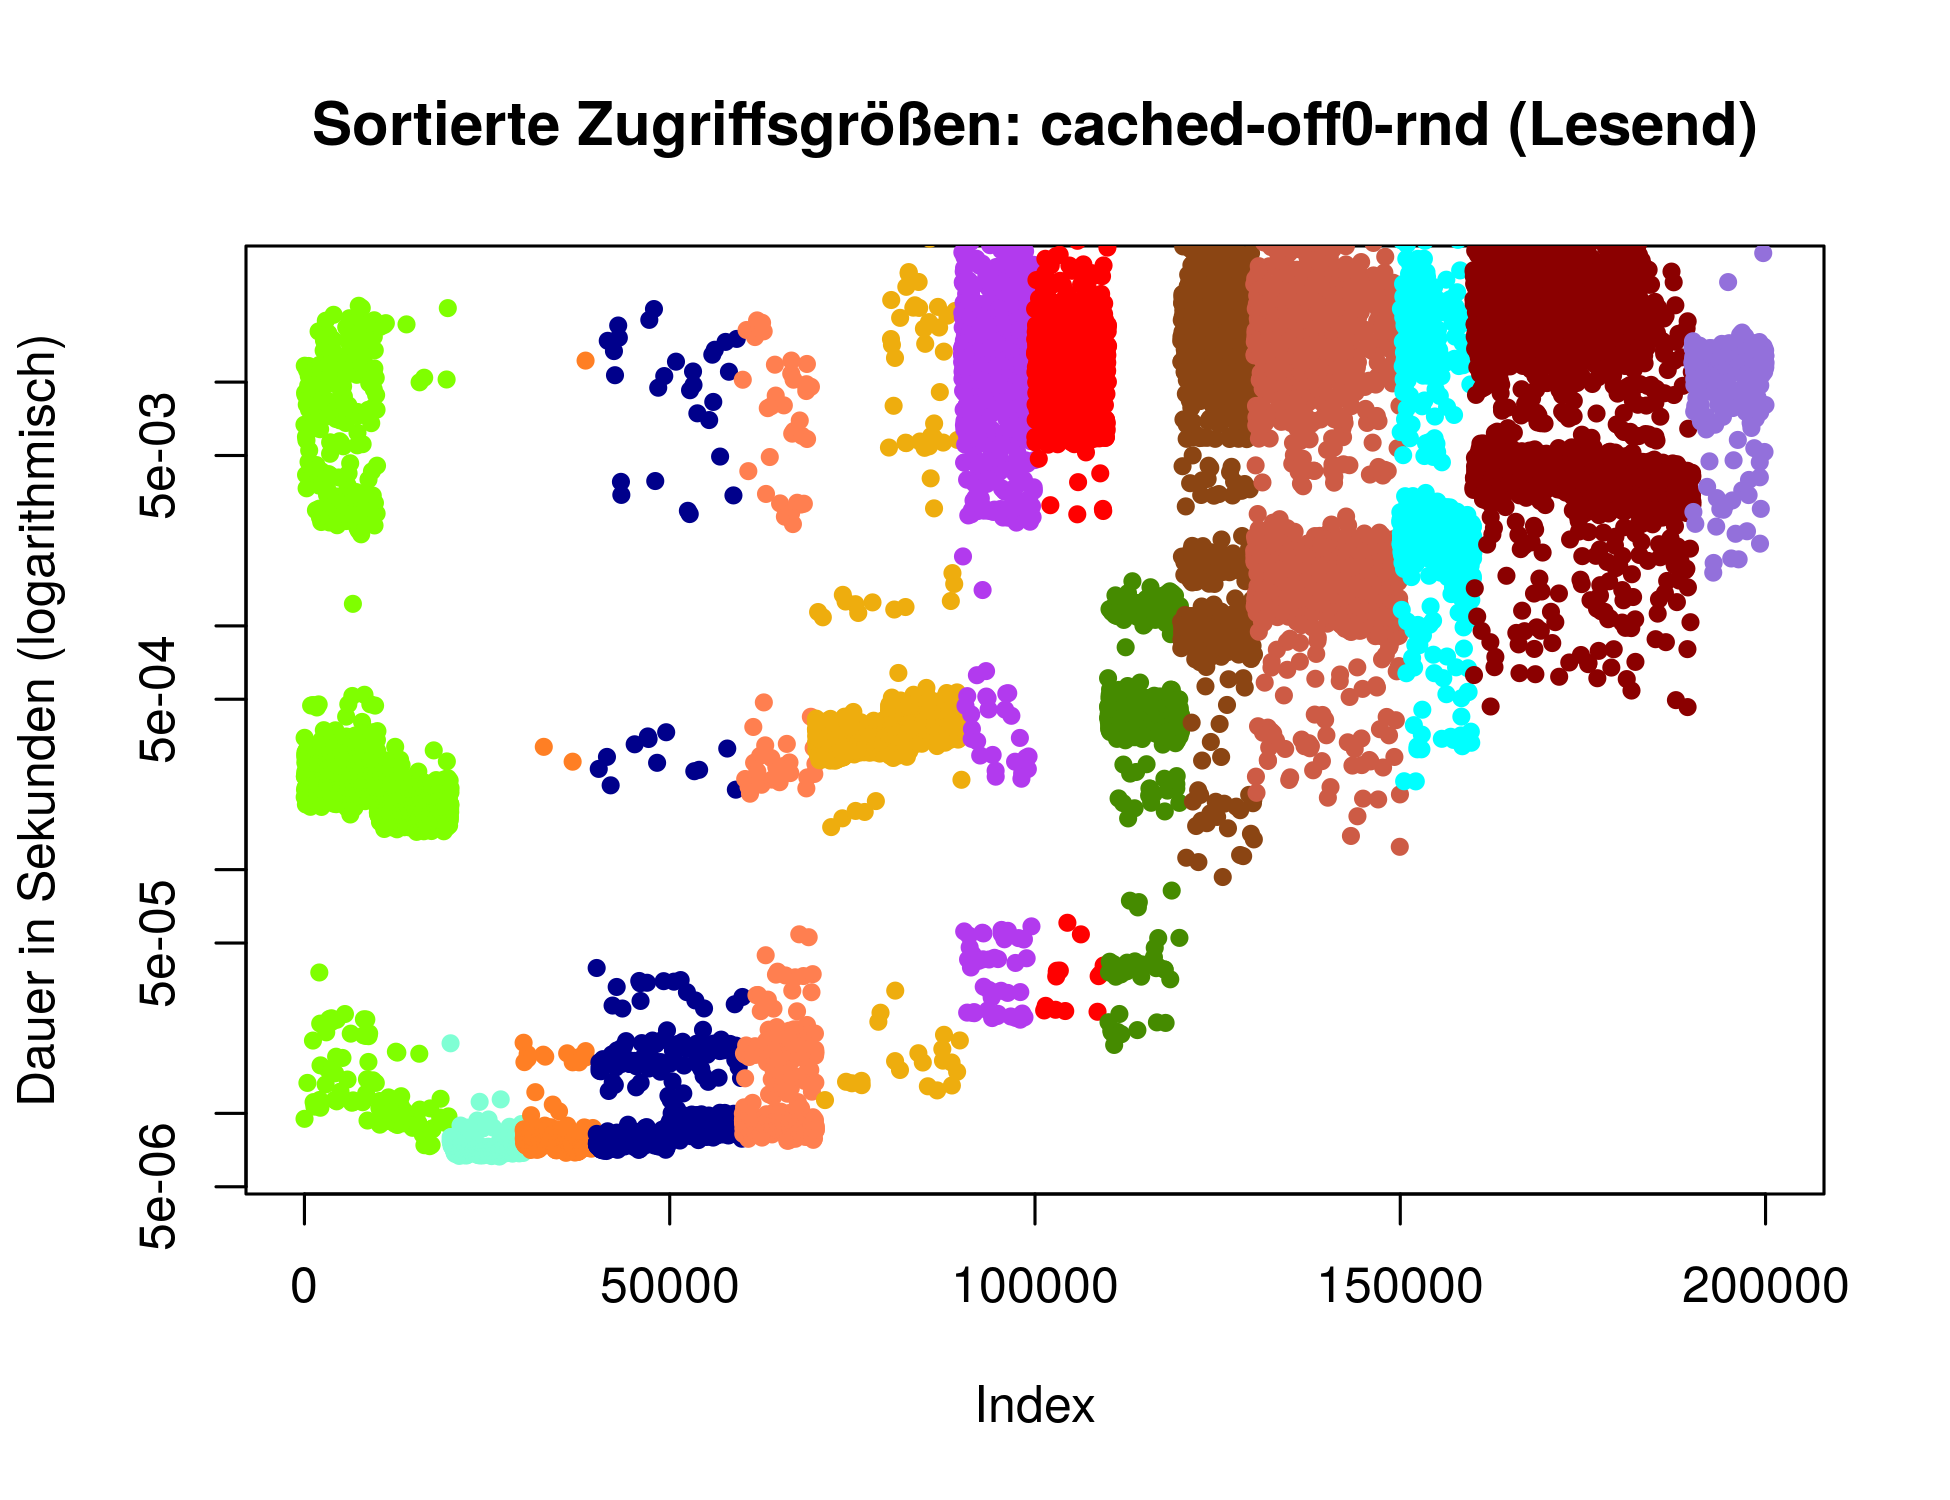
\includegraphics[width=.5\textwidth]{Bilder/Plots/exploration/plot_SizeSorted_read_rnd.png}
	}
	\hfill
	\subfloat[Von links nach rechts in KB: 1, 4, 1024, 4096, 8192, 16384, 65536, 262144, 524288, 1048576, 2097152, 8388608]{
		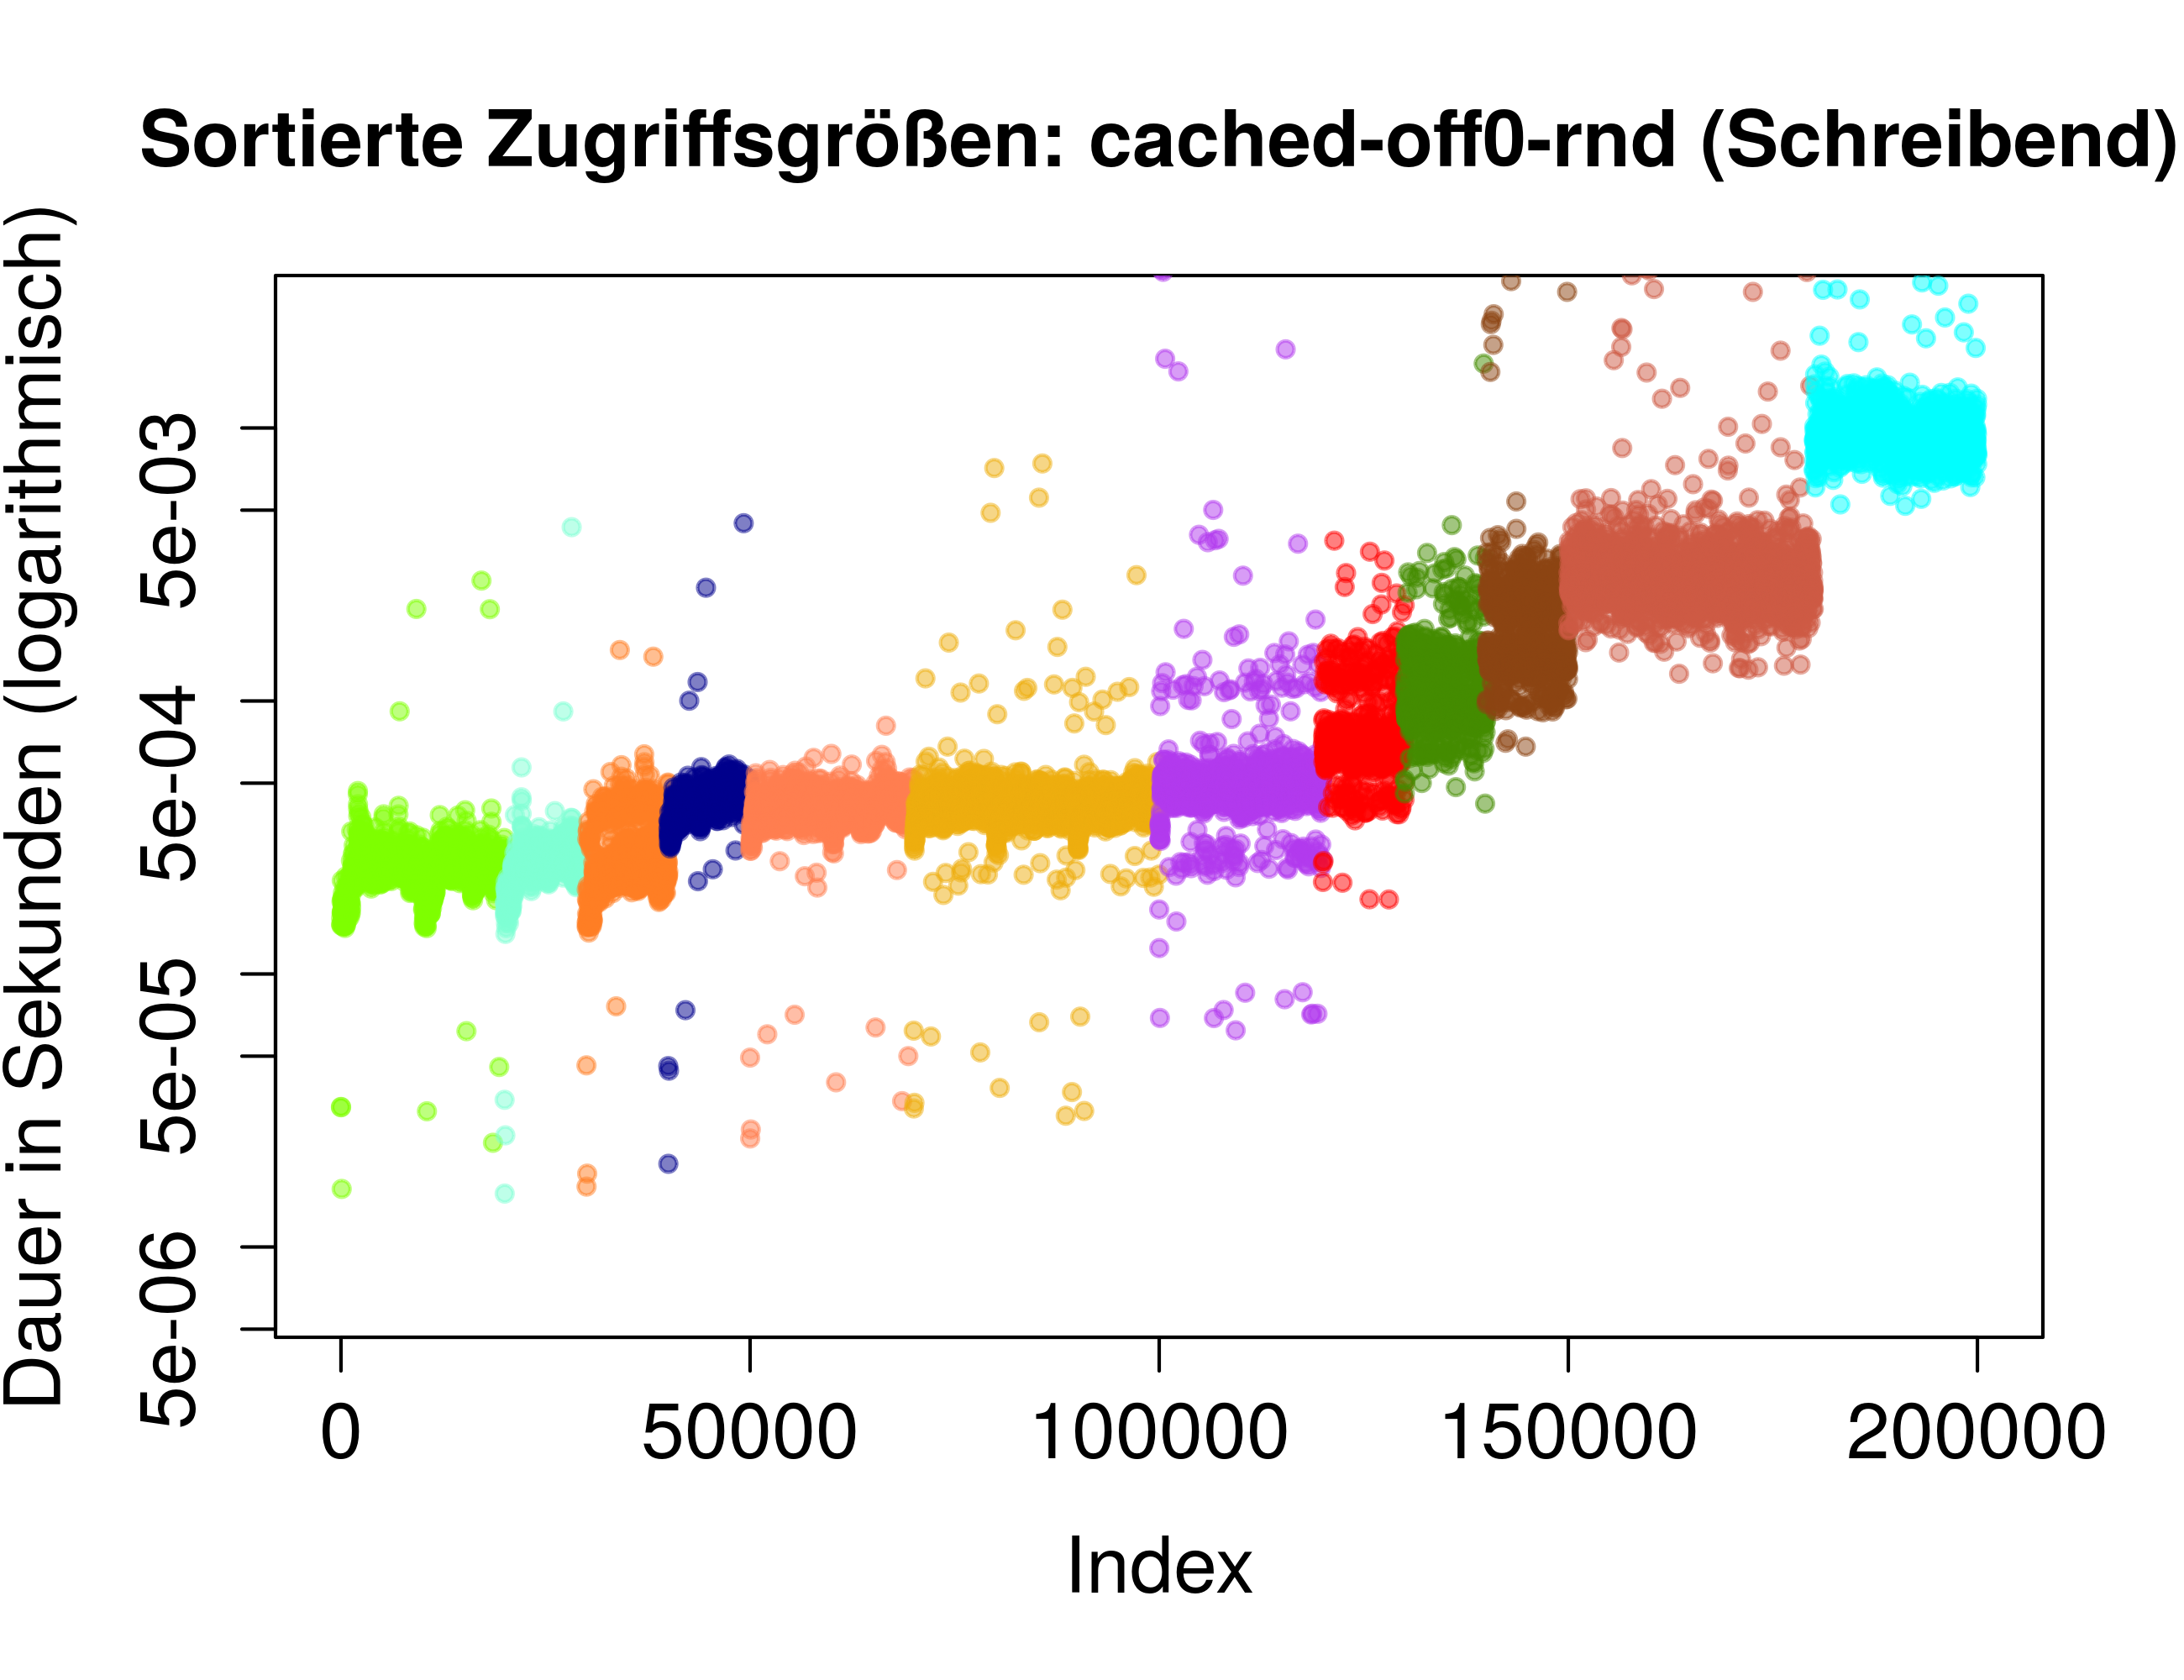
\includegraphics[width=.5\textwidth]{Bilder/Plots/exploration/plot_SizeSorted_write_rnd.png}
	}		
	\caption{Messungen der Laufzeiten nach Zugriffsgröße sortiert dargestellt (logarithmische Y-Achse)}
	\label{fig:Zugriffsgroesse_Sortiert}
\end{figure} 

Um die unterschiedlichen Laufzeiten innerhalb einer Zugriffsgröße zu untersuchen, habe ich für die Größen 1KB, 16384KB und 2097152KB (diese Zugriffsgrößen kommen in allen vier Datensätzen vor) alle Messungen betrachtet.

\begin{figure}
	\subfloat{
		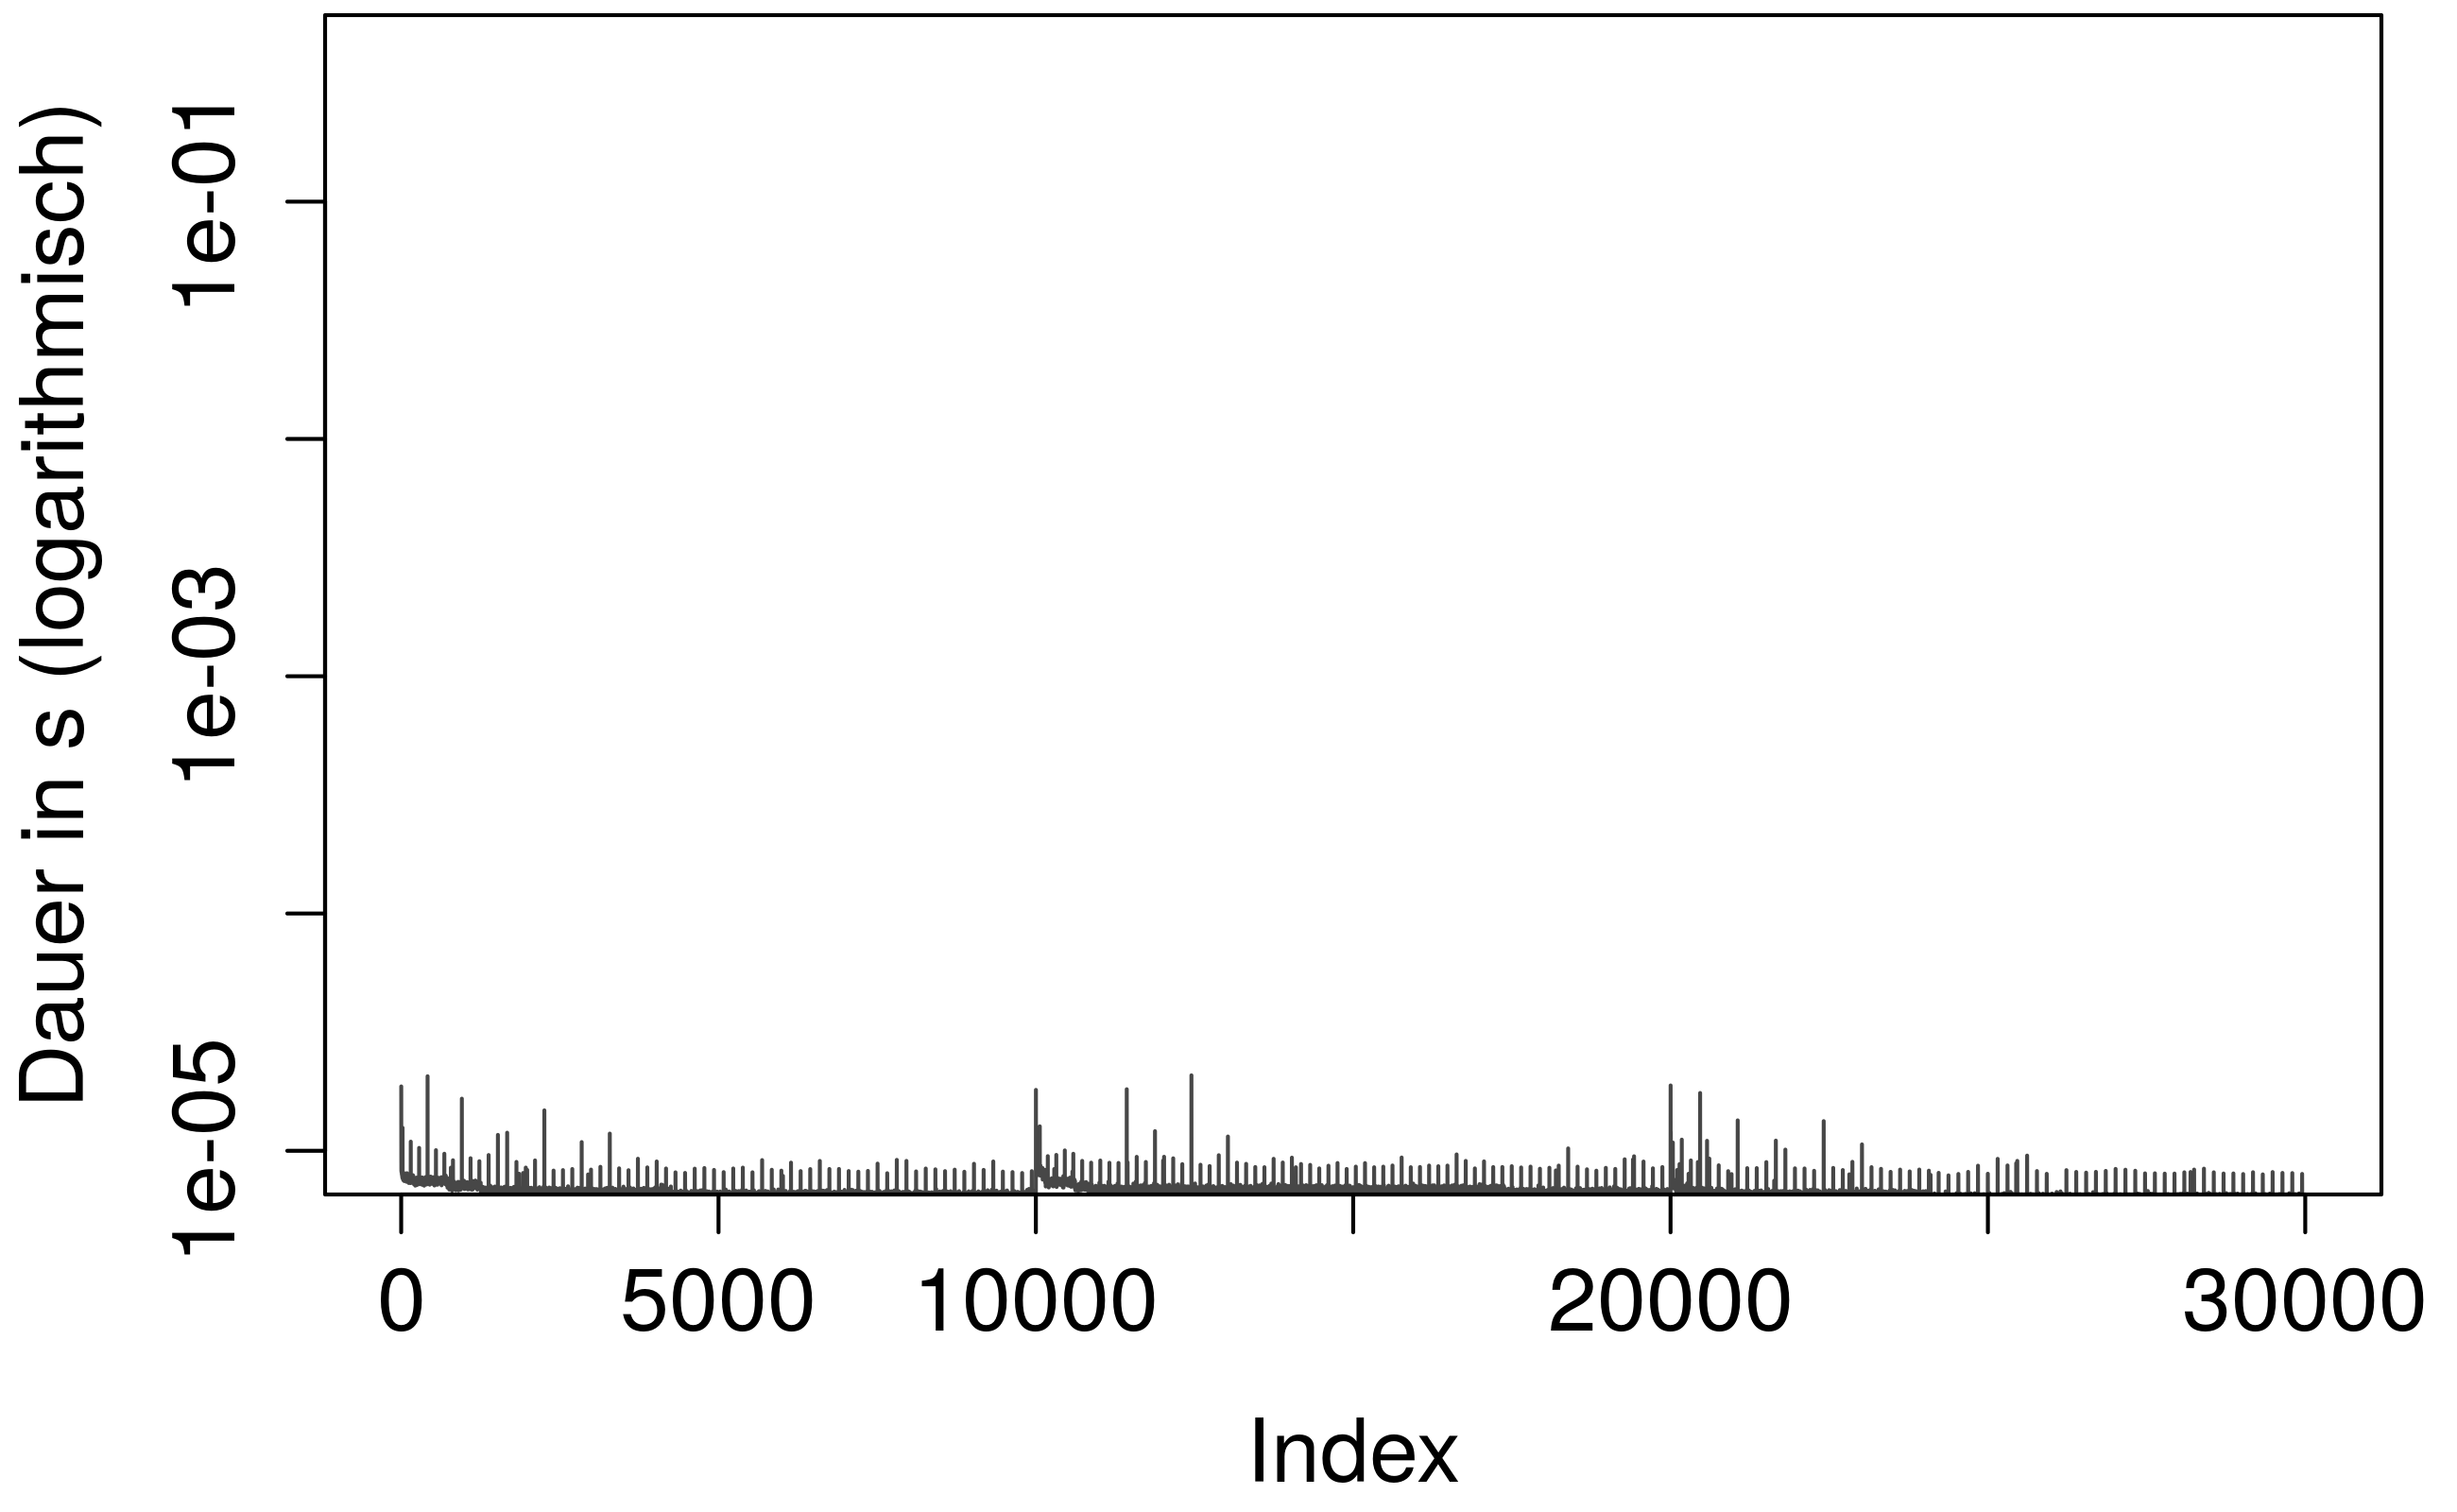
\includegraphics[width=.43\textwidth]{Bilder/Plots/exploration/plot_Size1_read_seq.png}
	}
	\hfill
	\subfloat{
		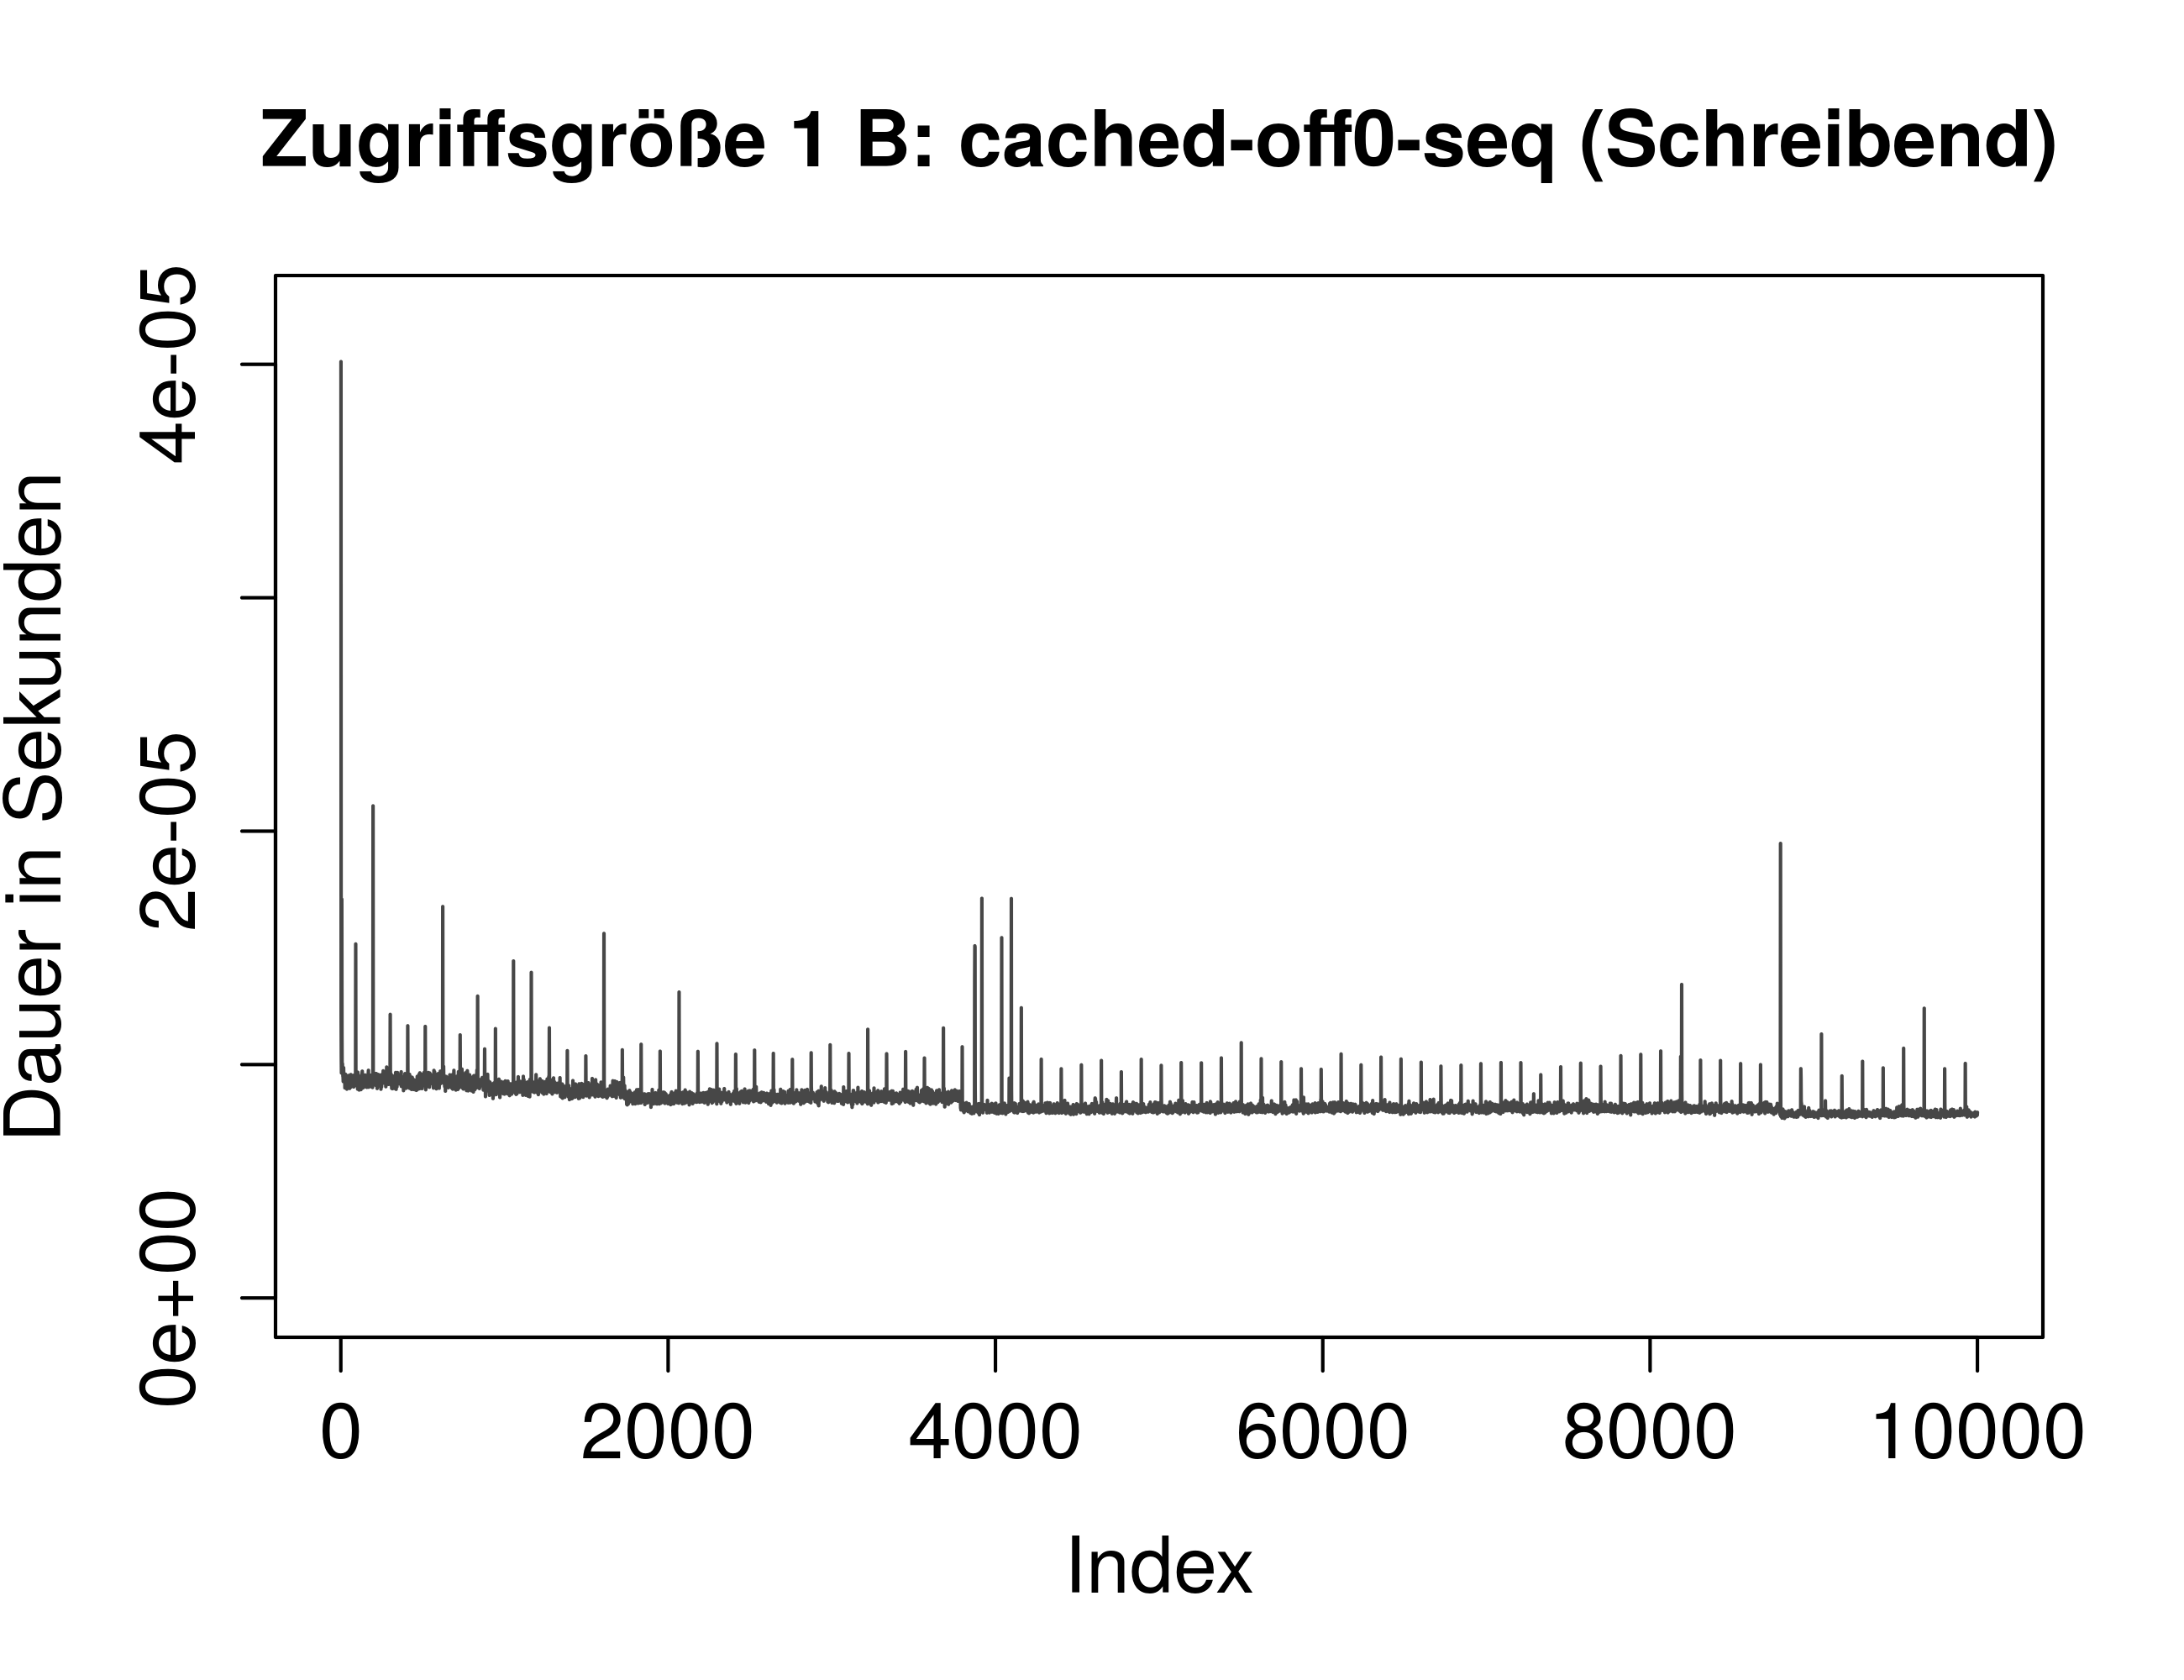
\includegraphics[width=.43\textwidth]{Bilder/Plots/exploration/plot_Size1_write_seq.png}
	}\\
	\subfloat{
		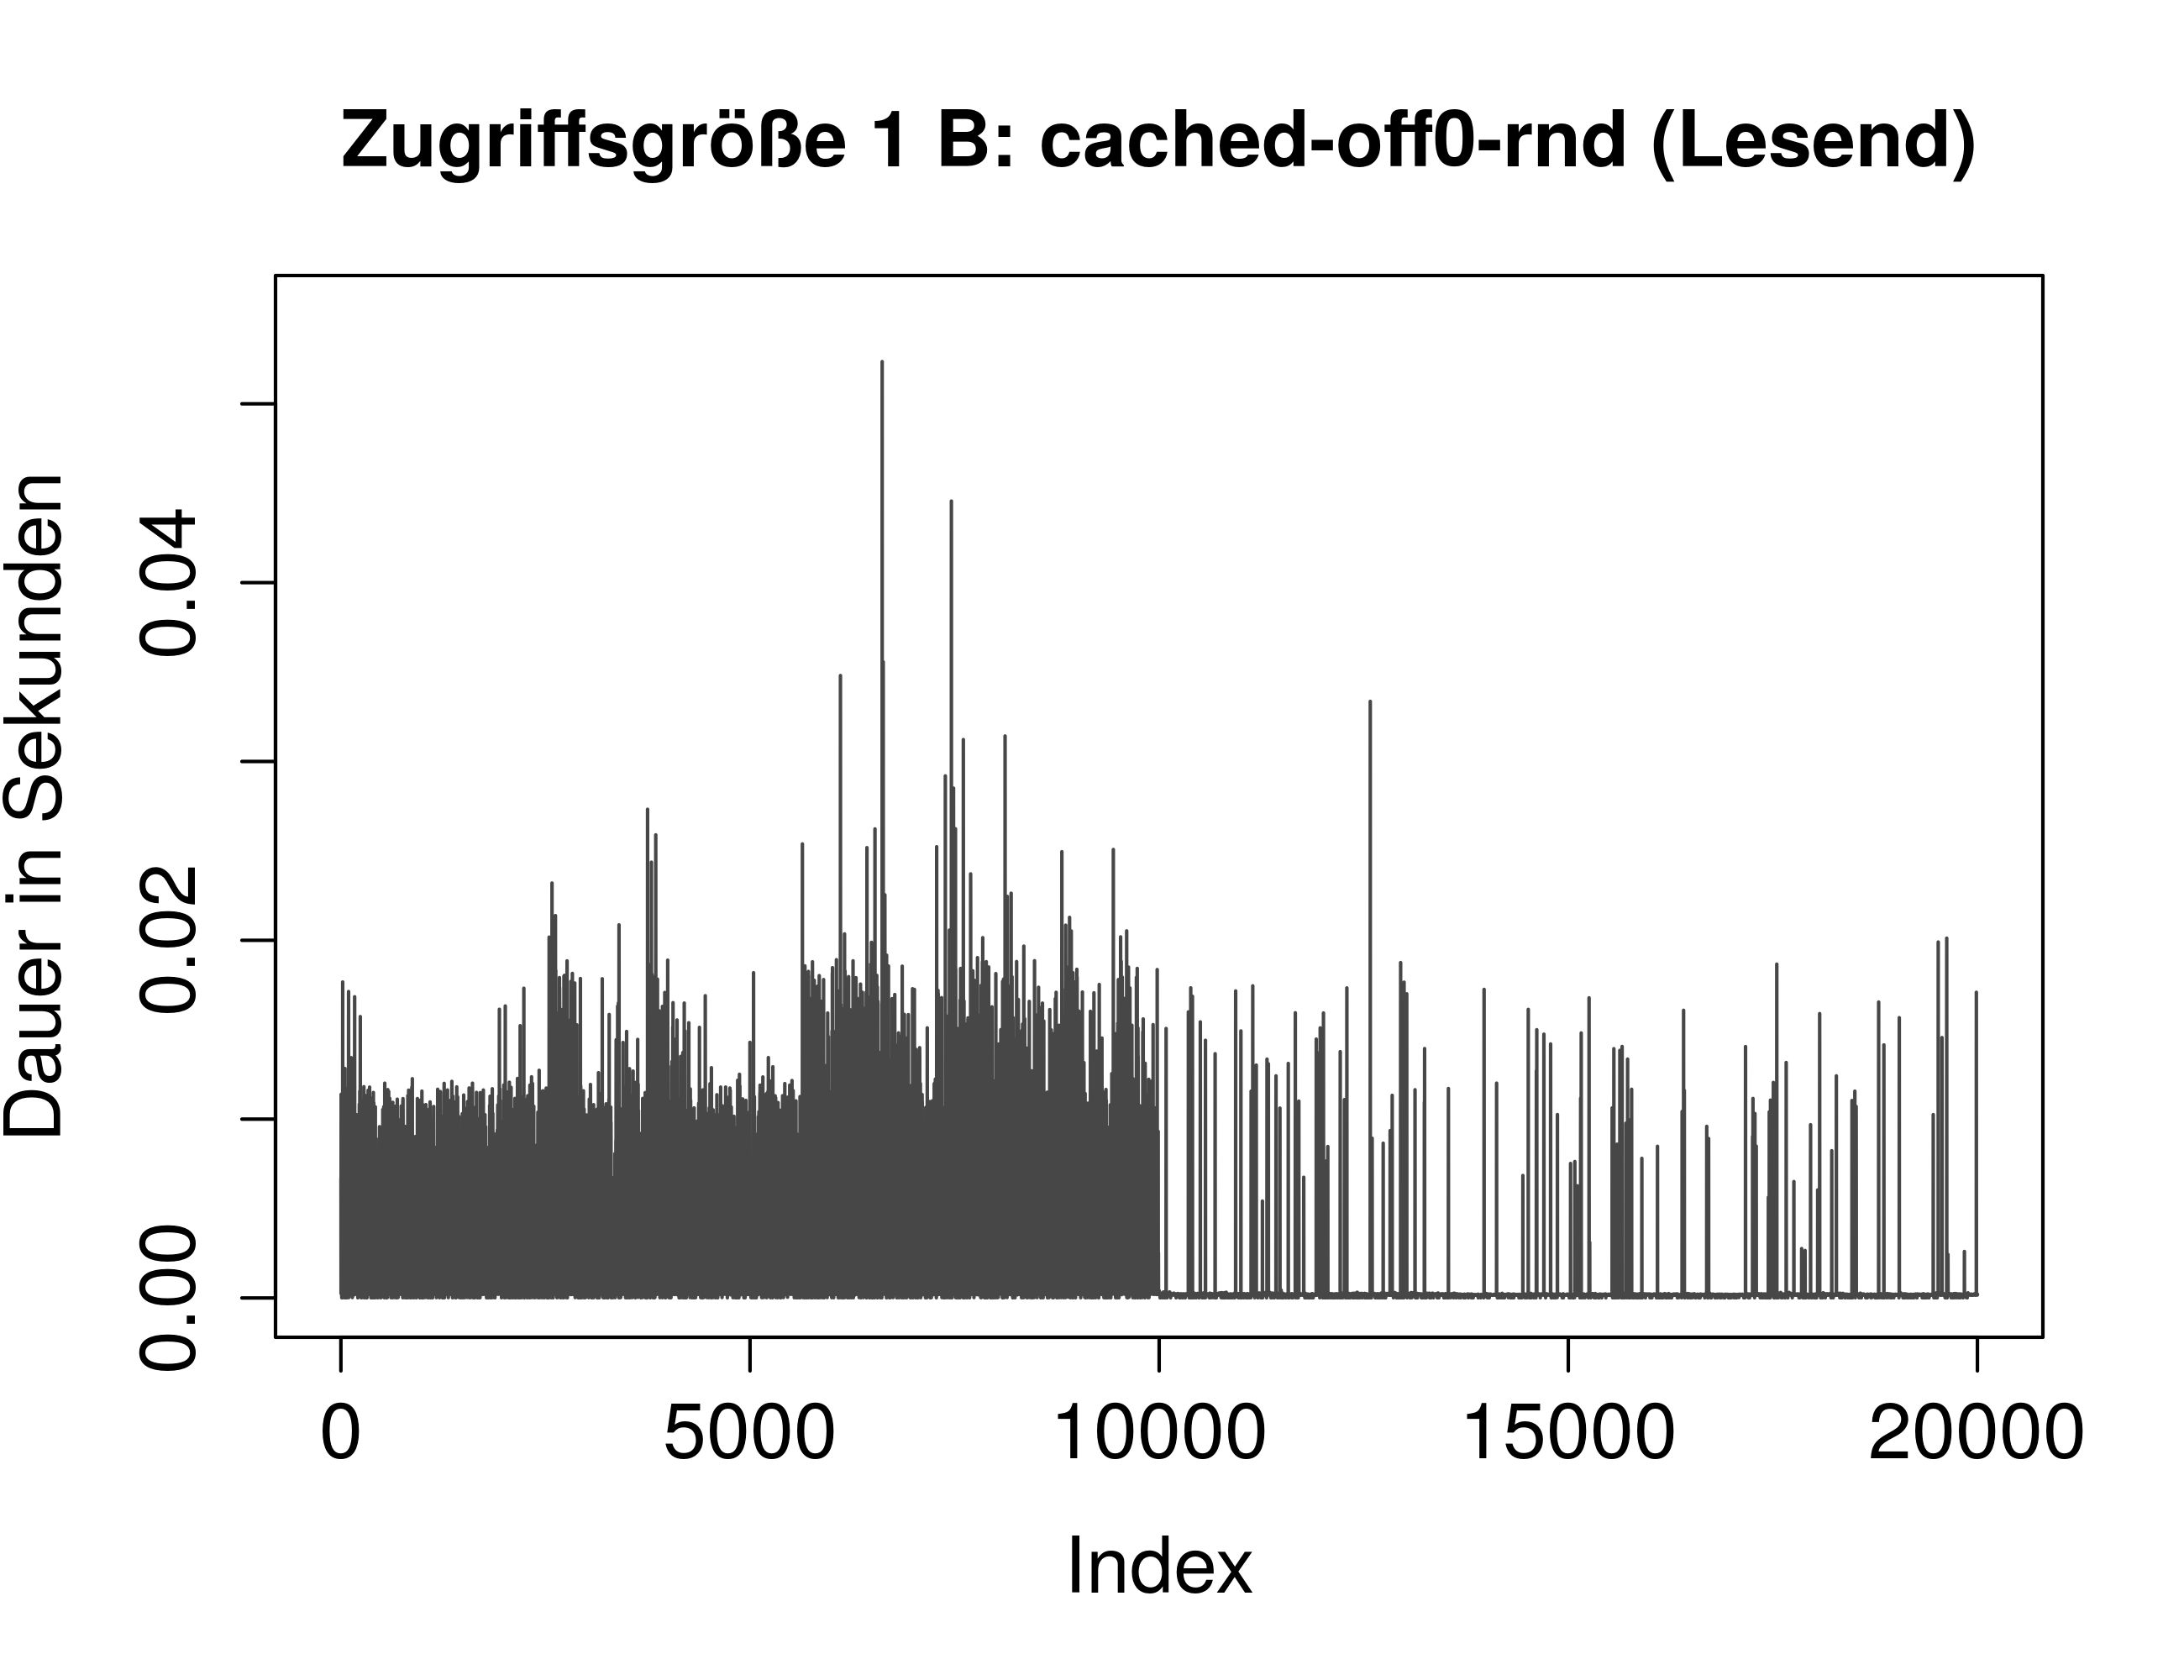
\includegraphics[width=.43\textwidth]{Bilder/Plots/exploration/plot_Size1_read_rnd.png}
	}
	\hfill
	\subfloat{
		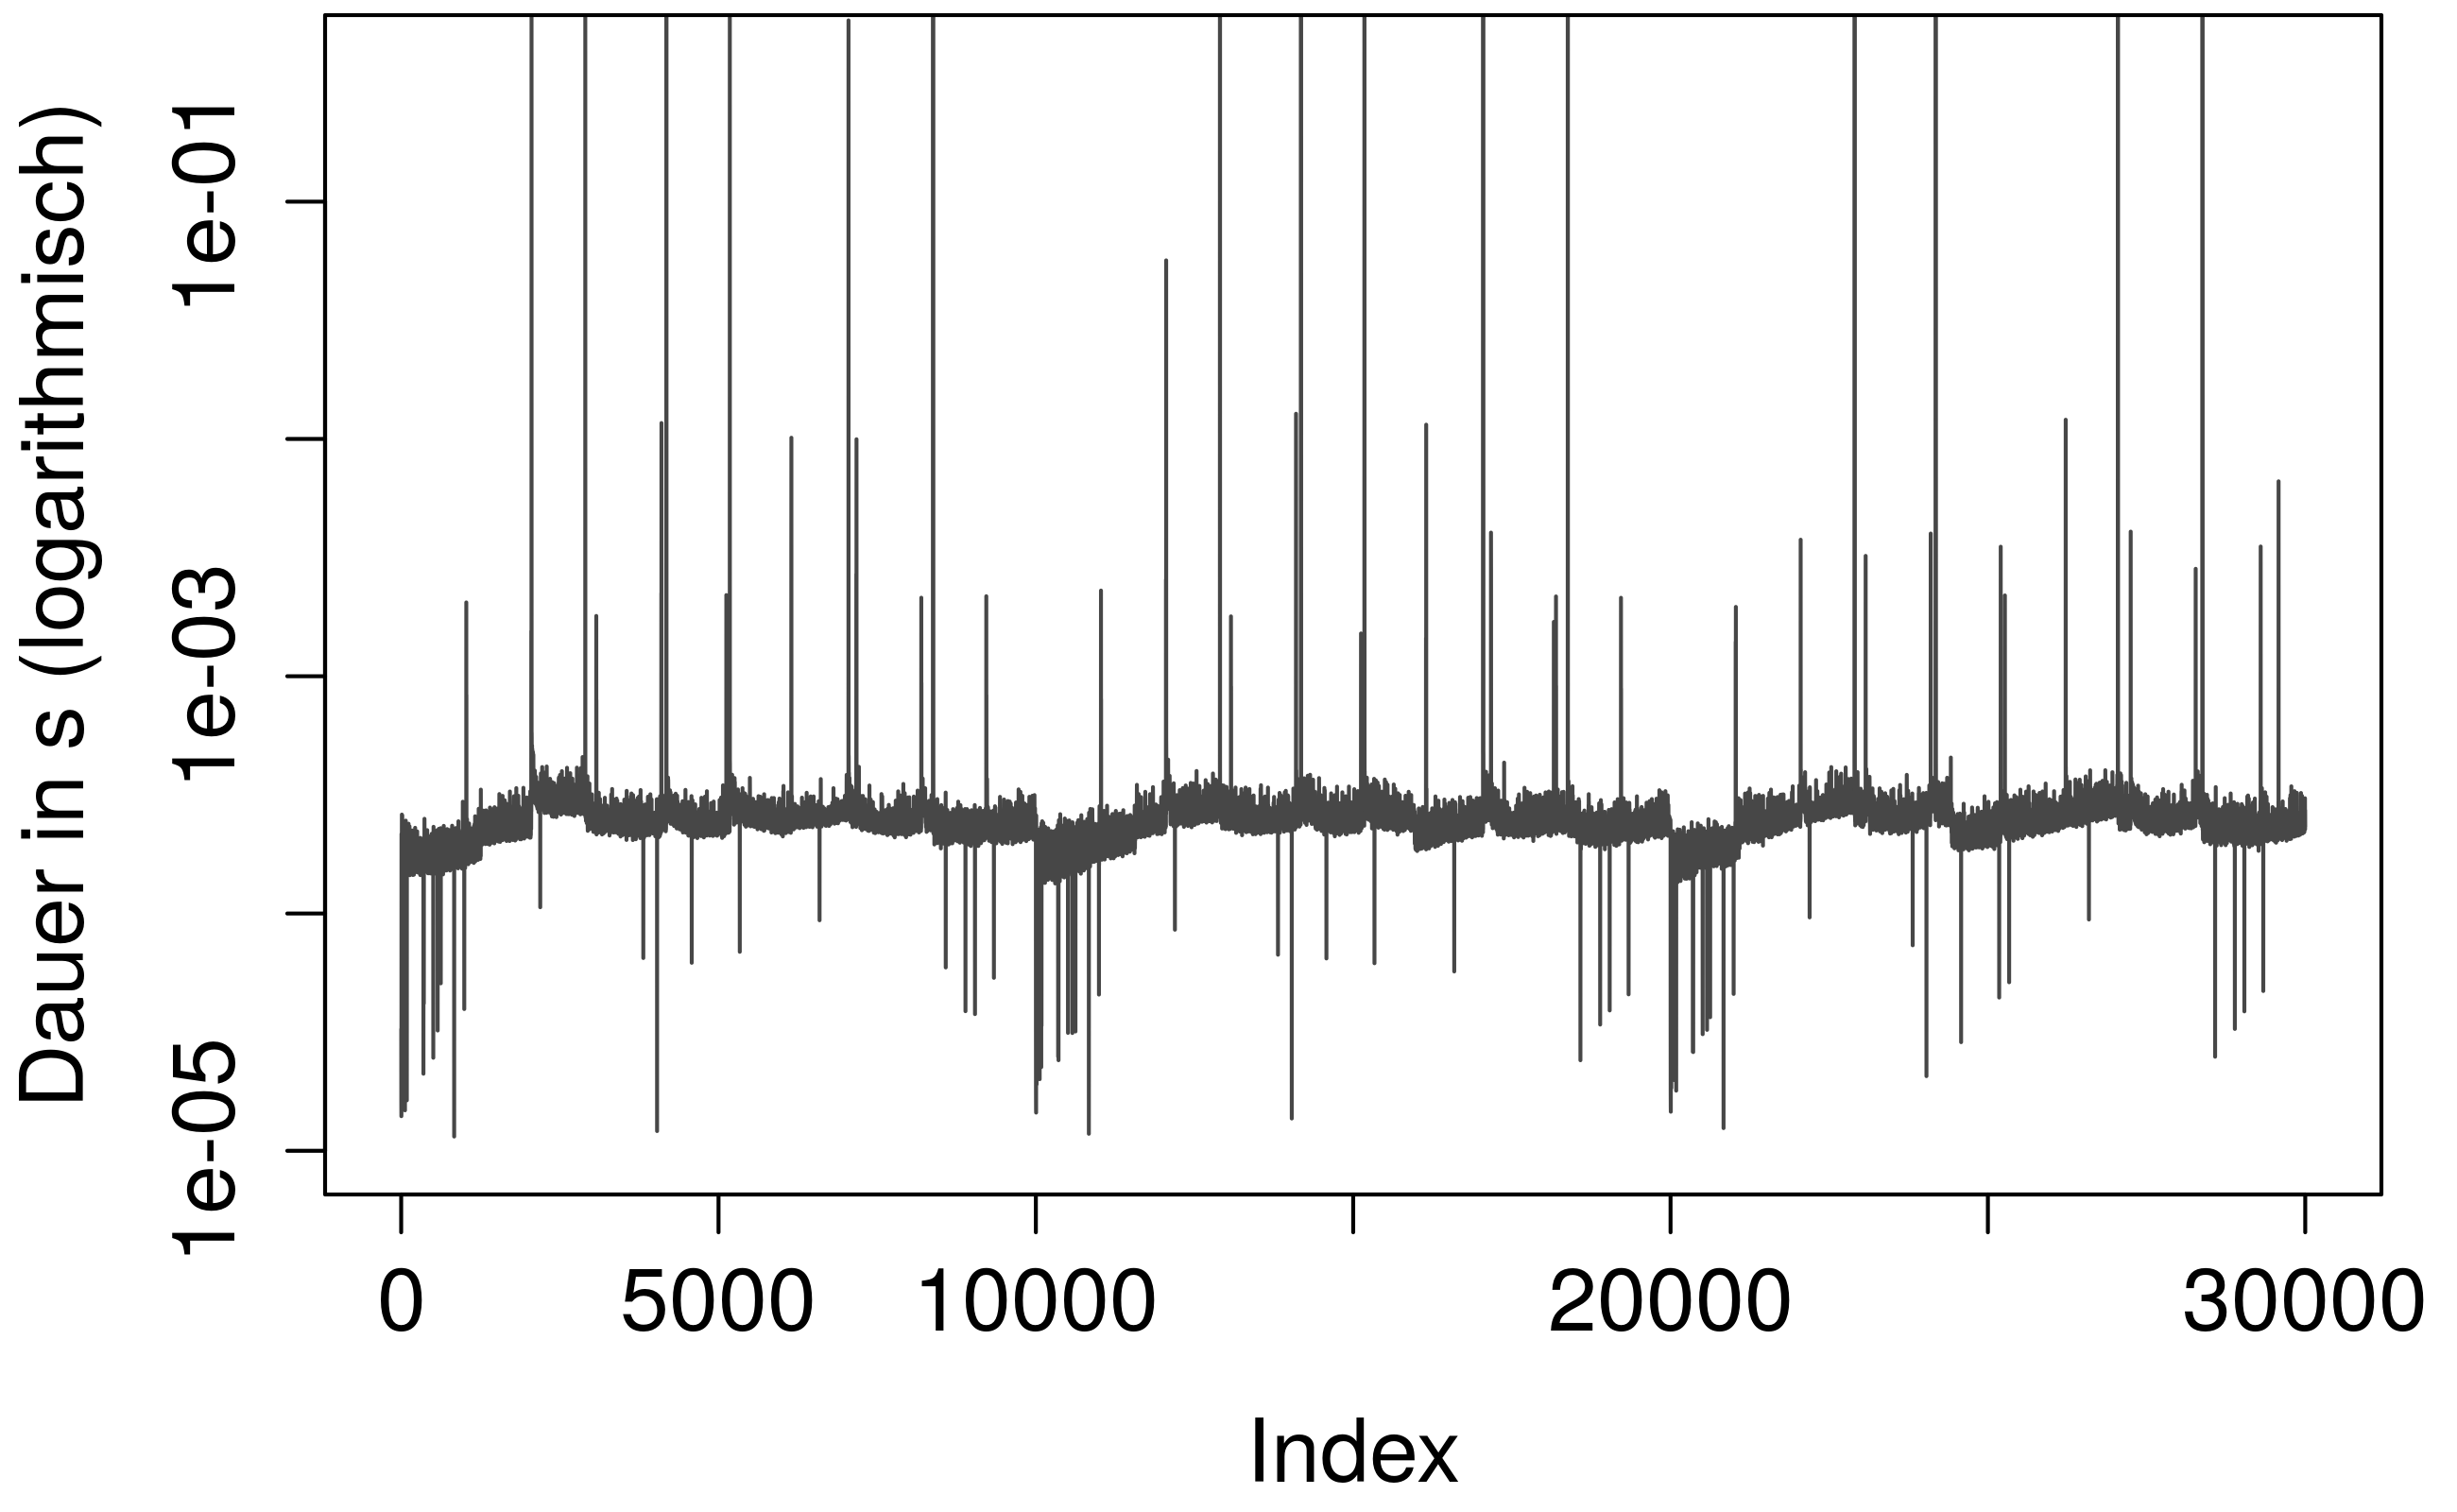
\includegraphics[width=.43\textwidth]{Bilder/Plots/exploration/plot_Size1_write_rnd.png}
	}		
	\caption{Detailbetrachtung aller Messungen mit Zugriffsgröße 1KB}
	\label{fig:groesse1}
\end{figure} 

\begin{figure}
	\subfloat{
		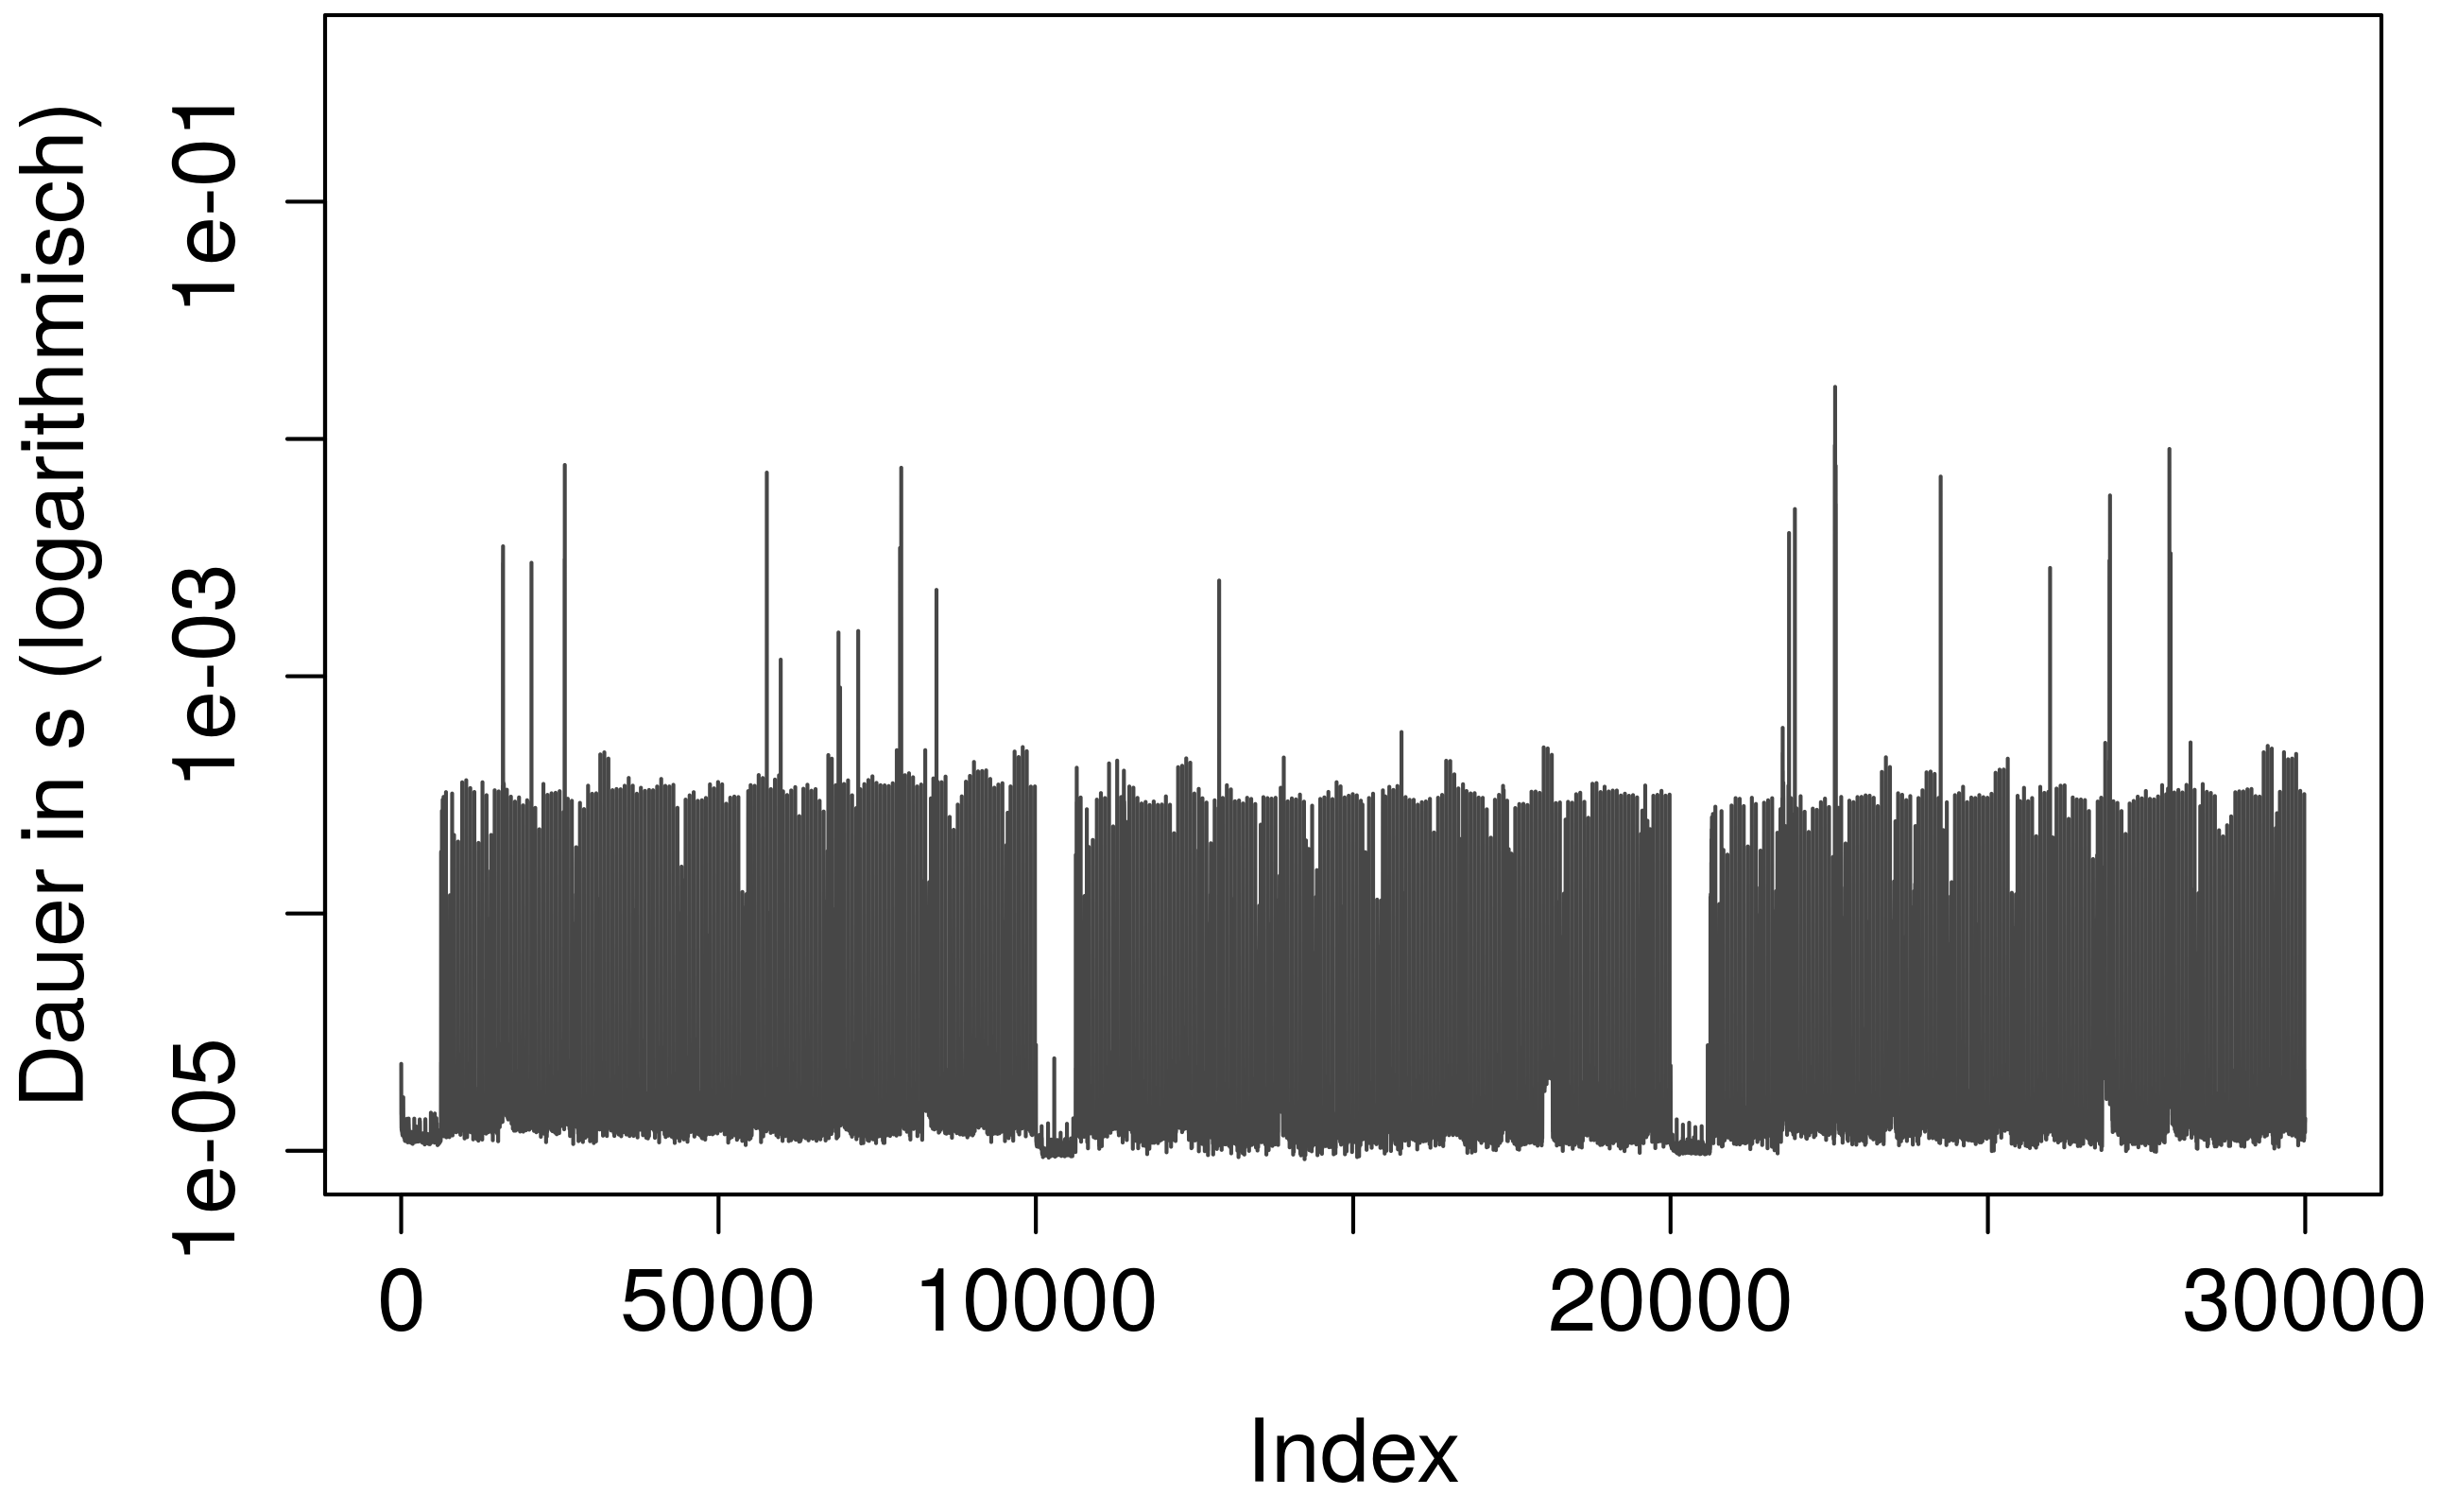
\includegraphics[width=.43\textwidth]{Bilder/Plots/exploration/plot_Size16384_read_seq.png}
	}
	\hfill
	\subfloat{
		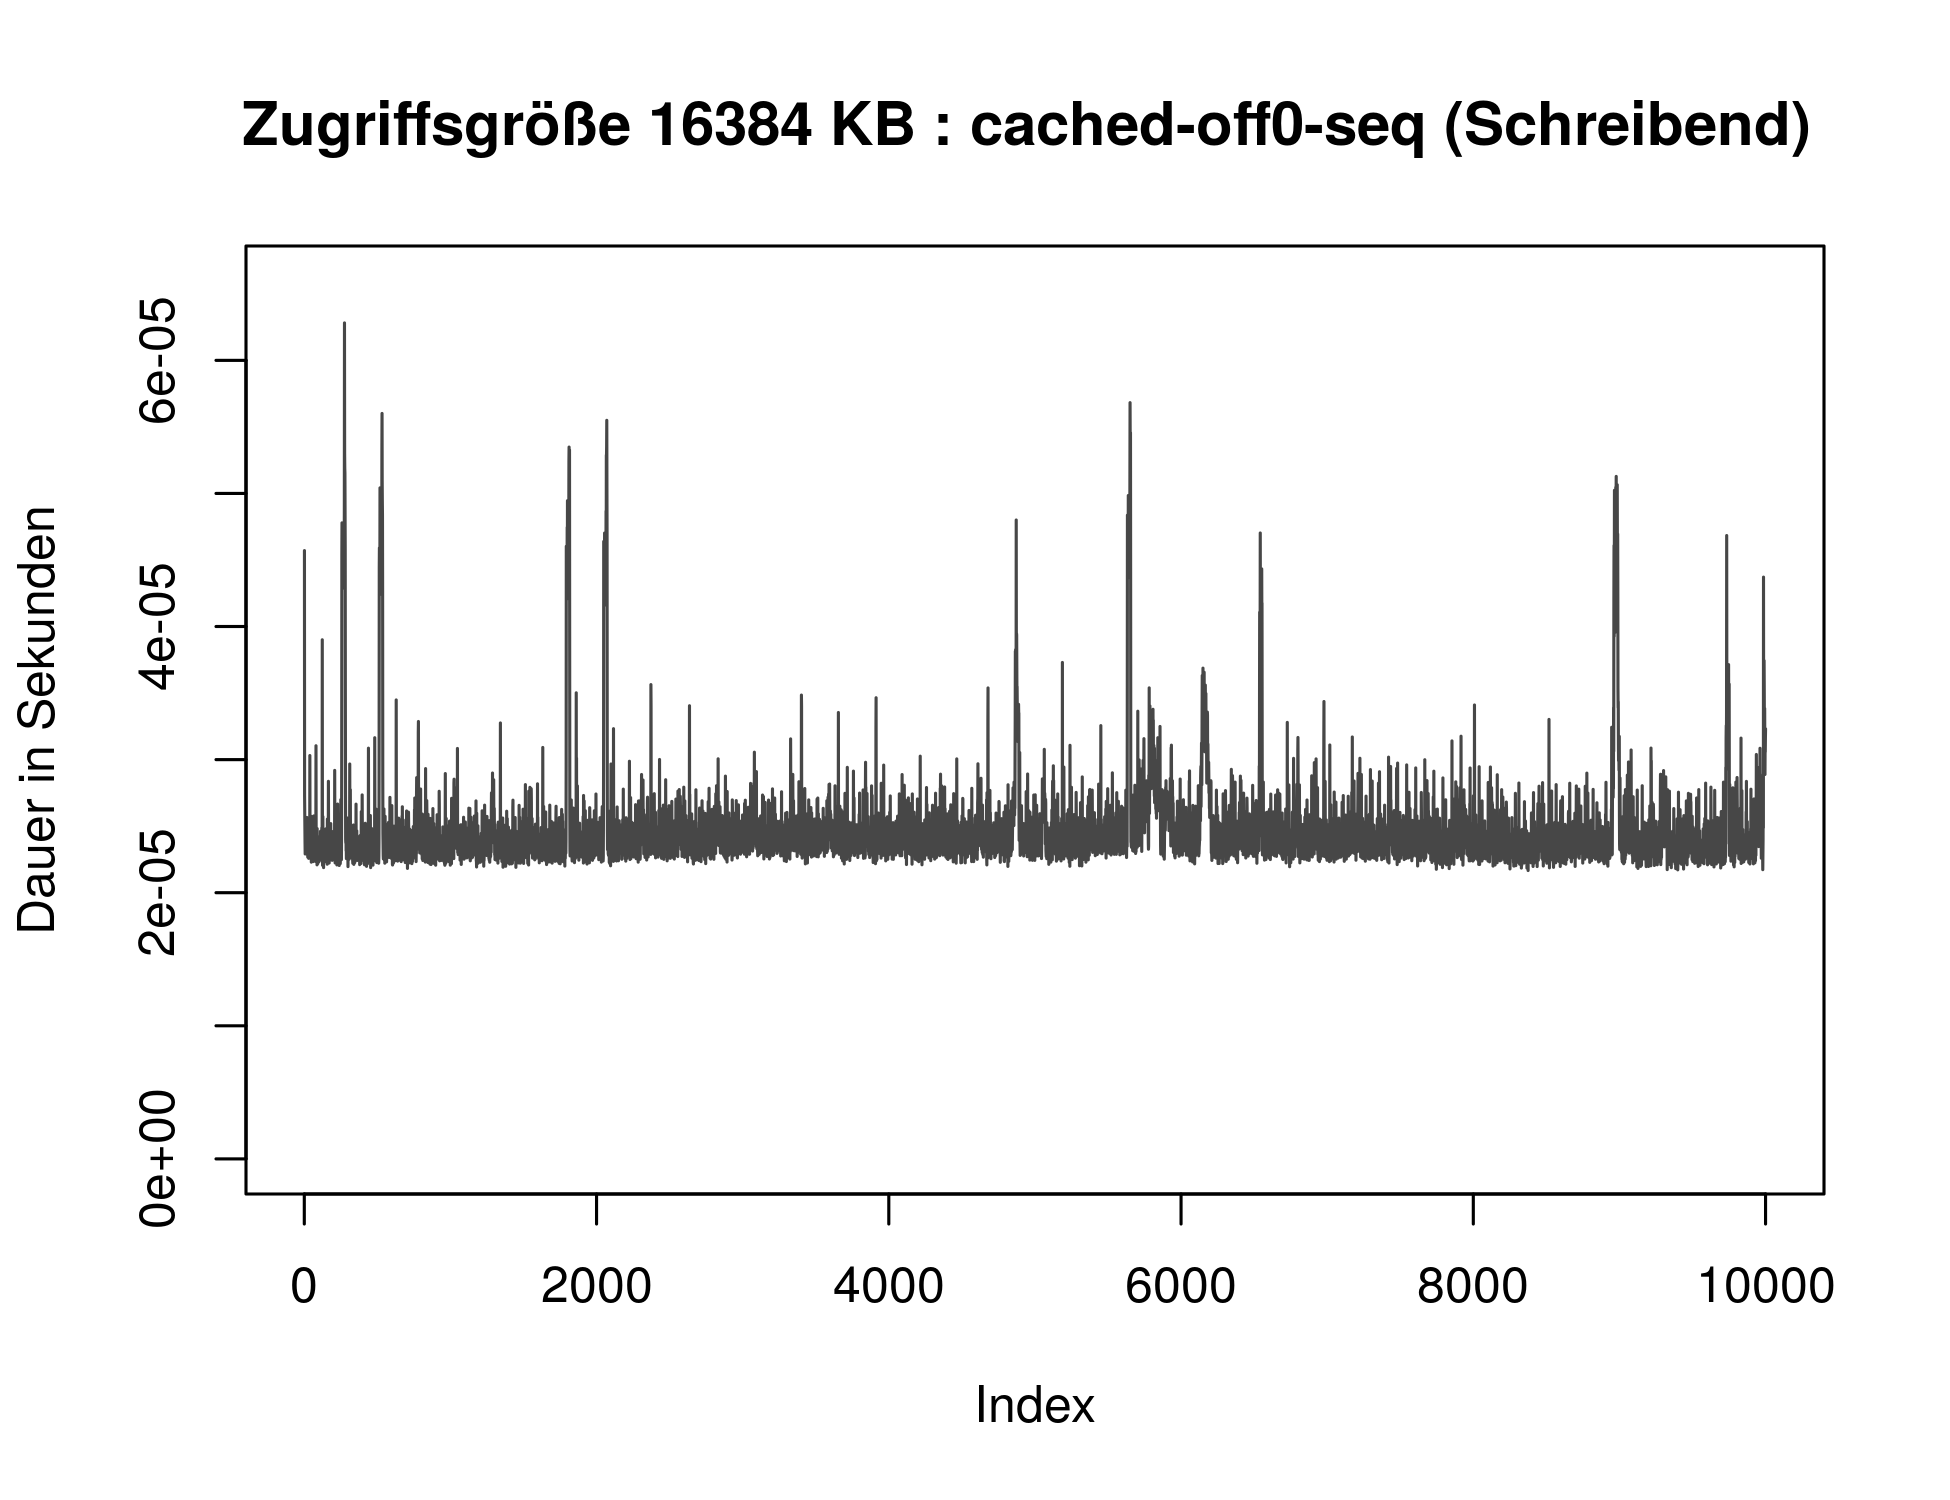
\includegraphics[width=.43\textwidth]{Bilder/Plots/exploration/plot_Size16384_write_seq.png}
	}\\
	\subfloat{
		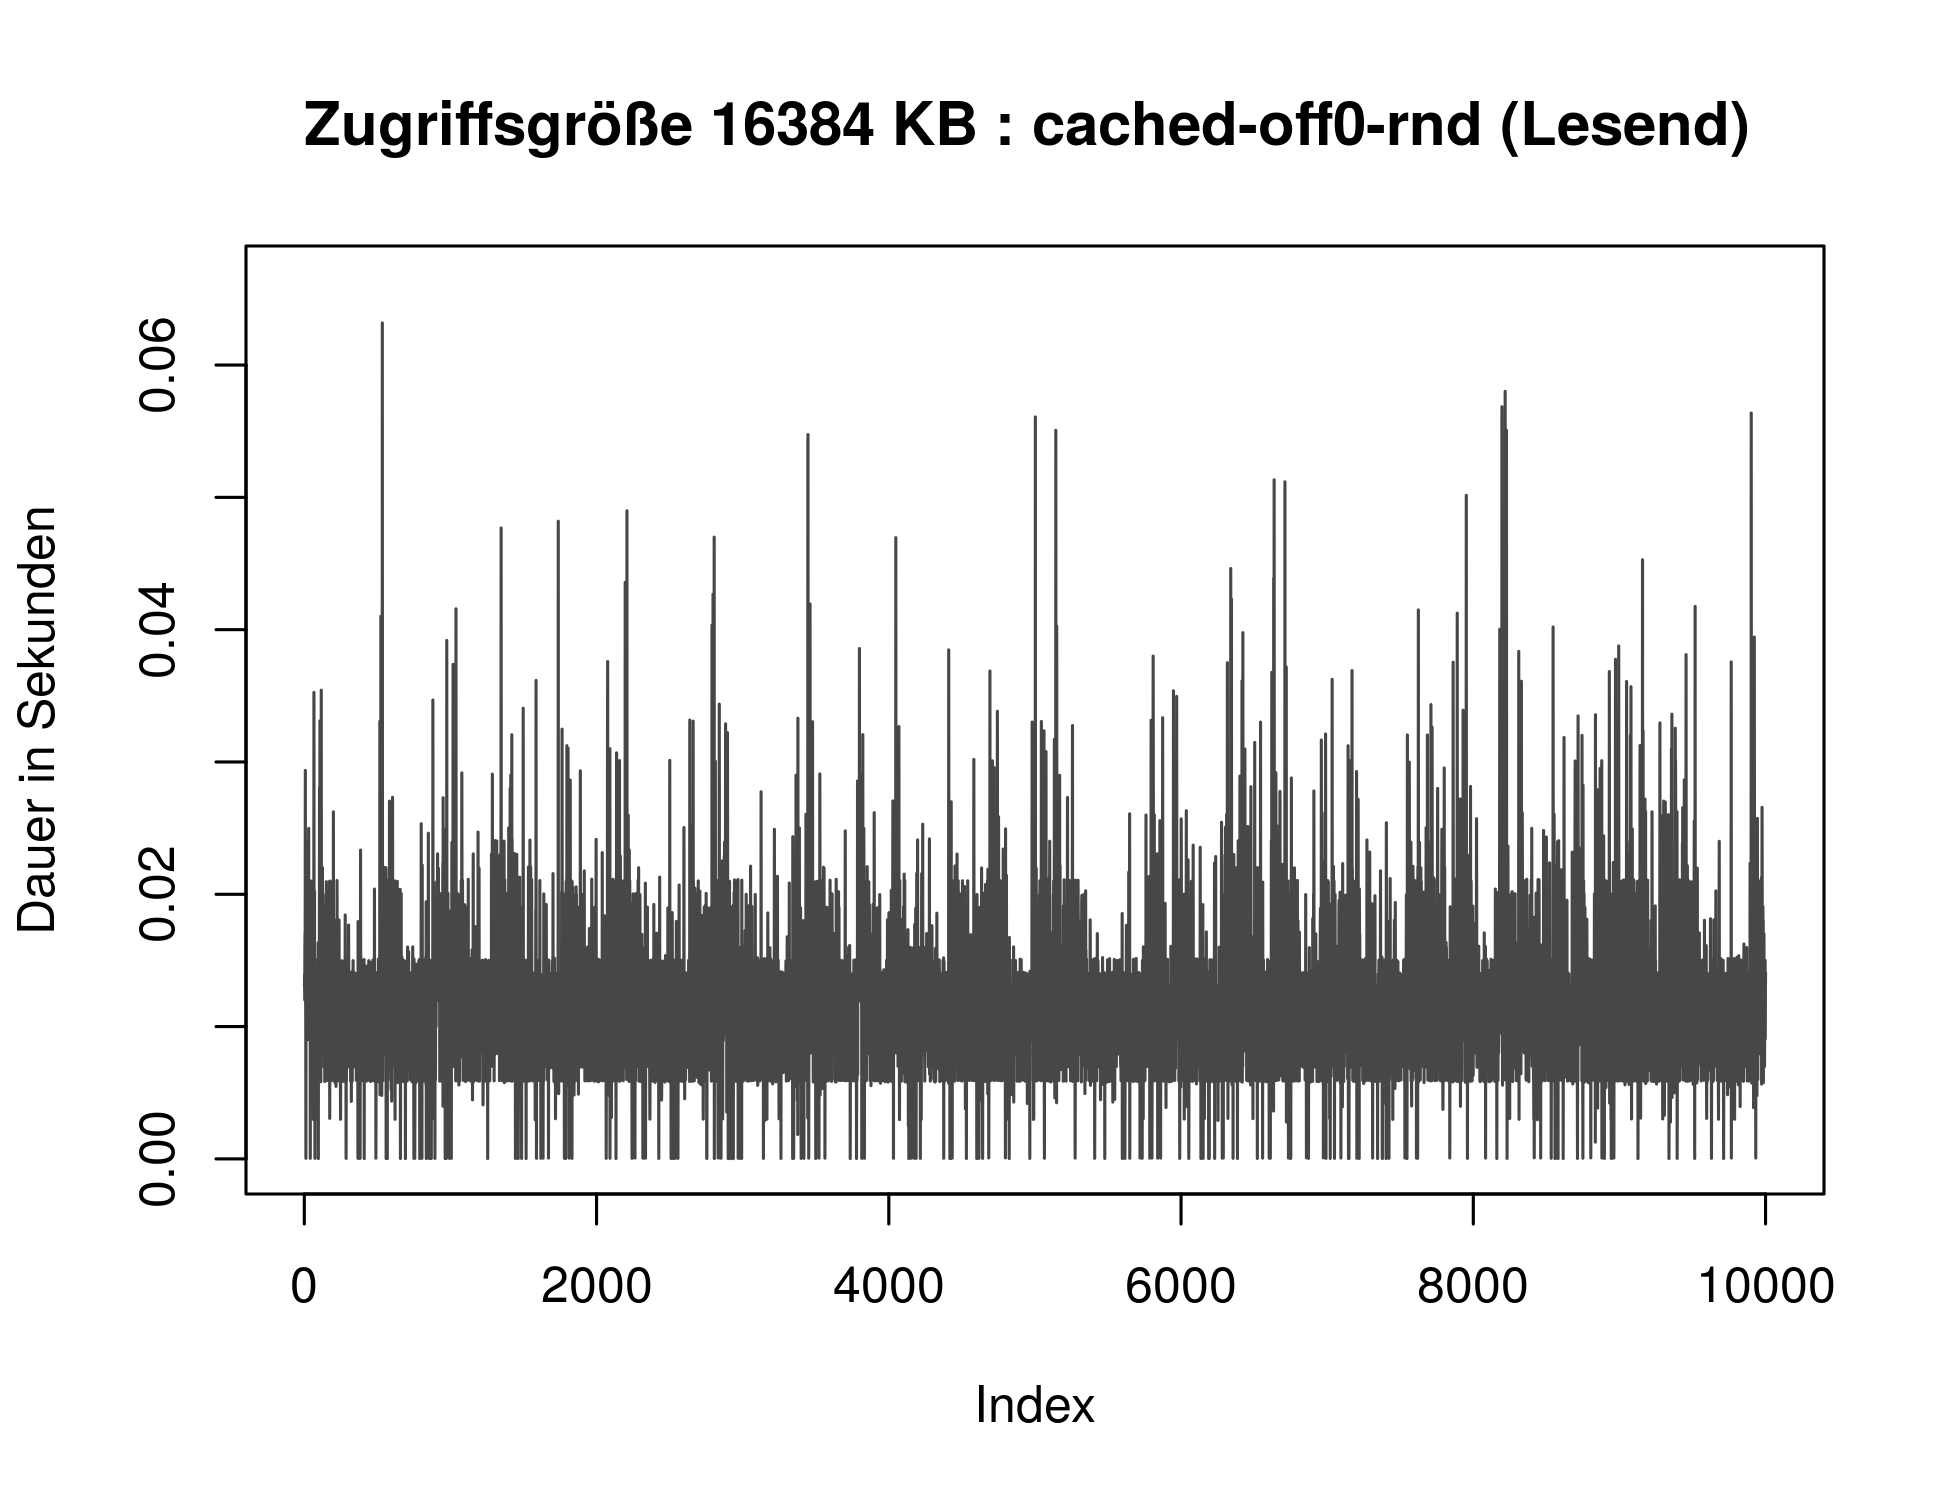
\includegraphics[width=.43\textwidth]{Bilder/Plots/exploration/plot_Size16384_read_rnd.png}
	}
	\hfill
	\subfloat{
		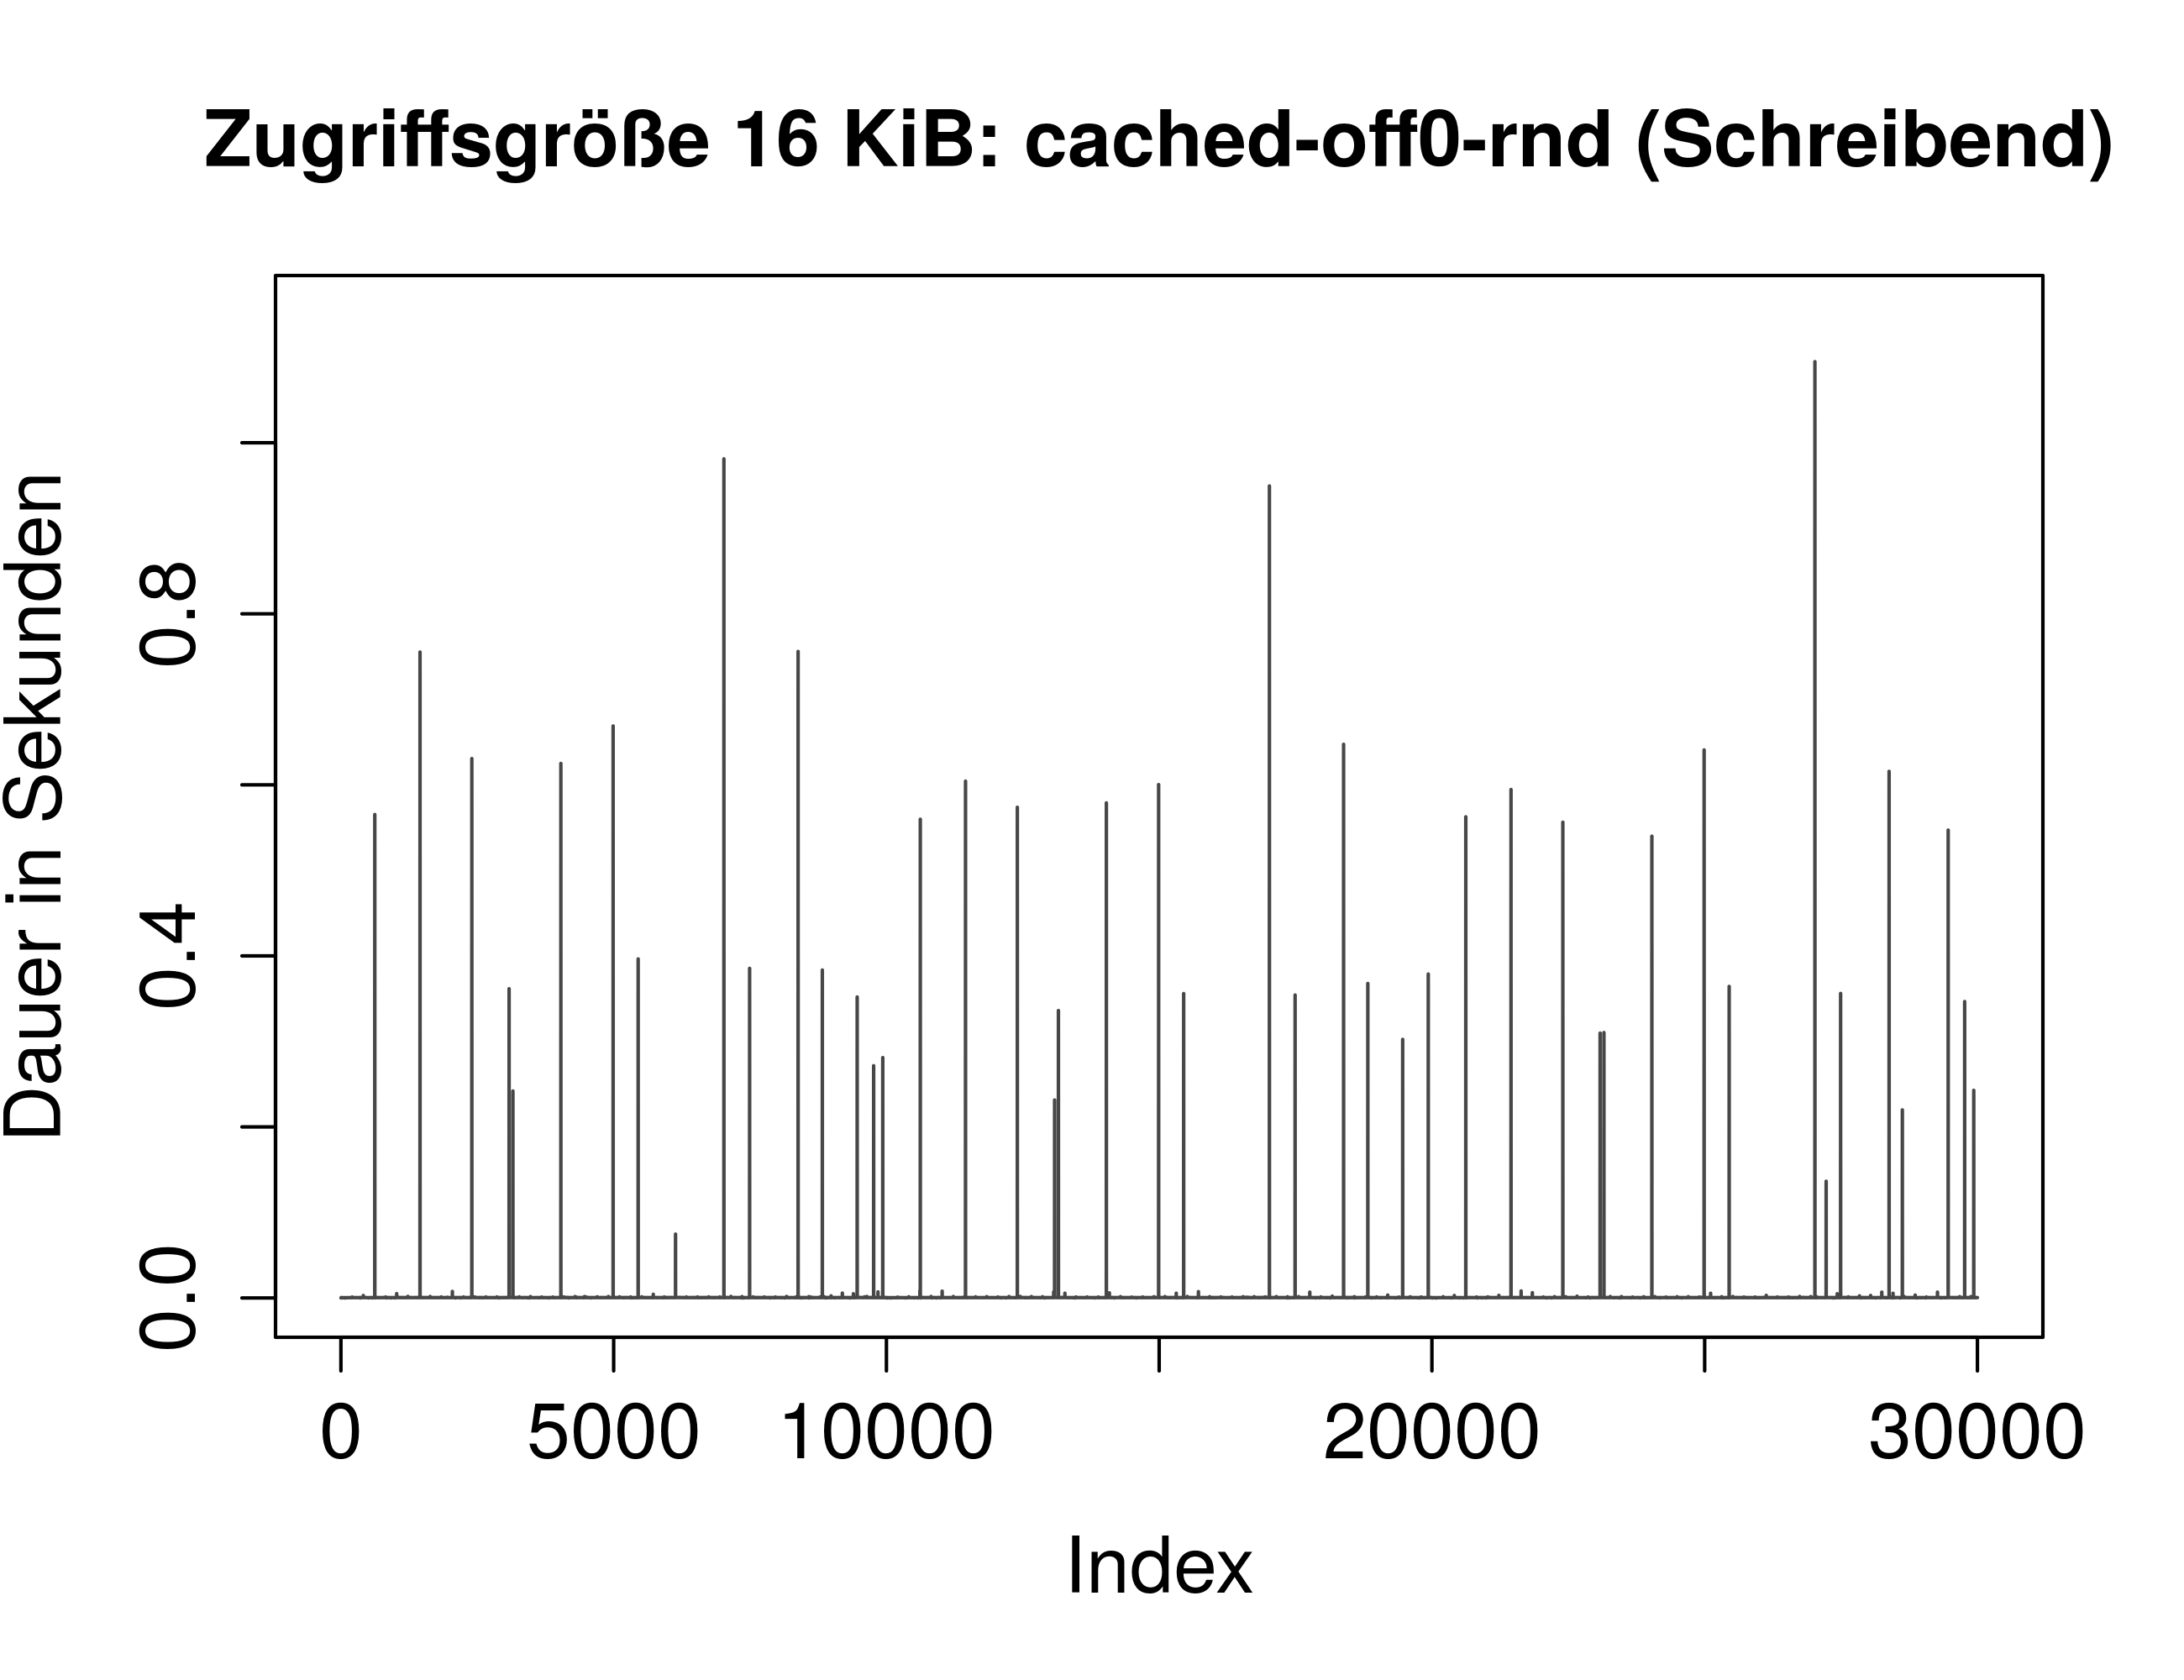
\includegraphics[width=.43\textwidth]{Bilder/Plots/exploration/plot_Size16384_write_rnd.png}
	}		
	\caption{Detailbetrachtung aller Messungen mit Zugriffsgröße 16384KB}
	\label{fig:groesse16384}
\end{figure} 

\begin{figure}
	\subfloat{
		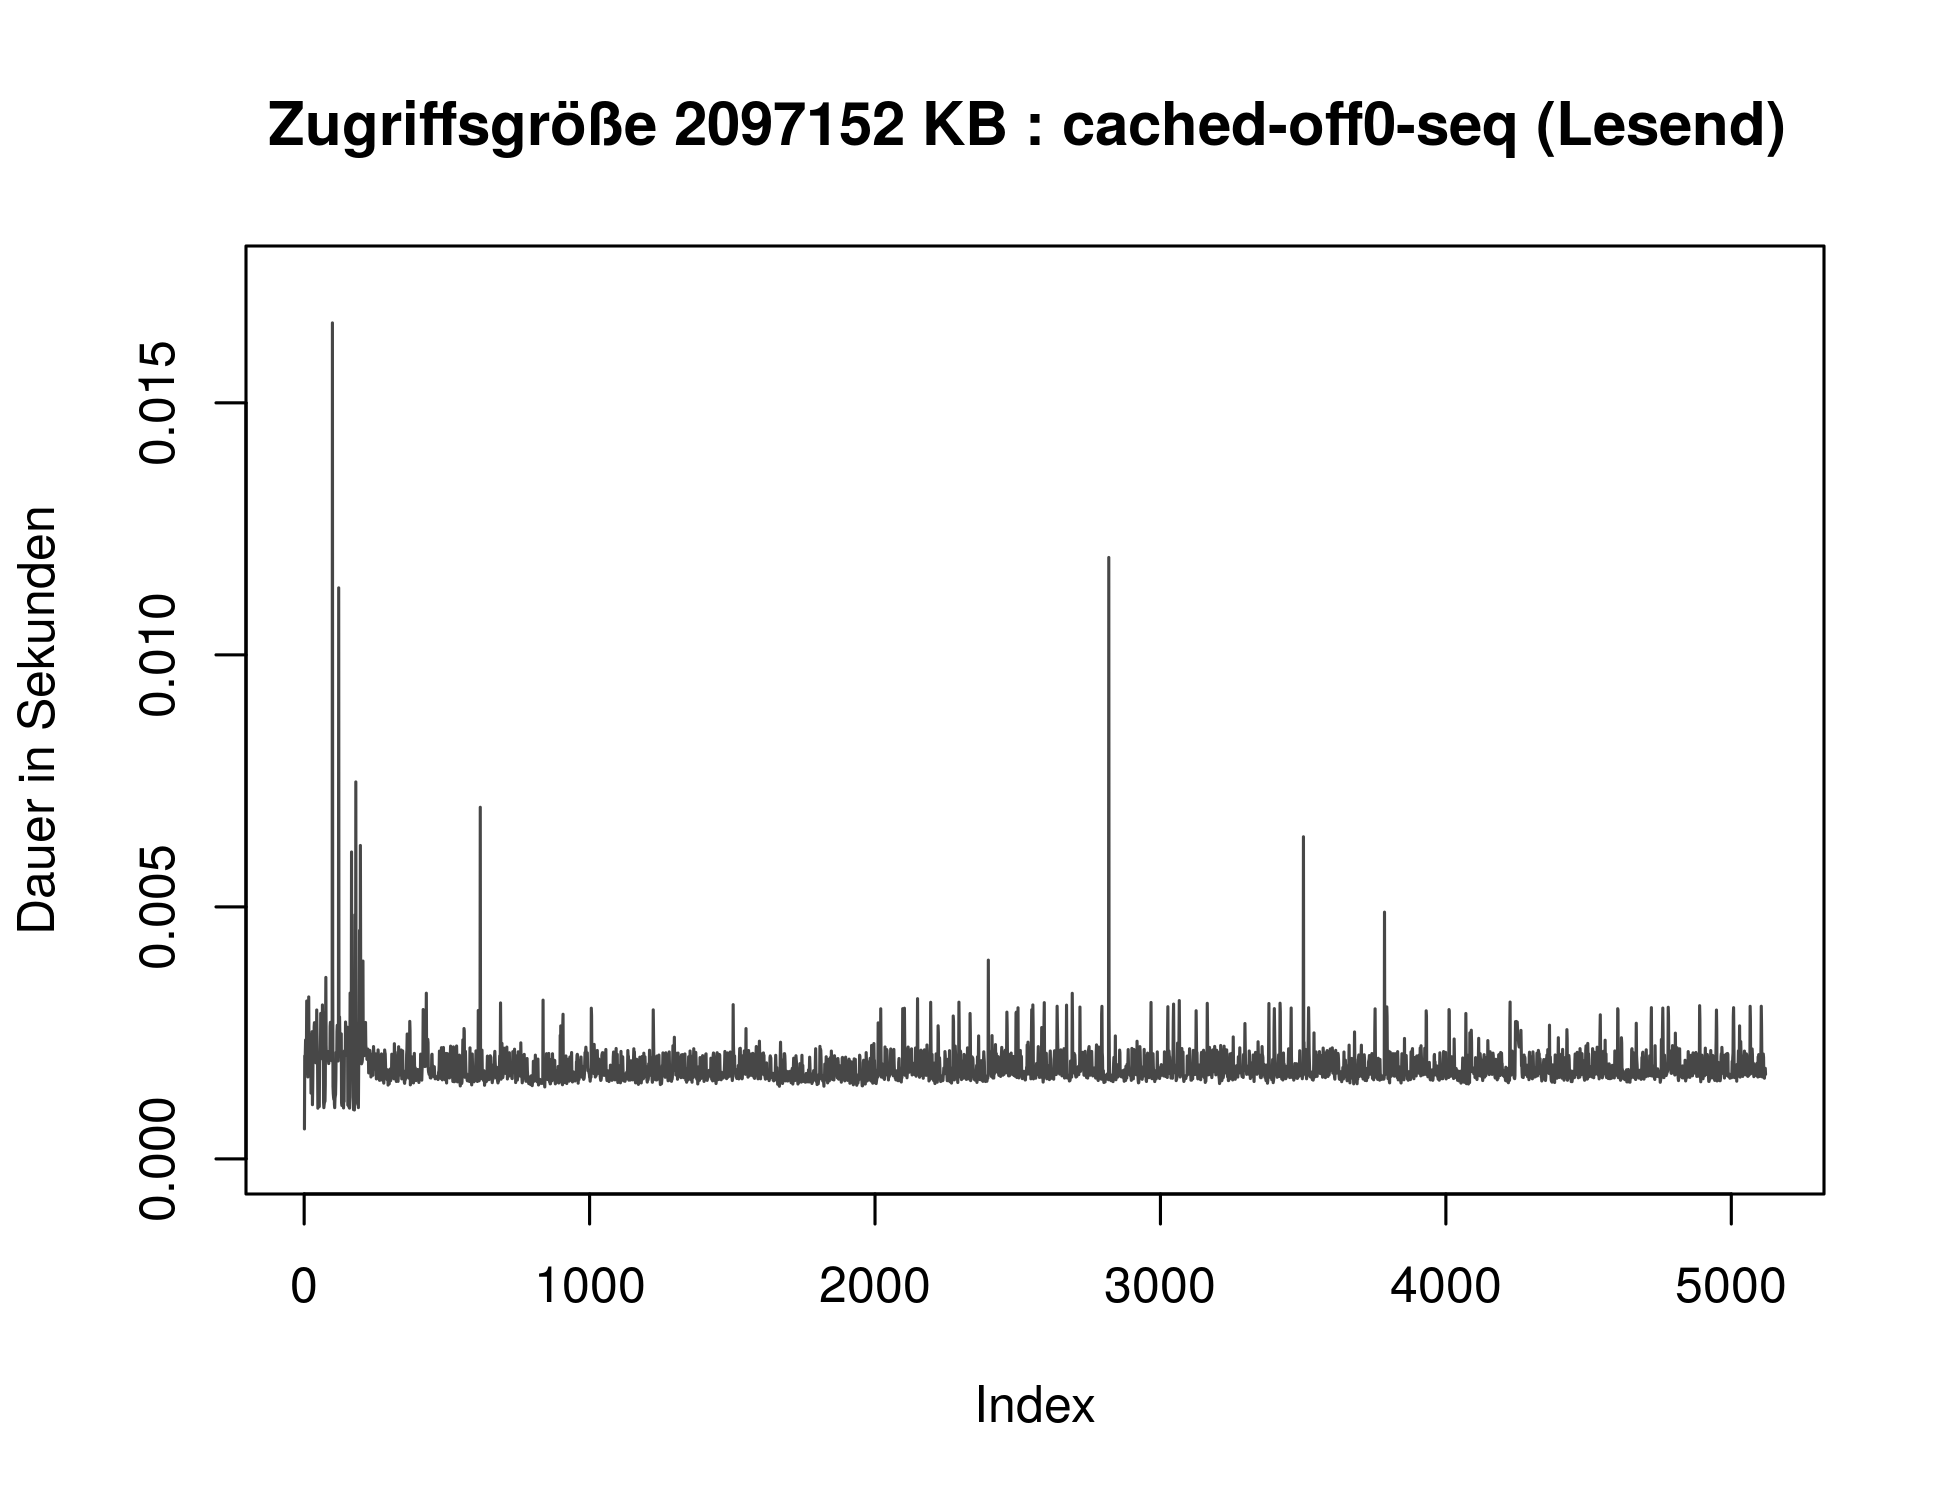
\includegraphics[width=.43\textwidth]{Bilder/Plots/exploration/plot_Size2097152_read_seq.png}
	}
	\hfill
	\subfloat{
		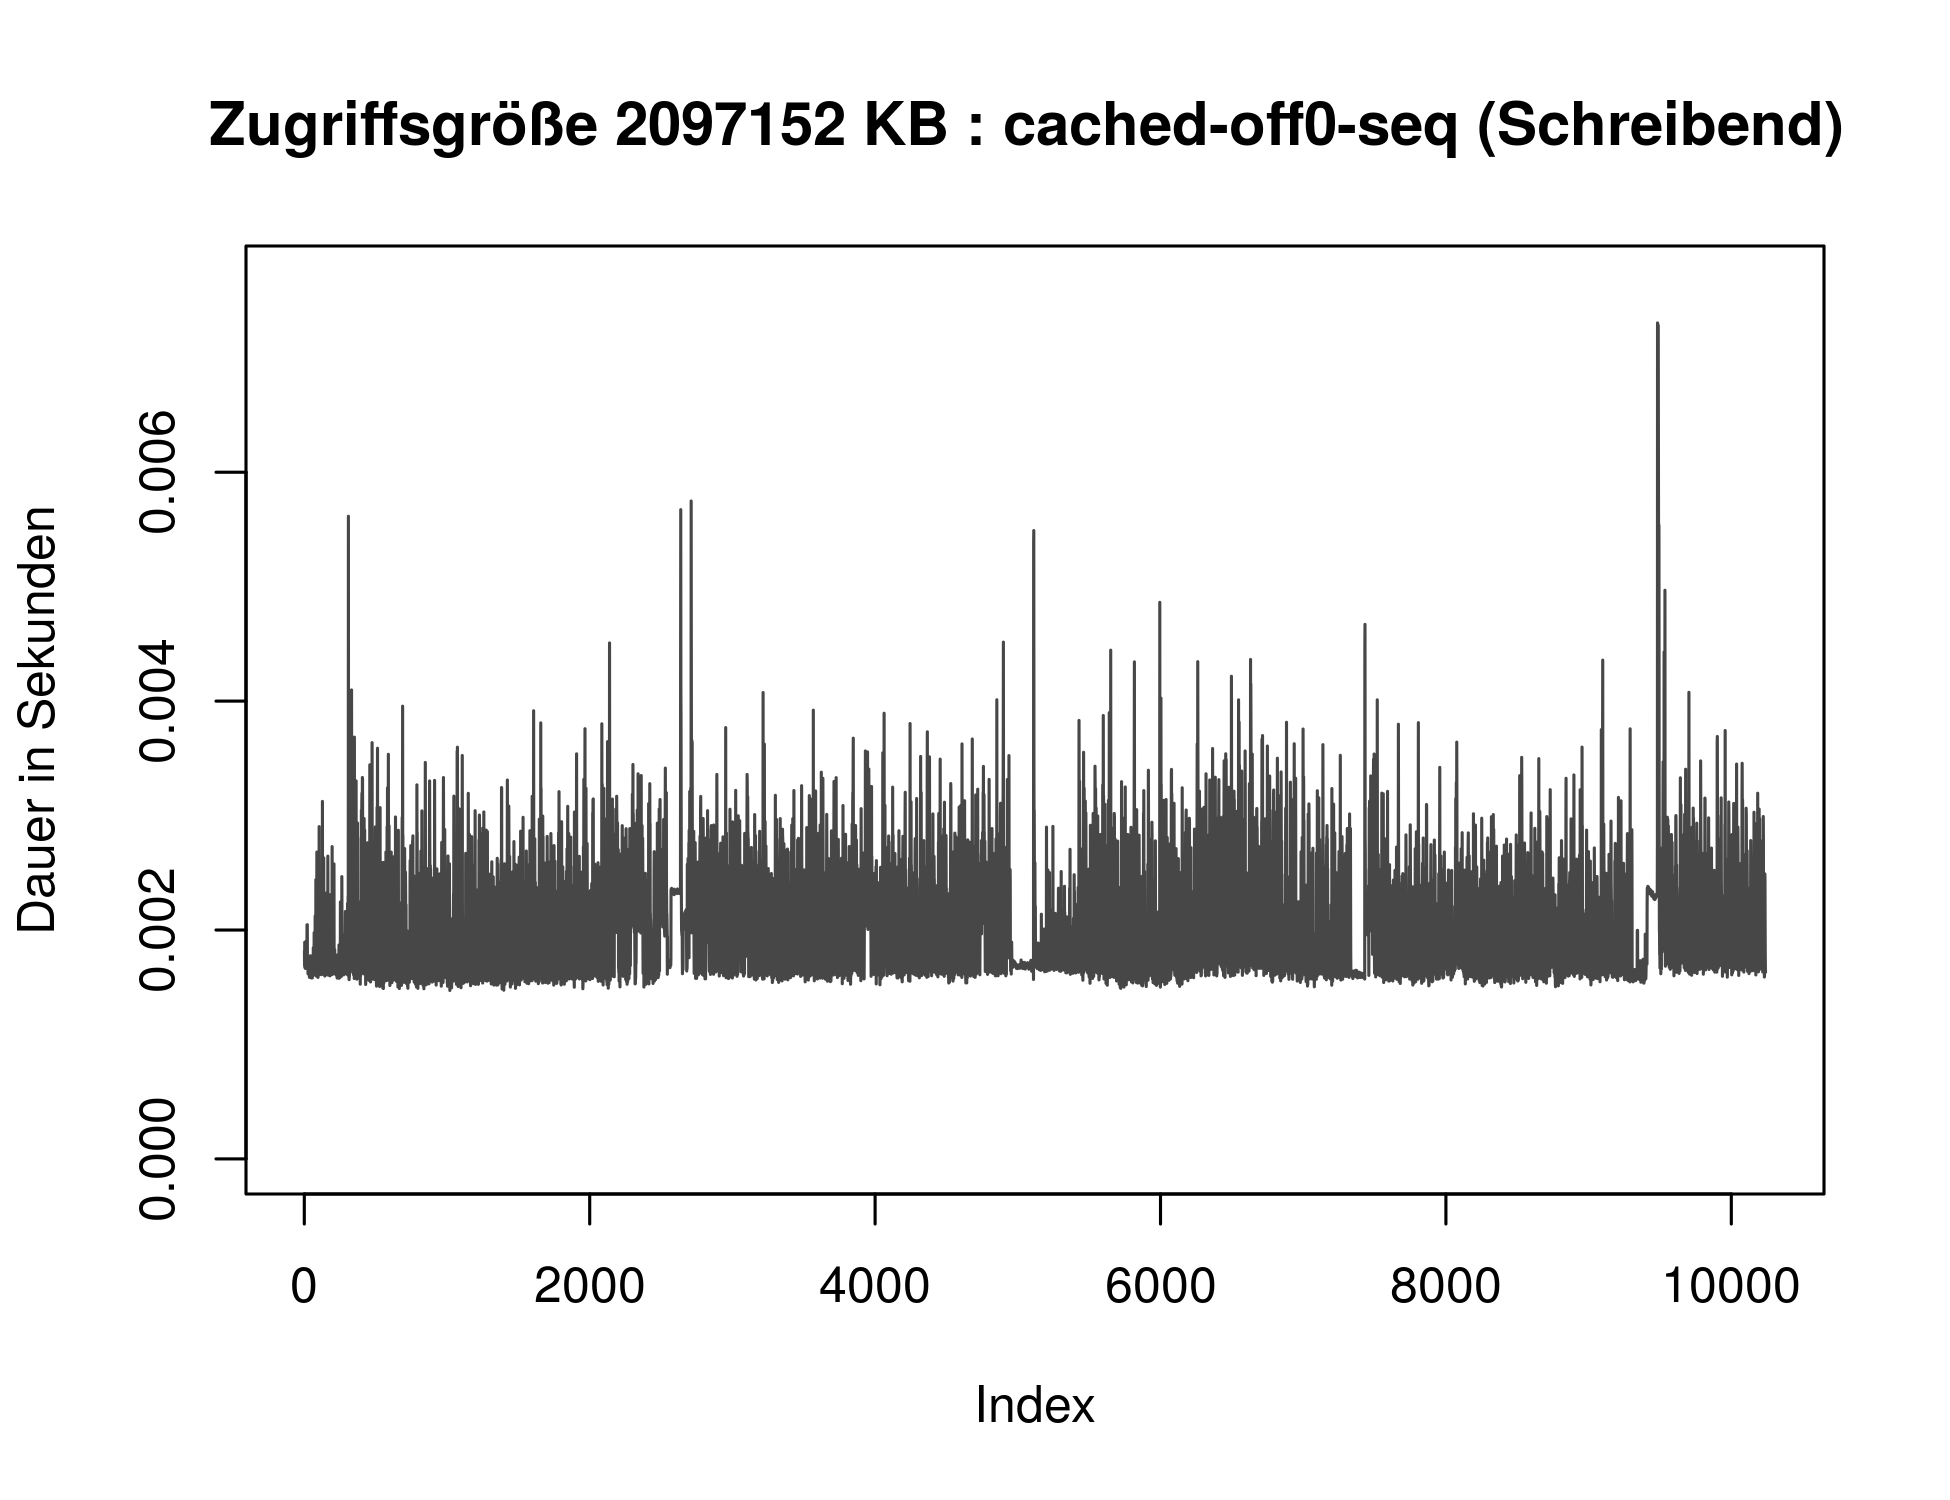
\includegraphics[width=.43\textwidth]{Bilder/Plots/exploration/plot_Size2097152_write_seq.png}
	}\\
	\subfloat{
		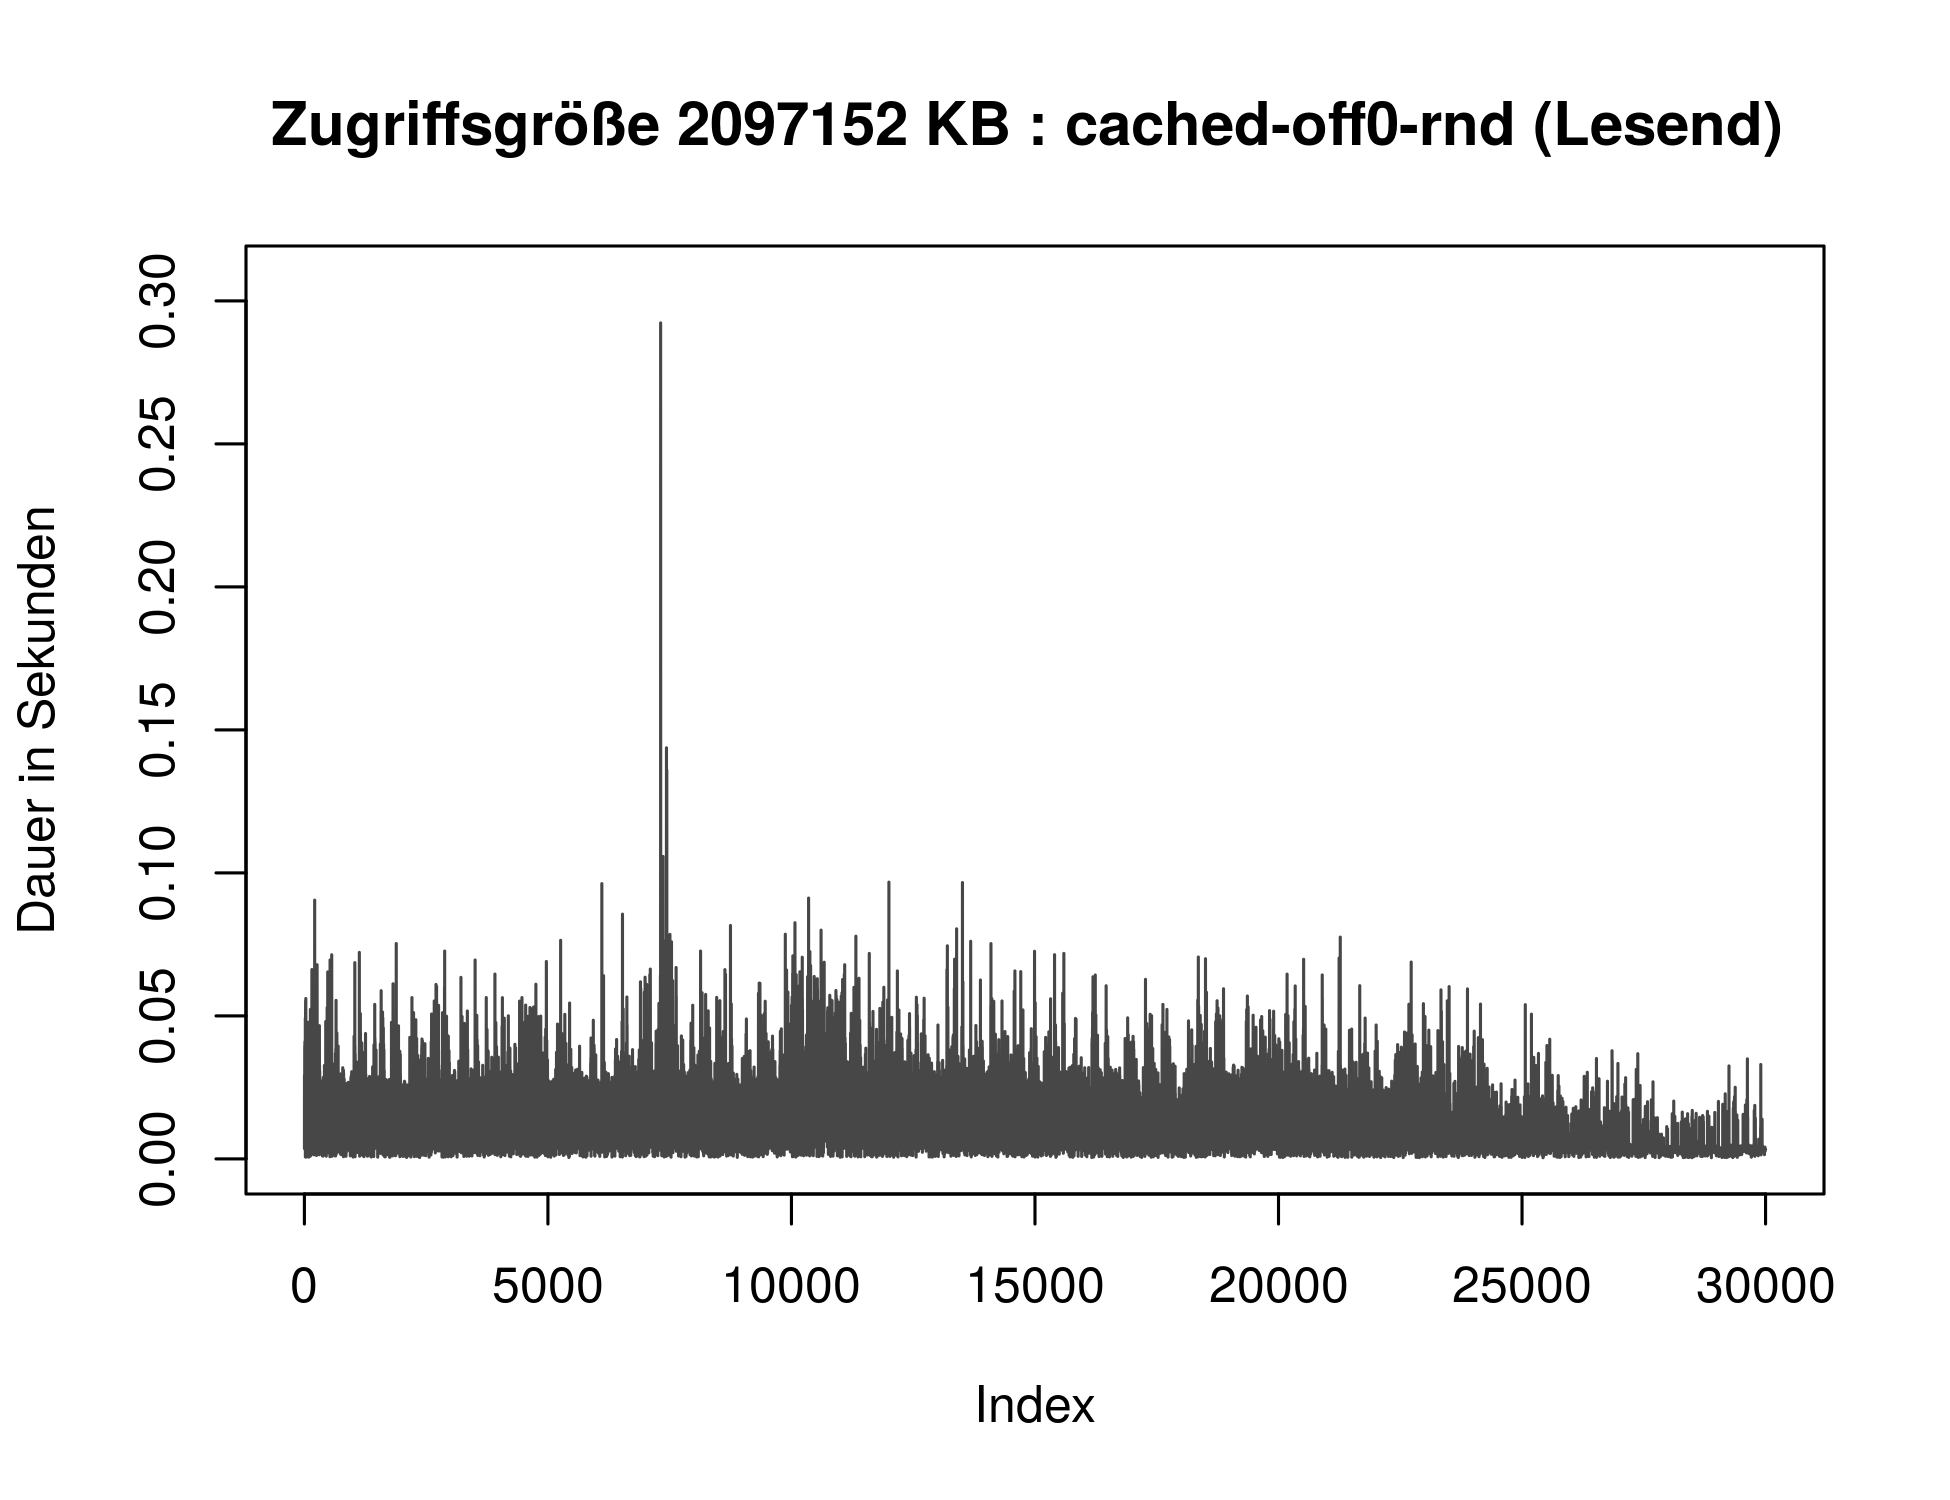
\includegraphics[width=.43\textwidth]{Bilder/Plots/exploration/plot_Size2097152_read_rnd.png}
	}
	\hfill
	\subfloat{
		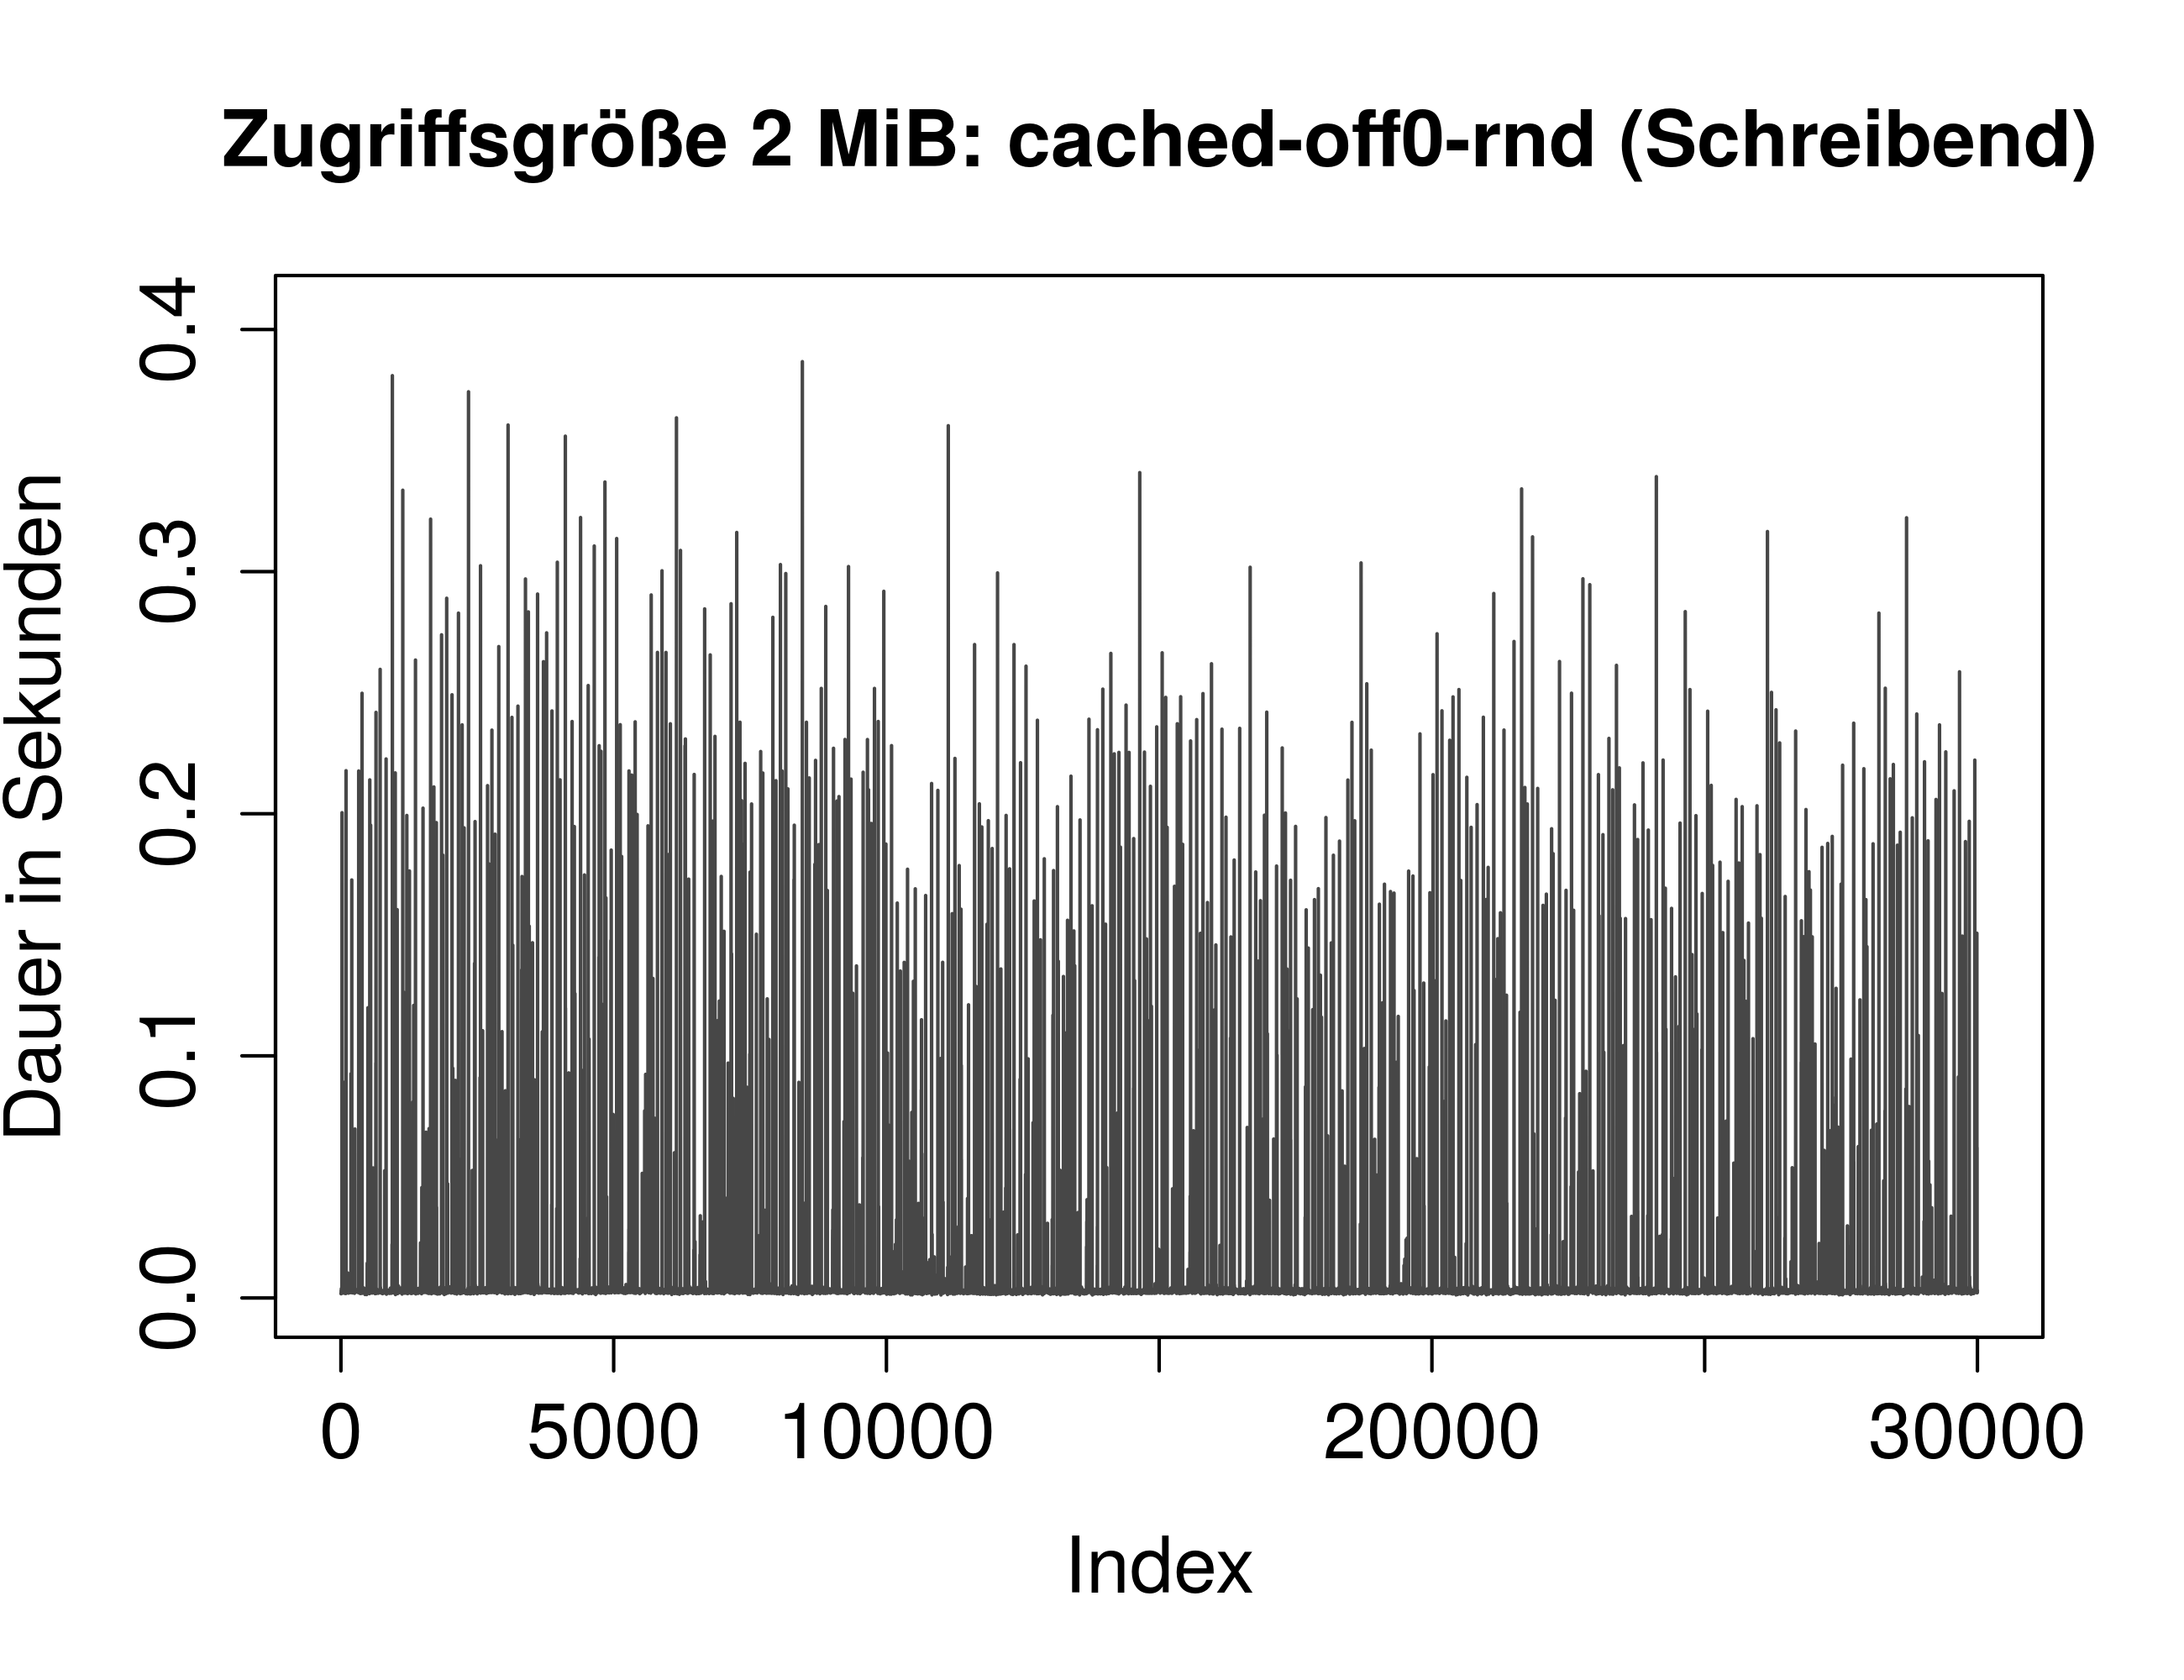
\includegraphics[width=.43\textwidth]{Bilder/Plots/exploration/plot_Size2097152_write_rnd.png}
	}		
	\caption{Detailbetrachtung aller Messungen mit Zugriffsgröße 2097152KB}
	\label{fig:groesse2097152}
\end{figure} 


Um die Messdaten noch detaillierter darzustellen, müssen kleine Ausschnitte herausgegriffen werden. Zunächst betrachte ich die ersten $250$ Messungen. \ref{fig:first250}
Auf den ersten Blick scheint bei cached-off0-seq-W eine gewisse Periodizität ersichtlich (etwa alle 45 Messungen gibt es einen größeren Sprung, alternierend sind die Laufzeiten jeweils etwas langsamer und schneller). Nach genau $123$ Punkten scheint sich das Muster zu wiederholen, dort befindet sich der zweitgrößte Messwert. Wenn man nun als erstes simples Modell eine Fortführung der augenscheinlichen Periodizität der ersten $123$ Messpunkten betrachtet, so erkannt man doch, dass der Verlauf recht unregelmäßig ist. \ref{fig:periodicity} \\
Bei den anderen Graphen kann keine so simple Periodizität vermutet werden.

\begin{figure}
	\subfloat{
		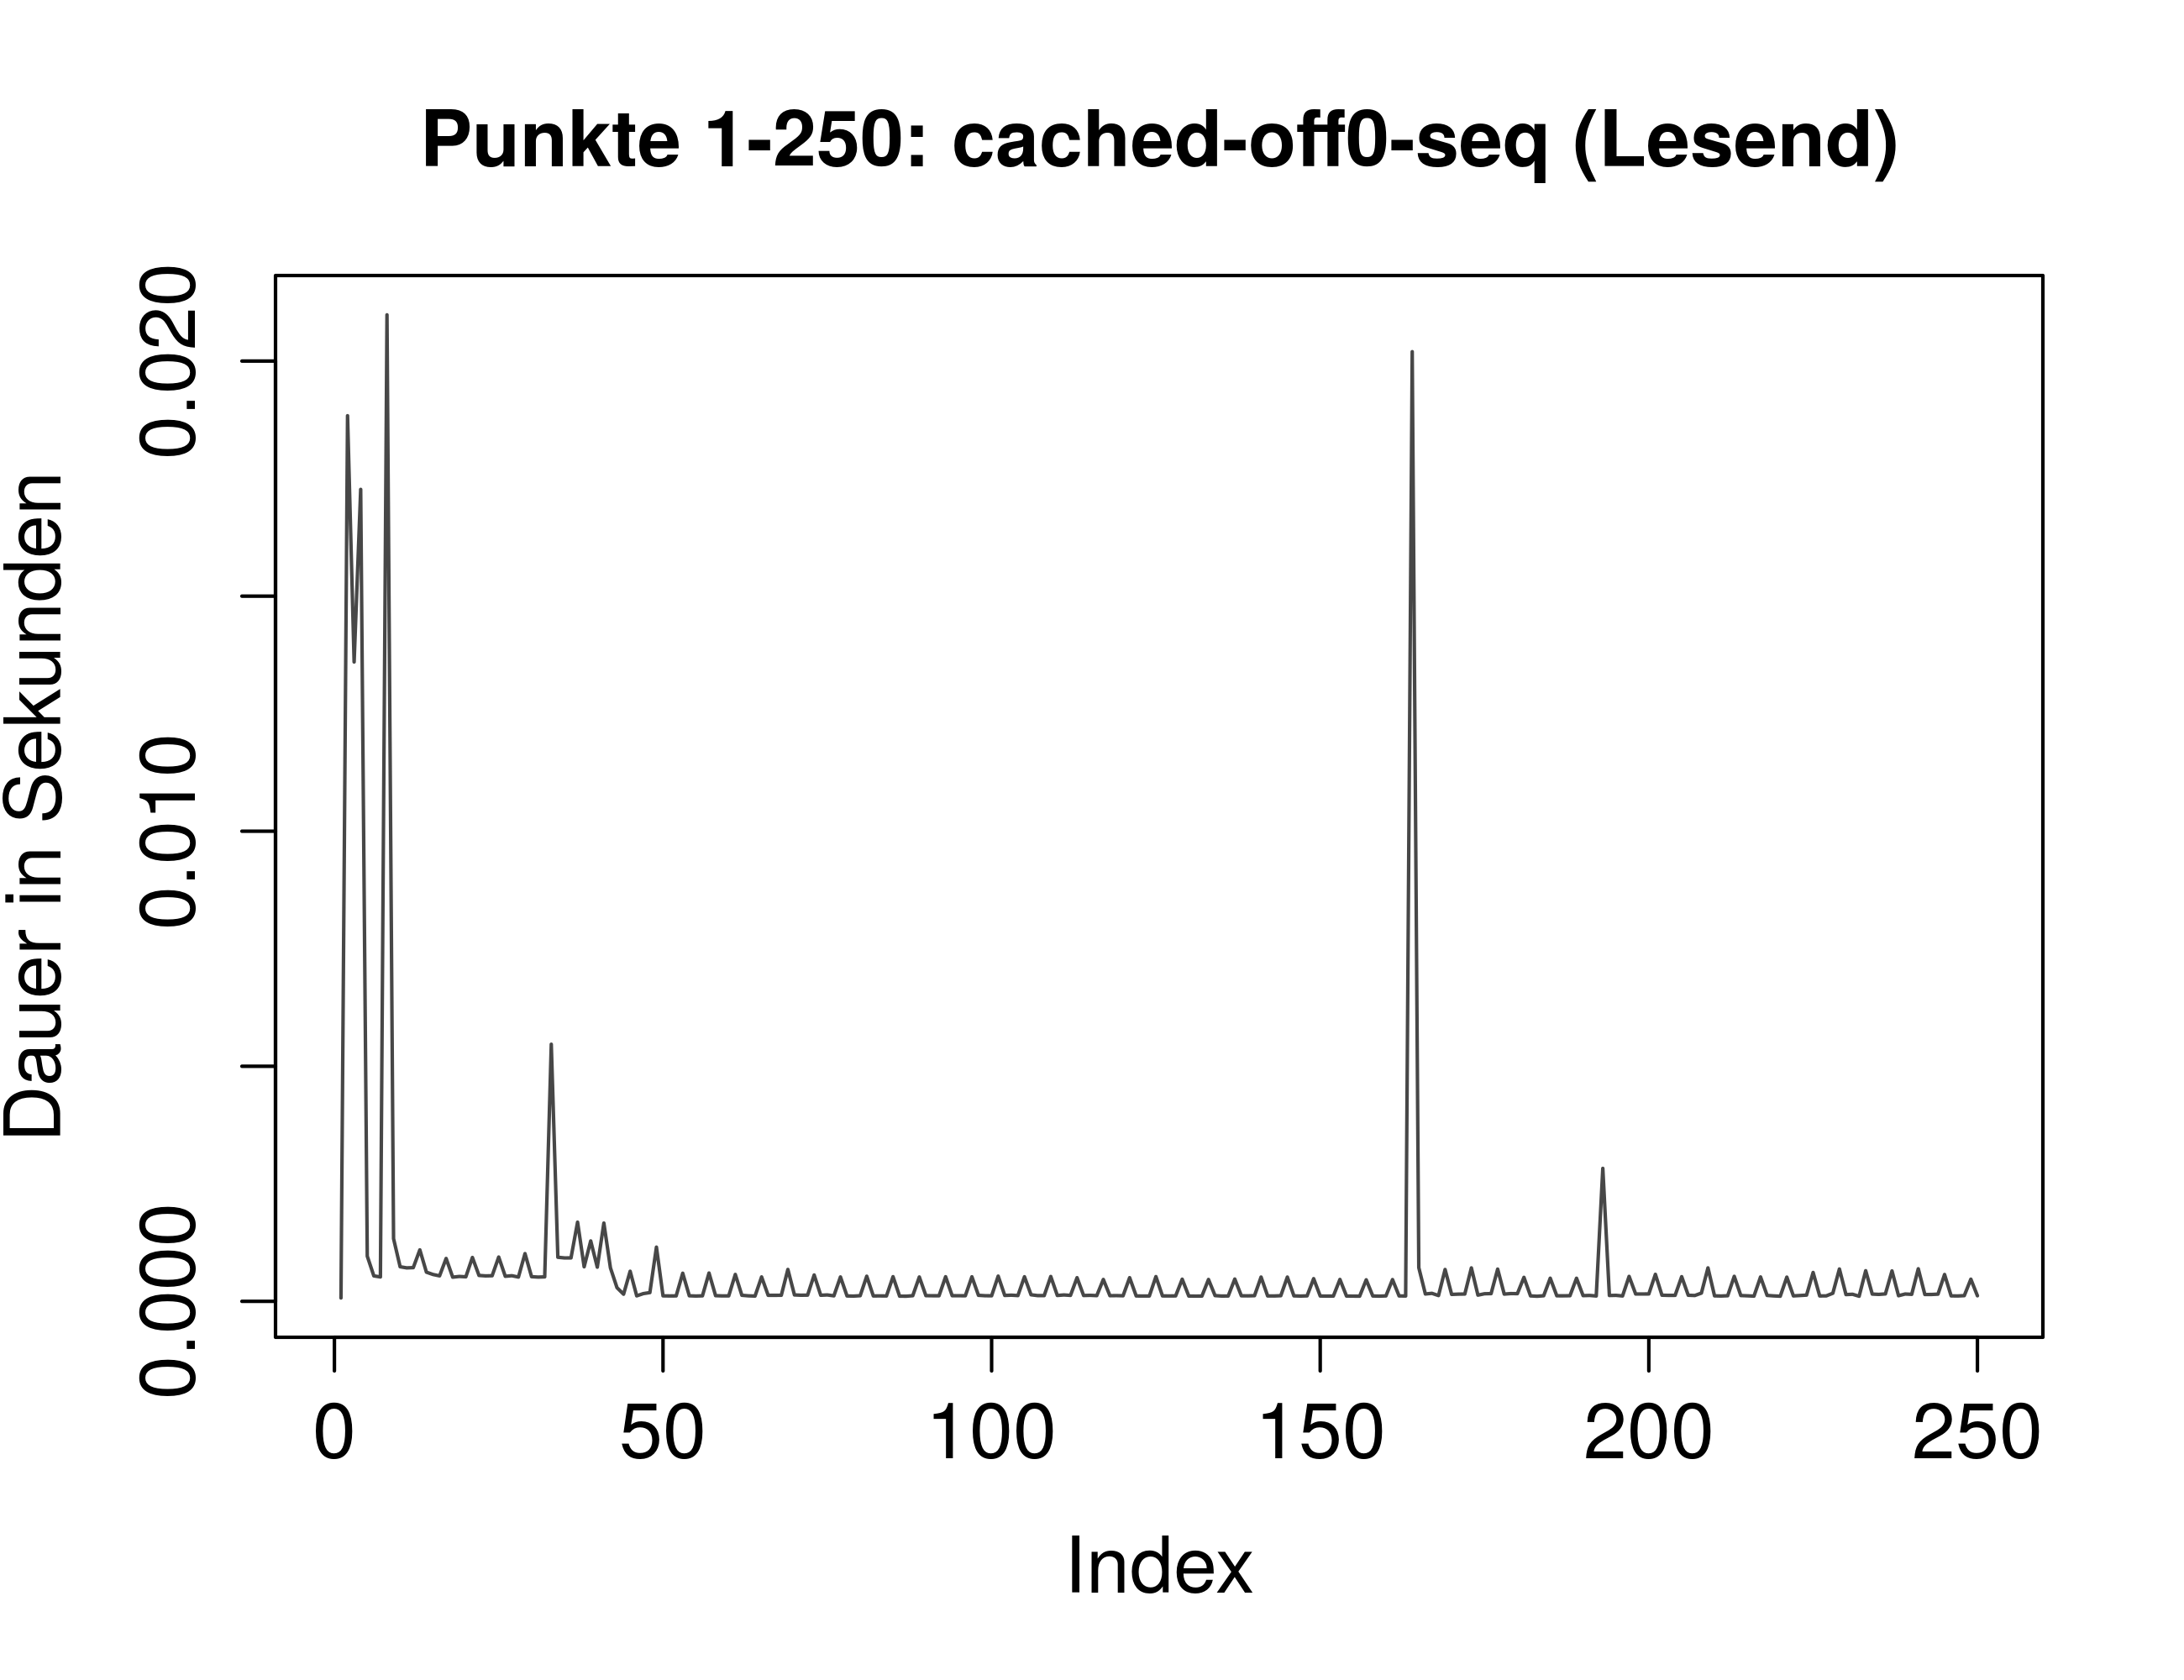
\includegraphics[width=.43\textwidth]{Bilder/Plots/exploration/plot_First250_read_seq.png}
	}
	\hfill
	\subfloat{
		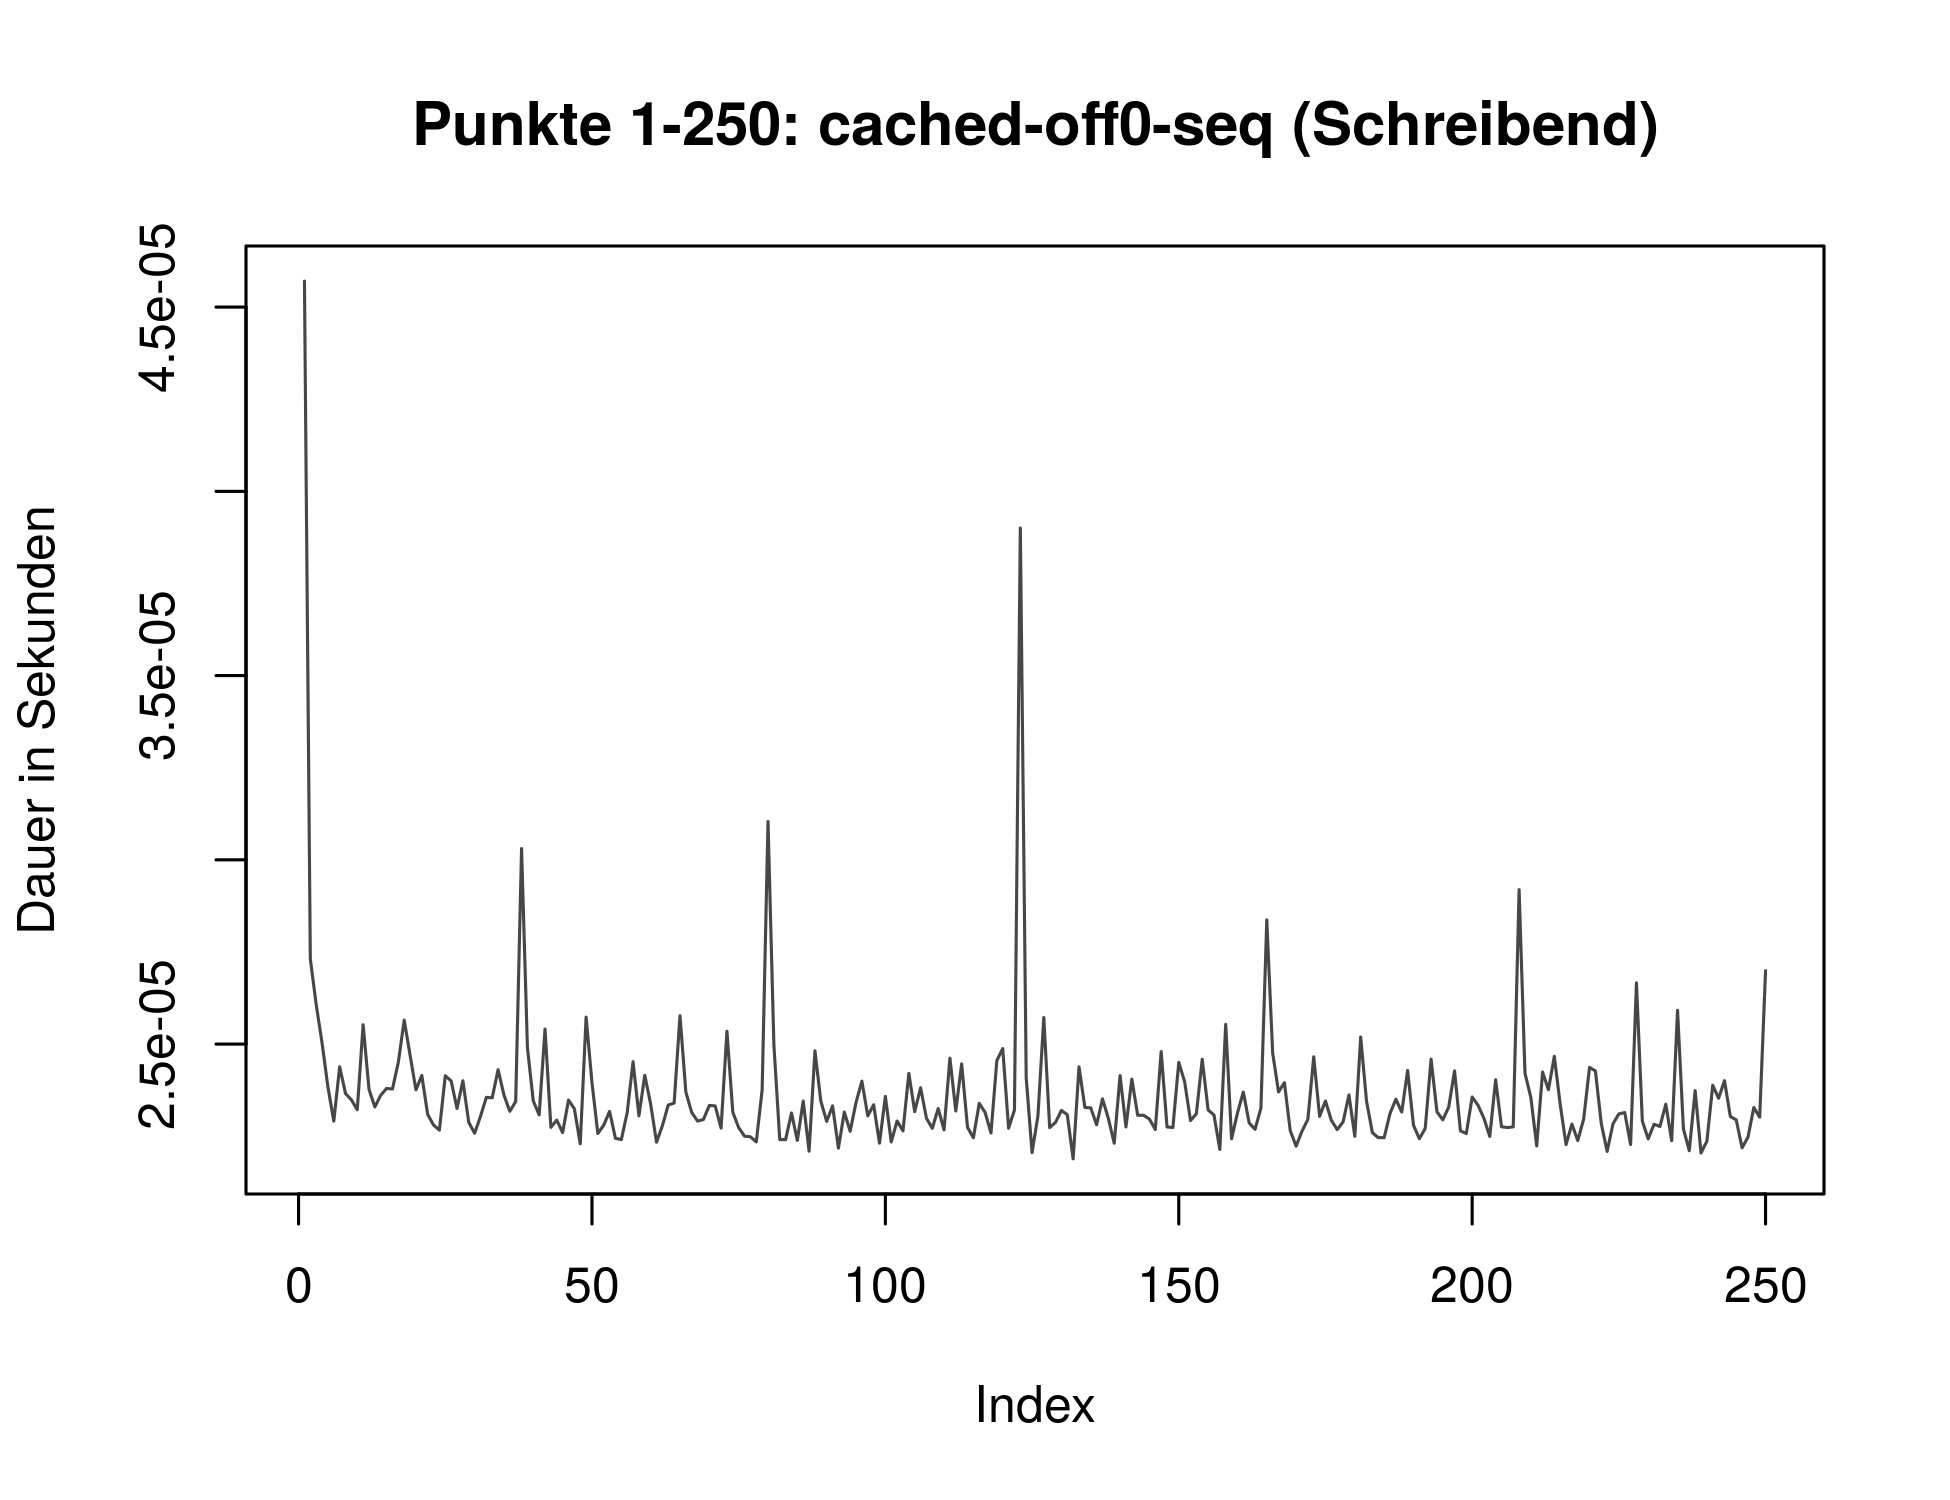
\includegraphics[width=.43\textwidth]{Bilder/Plots/exploration/plot_First250_write_seq.png}
	}\\
	\subfloat{
		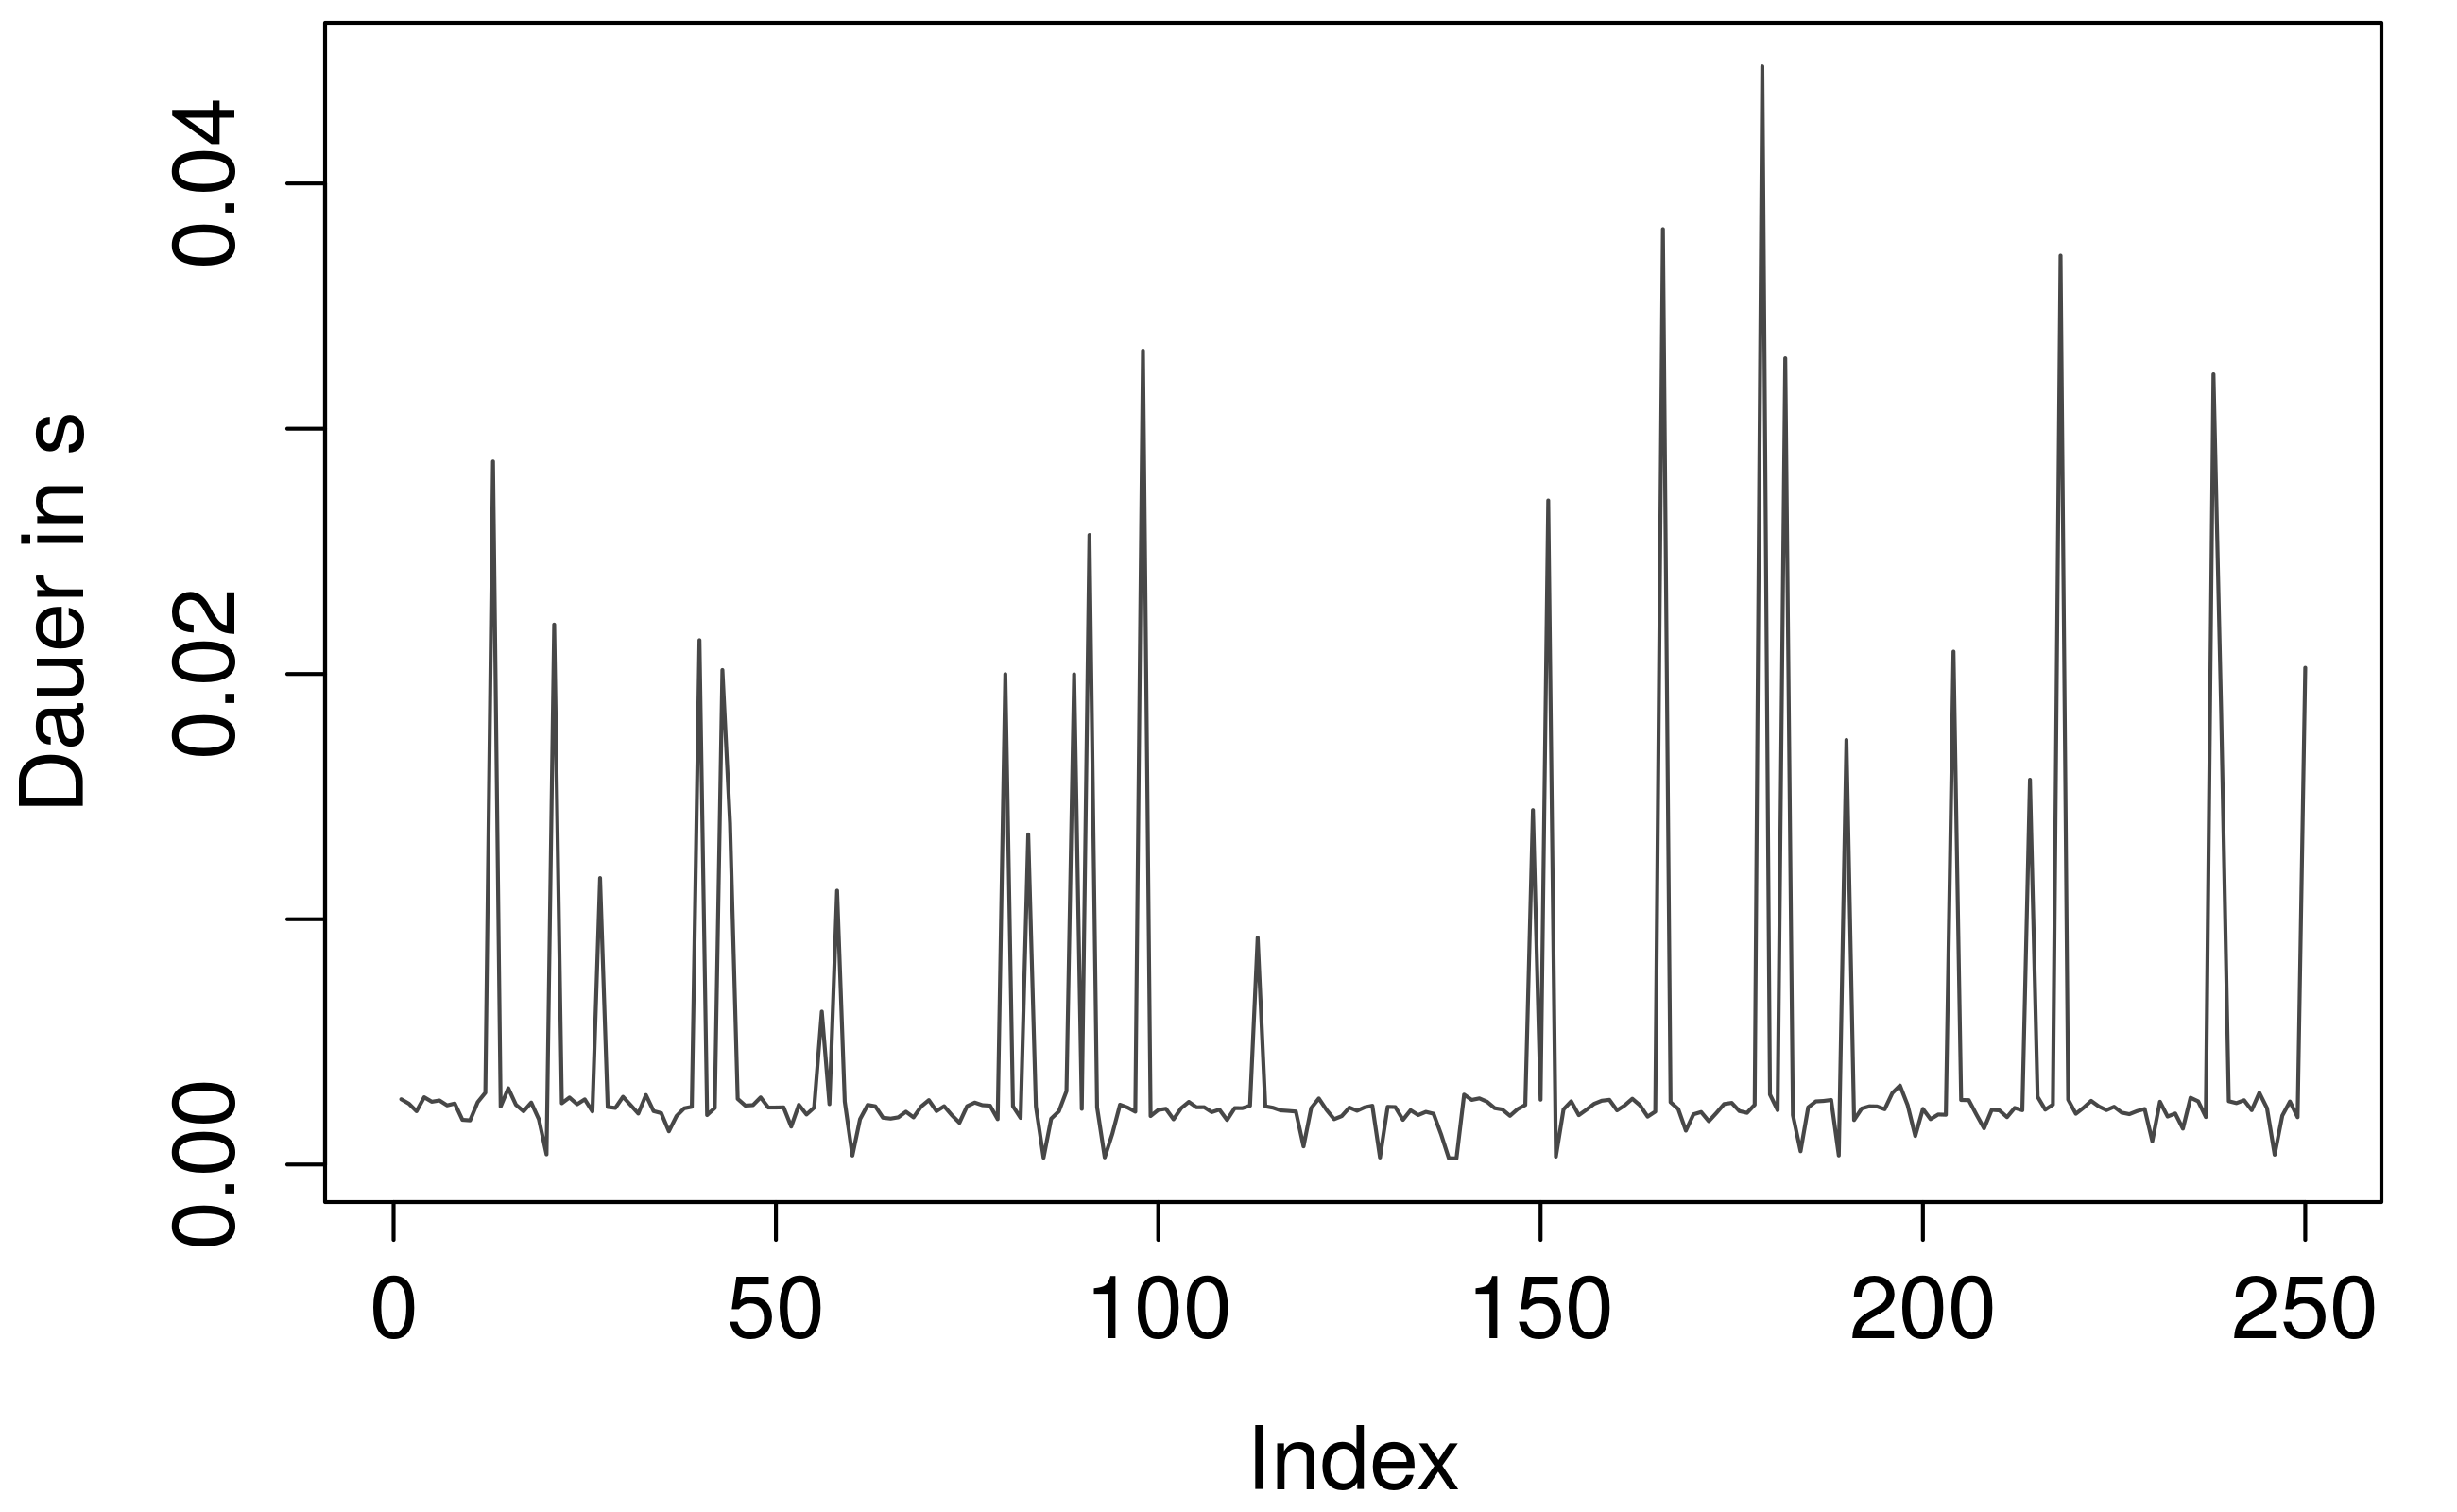
\includegraphics[width=.43\textwidth]{Bilder/Plots/exploration/plot_First250_read_rnd.png}
	}
	\hfill
	\subfloat{
		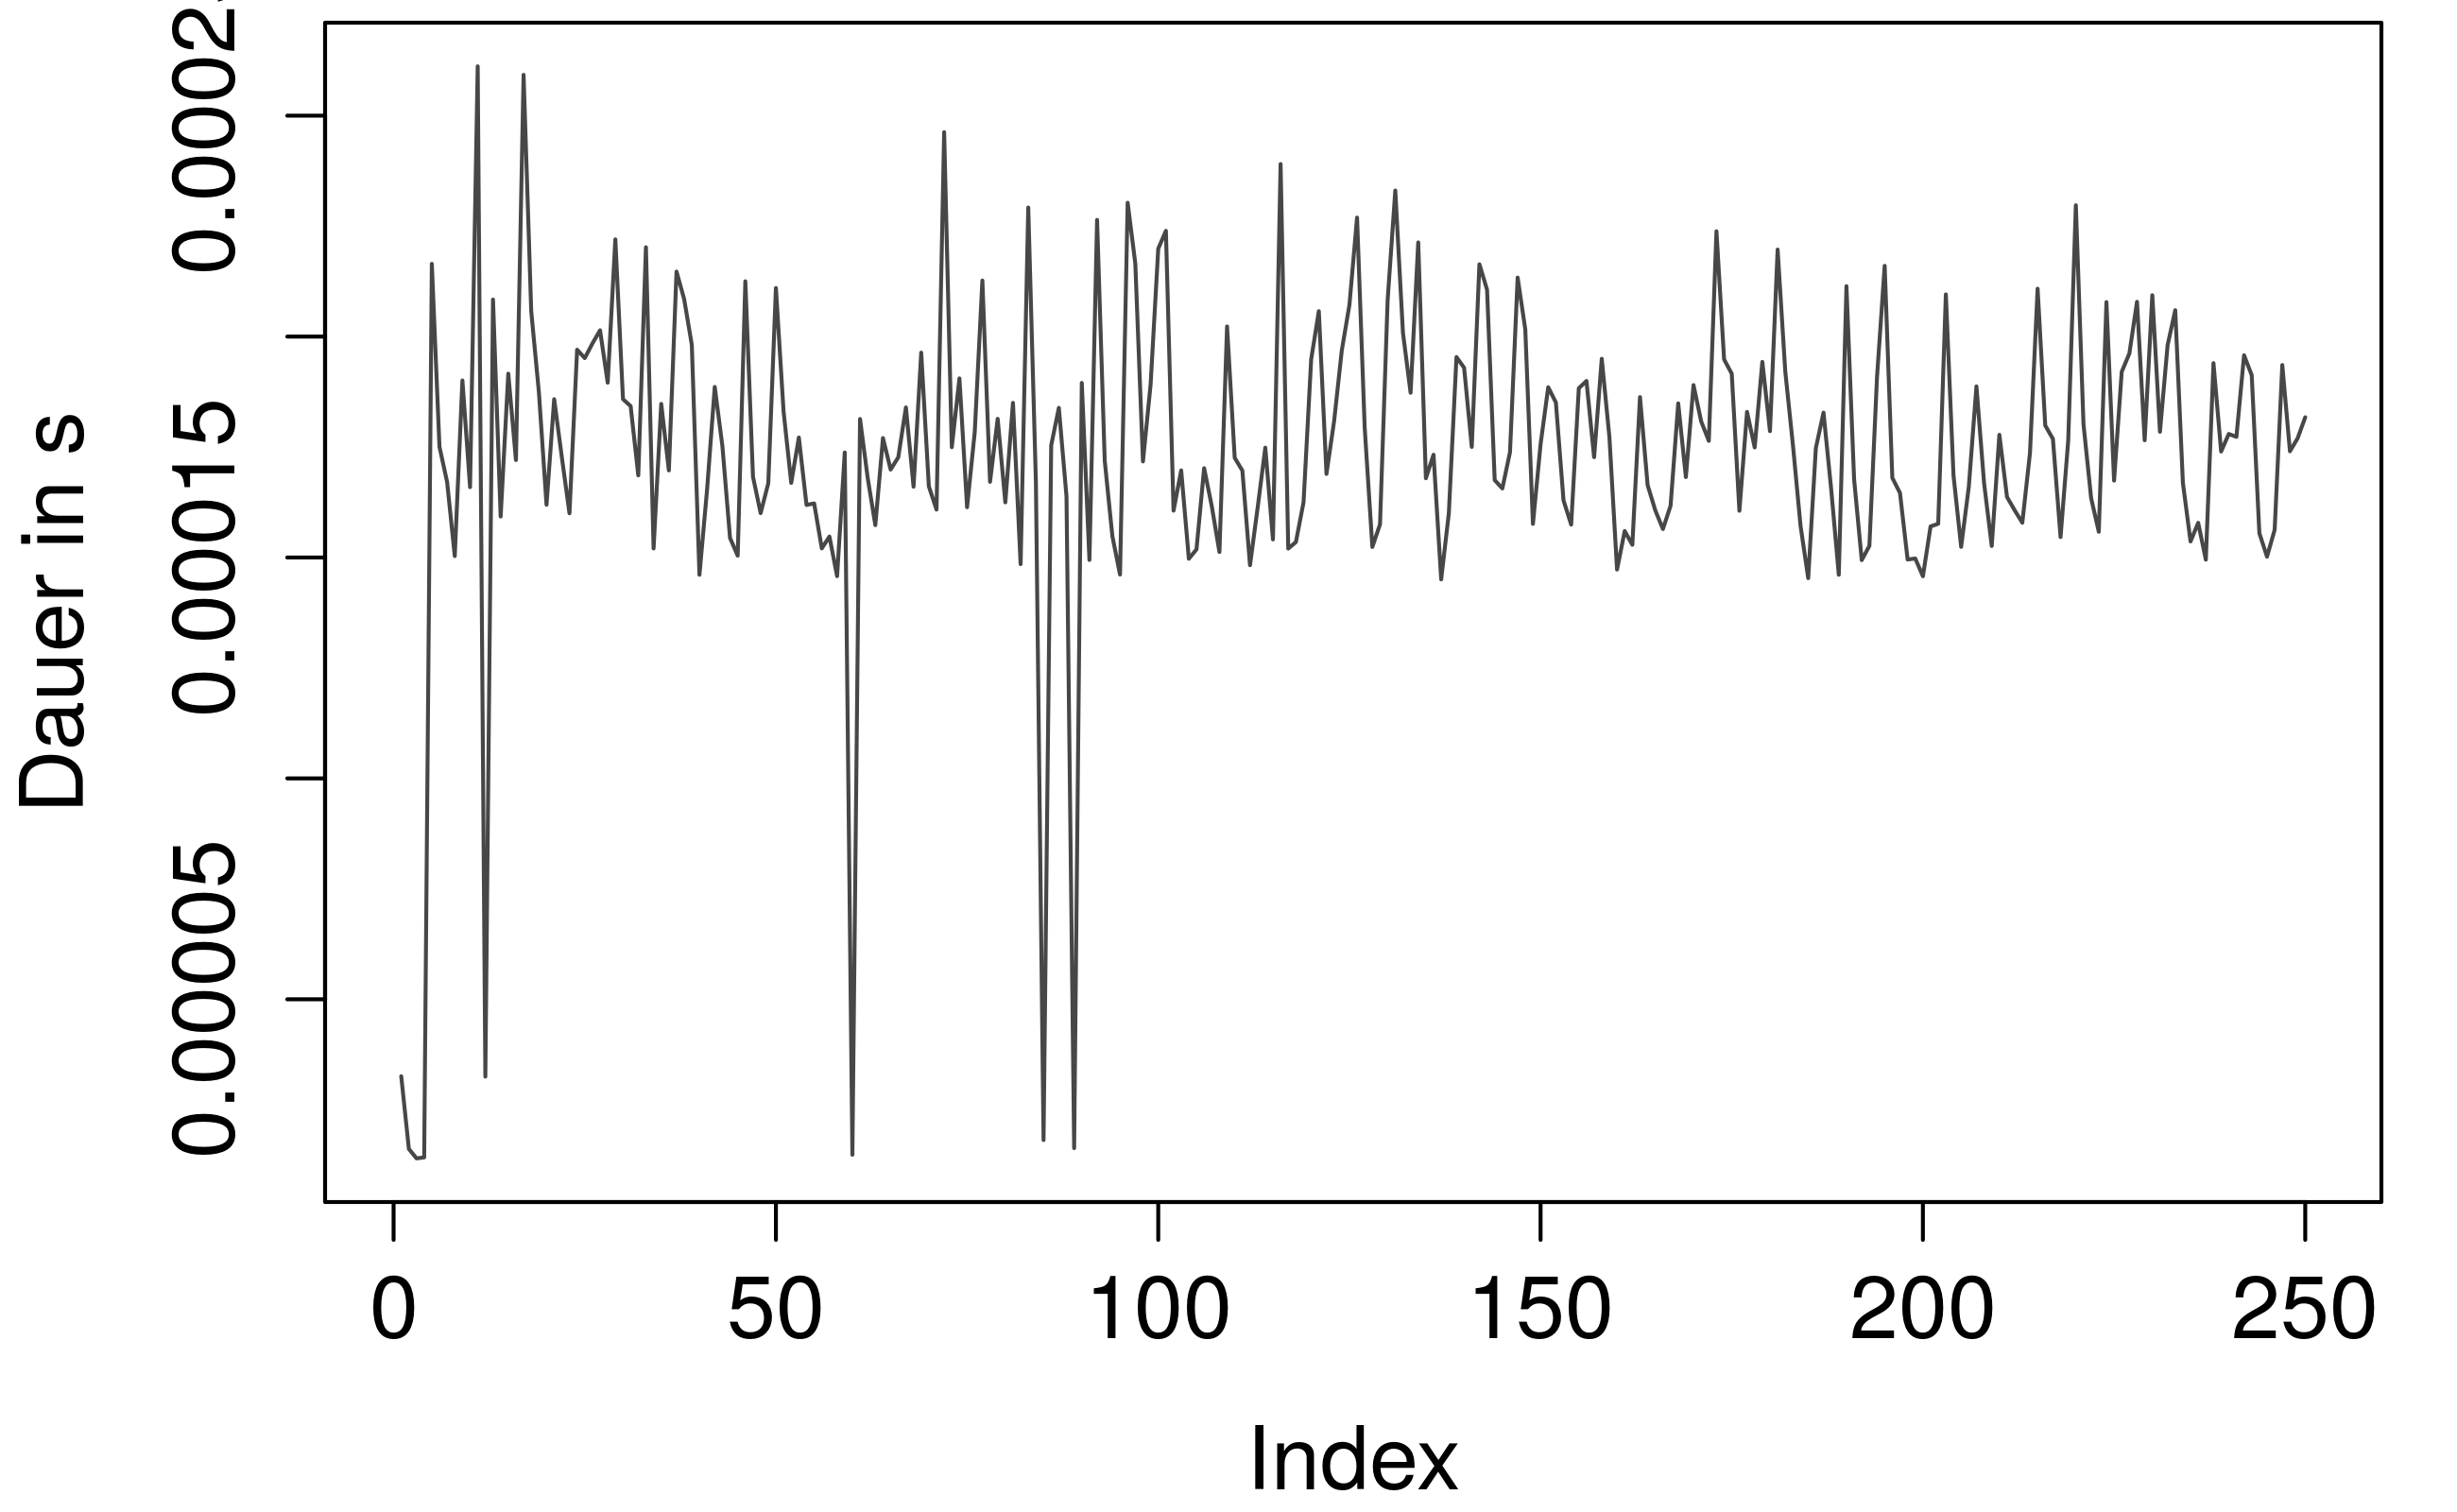
\includegraphics[width=.43\textwidth]{Bilder/Plots/exploration/plot_First250_write_rnd.png}
	}		
	\caption{Detailbetrachtung der ersten 250 Messungen}
	\label{fig:first250}
\end{figure} 

\begin{figure}
	\subfloat{
		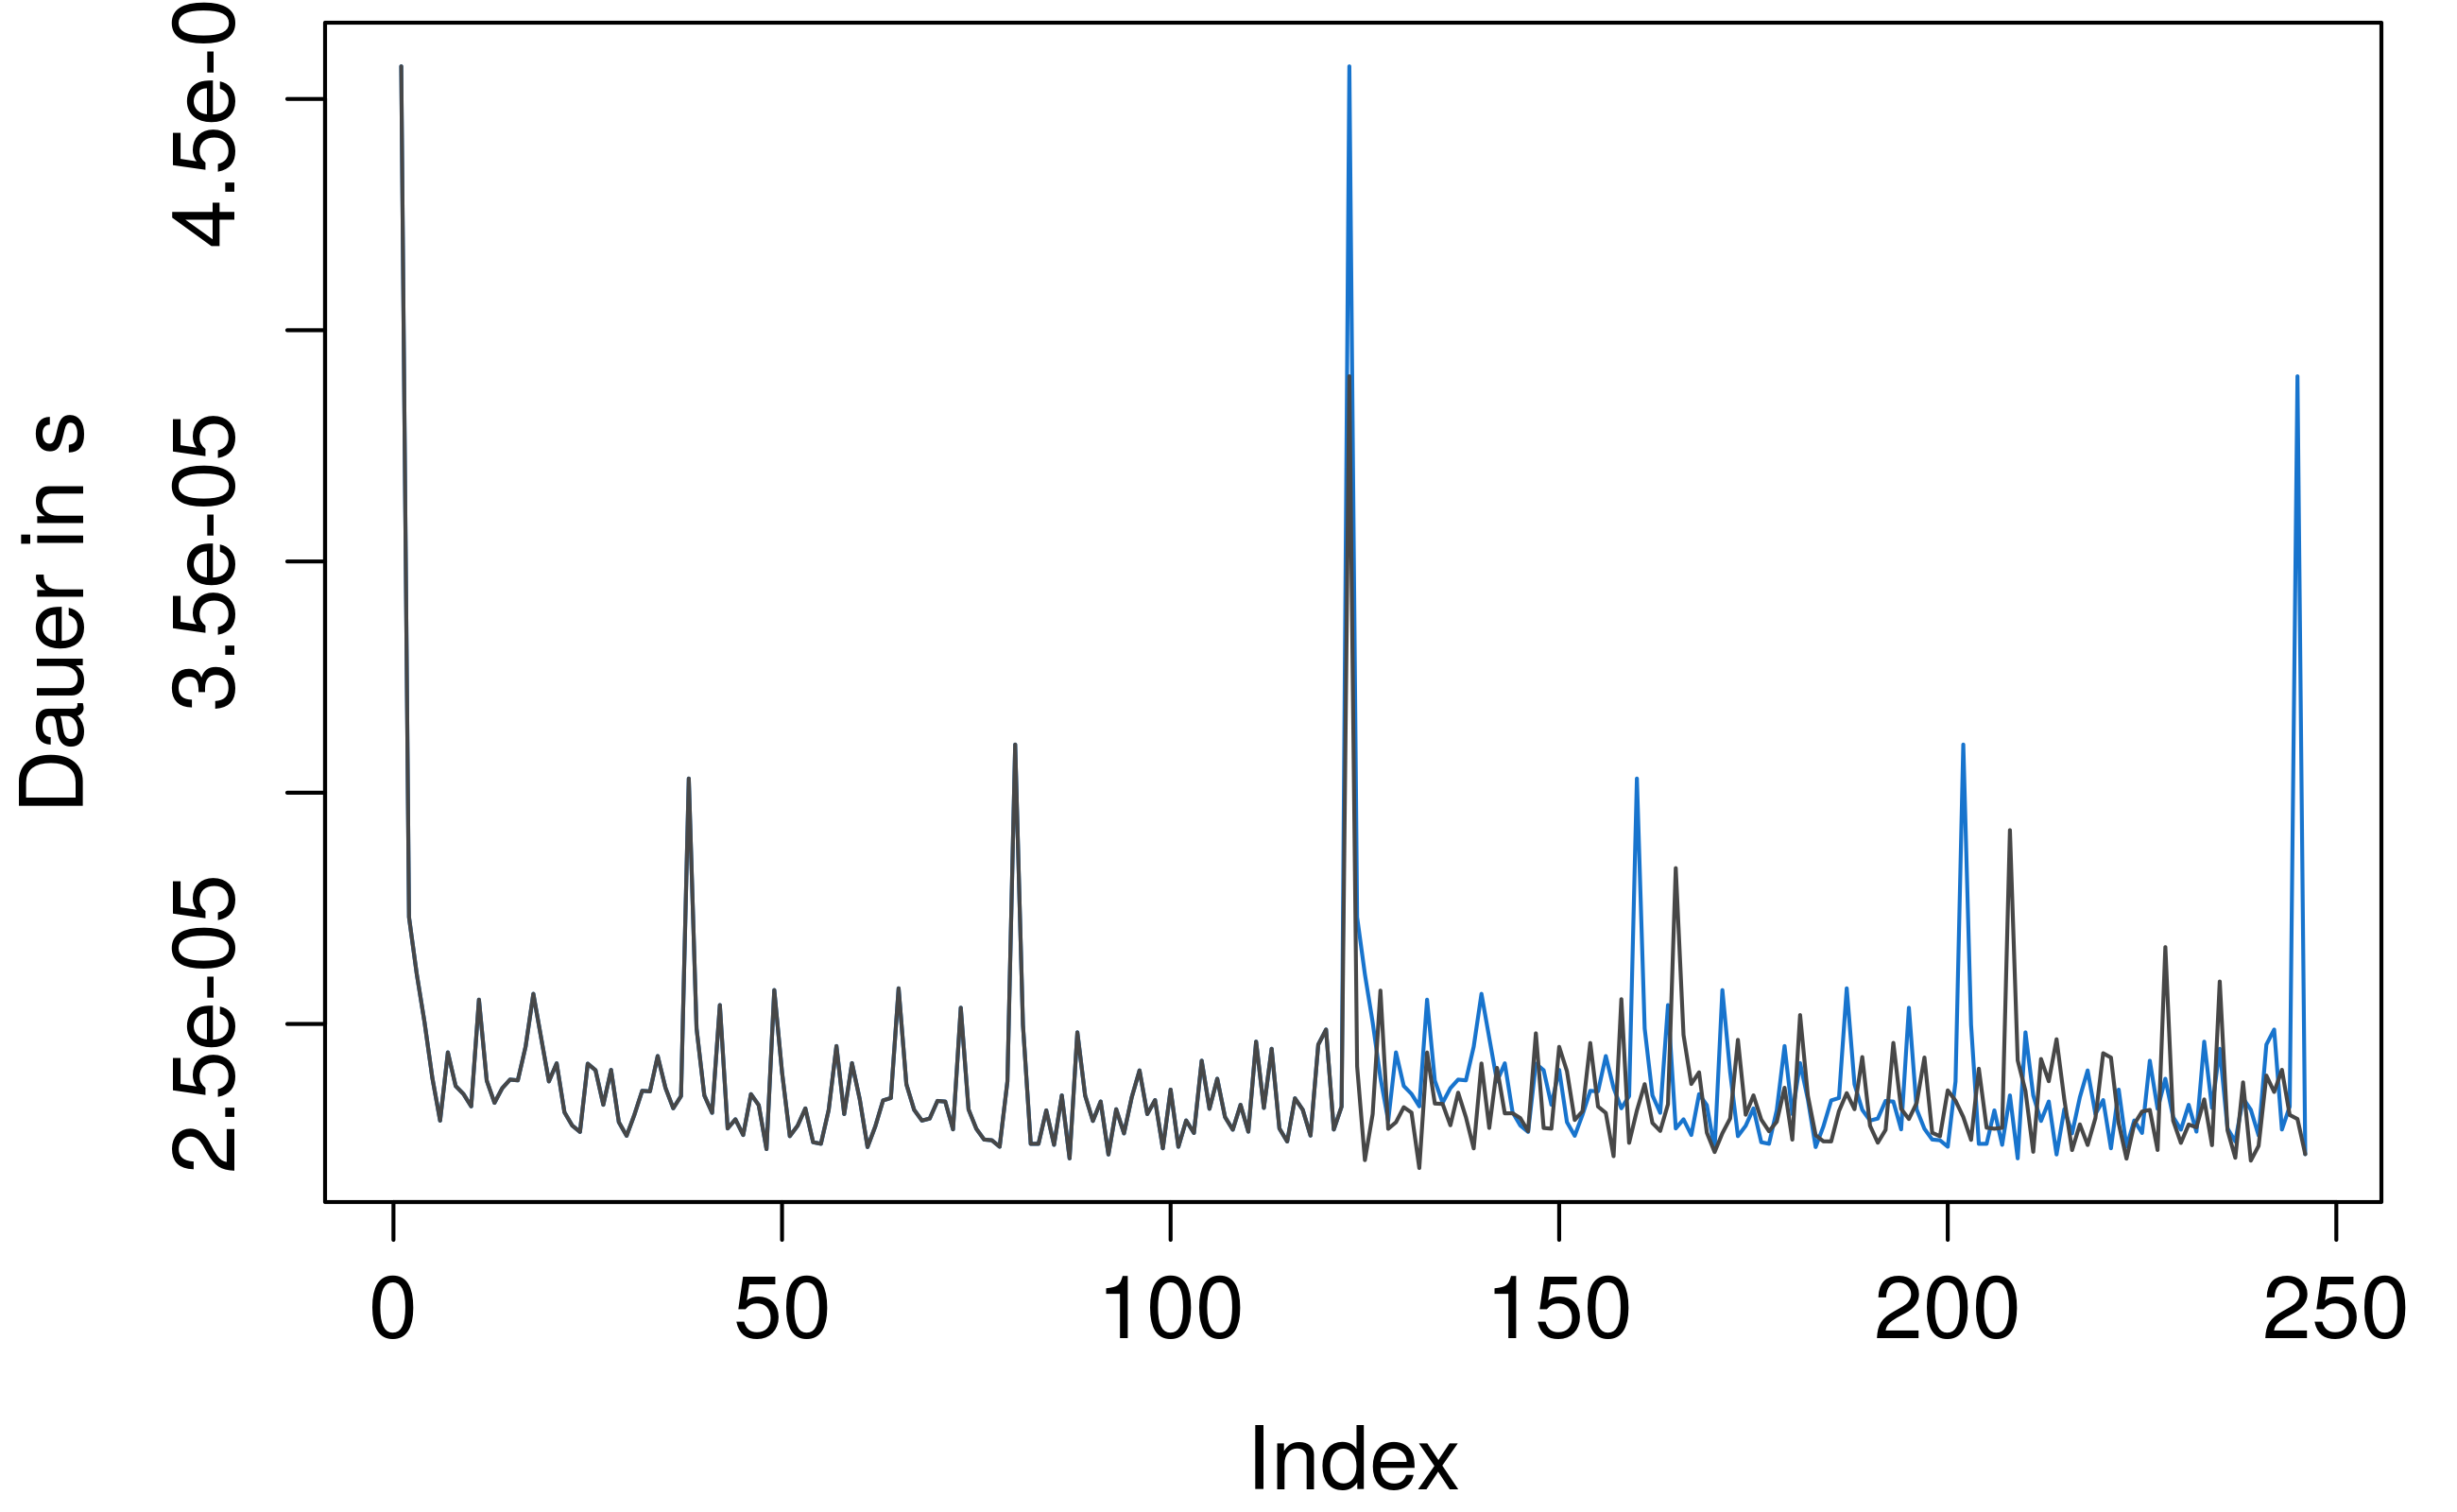
\includegraphics[width=.8\textwidth]{Bilder/Plots/exploration/plot_periodicitywrite_seq.png}
	}	
	\caption{Wiederholung der ersten Werte, als erstes einfaches Modell}
	\label{fig:periodicity}
\end{figure} 

Eine weitere Detailbetrachtung mache ich bei den Messungen 30.001 bis 30.250. \ref{fig:from100001}\\
Hier scheint eine Periodizität bei cached-off0-seq-R vorhanden zu sein. Und wenn eine Überlappung wie zuvor durchgeführt wird (diesmal nach den ersten 129 Messungen), so erkennt man, dass dieses simple Modell die Ausreißer für diesen kleinen Ausschnitt exakt vorhersagen kann. \ref{fig:periodicity100001}\\
Im Allgemeinen kann dies jedoch offensichtlich nicht funktionieren. Doch unsere Annahme \textbf{ABSCHNITT} einer gewissen Periodizität in der Leistung des E/A-Systems ist scheinbar gerechtfertigt. Ein Modell das versucht diese auszunutzen muss eine komplexere Methode als schlichtes Übertragen vorheriger Leistungswerte haben, ansonsten kann es wohl nur in äußerst eingeschränktem Maße korrekte Leistung vorhersagen.

\begin{figure}
	\subfloat{
		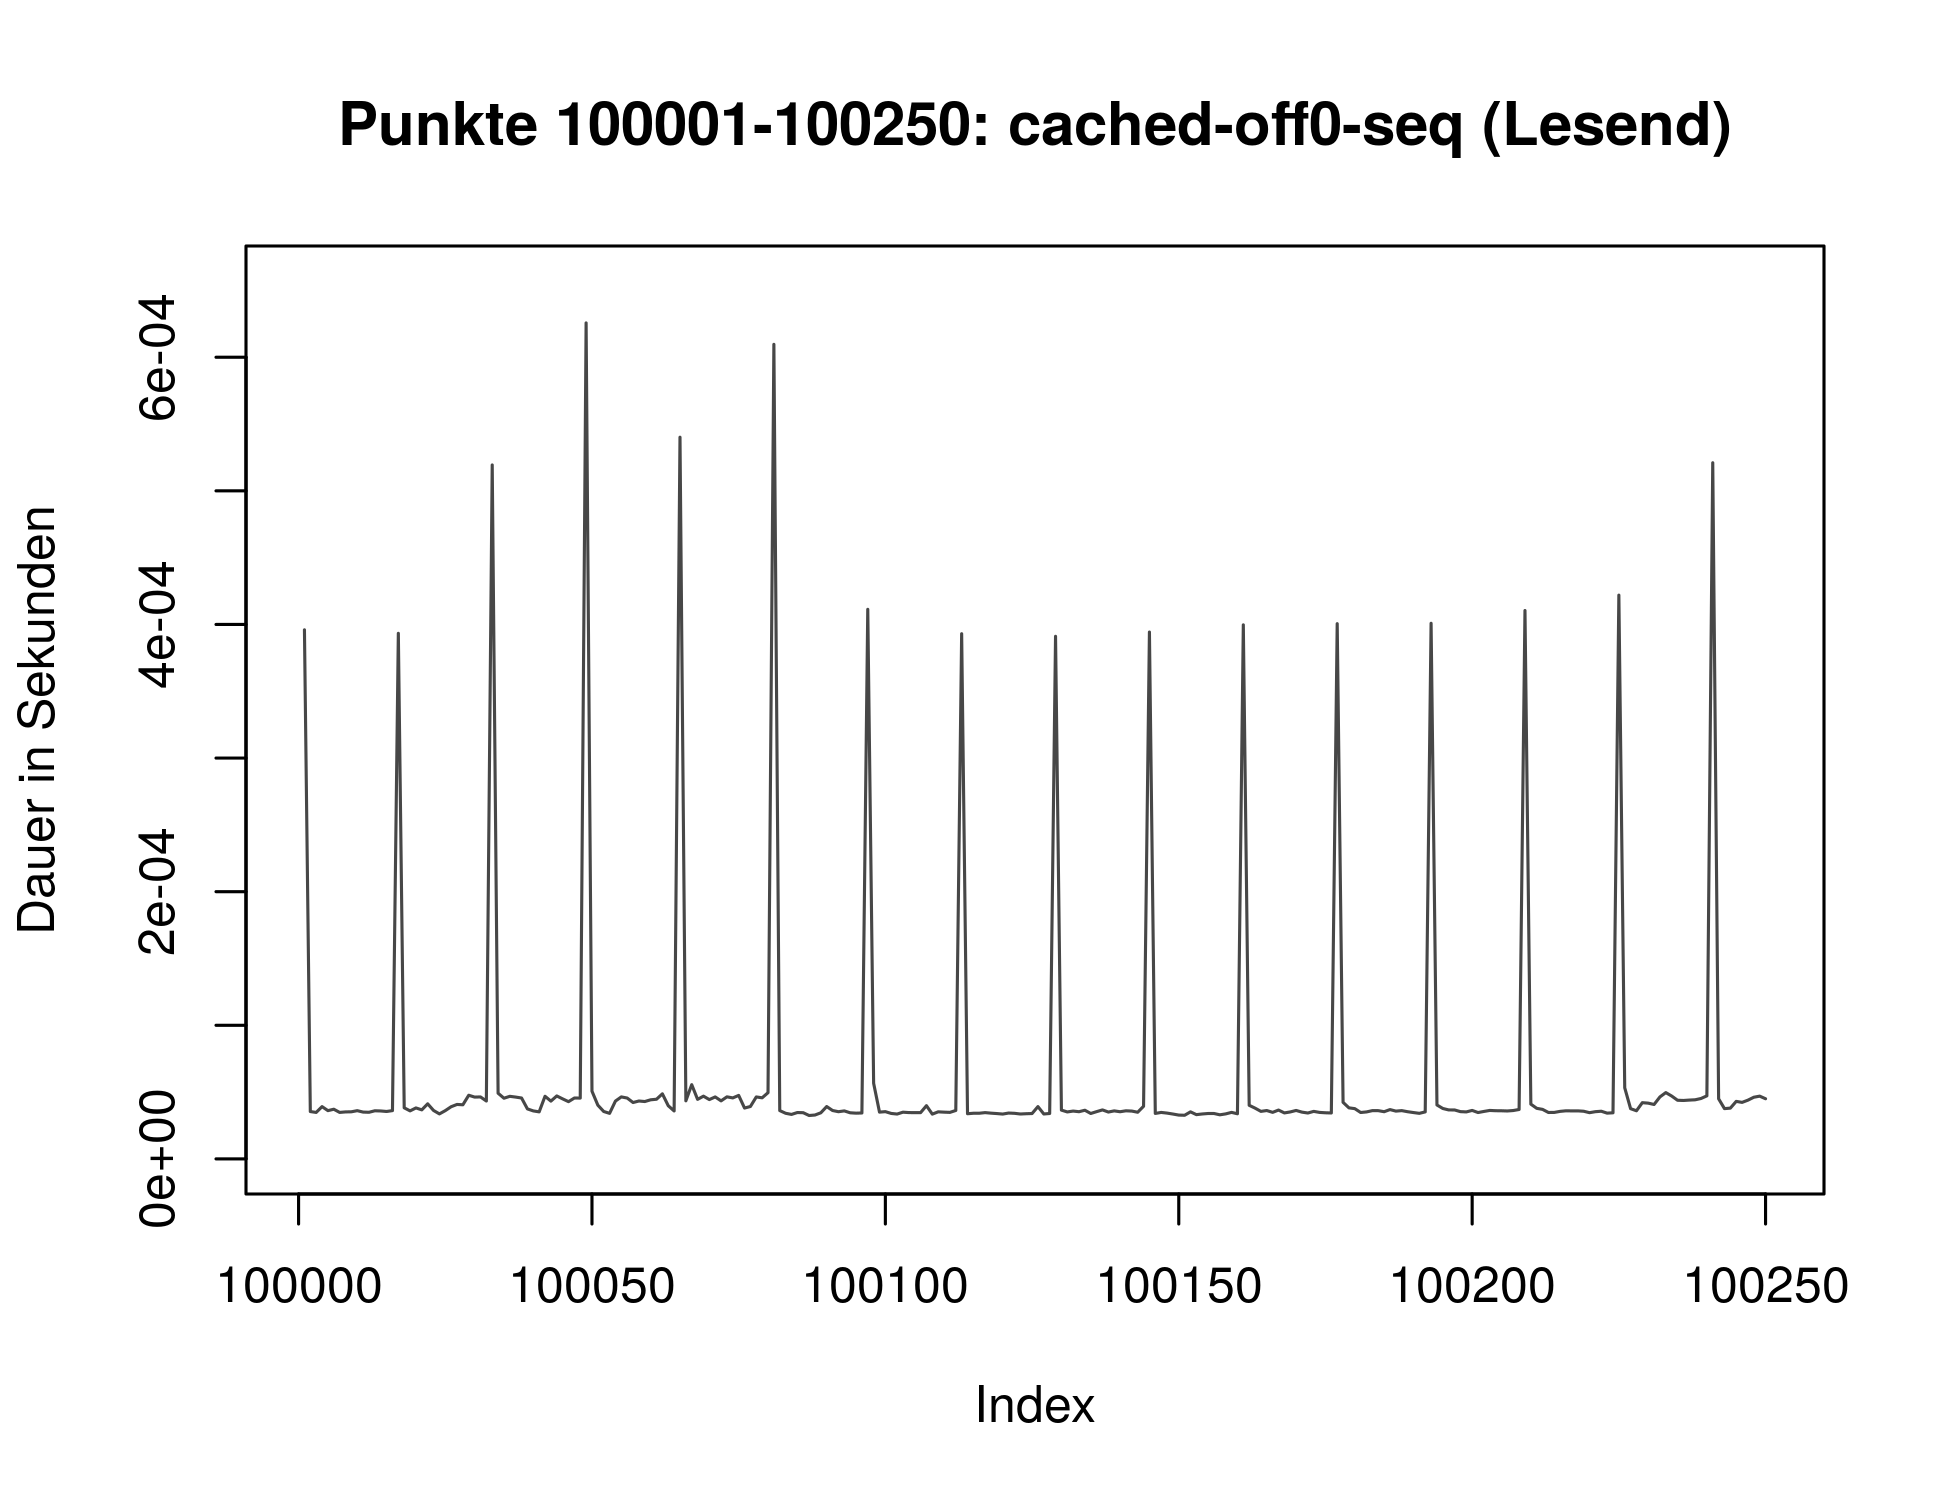
\includegraphics[width=.43\textwidth]{Bilder/Plots/exploration/plot_From100001to100250_read_seq.png}
	}
	\hfill
	\subfloat{
		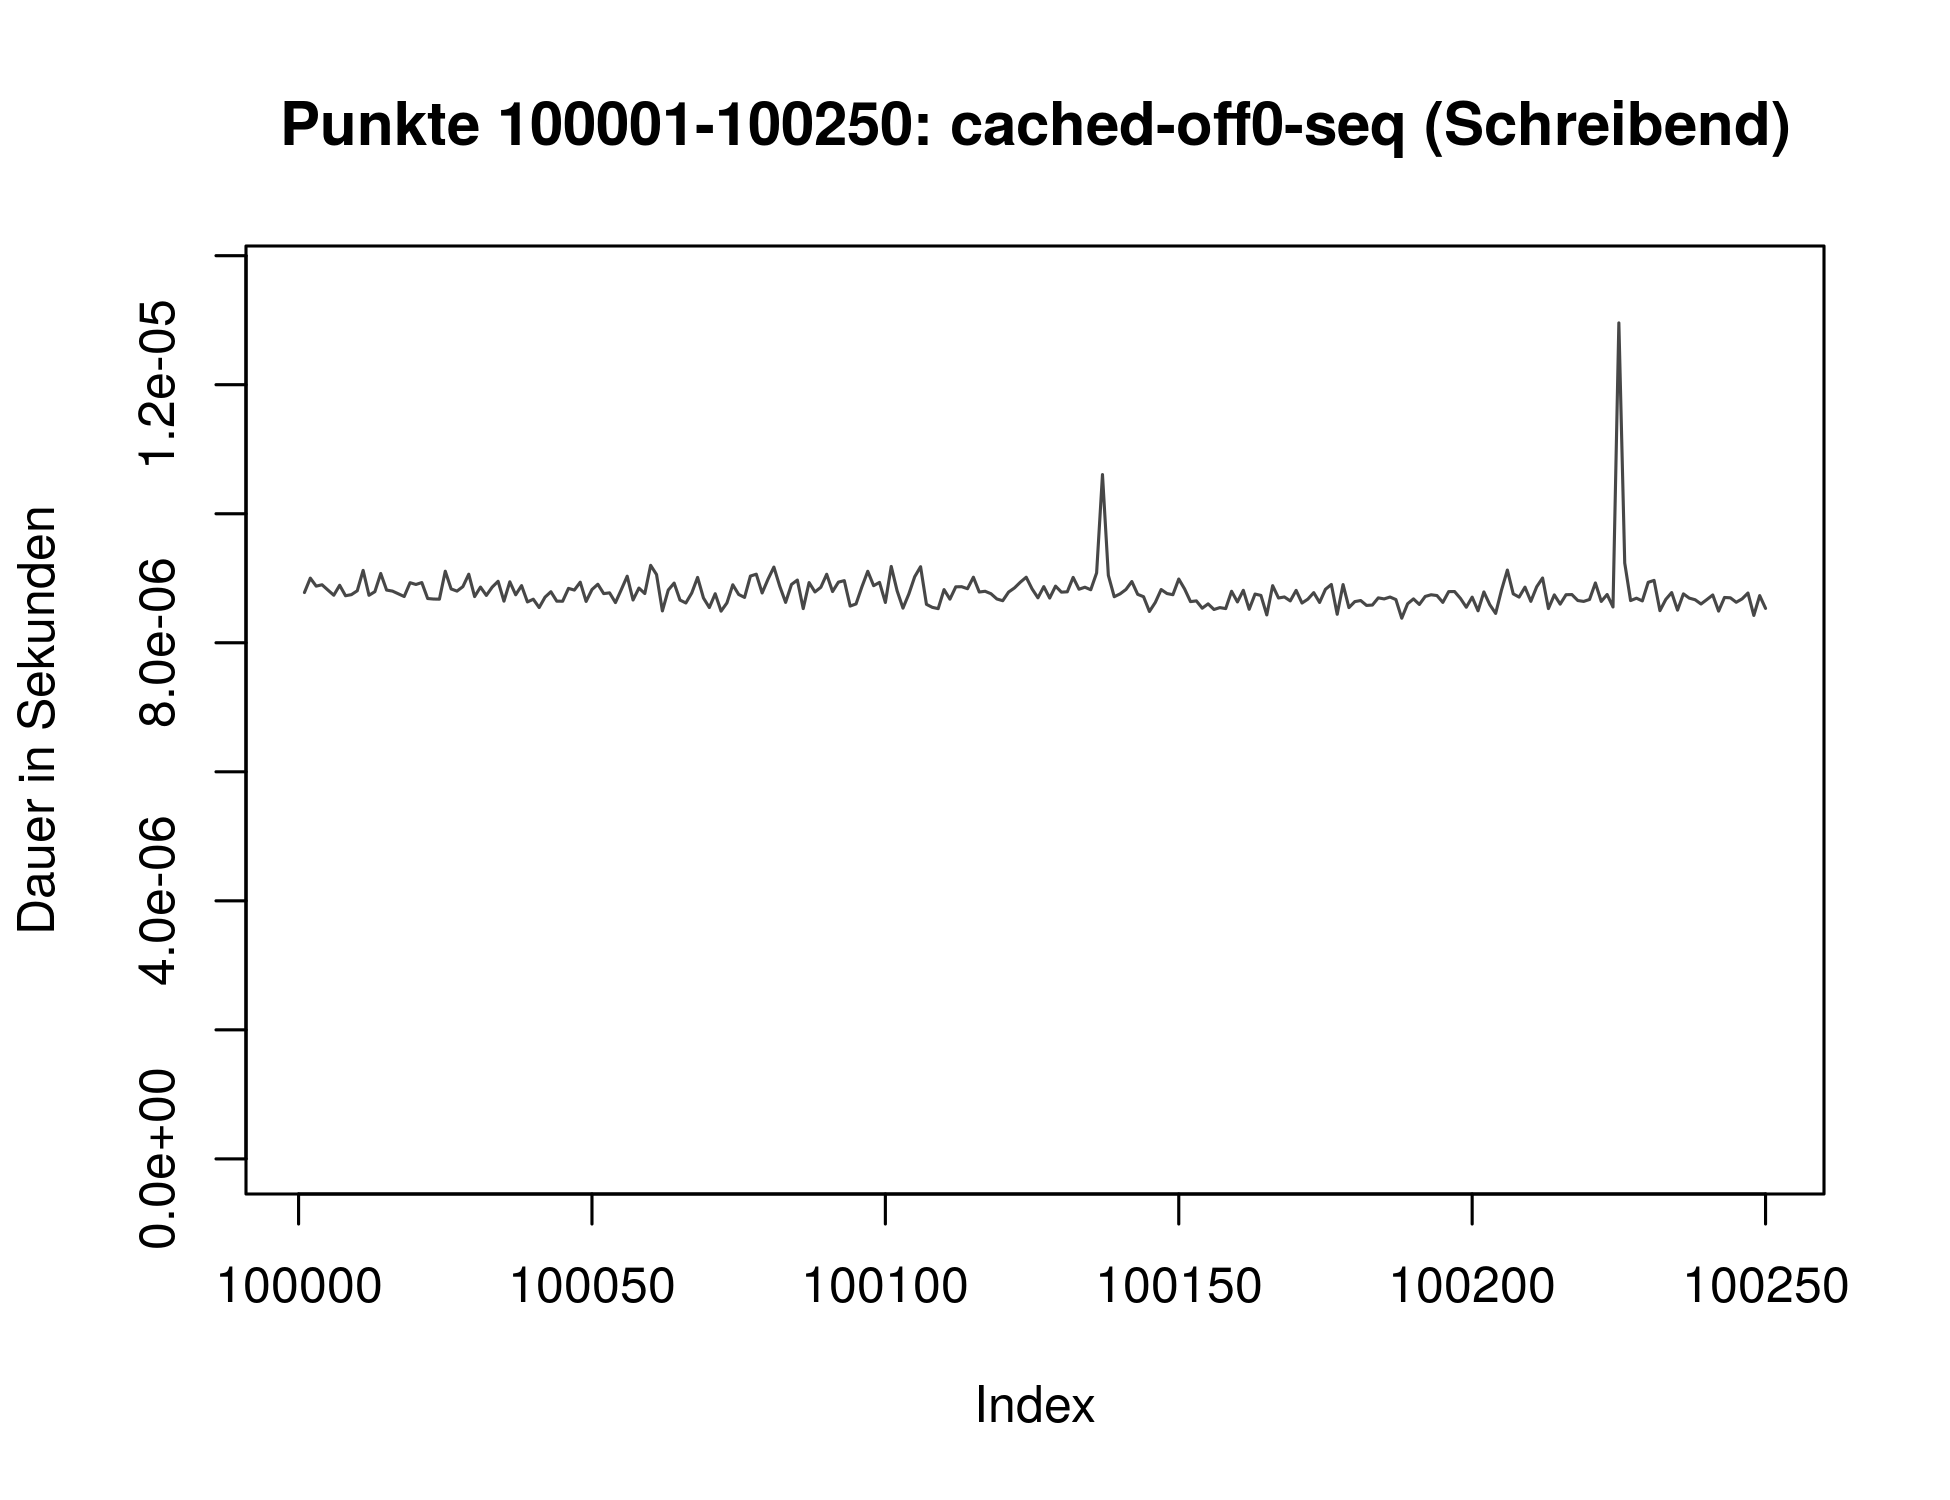
\includegraphics[width=.43\textwidth]{Bilder/Plots/exploration/plot_From100001to100250_write_seq.png}
	}\\
	\subfloat{
		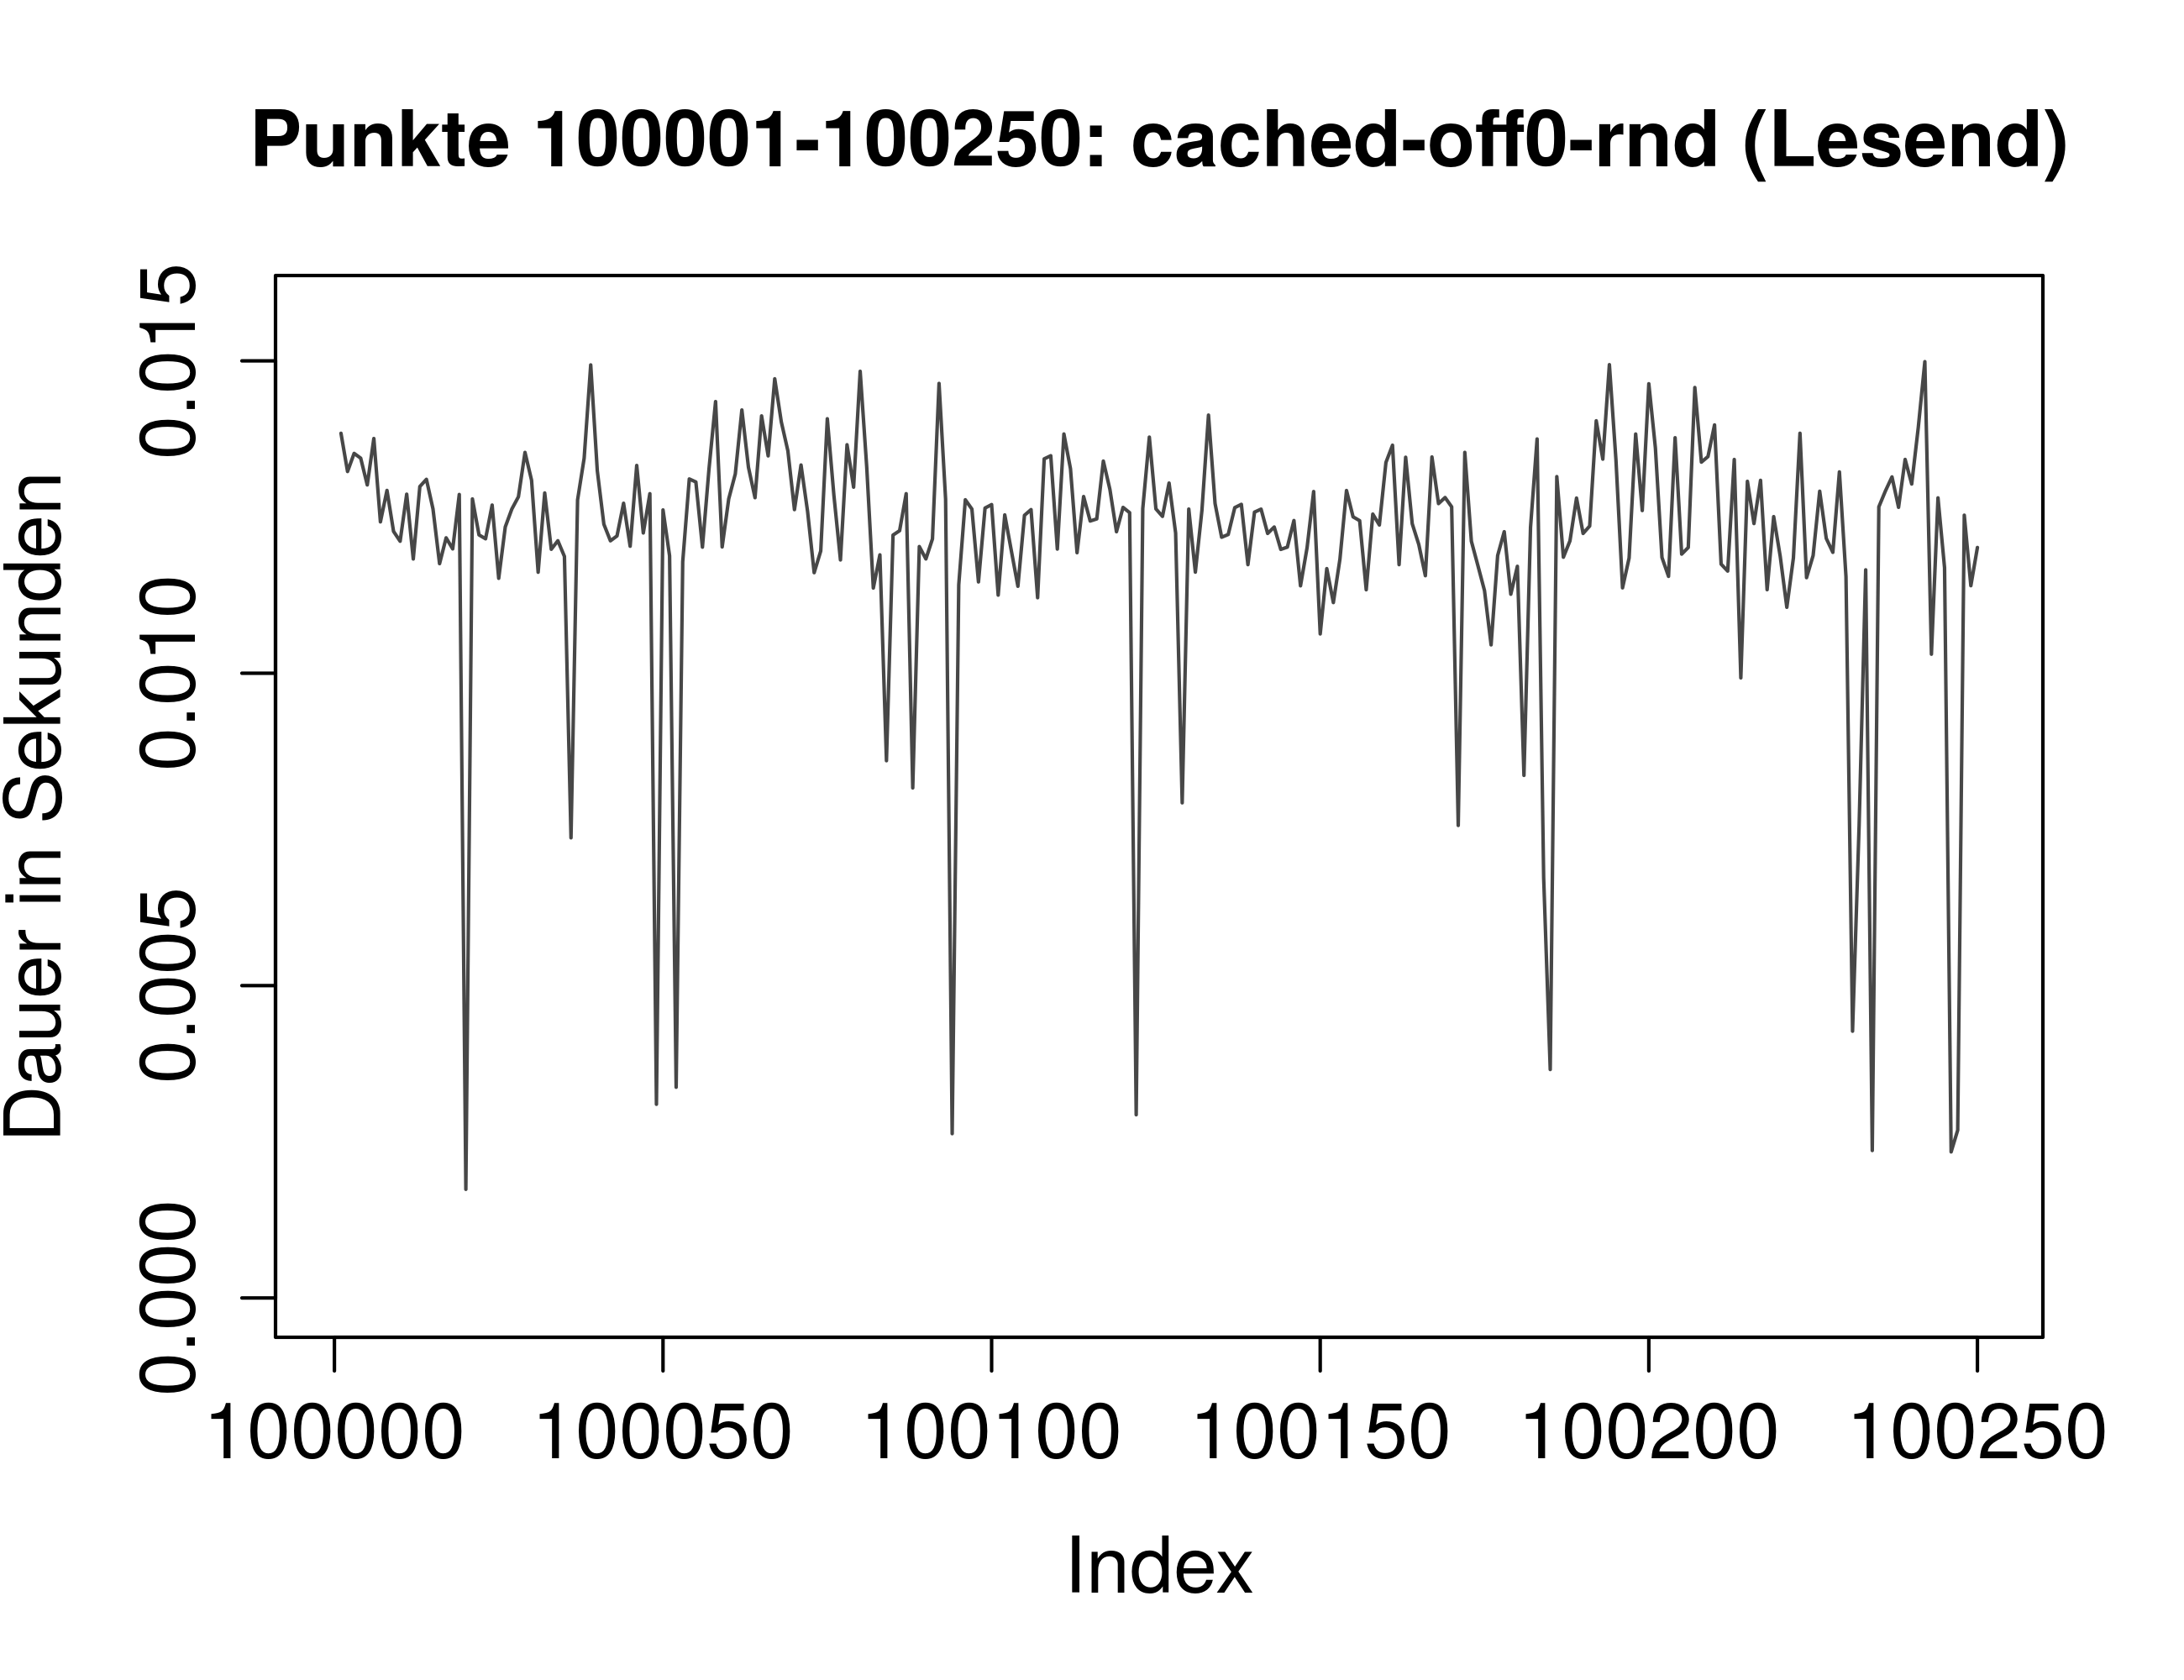
\includegraphics[width=.43\textwidth]{Bilder/Plots/exploration/plot_From100001to100250_read_rnd.png}
	}
	\hfill
	\subfloat{
		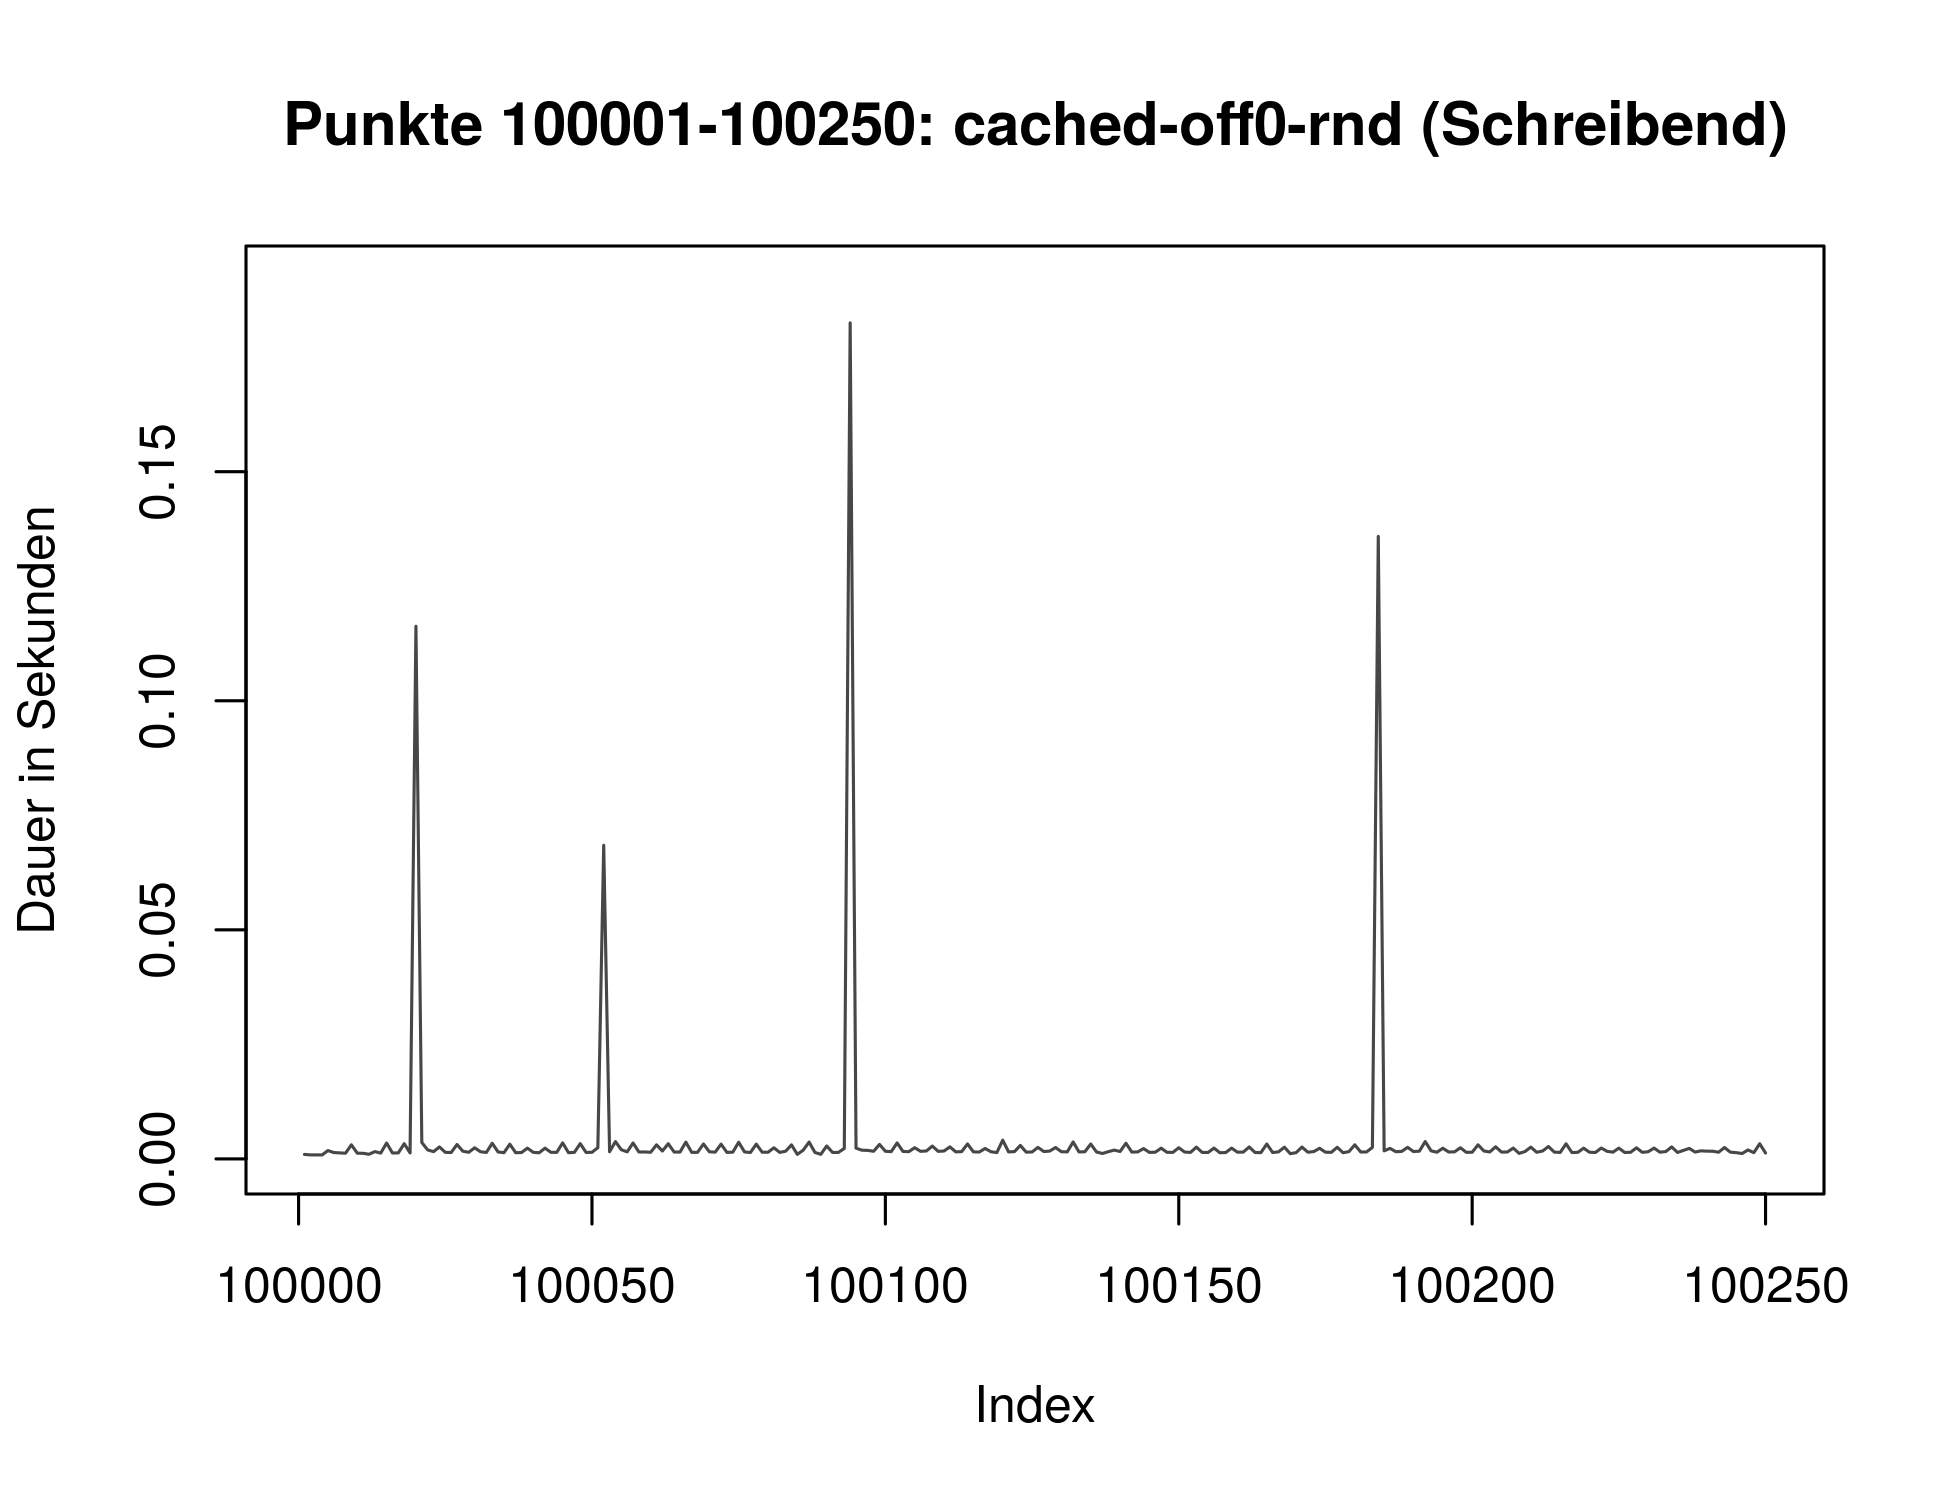
\includegraphics[width=.43\textwidth]{Bilder/Plots/exploration/plot_From100001to100250_write_rnd.png}
	}		
	\caption{Detailbetrachtung der Messungen 100001 bis 100250}
	\label{fig:from100001}
\end{figure} 

\begin{figure}
	\subfloat{
		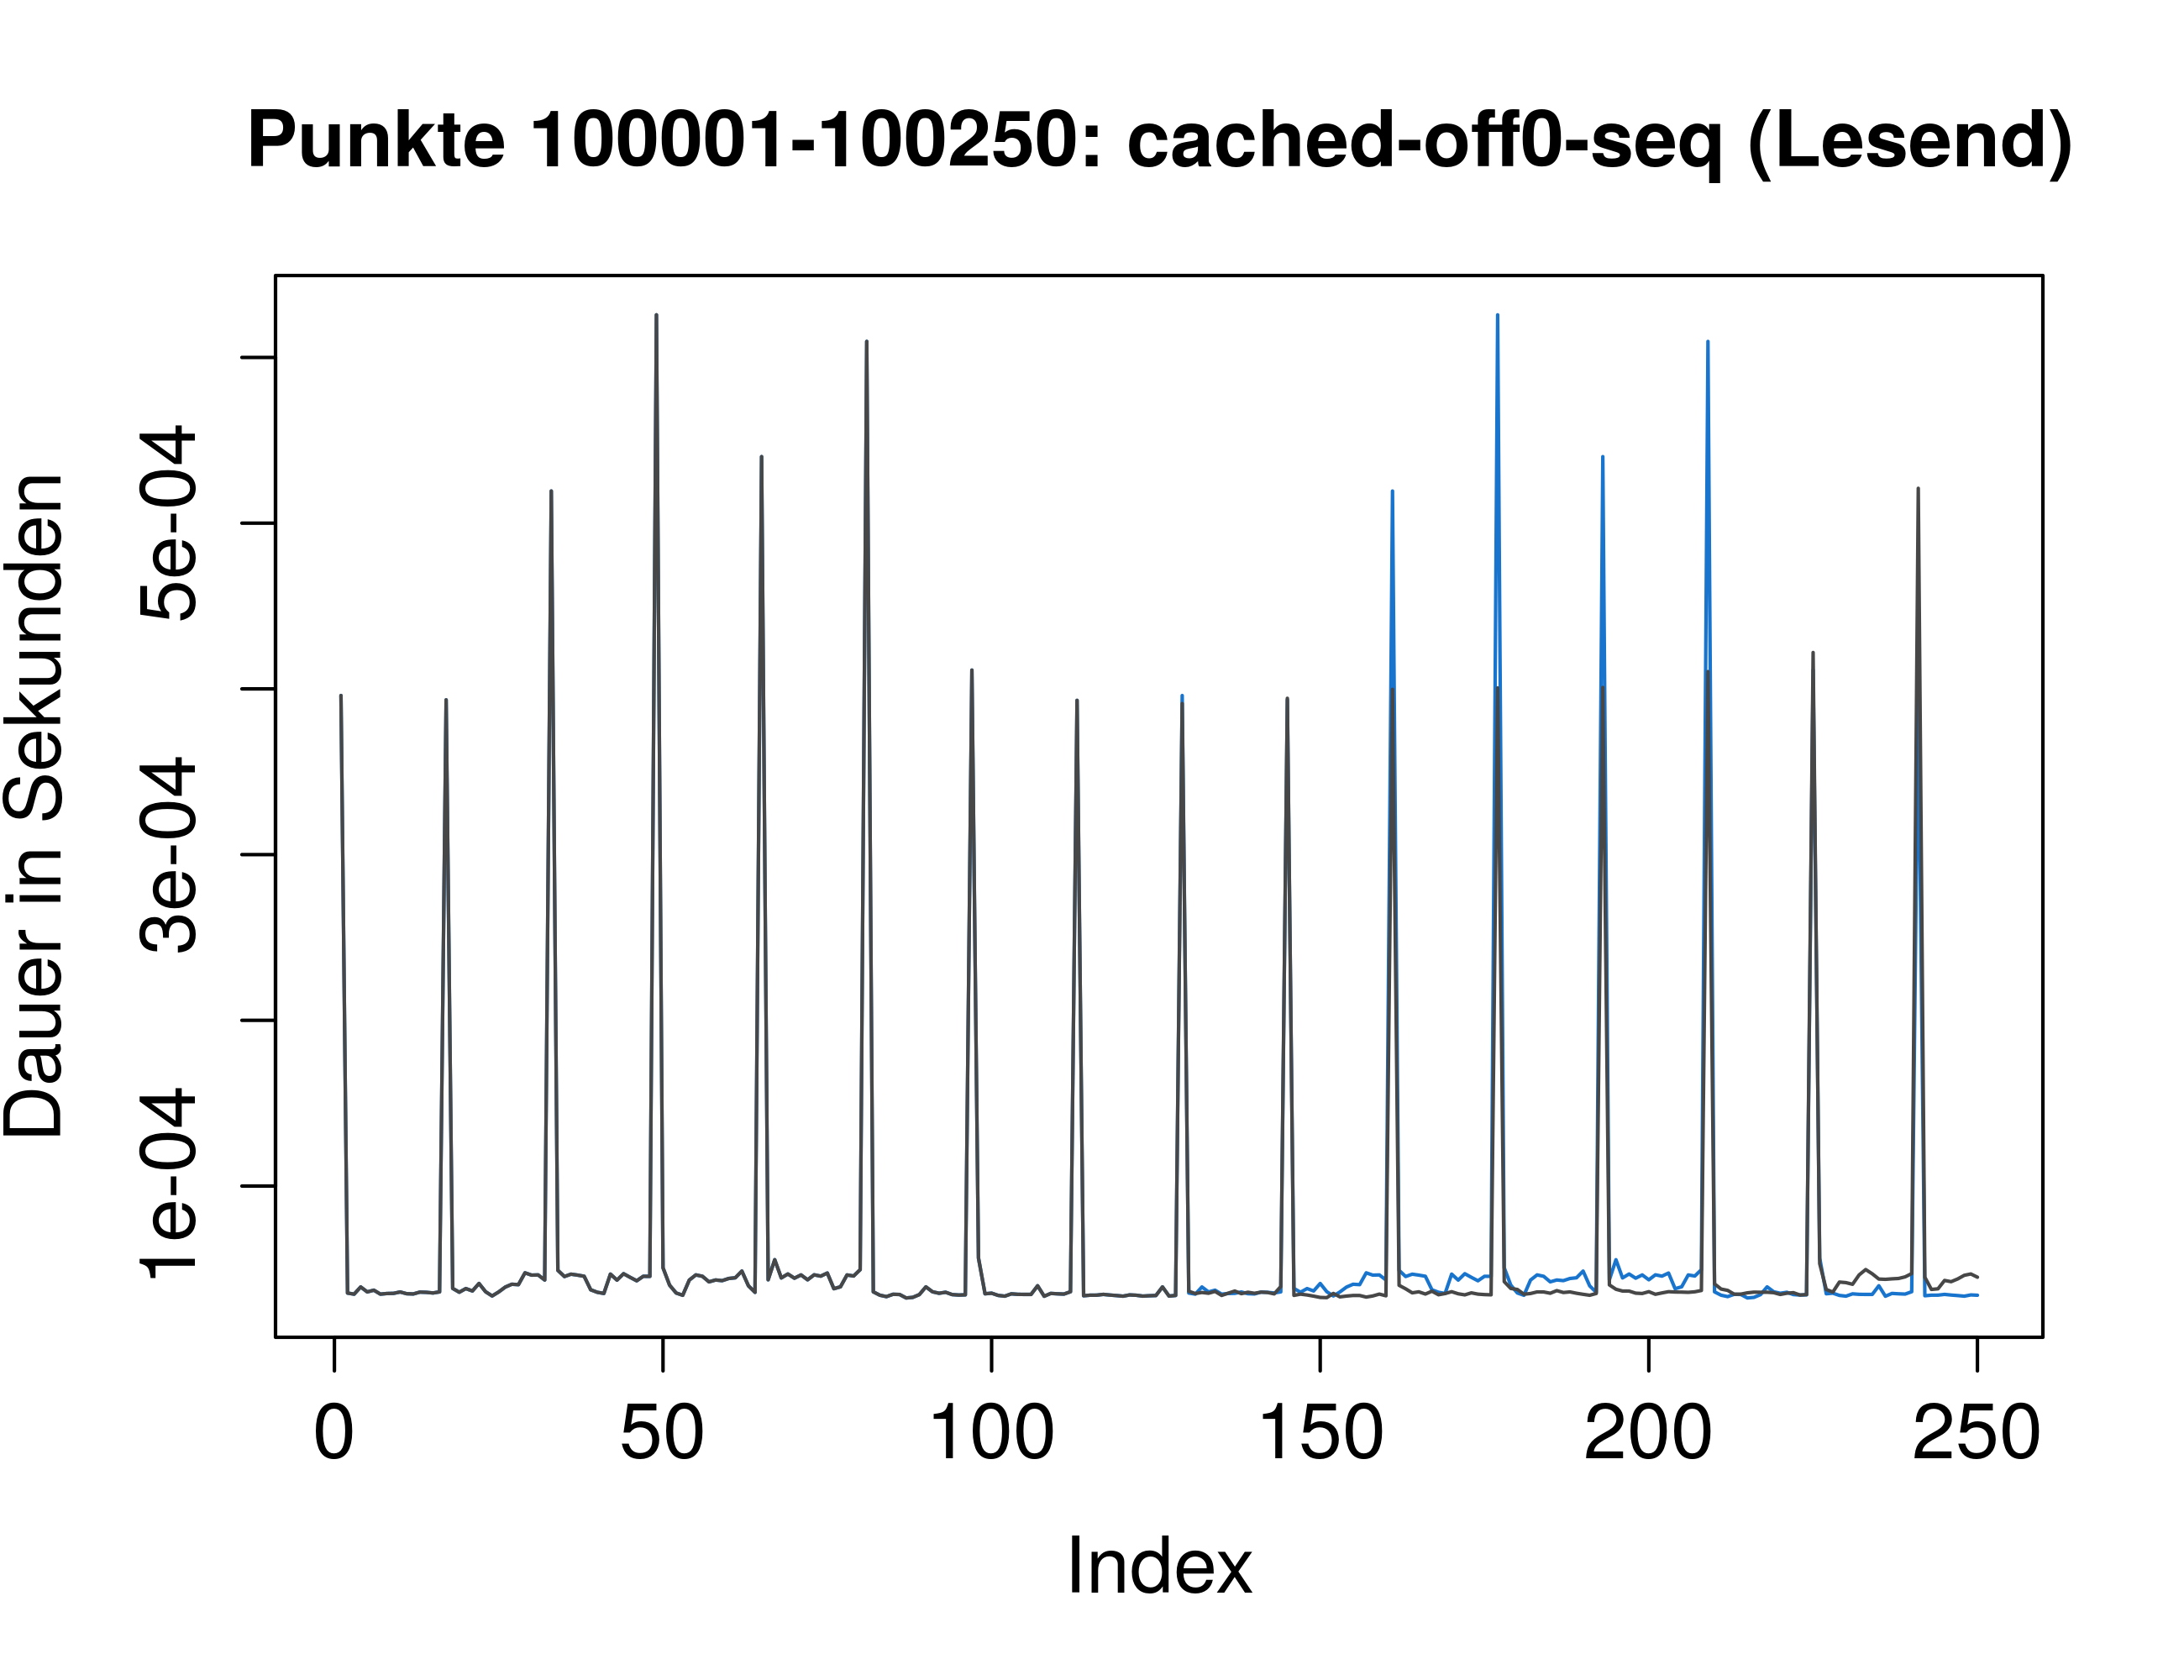
\includegraphics[width=.8\textwidth]{Bilder/Plots/exploration/plot_periodicity100001read_seq.png}
	}	
	\caption{Wiederholung der ersten Werte, als erstes einfaches Modell}
	\label{fig:periodicity100001}
\end{figure} 

\section{Analyse der Fehlerklassen}

Die in \textbf{VERWEIS} eingeführten Fehlerklassen untersuche ich anhand der Ergebnisse, die aus der Clusteranalyse des Fehlers von LinReg G entstanden sind.
In \ref{fig:error_class_clustering_seq} a), sowie \ref{fig:error_class_clustering_rnd} a) ist in Zeitreihe der Fehler aufgezeichnet, den LinReg G auf cached-off0-seq, bzw cached-off0-rnd, mit seinen Vorhersagen gegenüber den tatsächlichen Laufzeiten gemacht hat. In \ref{fig:error_class_clustering_seq} c) und \ref{fig:error_class_clustering_rnd} c) ist das gleiche gezeichnet, allerdings sind die größten und kleinsten Werte weggelassen. Dabei können auf dem Graph zum sequentiellen Datensatz Phasen mit guten und schlechten Vorhersagen erkannt werden. Hier wird ein Verhalten visualisiert, das darauf rückschließen lässt, dass das Modell die Laufzeiten mancher Attribut-Sets besser modelliert hat, als das von anderen. Denn hier wird das selbe Attribut-Set vielfach hintereinander getestet. Der Dateizugriffsort ändert sich bei jedem Zugriff auf dem randomisierten Datensatz und entsprechend ist dieses Verhalten hier nicht so stark ausgeprägt. Auf diesem Datensatz ist dagegen eine unterschiedlich gute Modellierung für Lese- und Schreibzugriffe erkennbar, denn die erste Hälfte der Fehler hat einen flacheren und gleichmäßigeren Verlauf, als die zweite Hälfte, in der die schreibenden Messungen sichtbar sind. \textbf{LÜCKE RECHTs}
In den Graphen jeweils rechts neben den beschriebenen ist durch farbliche Markierung die Zugehörigkeit der Messpunkte zu den unterschiedlichen Klassen erkennbar. Die Unterscheidung in verschiedene Klassen findet in horizontalen Linien statt. Eine Klasse deckt einen bestimmten Bereich der Fehlerwerte ab, die abgedeckten Bereiche lassen sich aus \ref{tab:error_classes_switched} entnehmen. 
Bei der Betrachtung der Graphen mit nach Fehler sortierten Punkten ( \ref{fig:error_class_clustering_seq} e) und f), sowie \ref{fig:error_class_clustering_rnd} e) und f) ) können die Anzahlen der jeweils zugeordneten Punkte zu den Klassen gut quantifiziert werden (die exakten Zahlen sind auch \ref{tab:error_classes_switched} zu entnehmen). In beiden Fällen enthält eine Klasse den Großteil der Punkte (jeweils etwa $3/4$), die Klassen, dessen Bereich leicht abweichen, enthalten noch einen kleinen Anteil der Messdaten. Die Ausreißer in beide Richtungen machen quantitativ fast nichts aus, werden allerdings durch mehrere Klassen abgedeckt. So werden die obersten \textbf{WERT} \% der Daten auf cached-off0-rnd in 6 Klassen aufgeteilt.\\
Das Modell scheint generell schon recht gut zu sein, da die Fehler sich für die Klassen mit dem kleinsten durchschnittlichen Fehler sammeln. Es gibt allerdings einige Datenpunkte, die das Modell sehr schlecht vorhersagen konnte. Die Annahme ist nun, dass die voneinander stark abweichenden Datenpunkte grundsätzlich unterschiedlich vom System verarbeitet wurden. Sodass die Fehlerklassen die unterschiedlichen E/A-Wege im System repräsentieren. 
Ein Modell, dass eine Modellierung mit dem zusätzlichen Wissen dieser Klassenzuordnungen vornimmt, sollte die Ausreißer, die LinReg G schlecht bestimmt hat, wesentlich besser vorhersagen können. Für die Vorhersage der vielen Datenpunkte, die sich in der jeweils größten Klasse befinden, hat ein Modell mit Fehlerklasseninformationen jedoch keine weiteren Vorteile. 

\begin{figure}
	\centering
	\subfloat[Fehler des Modells \glqq LinReg G\grqq{} auf cached-off0-seq, in Zeitreihe]{
		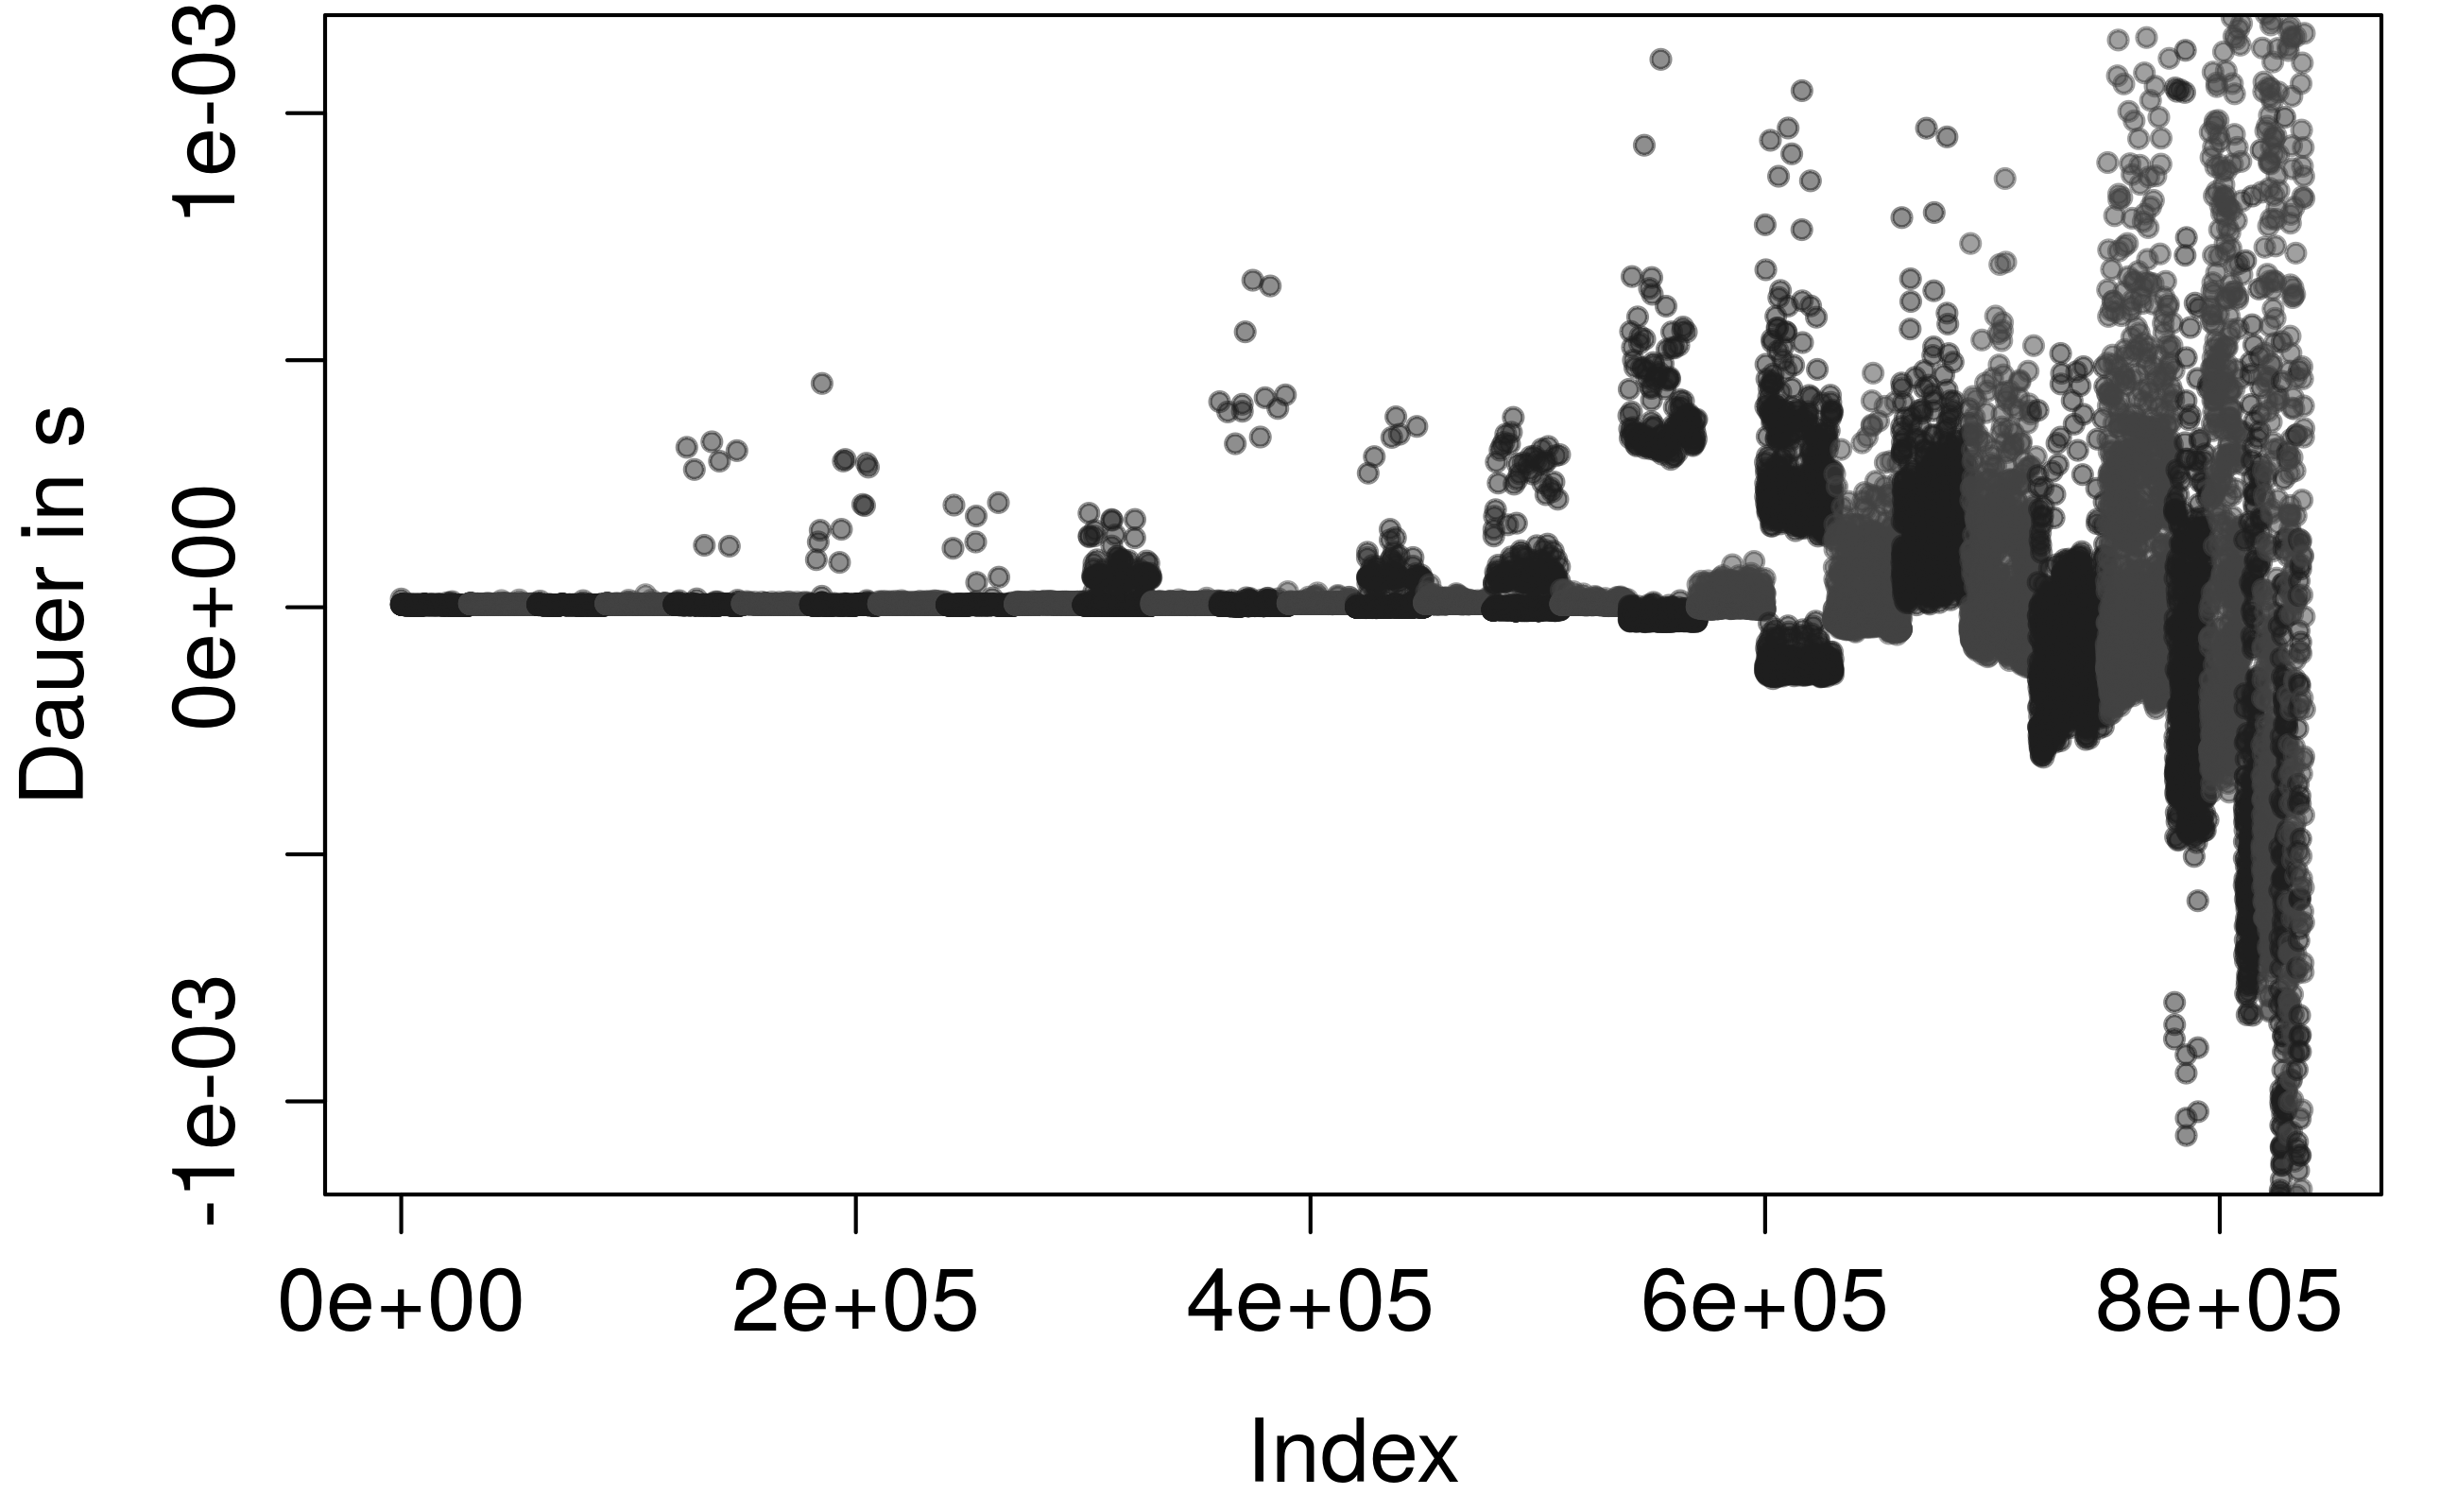
\includegraphics[width=.43\textwidth]{Bilder/Plots/error_class/exploration/linreg_error_seq_all.png}
	}
	\subfloat[Farblich markierte Fehlerklassen]{
		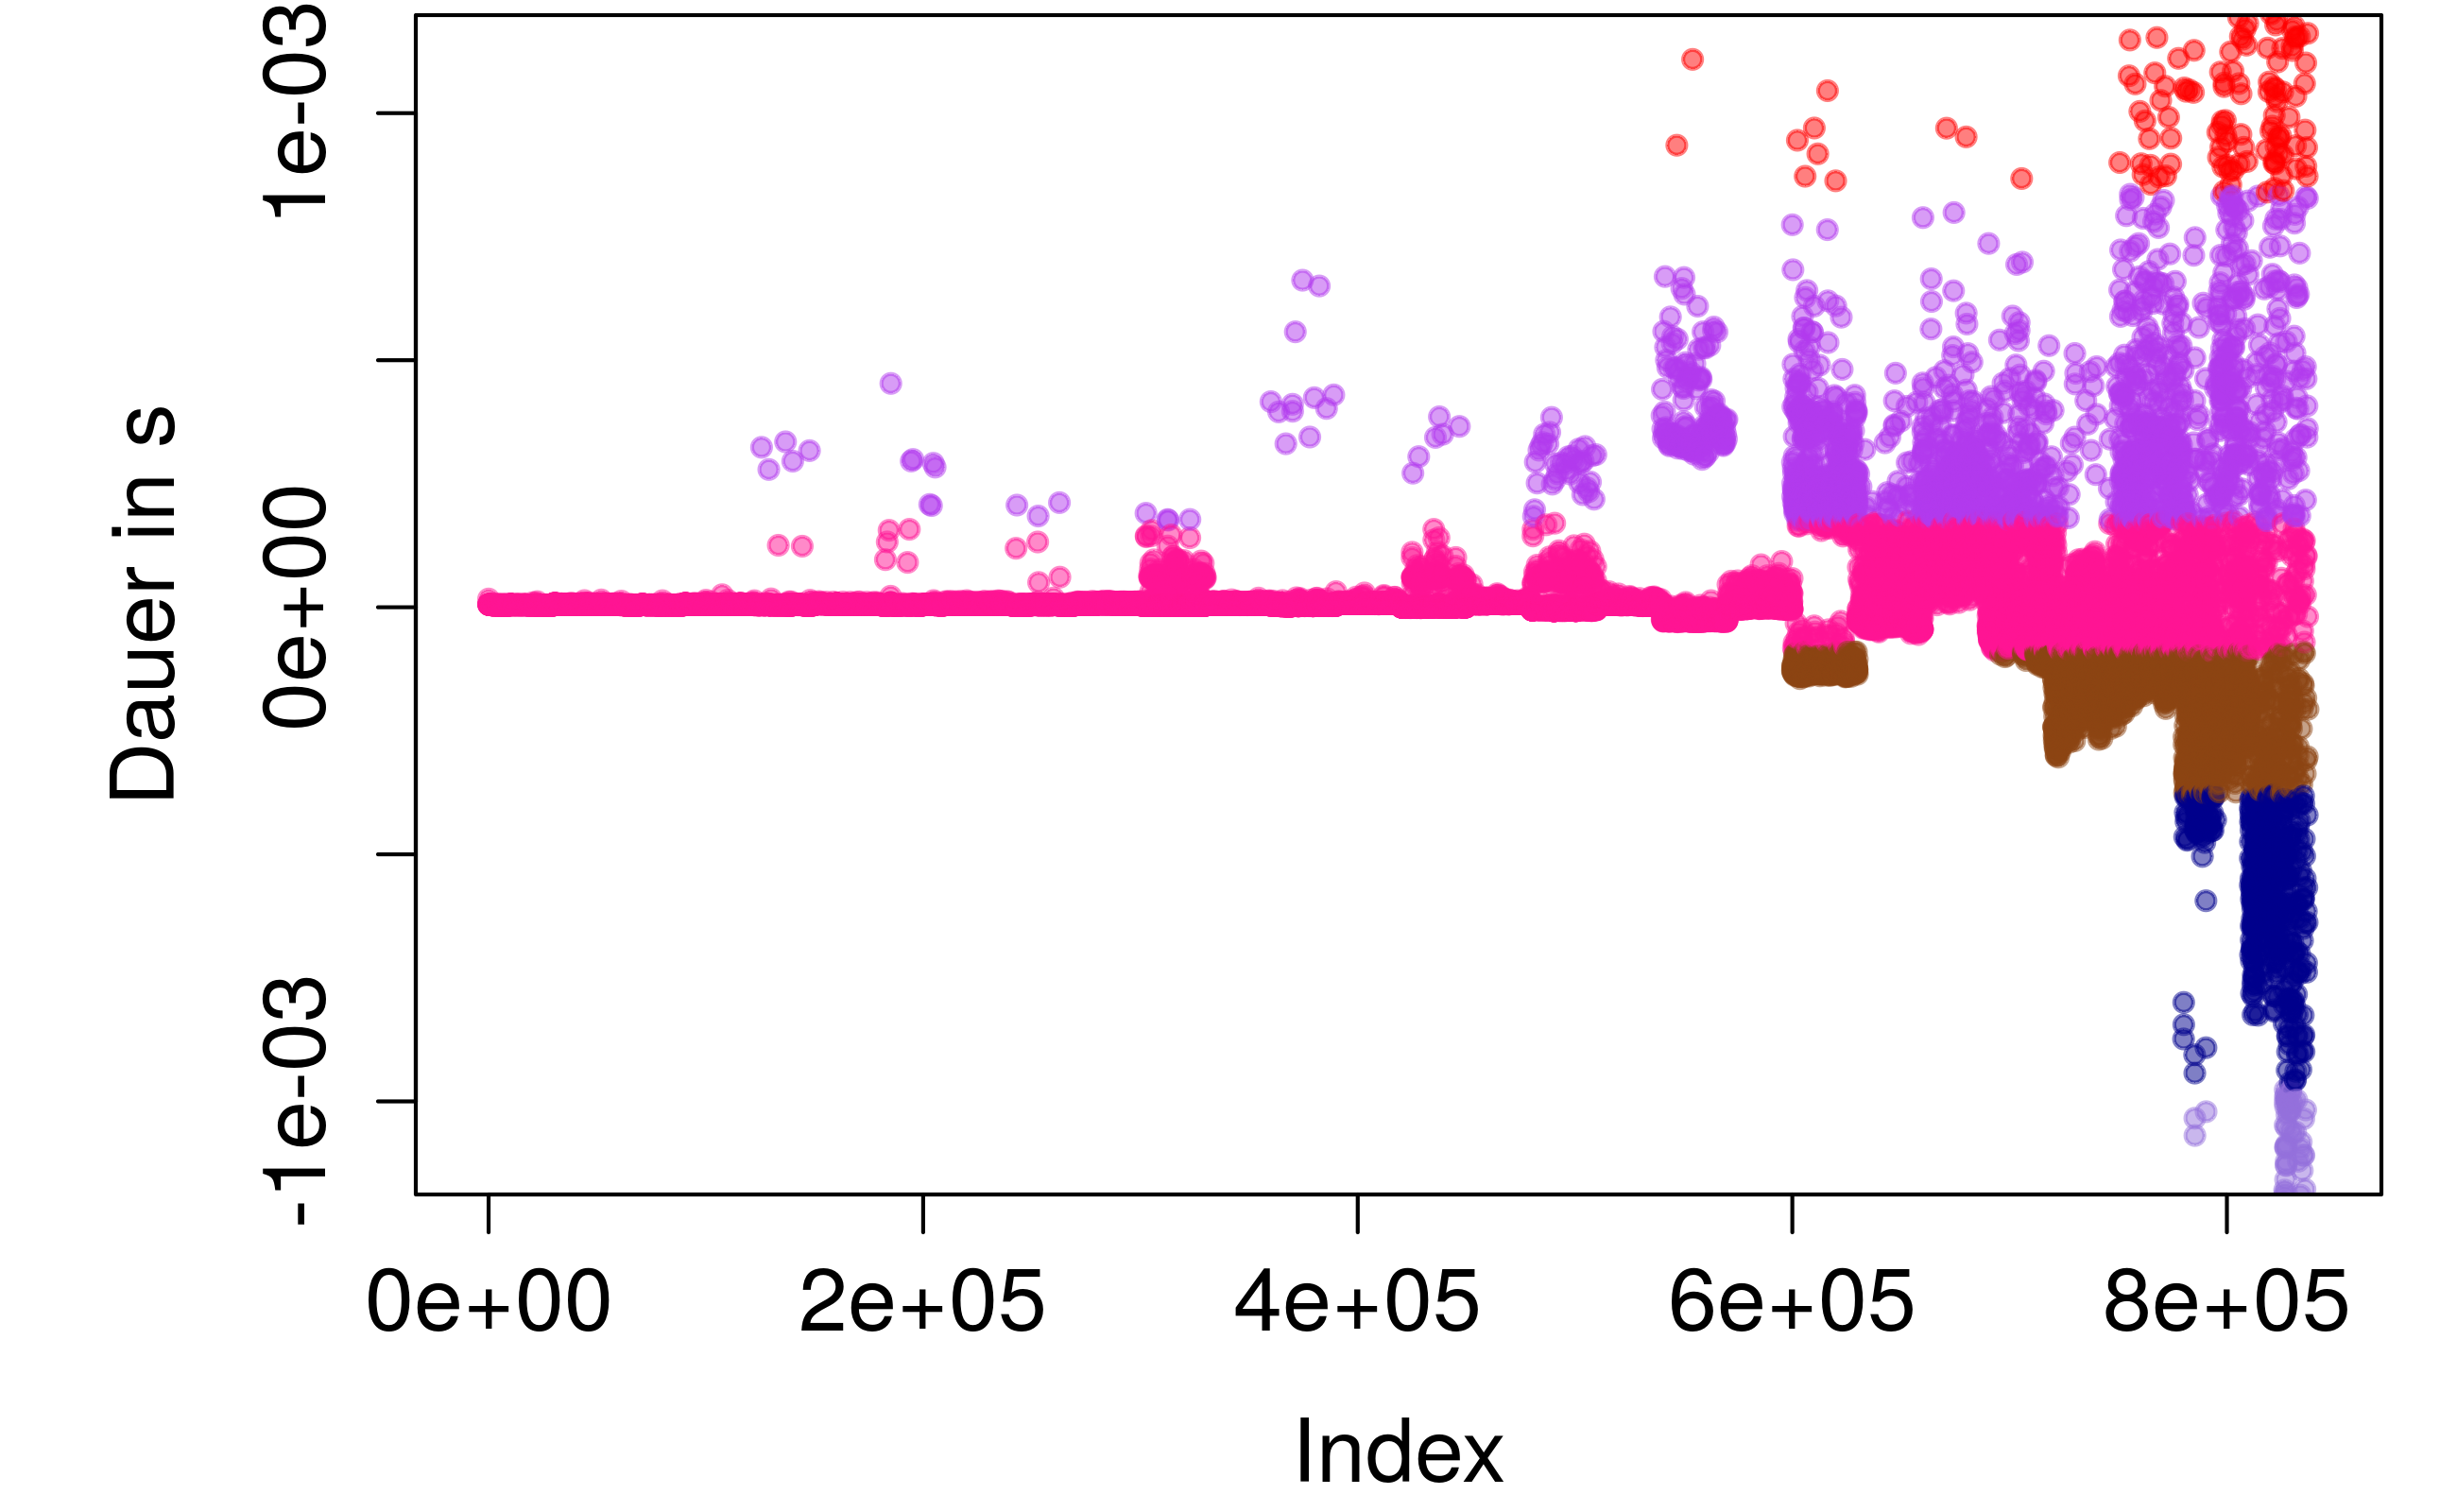
\includegraphics[width=.43\textwidth]{Bilder/Plots/error_class/exploration/linreg_error_clustering_seq_all.png}
	}\\
	\subfloat[Fehler des Modells \glqq LinReg G\grqq{} auf cached-off0-seq, in Zeitreihe, ohne die äußersten 1\%]{
		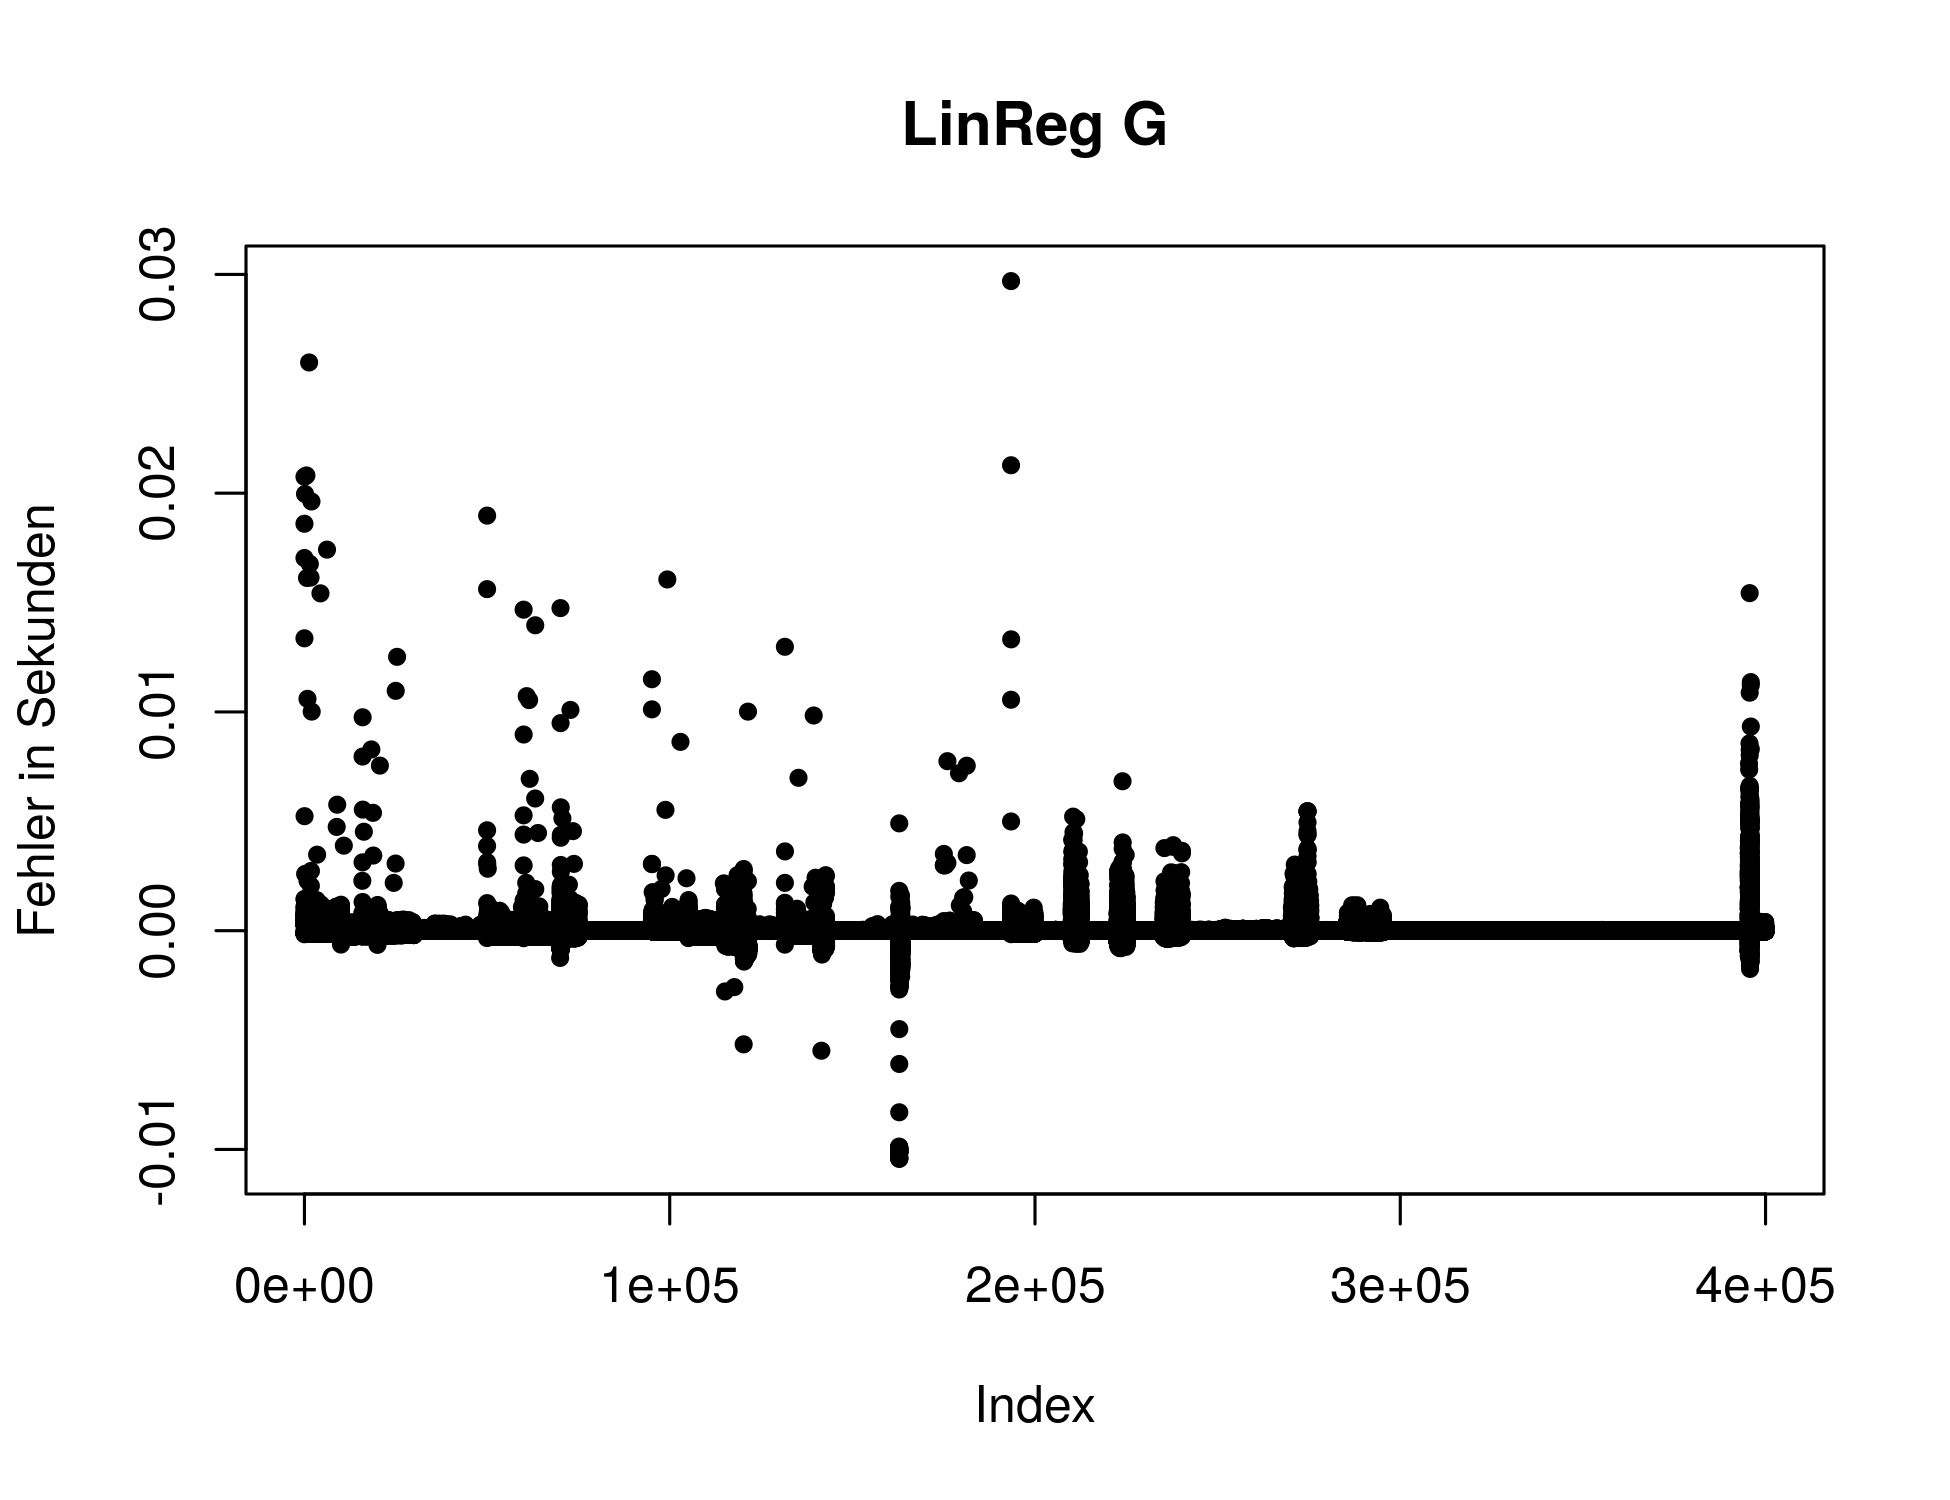
\includegraphics[width=.43\textwidth]{Bilder/Plots/error_class/exploration/linreg_error_seq.png}
	}
	\subfloat[Farblich markierte Fehlerklassen, ohne die äußersten 1\%]{
		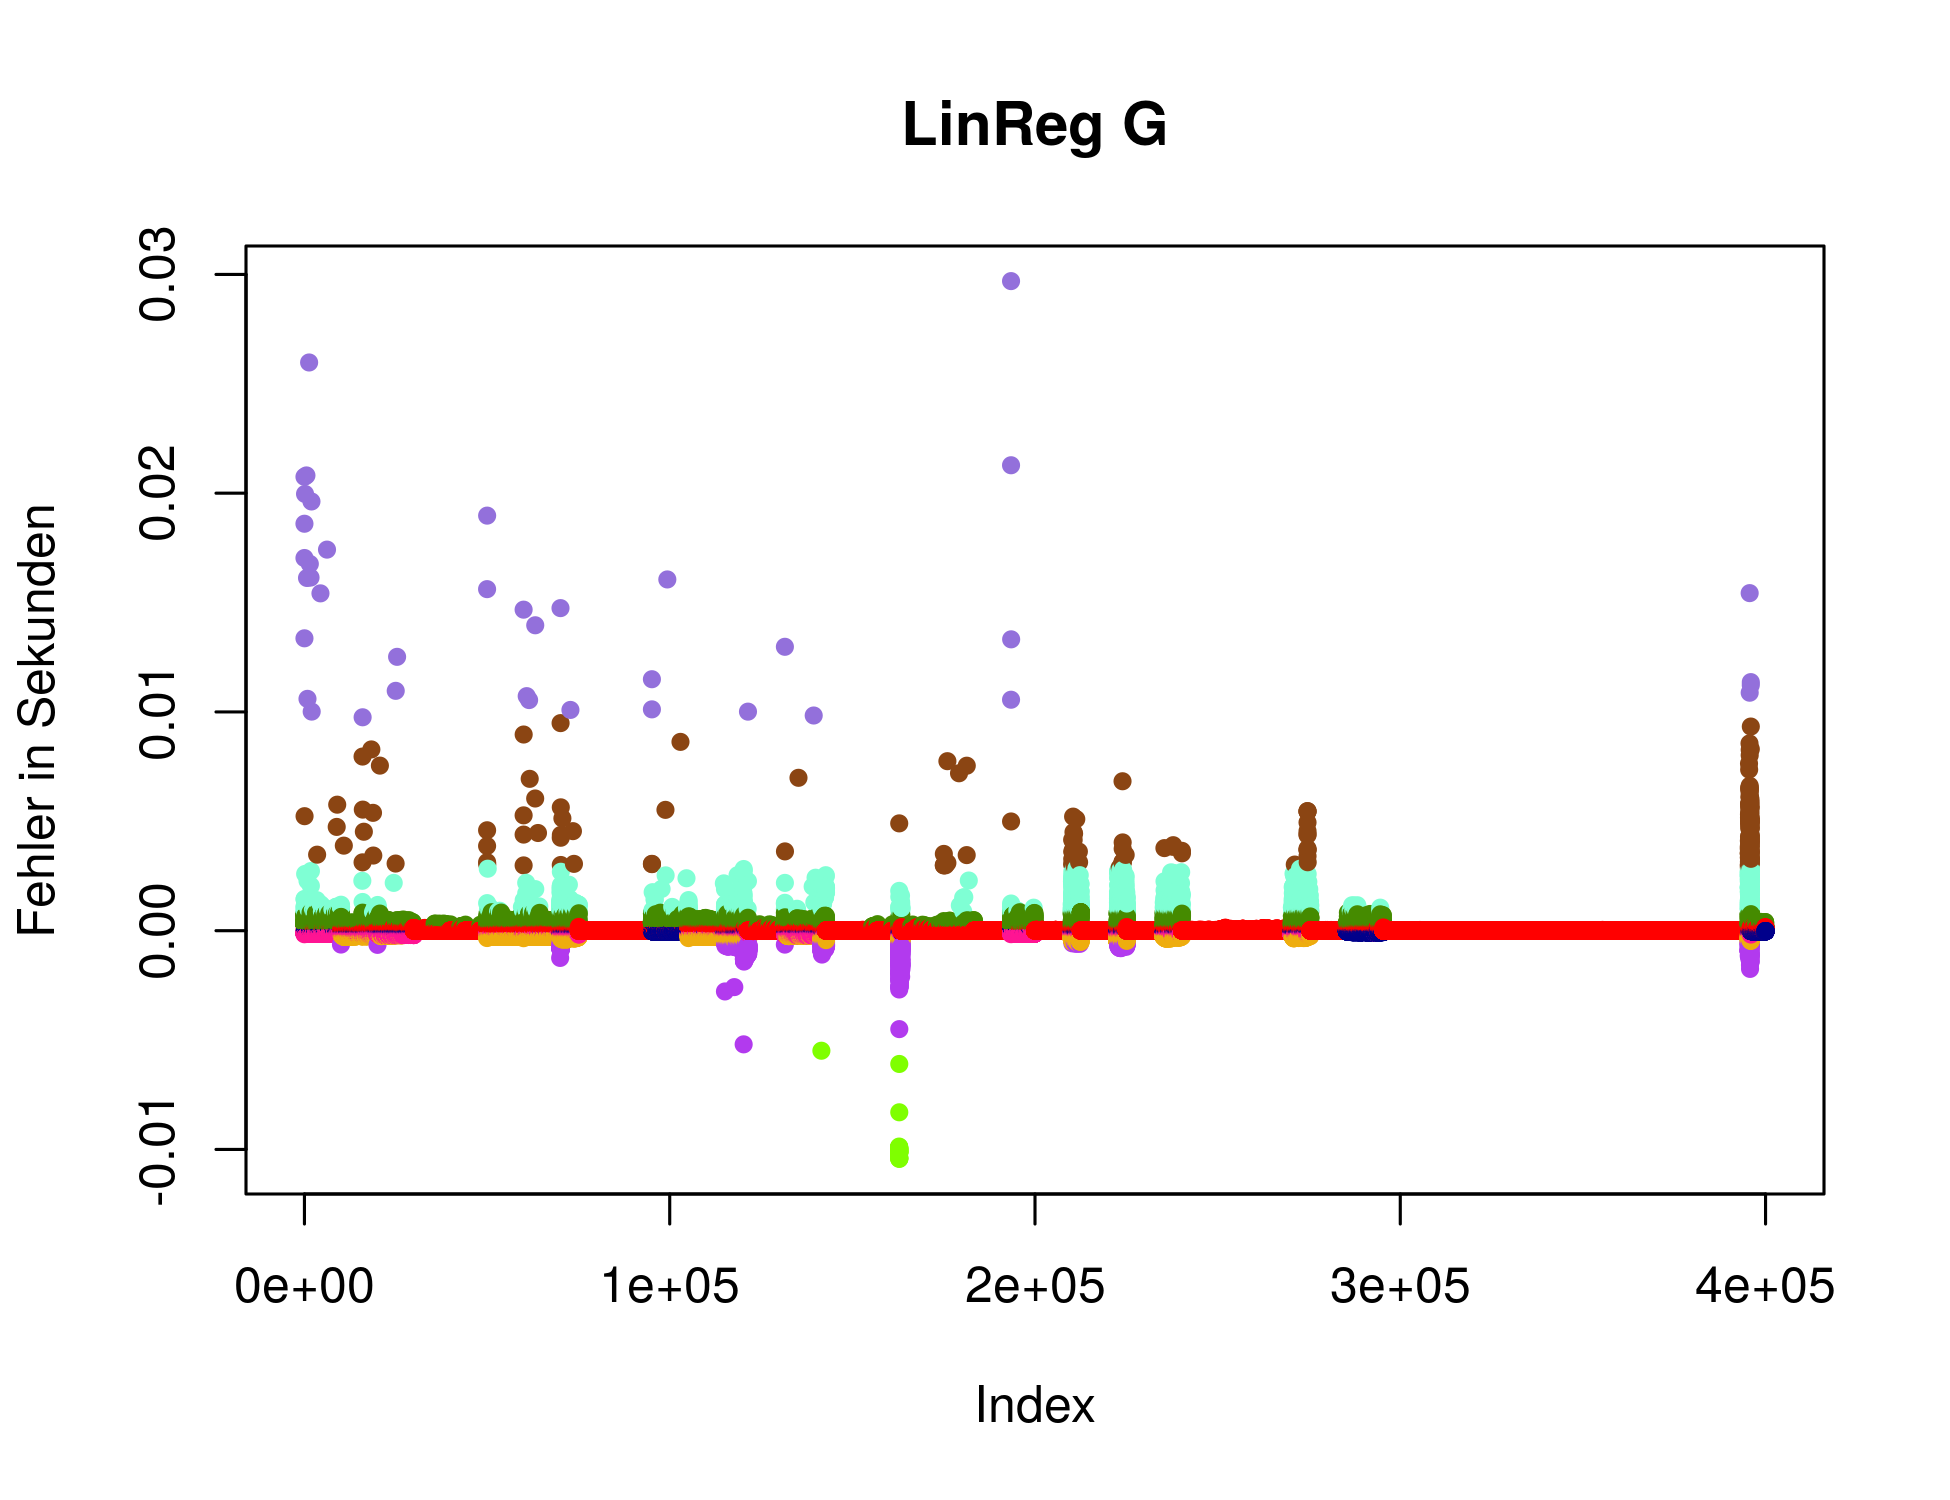
\includegraphics[width=.43\textwidth]{Bilder/Plots/error_class/exploration/linreg_error_clustering_seq.png}
	}\\
	\subfloat[Fehler des Modells \glqq LinReg G\grqq{} auf cached-off0-seq, sortiert]{
		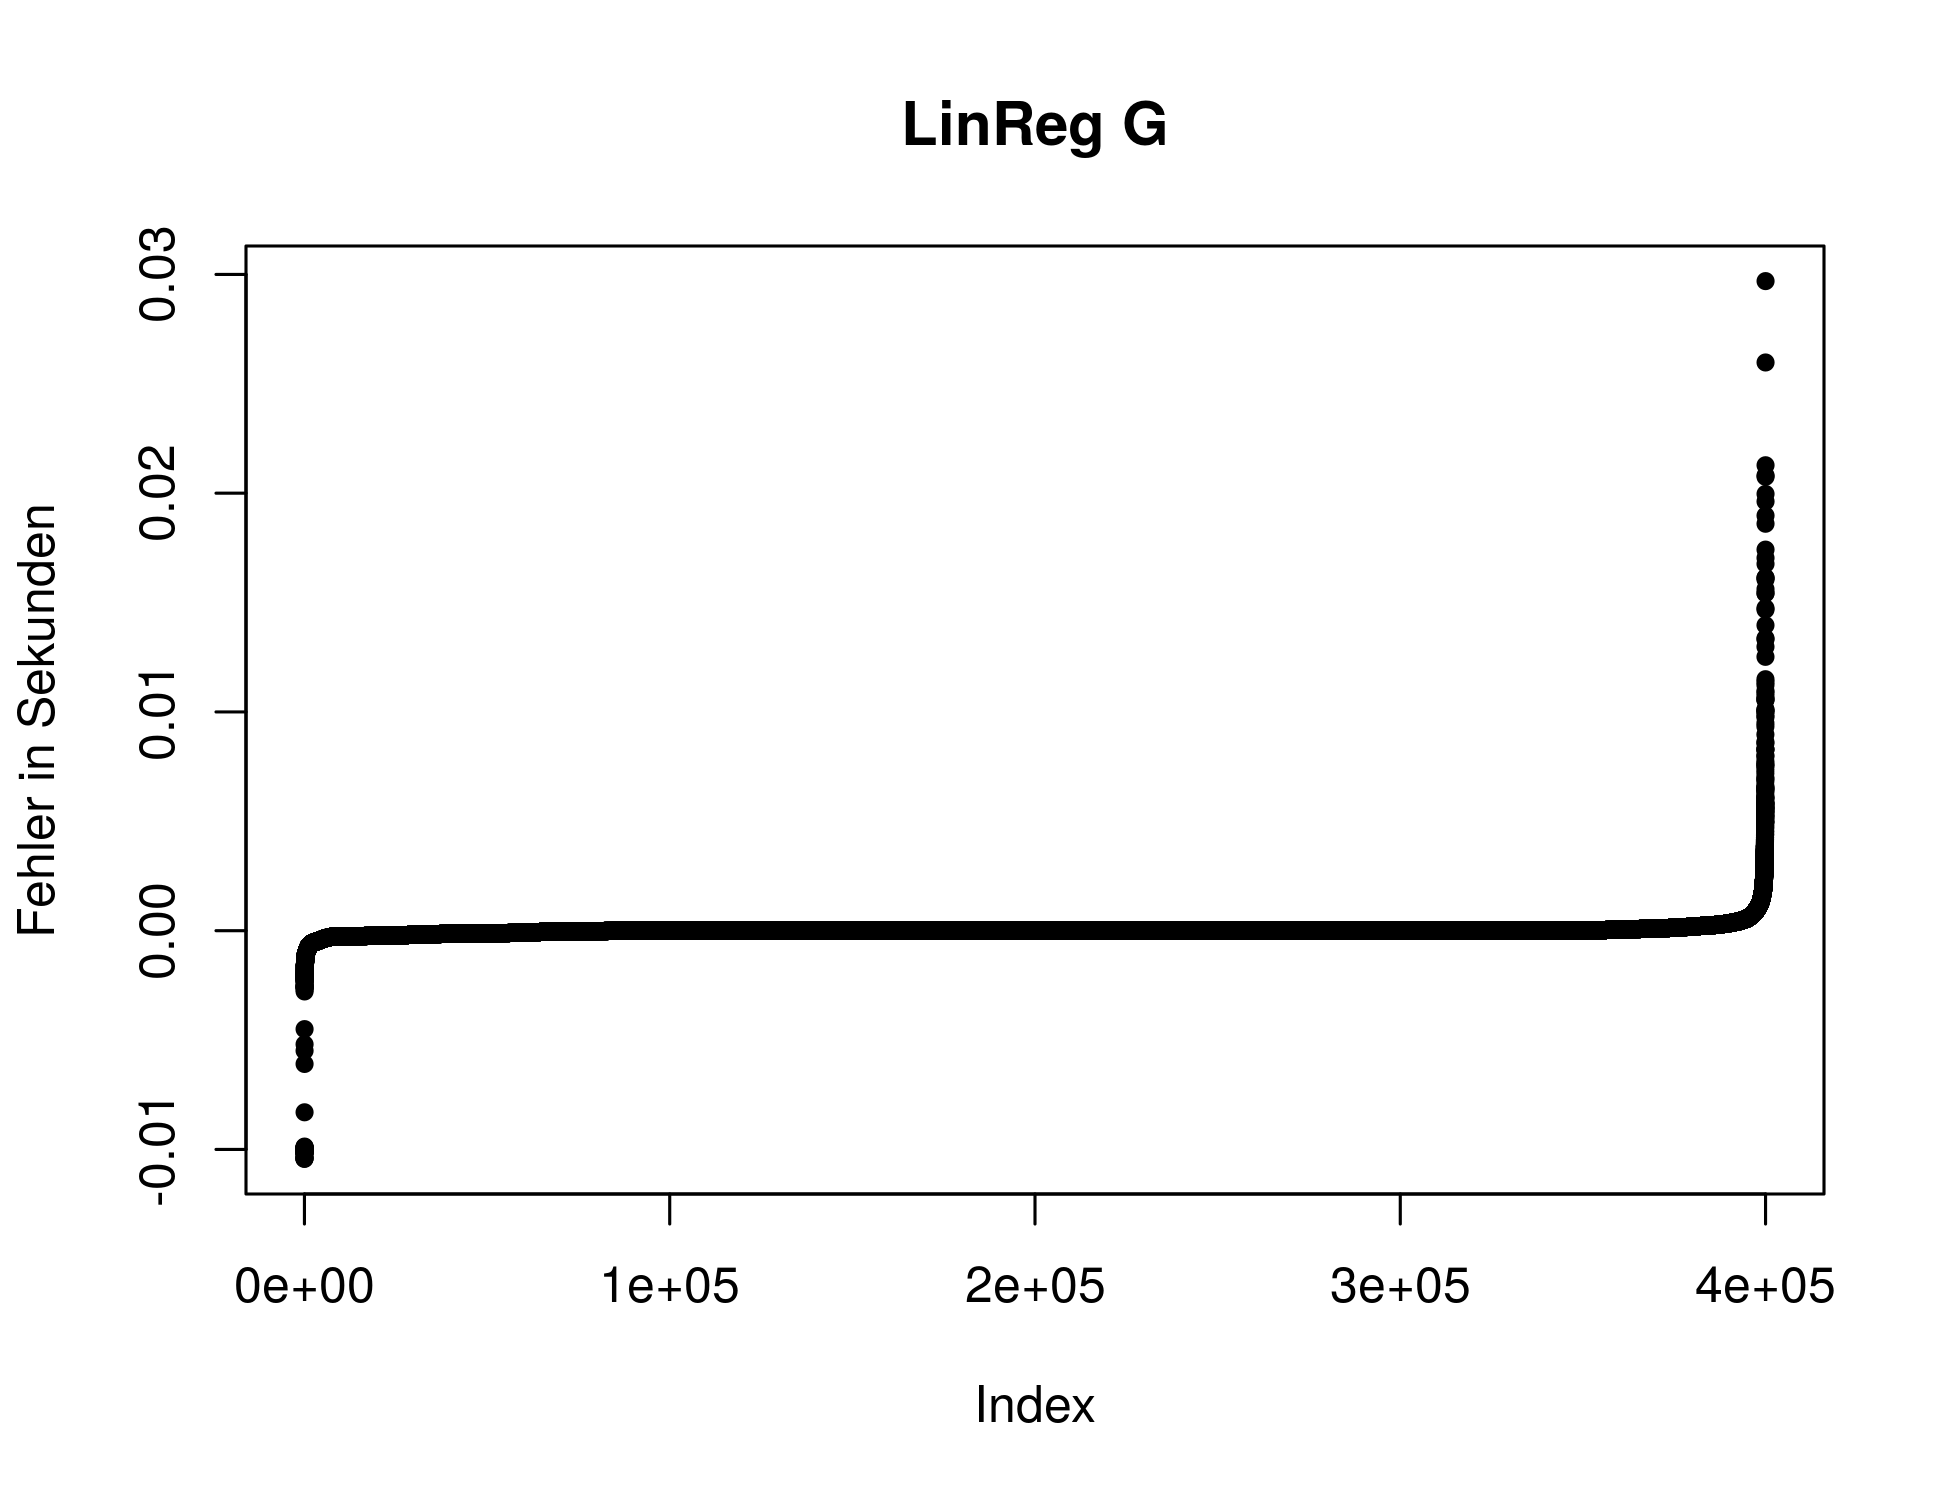
\includegraphics[width=.43\textwidth]{Bilder/Plots/error_class/exploration/linreg_error_sorted_seq.png}
	} 	
	\subfloat[Farblich markierte Fehlerklassen]{
		\includegraphics[width=.43\textwidth]{Bilder/Plots/error_class/exploration/linreg_error_sorted_clustering_seq.png}
	}\\	
	\caption{Verwendung des K-Means Algorithmus zur Bestimmung der Fehlerklassen auf cached-off0-rnd mit der Vorhersage von \glqq LinReg G\grqq}
	\label{fig:error_class_clustering_seq}
\end{figure} 

\begin{figure}
	\centering
	\subfloat[Fehler des Modells \glqq LinReg G\grqq{} auf cached-off0-rnd, in Zeitreihe]{
		\includegraphics[width=.43\textwidth]{Bilder/Plots/error_class/exploration/linreg_error_rnd_all.png}
	}
	\subfloat[Farblich markierte Fehlerklassen]{
		\includegraphics[width=.43\textwidth]{Bilder/Plots/error_class/exploration/linreg_error_clustering_rnd_all.png}
	}\\
	\subfloat[Fehler des Modells \glqq LinReg G\grqq{} auf cached-off0-rnd, in Zeitreihe, ohne die äußersten 1\%]{
		\includegraphics[width=.43\textwidth]{Bilder/Plots/error_class/exploration/linreg_error_rnd.png}
	} 	
	\subfloat[Farblich markierte Fehlerklassen, ohne die äußersten 1\%]{
		\includegraphics[width=.43\textwidth]{Bilder/Plots/error_class/exploration/linreg_error_clustering_rnd.png}
	}\\
	\subfloat[Fehler des Modells \glqq LinReg G\grqq{} auf cached-off0-rnd, sortiert]{
		\includegraphics[width=.43\textwidth]{Bilder/Plots/error_class/exploration/linreg_error_sorted_rnd.png}
	} 	
	\subfloat[Farblich markierte Fehlerklassen]{
		\includegraphics[width=.43\textwidth]{Bilder/Plots/error_class/exploration/linreg_error_sorted_clustering_rnd.png}
	}\\
	\caption{Verwendung des K-Means Algorithmus zur Bestimmung der Fehlerklassen auf cached-off0-rnd mit der Vorhersage von \glqq LinReg G\grqq}
	\label{fig:error_class_clustering_rnd}
\end{figure} 

Anhand einer weiteren Betrachtung der Fehlerklassen sollen die Unterschiede zwischen den Klassen auf den beiden Datensätzen analysiert werden.
In Abbildung \ref{fig:error_classes_switched} sind die Punkte den Klassen aus dem jeweils anderen Datensatz zugeordnet worden. Die Neuzuordnung wurde ebenso durchgeführt, wie es der K-Means Algorithmus bei der Erstzuordnung gemacht hat. Für alle Klassen wurde der mittlere Fehlerwert nach Zuordnung der Punkte auf dem ursprünglichen Datensatz berechnet und dann wurde jeder Datenpunkt im anderen Datensatz der Klasse mit dem Mittelwert zugeordnet, der am nächsten an seinem eigenen Fehlerwert liegt.\\ 
Für cached-off0-seq ist deutlich zu sehen (\ref{fig:error_classes_switched} c) ), dass 99\% der Punkte der selben Fehlerklasse zugeordnet worden. Dagegen wird bei cached-off-rnd in dem Bereich mit kleinerem Fehler nun stärker als zuvor (\ref{fig:error_class_clustering_rnd} d) ) differenziert, während alle größeren Fehler die selbe Klasse haben.

\begin{figure}
	\centering
	\subfloat[Klassen aus cached-off0-rnd auf cached-off0-seq]{
		\includegraphics[width=.43\textwidth]{Bilder/Plots/error_class/exploration/rnd_linreg_classes_on_seq_all.png}
	}
	\subfloat[Klassen aus cached-off0-seq auf cached-off0-rnd]{
		\includegraphics[width=.43\textwidth]{Bilder/Plots/error_class/exploration/seq_linreg_classes_on_rnd_all.png}
	}\\
	\subfloat[Klassen aus cached-off0-rnd auf cached-off0-seq, ohne die äußersten 1\%]{
		\includegraphics[width=.43\textwidth]{Bilder/Plots/error_class/exploration/rnd_linreg_classes_on_seq.png}
	}
	\subfloat[Klassen aus cached-off0-seq auf cached-off0-rnd, ohne die äußersten 1\%]{
		\includegraphics[width=.43\textwidth]{Bilder/Plots/error_class/exploration/seq_linreg_classes_on_rnd.png}
	}
	\caption{Farblich markierte Fehlerklassen, unter Verwendung der Fehlerklassen, die aus aus dem jeweils anderen Datensatz stammen}
	\label{fig:error_classes_switched}
\end{figure} 

In \ref{tab:error_classes_switched} wurden die Fehlerklassen nun nach mittleren Durchsatz sortiert. (\textbf{WARUM?}) \textbf{BESCHREIBUNG DER TABLLE}
In der Tabelle ist ablesbar, was ich zuvor bereits anhand des Graphen gedeutet habe, für cached-off0-seq befinden sich mit vertauschten Fehlerklassen 399709 von 400000 Punkten in der selben Klasse. Dies ist die Klasse, die den geringsten Durchsatz hat und in der LinReg G zuvor auf dem randomisierten Datensatz den größten Fehler gemacht hat.
Die Fehlerklassen von cached-off0-seq sind dagegen sogar recht gut zur Differenzierung der Datenpunkte auf cached-off0-rnd nutzbar, wie in Tabelle \ref{tab:error_classes_switched} b) an den Werten für \glqq Anzahl auf rnd \grqq{} zu entnehmen ist. Dies ist dem Umstand geschuldet, dass die Fehlerklassen von cached-off0-seq in dem Bereich mit kleinem Fehler stark differenziert und die meisten Punkte sich auch auf cached-off0-rnd dort befinden.
Für eine bessere Vorhersage der Messdaten würden sich diese Klassen auf beiden Datensätzen nicht eignen. Auf cached-off0-seq, da sich praktisch alle Punkte in der selben Klasse befinden und auf cached-off0-rnd, weil in den entscheidenden schlechteren Vorhersagen von LinReg G keine Unterscheidung stattfindet.

\begin{table}
	\scriptsize
	\subfloat[Fehlerklassen von cached-off0-seq]{
		\begin{tabular}{|r|r|r|r|r|r|r|}\hline%
			Klasse & mittlerer Durchsatz (B/s) & Min (s) & Durchschnitt (s) & Max (s) & Zugeordnet auf seq & Zugeordnet auf rnd \\\hline\hline
			\csvreader[late after line=\\\hline]%
			{CSV/error_class/seq_linreg_classes_on_rnd.csv}{tp=\tp,idx = \idx,rndcount=\rndcount,minerror=\minerror, meanerror = \meanerror, maxerror = \maxerror, seqcount = \seqcount}%
			{\idx & \tp & \minerror & \meanerror & \maxerror & \seqcount & \rndcount}%
		\end{tabular}
	}\\
	\subfloat[Fehlerklassen von cached-off0-rnd]{
		\begin{tabular}{|r|r|r|r|r|r|r|}\hline%
			Klasse & mittlerer Durchsatz (B/s) & Min (s) & Durchschnitt (s) & Max (s) & Zugeordnet auf rnd & Zugeordnet auf seq \\\hline\hline
			\csvreader[late after line=\\\hline]%
			{CSV/error_class/rnd_linreg_classes_on_seq.csv}{tp=\tp,idx = \idx, rndcount=\rndcount,minerror=\minerror, meanerror = \meanerror, maxerror = \maxerror, seqcount = \seqcount}%
			{\idx & \tp & \minerror & \meanerror & \maxerror & \rndcount & \seqcount}%
		\end{tabular}
	}
	
	\caption{Fehlerklassen sortiert von kleinem zu großem Zentrum des Clusters (Durchschnittlicher Fehler). Einmal die Anzahl Punkte, die den Klassen auf dem Datensatz zugeordnet wurden, von dem sie auch stammen. Zudem die Anzahl Punkte, die den Klassen auf dem anderen Datensatz zugeordnet werden würden.}
	\label{tab:error_classes_switched}
\end{table}

\section{Leistungsvorhersage}
Zu jedem Modell schreiben, welche Attribute und Parameter sich als geeignet herausgestellt haben. Ergebnisse anhand von Graphen veranschaulichen.\\
Ergebnisse für verschiedene Fälle vergleichen, seq,rnd\\
Ergebnisse von bagging

\subsection{Analyse der trivialen Modelle}

Die Ergebnisse der in \textbf{ABSCHNITT} beschriebenen trivialen Modelle sind in \ref{tab:triv} zu sehen. Eine positive Beobachtung in den Ergebnissen auf cached-off0-seq ist zunächst, dass alle Metriken einen ähnlichen Trend der  Modelle aufzeichnen. Das gilt im Wesentlichen auch für cached-off0-rnd, jedoch hat das Modell "Median agg" einen sehr hohen maximalen Fehler. Dies führt entsprechend zu einem vergleichsweise hohen RMQA-Wert, obwohl der relative arithmetische Fehler noch recht gering ist. \\
Wie erwartet (\textbf{ABSCHNITT}) sind die Vorhersagen auf dem randomisierten Datensatz schwieriger zu machen, sodass die Fehlerwerte höher sind. Dies gilt insbesondere für die Modelle, die auf linearer Regression basieren, hier sind die Werte $30-140$ mal höher. Eine Ausnahme ist "Median agg LinReg-Fehlerklasse", das Modell kann eine weiterhin sehr gute mittlere Vorhersage treffen, nur die Ausreißer nach oben scheinen zugenommen zu haben, sodass RMax und RMQA höher als bei sequentiellen Datensatz sind.\\
Allgemein sind die Ergebnisse bereits überraschend gut. Ein durchschnittlicher Fehler von $5\%$ auf cached-off0-seq bzw. $7-12\%$ auf cached-off0-rnd durch die Modelle, die Fehlerklassen ausnutzen, deutet daraufhin, dass die Vorgänge im E/A-System im Wesentlichen korrekt repräsentiert werden. Ob über eine größere Messreihe ein geringerer durchschnittlicher Fehler als $5\%$ überhaupt erreicht werden kann, ist fraglich, da das Messrauschen durch unvorhersehbare Ereignisse sowohl auf System-, als auch Bauteilebene, in diesen Bereichen eine zu große Bedeutung zukommt.\\
Die Modelle mit linearer Regression führen auf cached-off0-seq auch bereits zu zufriedenstellenden Ergebnissen, während sie auf cached-off0-rnd kaum sinnvolle Vorhersagen machen zu scheinen. Die Modelle lassen sich für die Datensätze jeweils in drei Gruppen (gut, mittel, schlecht) unterteilen. Auf beiden Datensätzen führen die beiden Modelle mit Fehlerklasse zu einer guten Vorhersage. "Median agg" hat jeweils eine mittel gute Leistung, während "Durchschnitt" jeweils schlecht ist. Interssant ist, dass Modelle mit linearer Regression auf dem sequentiellen Datensatz eine zufriedenstellende mittlel gute Vorhersage macht, während die Vorhersage auf dem randomisierten Messungen kaum besser als des Durschnitts-Modell ist. \\ 
Das Modell, das immer die Durchschnittsdauer vorhersagt ist als absolute untere Grenze für angewendete Modelle zu verstehen, da hier praktisch keine Expertise über die Daten eingeht. 
Tatsächlich erreicht dieses Modell die schlechtesten Ergebnisse in beiden Testfällen. Die Ansätze der rechenintensiven halten diesem Anspruch also stand und sind somit gerechtfertigt. \\
Aufgrund des geringen Nutzen der Attribute Abstand und OpTyp für die lineare Regression wird im Folgenden nur das Modell über die Zugriffsgröße betrachtet.\\

\begin{table}
	\scriptsize
	\subfloat[cached-off0-seq]{
		\begin{tabular}{|r|r|r|r|r|r|r|}\hline%
			Modell & MAF (s)  & RMAF (\%) & RMQA (\%) & RQ3 (\%) & RMax (\%) & Typ \\\hline\hline
			\csvreader[late after line=\\\hline]%
			{CSV/baselines/latex_baseline_seq_results.csv}{Modell=\Model,MAF=\MAF,RMAF=\RMAF, RMQA = \RMQA, Q3 = \Q3, Max = \Max, Typ = \Typ}%
			{\Model & \MAF & \RMAF & \RMQA & \Q3 & \Max & \Typ}%
		\end{tabular}
	} \\
	\subfloat[cached-off0-rnd]{
		\begin{tabular}{|r|r|r|r|r|r|r|}\hline%
			Modell & MAF (s)  & RMAF (\%) & RMQA (\%) & RQ3 (\%) & RMax (\%) & Typ \\\hline\hline
			\csvreader[late after line=\\\hline]%
			{CSV/baselines/latex_baseline_rnd_results.csv}{Modell=\Model,MAF=\MAF,RMAF=\RMAF, RMQA = \RMQA, Q3 = \Q3, Max = \Max, Typ = \Typ}%
			{\Model & \MAF & \RMAF & \RMQA & \Q3 & \Max & \Typ}%
		\end{tabular}
	}
	\caption{Ergebnisse der trivialen Modelle}
	\label{tab:triv}
\end{table}
Um genauer zu verstehen, wie die trivialen Modelle die Messdaten annähern, ist es notwendig sich die vorhergesagten Werte gegenüber den tatsächlichen Werten zu betrachten. Wie bei der Exploration der Daten sind dabei einerseits die Vorhersagen in der Reihenfolge in der sie getroffen worden, und andererseits die sortierte Betrachtung von Nutzen.  
Auf den Graphen zu cached-off0-seq \ref{fig:zeit_baselines_seq} lässt sich recht gut die Qualität der Modelle anhand der Stärke der Differenzierung erkennen. Während bei der Durchschnittsdauer gar nicht differenziert wird, können die Modelle "Lineare Regression nach Größe" und "Median aggregierte Daten" erfolgreich die größeren Gruppen von Messwerten unterscheiden. 
Die beiden Modelle mit Fehlerklassen können zudem innerhalb einer Punktgruppe weitere Differenzierungen machen und erreichen entsprechend die besten Fehlerwerte.\\
Nach der Sortierung nach Laufzeit \ref{fig:sortiert_baselines_seq} kann dieses Verhalten noch ein wenig deutlicher erkannt werden. Bei den beiden Modellen mit mittlere Leistung sind die Unterscheidunge, die das Modell macht, an den horizontalen Stufen erkennbar. Nach zu Hilfenahme der Fehlerklassen können feinstufigere Vorhersagen gemacht werden.

\begin{figure}
	\subfloat{
		\includegraphics[width=.43\textwidth]{Bilder/Plots/baselines/plot_seq_mean_performance.png}
	}
	\hfill
	\subfloat{
		\includegraphics[width=.43\textwidth]{Bilder/Plots/baselines/plot_seq_linreg_Size.png}
	}\\
	\subfloat{
		\includegraphics[width=.43\textwidth]{Bilder/Plots/baselines/plot_seq_median_Duration_aggregated.png}
	}
	\hfill
	\subfloat{
		\includegraphics[width=.43\textwidth]{Bilder/Plots/baselines/plot_seq_median_Duration_with_linreg_error_class_aggregated.png}
	}\\
	\subfloat{
		\includegraphics[width=.43\textwidth]{Bilder/Plots/baselines/plot_seq_median_Duration_with_good_model_error_class_aggregated.png}
	}	
	\caption{Triviale Modelle auf cached-off0-seq als Zeitreihe, in Blau die vom Modell vorhergesagten Werte}
	\label{fig:zeit_baselines_seq}
\end{figure} 

\begin{figure}
	\subfloat{
		\includegraphics[width=.43\textwidth]{Bilder/Plots/baselines/plot_seq_DurationToPredSorted_mean_performance.png}
	}
	\hfill
	\subfloat{
		\includegraphics[width=.43\textwidth]{Bilder/Plots/baselines/plot_seq_DurationToPredSorted_linreg_Size.png}
	}\\
	\subfloat{
		\includegraphics[width=.43\textwidth]{Bilder/Plots/baselines/plot_seq_DurationToPredSorted_median_Duration_aggregated.png}
	}
	\hfill
	\subfloat{
		\includegraphics[width=.43\textwidth]{Bilder/Plots/baselines/plot_seq_DurationToPredSorted_median_Duration_with_linreg_error_class_aggregated.png}
	}\\
	\subfloat{
		\includegraphics[width=.43\textwidth]{Bilder/Plots/baselines/plot_seq_DurationToPredSorted_median_Duration_with_good_model_error_class_aggregated.png}
	}	
	\caption{Triviale Modelle auf cached-off0-seq nach Laufzeit sortiert (logarithmische Y-Achse)}
	\label{fig:sortiert_baselines_seq}
\end{figure}
 
Grob ergibt sich auch ein ähnliches Bild auf dem cached-off0-rnd Datensatz. Umso größer die Verteilung der Vorhersagen, desto besser das Modell  (\ref{fig:zeit_baselines_rnd}). Die Probleme der linearen Regression werden hier sehr gut sichtbar, da einer Größe genau ein Funktionswert zugewiesen wird, ist die Abstraktionsmöglichkeit für den randomisierten Datensatz nicht mehr ausreichend. In \ref{fig:sortiert_baselines_rnd} sieht man sehr deutlich die Konzentration der vorhergesagten Werte auf einen recht kleinen Wertebereich. Dieser Umstand führt dazu, dass die Vorhersage im Vergleich zu der auf cached-off0-seq wesentlich ungenauer ist und wie oben bereits angemerkt eher mit dem Modell "Durchschnittsdauer" auf einer Stufe steht. \\
Um die Leistungsunterschiede zwischen "Median agg" und den Fehlerklassen-Modellen zu erkennen versagt die Zeitreihe im wesentlichen. Im sortierten Graphen ist dagegen klar zu sehen, dass "Median agg" eine stärkere Streuung bei der Vorhersage der langsameren Datenpunkte aufweist. 

\begin{figure}
	\subfloat{
		\includegraphics[width=.43\textwidth]{Bilder/Plots/baselines/plot_rnd_mean_performance.png}
	}
	\hfill
	\subfloat{
		\includegraphics[width=.43\textwidth]{Bilder/Plots/baselines/plot_rnd_linreg_Size.png}
	}\\
	\subfloat{
		\includegraphics[width=.43\textwidth]{Bilder/Plots/baselines/plot_rnd_median_Duration_aggregated.png}
	}
	\hfill
	\subfloat{
		\includegraphics[width=.43\textwidth]{Bilder/Plots/baselines/plot_rnd_median_Duration_with_linreg_error_class_aggregated.png}
	}\\
	\subfloat{
		\includegraphics[width=.43\textwidth]{Bilder/Plots/baselines/plot_rnd_median_Duration_with_good_model_error_class_aggregated.png}
	}	
	\caption{Triviale Modelle auf cached-off0-rnd als Zeitreihe, in Blau die vom Modell vorhergesagten Werte}
	\label{fig:zeit_baselines_rnd}
\end{figure} 

\begin{figure}
	\subfloat{
		\includegraphics[width=.43\textwidth]{Bilder/Plots/baselines/plot_rnd_DurationToPredSorted_mean_performance.png}
	}
	\hfill
	\subfloat{
		\includegraphics[width=.43\textwidth]{Bilder/Plots/baselines/plot_rnd_DurationToPredSorted_linreg_Size.png}
	}\\
	\subfloat{
		\includegraphics[width=.43\textwidth]{Bilder/Plots/baselines/plot_rnd_DurationToPredSorted_median_Duration_aggregated.png}
	}
	\hfill
	\subfloat{
		\includegraphics[width=.43\textwidth]{Bilder/Plots/baselines/plot_rnd_DurationToPredSorted_median_Duration_with_linreg_error_class_aggregated.png}
	}\\
	\subfloat{
		\includegraphics[width=.43\textwidth]{Bilder/Plots/baselines/plot_rnd_DurationToPredSorted_median_Duration_with_good_model_error_class_aggregated.png}
	}	
	\caption{Triviale Modelle auf cached-off0-rnd nach Laufzeit sortiert (logarithmische Y-Achse)}
	\label{fig:sortiert_baselines_rnd}
\end{figure} 

Auch jetzt kann durch eine Betrachtung spezifischerer Ausschnitte der Modell-Prognosen untersucht werden, wie die unterschiedliche Qualität der Vorhersagen zu Stande kommt. In den Graphen in \ref{fig:densities_baselines_seq} ist die Dichte der Laufzeiten für jeweils ein spezifisches Attribut-Set dargestellt. Der angegebene Fehler ist der relative arithmetische Fehler des Modells auf dem Set. Es gibt jeweils $N$ Messungen mit Attributen aus diesem Set.\\
In \ref{fig:densities_baselines_seq} a) ist die Vorhersage vom Modell \glqq Durchschnittsdauer\grqq{} mit dem geringsten RMAF-Wert, der erreicht wird, zu sehen. Die Vorhersage ist nicht sehr genau, der vom Modell geschätzte Wert ist für weit weniger als $10\%$ der Messungen korrekt. Die Vorhersage mit dem geringsten Fehler von \glqq LinReg G\grqq{} ist wesentlich besser. Interessanterweise ist der vorhergesagte Wert näher am Maximum der Dichte,
als am genaueren Mittelwert des Sets.
Die Wahl für den Median gegenüber dem arithmetischen Mittel für das Modell \glqq Median agg\grqq{} kommt in \ref{fig:densities_baselines_seq} c) zu tragen. Würde das Modell das arith. Mittel vorhersagen, wäre die Vorhersage für dieses Set exakt an der Stelle der schwarzen Markierung. Dadurch wäre der Wert des Fehlermaßes  RMAF noch geringer, denn durch die Ausläufer der Messungen dieses Sets zu höheren Laufzeiten wird das arith. Mittel im Graph nach rechts gezogen. Stattdessen wird nun durch den Median ein Großteil der Messungen genauer vorhergesagt, nämlich die Messungen zu den Aufrufen mit der typischen Laufzeit, während die Ausreißer vernachlässigt werden.\\
Interessanterweise erreichen die beiden Modelle mit Fehlerklassen auf dem selben Set ihren geringsten Fehler mit etwa $1,5\%$, dabei entspricht die Vorhersage bei dem Modell mit Tupel1-Fehlerklassen (\ref{fig:densities_baselines_seq} e)) exakt dem arith. Mittel, während sie bei dem mit LinReg-Fehlerklassen direkt daneben liegt (\ref{fig:densities_baselines_seq} d)). \\
Eine weiterhin bemerkenswerte Erscheinung ist bei \ref{fig:densities_baselines_seq} f) zu sehen. Diese Vorhersage ist die ungenaueste (nach RMAF-Wert), die das Modell \glqq Median agg\grqq{} auf cached-off0-seq getroffen hat, dabei ist der Vorhergesagte Wert in direkter Umgebung des \glqq idealen\grqq{} arith. Mittel. Einem Modell, dass für alle Messungen eines Sets den selben Wert vorhersagt kann dementsprechend auf diesen Daten nicht immer einen kleinen Fehler erreichen. Eine Unterscheidung von Messungen innerhalb eines Sets kann allerdings nur durch eine Betrachtung der zeitlichen Abhängigkeit des E/A-Aufrufs von den vorherigen gelingen, es sei denn es wären weitere Systeminformationen bekannt.
 
 \begin{figure}
 	\centering
 	\subfloat[Modell Durchschnittsdauer]{
 		\includegraphics[width=.43\textwidth]{Bilder/Plots/baselines/Dichten/plot_density_best_mean_performance.png}
 	}
 	\subfloat[Modell LinReg G]{
 		\includegraphics[width=.43\textwidth]{Bilder/Plots/baselines/Dichten/plot_density_best_linreg_Size.png}
 	}\\
 	\subfloat[Modell Median agg]{
 		\includegraphics[width=.43\textwidth]{Bilder/Plots/baselines/Dichten/plot_density_best_median_Duration_aggregated.png}
 	} 	
 	\subfloat[Modell Median agg LinReg-Fehlerklasse]{
 		\includegraphics[width=.43\textwidth]{Bilder/Plots/baselines/Dichten/plot_density_best_median_Duration_with_linreg_error_class_aggregated.png}
 	}\\
 	\subfloat[Modell Median agg Tupel1-Fehlerklasse]{
 		\includegraphics[width=.43\textwidth]{Bilder/Plots/baselines/Dichten/plot_density_best_median_Duration_with_good_model_error_class_aggregated.png}
 	} 	
 	\subfloat[Modell Median agg]{
 		\includegraphics[width=.43\textwidth]{Bilder/Plots/baselines/Dichten/plot_density_worst_median_Duration_aggregated.png}
 	} 
 	\caption{Triviale Modelle auf cached-off0-seq, 90\% der Werte sind größer als die grüne, 10\% sind größer als die pinke Linie, die mittlere Dauer entspricht der schwarzen Linie, die blaue Linie ist die mittlere Vorhersage des Modells für dieses Set}
 	\label{fig:densities_baselines_seq}
 \end{figure} 

\clearpage

\subsection{Analyse der höheren Modelle}

Die Analyse zu den aufwendigeren Modellen, die auf neuronalen Netzen basieren, ist dreigeteilt. 
Zunächst eine kurze Betrachtung der Struktur des erfolgreichsten neuronalen Netzes zu dem Modell. 
Dann die Untersuchung der Qualität der Vorhersagen.
Und zuletzt wird jeweils zusätzlich die Ausreißer-Vorhersage genauer studiert.
Die Metainformationen der Netze befinden sich in \ref{tab:model-stats}. Dort sind Informationen zum Aufbau der besten Netze, die Anzahl der verdeckten Schichten, sowie die Anzahl Neuronen, die jede Schicht enthält. Zudem sind Informationen über das Training der Netze mit der Anzahl Iterationen, die der Algorithmus gebraucht hat, bis der Schwellenwert für die Konvergenz erreicht war, und die Trainingsdauer, also wie lange die Berechnung des Netzes tatsächlich gedauert hat.
In Tabelle \ref{tab:results} sind für alle Modelle die Werte der verschiedenen Fehlermetriken angegeben.
Die Tabelle \ref{tab:outlier} wird für die Analyse der Ausreißer-Vorhersage betrachtet.

\begin{table}
	\scriptsize
	\subfloat[cached-off0-seq]{
		\begin{tabular}{|r|r|r|r|r|}\hline%
			Modell & verdeckte Schichten & Neuronen & Iterationen & Trainingsdauer (s) \\\hline\hline
			\csvreader[late after line=\\\hline]%
			{CSV/models/latex_seq_net-stats.csv}{Modell=\Model,verdeckteSchichten=\verdeckteSchichten,Neuronen=\Neuronen, Iterationen = \Iterationen, Trainingsdauer = \Trainingsdauer}%
			{\Model & \verdeckteSchichten & \Neuronen & \Iterationen & \Trainingsdauer}%
		\end{tabular}
	} \\
	\subfloat[cached-off0-rnd]{
		\begin{tabular}{|r|r|r|r|r|}\hline%
			Modell & verdeckte Schichten & Neuronen & Iterationen & Trainingsdauer (s) \\\hline\hline
			\csvreader[late after line=\\\hline]%
			{CSV/models/latex_rnd_net-stats.csv}{Modell=\Model,verdeckteSchichten=\verdeckteSchichten,Neuronen=\Neuronen, Iterationen = \Iterationen, Trainingsdauer = \Trainingsdauer}%
			{\Model & \verdeckteSchichten & \Neuronen & \Iterationen & \Trainingsdauer}%
		\end{tabular}
	}
	\caption{Informationen über die erfolgreichsten Neuronalen Netze}
	\label{tab:model-stats}
\end{table}

\begin{table}
	\scriptsize
	\subfloat[cached-off0-seq]{
		\begin{tabular}{|r|r|r|r|r|r|r|}\hline%
			Modell & MAF (s)  & RMAF (\%) & RMQA (\%) & RQ3 (\%) & RMax (\%) & Bereich (\%) \\\hline\hline
			\csvreader[late after line=\\\hline]%
			{CSV/models/latex_seq_results.csv}{Modell=\Model,MAF=\MAF,RMAF=\RMAF, RMQA = \RMQA, Q3 = \Q3, Max = \Max, Bereich = \Bereich}%
			{\Model & \MAF & \RMAF & \RMQA & \Q3 & \Max & \Bereich}%
		\end{tabular}
	} \\
	\subfloat[cached-off0-rnd]{
		\begin{tabular}{|r|r|r|r|r|r|r|}\hline%
			Modell & MAF (s)  & RMAF (\%) & RMQA (\%) & RQ3 (\%) & RMax (\%) & Bereich (\%) \\\hline\hline
			\csvreader[late after line=\\\hline]%
			{CSV/models/latex_rnd_results.csv}{Modell=\Model,MAF=\MAF,RMAF=\RMAF, RMQA = \RMQA, Q3 = \Q3, Max = \Max, Bereich = \Bereich}%
			{\Model & \MAF & \RMAF & \RMQA & \Q3 & \Max & \Bereich}%
		\end{tabular}
	}
	\caption{Ergebnisse der Modelle}
	\label{tab:results}
\end{table}

\begin{table}
	\scriptsize
	\subfloat[cached-off0-seq]{
	\begin{tabular}{|r|r|r|r|r|r|r|}\hline%
		Modell & Q0.1 RMAF (\%) &Q0.1 RMQA (\%) & Q0.9 RMAF (\%) & Q0.9 RMQA (\%) & TP (\%) & FP (\%) \\\hline\hline
		\csvreader[late after line=\\\hline]%
		{CSV/models/latex_seq_outlier.csv}{Modell=\Model,QRMAF=\QRMAF,QRMQA=\QRMQA, LRMAF = \LRMAF, LRMQA = \LRMQA, Korrekt = \Korrekt, FalschPositiv = \FalschPositiv}%
		{\Model & \QRMAF & \QRMQA & \LRMAF & \LRMQA & \Korrekt & \FalschPositiv}%
	\end{tabular}
	}\\
	\subfloat[cached-off0-rnd]{
		\begin{tabular}{|r|r|r|r|r|r|r|}\hline%
			Modell & Q0.1 RMAF (\%) &Q0.1 RMQA (\%) & Q0.9 RMAF (\%) & Q0.9 RMQA (\%) & TP (\%) & FP (\%) \\\hline\hline
			\csvreader[late after line=\\\hline]%
			{CSV/models/latex_rnd_outlier.csv}{Modell=\Model,QRMAF=\QRMAF,QRMQA=\QRMQA, LRMAF = \LRMAF, LRMQA = \LRMQA, Korrekt = \Korrekt, FalschPositiv = \FalschPositiv}%
			{\Model & \QRMAF & \QRMQA & \LRMAF & \LRMQA & \Korrekt & \FalschPositiv}%
		\end{tabular}
	}
	\caption{Informationen über die Ausreißervorhersage der höheren Modelle}
	\label{tab:outlier}
\end{table}

Als erstes wird das Modell Tupel1 untersucht. 
Das erfolreichste neuronale Netz des Modells auf den sequentiellen Daten hat 12 verdeckte Schichten mit jeweils 13 Neuronen, es wurde über 23 Minuten in 3292 Iterationen entwickelt. Trotz der komplexereren Struktur von cached-off0-rnd kommt das Modell hier mit 8 verdeckten Schichten mit 5 Neuronen aus, zudem wurde es schneller berechnet. Da die Leistungswerte des Modells gleichzeitig schlechter sind, wäre eine Erklörung dafür, dass die Modellierung dieses Problems nicht so erfolgreich ist, sodass ein simples abstrakteres Netz den umfangreicheren Netzen überlegen ist, die die Modellierung detailreilreicher abbilden. Das Modell scheint stärker von der Tiefe der Schichten des neuronalen Netzes zu profitieren, als an der Anzahl Neuronen. 

Auf cached-off0-seq kann das Modell sehr gut die Häufungspunkte der Messungen identifizieren (\ref{fig:tupel1_on_seq} (a) ), denn die meisten Gruppen enthalten auch Vorhersagen, die in der Gruppe liegen. Das Modell ist also in der Lage die verschiedenen Attribut-Sets zu unterscheiden. Innerhalb einer Häufung kann das Modell jedoch keine weitere Differenzierung durchführen, denn die Vorhersagen sind nicht in dem Bereich der Häufung verteilt. Stattdessen wird für eine Häufung immer der selbe Wert vorhergesagt. Dieses Verhalten entspricht dem des Modells mit linearer Regression, tatsächlich sind die Graphen (\ref{fig:zeit_baselines_rnd}) mit Zeitreihendarstellung der beiden Modelle kaum zu unterscheiden. Allerdings erreicht das Tupel1-Modell wesentlich bessere Leistungswerte, mit einem RMAF von 13.8\% gegenüber 35.2\% und einem RMQA von 23\% gegenüber 43\%.
Den Grund hierfür kann man in der sortierten, logarithmischen Darstellung der Vorhersagen erkennen. In den langsameren Bereichen, die in der Zeitreihendarstellung besonders präsent sind, kann Tupel1 nur unwesentlich besser differenzieren als LinReg, in den unteren Bereichen sind wesentlich mehr horizontale Linien bei Tupel1.
Das Verhalten von Tupel1 entspricht insgesamt der Erwartung. Das Modell hat keine Informationen, die es ermöglichen könnten Messungen innerhalb eines Attribut-Sets zu unterscheiden. Im gegensatz zu den LinReg-Modellen kann es jedoch auch nicht lineare Zusammenhänge modellieren, sodass die Vorhersagen für die unterschiedlichen Attribut-Sets wesentlich besser sind. In \ref{fig:tupel1_biggest_smallest_seq} bestätigt sich anhand der Darstellung der besten und schlechtesten Vorhersagen das beschriebene Verhalten von Tupel1. Den größten \textbf{RELATIVEN?} Fehler macht das Modell in den Außenbereichen der Häufungen. Während die kleinsten Fehler in den Bereichen mit gleichbleibender Dauer erzielt werden. Der Fehler hängt von der Stärke der Varianz der Laufzeiten eines Attribut-Sets ab.


\begin{figure}
	\centering
	\subfloat[Nur die Vorhersage der Laufzeit, in Zeitreihe]{
		\includegraphics[width=.43\textwidth]{Bilder/Plots/models/Tupel1/plot_onlyPred_tuple1_Duration_seq.png}
	}
	\subfloat[Vorhersagen der Laufzeit und der beiden Quantile, in Zeitreihe]{
		\includegraphics[width=.43\textwidth]{Bilder/Plots/models/Tupel1/plot_tuple1_Duration_seq.png}
	}\\
	\subfloat[Nur die Vorhersage der Laufzeit, sortiert]{
		\includegraphics[width=.43\textwidth]{Bilder/Plots/models/Tupel1/plot_DurationToPredSorted_onlyPred_tuple1_Duration_seq.png}
	} 
	\subfloat[Vorhersagen der Laufzeit und der beiden Quantile, sortiert]{
		\includegraphics[width=.43\textwidth]{Bilder/Plots/models/Tupel1/plot_DurationToPredSorted_tuple1_Duration_seq.png}
	} 	
	\caption{Betrachtung der Vorhersagen von \glqq Tupel1\grqq{} auf cached-off0-seq. In blau Vorhersage der Laufzeit, rot/grün Vorhersage des Quantil 0.9/0.1}
	\label{fig:tupel1_on_seq}
\end{figure} 

\begin{figure}
	\centering
	\subfloat{
		\includegraphics[width=.43\textwidth]{Bilder/Plots/models/Tupel1/plot_biggest1_errors_tuple1_Duration_seq.png}
	}
	\subfloat{
		\includegraphics[width=.43\textwidth]{Bilder/Plots/models/Tupel1/plot_smallest1_errors_tuple1_Duration_seq.png}
	}
	\caption{Analyse der Stärken und Schwächen des Modells auf cached-off0-seq. In rot (grün): Die Laufzeiten, die zu den 1\% der schlechtesten (besten) Vorhersagen gehören}
	\label{fig:tupel1_biggest_smallest_seq}
\end{figure} 

Bei der Leistungsvorhersage auf cached-off0-rnd setzt sich Tupel1 mit 45\% RMAF und 122\% RMQA nun wesentlich vom linearen Modell mit 5019.1\% und 13188\% ab. Hier war LinReg G nicht mehr in der Lage die Häufungspunkte korrekt zu differenzieren. Tupel1 hingegen modelliert alle Häufungen korrekt (\ref{fig:tupel1_on_rnd}). Dadurch dass die Häufungen bei den randomisierten Messungen nicht mehr alle dem selben Attribut-Set angehören, sondern sich durch die Zugriffsort in der Datei unterscheiden, hat Tupel1 Informationen, um innerhalb einer Häufung verschiedene Vorhersagen zu treffen. Die Abhängigkeit der Laufzeit von Delta-Abstand ist jedoch sehr gering, sodass sich die Varianz der Vorhersagen in Grenzen halten. Die Stärken und Schwächen des Modells liegen
in den selben Bereichen, wie bei den sequentiellen Messungen.\\
Das Unvermögen innerhalb eines Attribut-Sets zu unterscheiden spiegelt sich auch darin wieder, dass 100\% der Vorhersagen von Tupel1 auf cached-off0-seq zwischen den tatsächlichen 0.1 und 0.9 Quantil des Sets liegt, idealerweise wenn alle Ausreißer richtig erkannt werden würden, wäre dieser Wert bei 80\%. Entsprechend sagt das Modell keine Ausreißer voraus, sodass TP und FP bei 0\% liegen. Auf cached-off0-rnd sind diese Werte nicht sehr Ausdrucksstark, denn zu jedem Attribut-Set gibt es jeweils nur ein bis drei Messungen, sodass die Quantile recht willkürlich sind.
Wie erwartet fällt die Vorhersage der Quantile auf cached-off0-seq leicht. Dort gibt es bloß 76 verschiedene Attribut-Sets, das Netz muss die entsprechenden Werte bloß \glqq merken\grqq{} und richtig zuordnen. Dies gelingt dem Netz mit wenigen Prozent Abweichung. 
Auf cached-off0-rnd dagegen gibt es 260 000 unterschiedliche Attribut-Sets, sodass das Netz mit seinem Trainingsdatenausschnitt von 40 000 Messungen nicht alle Sets gesehen hat und interpolieren muss. Die Fehlerwerte sind entsprechend ein vielfaches größer.\\
Insgesamt zeigt das Modell trotz seiner Einfachheit bereits eine gute Leistung bei der Vorhersage der Laufzeiten der E/A-Aufrufe. Es kann, ähnlich wie die Modelle mit linearer Regression, nicht innerhalb eines Attribut-Sets differenzieren, ist diesem aber durch die Modellierung nicht-linearer Zusammenhänge und durch ein besseres \glqq Erinnerungsvermögen\grqq{} überlegen. 


\begin{figure}
	\centering
	\subfloat[Nur die Vorhersage der Laufzeit, in Zeitreihe]{
		\includegraphics[width=.43\textwidth]{Bilder/Plots/models/Tupel1/plot_onlyPred_tuple1_Duration_rnd.png}
	}
	\subfloat[Vorhersagen der Laufzeit und der beiden Quantile, in Zeitreihe]{
		\includegraphics[width=.43\textwidth]{Bilder/Plots/models/Tupel1/plot_tuple1_Duration_rnd.png}
	}\\
	\subfloat[Nur die Vorhersage der Laufzeit, sortiert]{
		\includegraphics[width=.43\textwidth]{Bilder/Plots/models/Tupel1/plot_DurationToPredSorted_onlyPred_tuple1_Duration_rnd.png}
	} 
	\subfloat[Vorhersagen der Laufzeit und der beiden Quantile, sortiert]{
		\includegraphics[width=.43\textwidth]{Bilder/Plots/models/Tupel1/plot_DurationToPredSorted_tuple1_Duration_rnd.png}
	} 	
	\caption{Betrachtung der Vorhersagen von \glqq Tupel1\grqq{} auf cached-off0-rnd. In blau Vorhersage der Laufzeit, rot/grün Vorhersage des Quantil 0.9/0.1}
	\label{fig:tupel1_on_rnd}
\end{figure} 

\begin{figure}
	\centering
	\subfloat{
		\includegraphics[width=.43\textwidth]{Bilder/Plots/models/Tupel1/plot_biggest1_errors_tuple1_Duration_rnd.png}
	}
	\subfloat{
		\includegraphics[width=.43\textwidth]{Bilder/Plots/models/Tupel1/plot_smallest1_errors_tuple1_Duration_rnd.png}
	}
	\caption{Analyse der Stärken und Schwächen des Modells auf cached-off0-rnd. In rot (grün): Die Laufzeiten, die zu den 1\% der schlechtesten (besten) Vorhersagen gehören}
	\label{fig:tupel1_biggest_smallest_rnd}
\end{figure} 

\begin{figure}
	\centering
	\subfloat[Nur die Vorhersage der Laufzeit, in Zeitreihe]{
		\includegraphics[width=.43\textwidth]{Bilder/Plots/models/Tupel1_fk_linreg/plot_onlyPred_tuple1_with_error_class_from_linreg_Duration_seq.png}
	}
	\subfloat[Vorhersagen der Laufzeit und der beiden Quantile, in Zeitreihe]{
		\includegraphics[width=.43\textwidth]{Bilder/Plots/models/Tupel1_fk_linreg/plot_tuple1_with_error_class_from_linreg_Duration_seq.png}
	}\\
	\subfloat[Nur die Vorhersage der Laufzeit, sortiert]{
		\includegraphics[width=.43\textwidth]{Bilder/Plots/models/Tupel1_fk_linreg/plot_DurationToPredSorted_onlyPred_tuple1_with_error_class_from_linreg_Duration_seq.png}
	} 
	\subfloat[Vorhersagen der Laufzeit und der beiden Quantile, sortiert]{
		\includegraphics[width=.43\textwidth]{Bilder/Plots/models/Tupel1_fk_linreg/plot_DurationToPredSorted_tuple1_with_error_class_from_linreg_Duration_seq.png}
	} 		
	\caption{Betrachtung der Vorhersagen von \glqq Tupel1 LinReg-Fehlerklassen\grqq{} auf cached-off0-seq. In blau Vorhersage des Modells, rot bzw. grün Vorhersage des Quantil 0.9 bzw. 0.1}
	\label{fig:tupel1_fk_on_seq}
\end{figure}

\begin{figure}
	\centering
	\subfloat{
		\includegraphics[width=.43\textwidth]{Bilder/Plots/models/Tupel1_fk_linreg/plot_biggest1_errors_tuple1_with_error_class_from_linreg_Duration_seq.png}
	}
	\subfloat{
		\includegraphics[width=.43\textwidth]{Bilder/Plots/models/Tupel1_fk_linreg/plot_smallest1_errors_tuple1_with_error_class_from_linreg_Duration_seq.png}
	}
	\caption{Analyse der Stärken und Schwächen des Modells auf cached-off0-seq. In rot (grün): Die Laufzeiten, die zu den 1\% der schlechtesten (besten) Vorhersagen gehören}
	\label{fig:tupel1_fk_biggest_smallest_seq}
\end{figure}

\begin{figure}
	\centering
	\subfloat[Nur die Vorhersage der Laufzeit, in Zeitreihe]{
		\includegraphics[width=.43\textwidth]{Bilder/Plots/models/tp_ema/plot_onlyPred_throughput_ema_Duration_seq.png}
	}
	\subfloat[Vorhersagen der Laufzeit und der beiden Quantile, in Zeitreihe]{
		\includegraphics[width=.43\textwidth]{Bilder/Plots/models/tp_ema/plot_throughput_ema_Duration_seq.png}
	}\\
	\subfloat[Nur die Vorhersage der Laufzeit, sortiert]{
		\includegraphics[width=.43\textwidth]{Bilder/Plots/models/tp_ema/plot_DurationToPredSorted_onlyPred_throughput_ema_Duration_seq.png}
	} 
	\subfloat[Vorhersagen der Laufzeit und der beiden Quantile, sortiert]{
		\includegraphics[width=.43\textwidth]{Bilder/Plots/models/tp_ema/plot_DurationToPredSorted_throughput_ema_Duration_seq.png}
	} 	
	\caption{Betrachtung der Vorhersagen von \glqq Tupel1 gleitender Durchsatz\grqq{} auf cached-off0-seq. In blau Vorhersage der Laufzeit, rot/grün Vorhersage des Quantil 0.9/0.1}
	\label{fig:ema_on_seq}
\end{figure} 

\begin{figure}
	\centering
	\subfloat{
		\includegraphics[width=.43\textwidth]{Bilder/Plots/models/tp_ema/plot_biggest1_errors_throughput_ema_Duration_seq.png}
	}
	\subfloat{
		\includegraphics[width=.43\textwidth]{Bilder/Plots/models/tp_ema/plot_smallest1_errors_throughput_ema_Duration_seq.png}
	}
	\caption{Analyse der Stärken und Schwächen des Modells auf cached-off0-seq. In rot (grün): Die Laufzeiten, die zu den 1\% der schlechtesten (besten) Vorhersagen gehören}
	\label{fig:ema_biggest_smallest_seq}
\end{figure} 

\begin{figure}
	\centering
	\subfloat[Nur die Vorhersage der Laufzeit, in Zeitreihe]{
		\includegraphics[width=.43\textwidth]{Bilder/Plots/models/Tupel2/plot_onlyPred_tuple2_Duration_seq.png}
	}
	\subfloat[Vorhersagen der Laufzeit und der beiden Quantile, in Zeitreihe]{
		\includegraphics[width=.43\textwidth]{Bilder/Plots/models/Tupel2/plot_tuple2_Duration_seq.png}
	}\\
	\subfloat[Nur die Vorhersage der Laufzeit, sortiert]{
		\includegraphics[width=.43\textwidth]{Bilder/Plots/models/Tupel2/plot_DurationToPredSorted_onlyPred_tuple2_Duration_seq.png}
	} 
	\subfloat[Vorhersagen der Laufzeit und der beiden Quantile, sortiert]{
		\includegraphics[width=.43\textwidth]{Bilder/Plots/models/Tupel2/plot_DurationToPredSorted_tuple2_Duration_seq.png}
	} 	
	\caption{Betrachtung der Vorhersagen von \glqq Tupel2\grqq{} auf cached-off0-seq. In blau Vorhersage der Laufzeit, rot/grün Vorhersage des Quantil 0.9/0.1}
	\label{fig:tupel2_on_seq}
\end{figure} 

\begin{figure}
	\centering
	\subfloat{
		\includegraphics[width=.43\textwidth]{Bilder/Plots/models/Tupel2/plot_biggest1_errors_tuple2_Duration_seq.png}
	}
	\subfloat{
		\includegraphics[width=.43\textwidth]{Bilder/Plots/models/Tupel2/plot_smallest1_errors_tuple2_Duration_seq.png}
	}
	\caption{Analyse der Stärken und Schwächen des Modells auf cached-off0-seq. In rot (grün): Die Laufzeiten, die zu den 1\% der schlechtesten (besten) Vorhersagen gehören}
	\label{fig:tupel2_biggest_smallest_seq}
\end{figure} 


\begin{figure}
	\centering
	\subfloat[Nur die Vorhersage der Laufzeit, in Zeitreihe]{
		\includegraphics[width=.43\textwidth]{Bilder/Plots/models/Tupel1_fk_linreg/plot_onlyPred_tuple1_with_error_class_from_linreg_Duration_rnd.png}
	}
	\subfloat[Vorhersagen der Laufzeit und der beiden Quantile, in Zeitreihe]{
		\includegraphics[width=.43\textwidth]{Bilder/Plots/models/Tupel1_fk_linreg/plot_tuple1_with_error_class_from_linreg_Duration_rnd.png}
	}\\
	\subfloat[Nur die Vorhersage der Laufzeit, sortiert]{
		\includegraphics[width=.43\textwidth]{Bilder/Plots/models/Tupel1_fk_linreg/plot_DurationToPredSorted_onlyPred_tuple1_with_error_class_from_linreg_Duration_rnd.png}
	} 
	\subfloat[Vorhersagen der Laufzeit und der beiden Quantile, sortiert]{
		\includegraphics[width=.43\textwidth]{Bilder/Plots/models/Tupel1_fk_linreg/plot_DurationToPredSorted_tuple1_with_error_class_from_linreg_Duration_rnd.png}
	} 		
	\caption{Betrachtung der Vorhersagen von \glqq Tupel1 LinReg-Fehlerklassen\grqq{} auf cached-off0-rnd. In blau Vorhersage des Modells, rot bzw. grün Vorhersage des Quantil 0.9 bzw. 0.1}
	\label{fig:tupel1_fk_on_rnd}
\end{figure}

\clearpage

\begin{figure}
	\centering
	\subfloat{
		\includegraphics[width=.43\textwidth]{Bilder/Plots/models/Tupel1_fk_linreg/plot_biggest1_errors_tuple1_with_error_class_from_linreg_Duration_rnd.png}
	}
	\subfloat{
		\includegraphics[width=.43\textwidth]{Bilder/Plots/models/Tupel1_fk_linreg/plot_smallest1_errors_tuple1_with_error_class_from_linreg_Duration_rnd.png}
	}
	\caption{Analyse der Stärken und Schwächen des Modells auf cached-off0-rnd. In rot (grün): Die Laufzeiten, die zu den 1\% der schlechtesten (besten) Vorhersagen gehören}
	\label{fig:tupel1_fk_biggest_smallest_rnd}
\end{figure}

\begin{figure}
	\centering
	\subfloat[Nur die Vorhersage der Laufzeit, in Zeitreihe]{
		\includegraphics[width=.43\textwidth]{Bilder/Plots/models/tp_ema/plot_onlyPred_throughput_ema_Duration_rnd.png}
	}
	\subfloat[Vorhersagen der Laufzeit und der beiden Quantile, in Zeitreihe]{
		\includegraphics[width=.43\textwidth]{Bilder/Plots/models/tp_ema/plot_throughput_ema_Duration_rnd.png}
	}\\
	\subfloat[Nur die Vorhersage der Laufzeit, sortiert]{
		\includegraphics[width=.43\textwidth]{Bilder/Plots/models/tp_ema/plot_DurationToPredSorted_onlyPred_throughput_ema_Duration_rnd.png}
	} 
	\subfloat[Vorhersagen der Laufzeit und der beiden Quantile, sortiert]{
		\includegraphics[width=.43\textwidth]{Bilder/Plots/models/tp_ema/plot_DurationToPredSorted_throughput_ema_Duration_rnd.png}
	} 	
	\caption{Betrachtung der Vorhersagen von \glqq Tupel1 gleitender Durchsatz\grqq{} auf cached-off0-rnd. In blau Vorhersage der Laufzeit, rot/grün Vorhersage des Quantil 0.9/0.1}
	\label{fig:ema_on_rnd}
\end{figure} 

\begin{figure}
	\centering
	\subfloat{
		\includegraphics[width=.43\textwidth]{Bilder/Plots/models/tp_ema/plot_biggest1_errors_throughput_ema_Duration_rnd.png}
	}
	\subfloat{
		\includegraphics[width=.43\textwidth]{Bilder/Plots/models/tp_ema/plot_smallest1_errors_throughput_ema_Duration_rnd.png}
	}
	\caption{Analyse der Stärken und Schwächen des Modells auf cached-off0-rnd. In rot (grün): Die Laufzeiten, die zu den 1\% der schlechtesten (besten) Vorhersagen gehören}
	\label{fig:ema_biggest_smallest_rnd}
\end{figure} 

\begin{figure}
	\centering
	\subfloat[Nur die Vorhersage der Laufzeit, in Zeitreihe]{
		\includegraphics[width=.43\textwidth]{Bilder/Plots/models/Tupel2/plot_onlyPred_tuple2_Duration_rnd.png}
	}
	\subfloat[Vorhersagen der Laufzeit und der beiden Quantile, in Zeitreihe]{
		\includegraphics[width=.43\textwidth]{Bilder/Plots/models/Tupel2/plot_tuple2_Duration_rnd.png}
	}\\
	\subfloat[Nur die Vorhersage der Laufzeit, sortiert]{
		\includegraphics[width=.43\textwidth]{Bilder/Plots/models/Tupel2/plot_DurationToPredSorted_onlyPred_tuple2_Duration_rnd.png}
	} 
	\subfloat[Vorhersagen der Laufzeit und der beiden Quantile, sortiert]{
		\includegraphics[width=.43\textwidth]{Bilder/Plots/models/Tupel2/plot_DurationToPredSorted_tuple2_Duration_rnd.png}
	} 	
	\caption{Betrachtung der Vorhersagen von \glqq Tupel2\grqq{} auf cached-off0-rnd. In blau Vorhersage der Laufzeit, rot/grün Vorhersage des Quantil 0.9/0.1}
	\label{fig:tupel2_on_rnd}
\end{figure} 

\begin{figure}
	\centering
	\subfloat{
		\includegraphics[width=.43\textwidth]{Bilder/Plots/models/Tupel2/plot_biggest1_errors_tuple2_Duration_rnd.png}
	}
	\subfloat{
		\includegraphics[width=.43\textwidth]{Bilder/Plots/models/Tupel2/plot_smallest1_errors_tuple2_Duration_rnd.png}
	}
	\caption{Analyse der Stärken und Schwächen des Modells auf cached-off0-rnd. In rot (grün): Die Laufzeiten, die zu den 1\% der schlechtesten (besten) Vorhersagen gehören}
	\label{fig:tupel2_biggest_smallest_rnd}
\end{figure} 

\paragraph{Zusammenfassung:}
\textit{
	Lineare Modelle sind unzureichend, Vergleich von Tupel1 zu LinReg
	Wir haben gesehen, dass Ausreißer-Vorhersage nur auf den sequentiellen Messungen mit Hilfe der Quantile zu sinnvollen Ergebnissen geführt hat, da die Anzahl Messungen pro Attribut-Set für den randomisierten Datensatz nicht aussagekräftig sind.
	}
\clearpage

\paragraph{Zusammenfassung:}
\textit{2-5 Sätze, BLA In diesem Kapitel hab ich gesehen BLA und jetzt sehen wir Z. Wie hängen die Sections dieses Kapitels zusammen und warum brachte es was das zu lesen.}

\chapter{Fazit}
\label{Fazit}
Welche Modelle sind für welchen Fall erfolgsversprechend?\\
Eignen sich Neuronale Netze zum Vorhersagen von E/A-Leistung im HPC?\\
Was ist die Bedeutung der Ergebnisse aus den Fehlerklassen?\\
Wo könnten die Ergebnisse eingesetzt werden?\\
Was müsste als nächstes getan werden?\\

\bibliographystyle{alpha}
\bibliography{literatur}

\listoffigures

\listoftables

\lstlistoflistings

\begin{appendices}

\chapter{Anhangskapitel}

Lorem ipsum dolor sit amet, consetetur sadipscing elitr, sed diam nonumy eirmod tempor invidunt ut labore et dolore magna aliquyam erat, sed diam voluptua.
At vero eos et accusam et justo duo dolores et ea rebum.
Stet clita kasd gubergren, no sea takimata sanctus est Lorem ipsum dolor sit amet.

\end{appendices}

\newpage

\thispagestyle{empty}

\chapter*{}

\section*{Erklärung}

Ich versichere, dass ich die Arbeit selbstständig verfasst und keine anderen, als die angegebenen Hilfsmittel -- insbesondere keine im Quellenverzeichnis nicht benannten Internetquellen -- benutzt habe, die Arbeit vorher nicht in einem anderen Prüfungsverfahren eingereicht habe und die eingereichte schriftliche Fassung der auf dem elektronischen Speichermedium entspricht.

\smallskip

\textbf{Optional:} Ich bin mit der Einstellung der Bachelor-Arbeit in den Bestand der Bibliothek des Fachbereichs Informatik einverstanden.

\bigskip
\bigskip
\bigskip

Hamburg, den 01.01.2012  \quad \dotfill

\end{document}
